% Options for packages loaded elsewhere
\PassOptionsToPackage{unicode}{hyperref}
\PassOptionsToPackage{hyphens}{url}
%
\documentclass[
]{book}
\usepackage{amsmath,amssymb}
\usepackage{lmodern}
\usepackage{ifxetex,ifluatex}
\ifnum 0\ifxetex 1\fi\ifluatex 1\fi=0 % if pdftex
  \usepackage[T1]{fontenc}
  \usepackage[utf8]{inputenc}
  \usepackage{textcomp} % provide euro and other symbols
\else % if luatex or xetex
  \usepackage{unicode-math}
  \defaultfontfeatures{Scale=MatchLowercase}
  \defaultfontfeatures[\rmfamily]{Ligatures=TeX,Scale=1}
\fi
% Use upquote if available, for straight quotes in verbatim environments
\IfFileExists{upquote.sty}{\usepackage{upquote}}{}
\IfFileExists{microtype.sty}{% use microtype if available
  \usepackage[]{microtype}
  \UseMicrotypeSet[protrusion]{basicmath} % disable protrusion for tt fonts
}{}
\makeatletter
\@ifundefined{KOMAClassName}{% if non-KOMA class
  \IfFileExists{parskip.sty}{%
    \usepackage{parskip}
  }{% else
    \setlength{\parindent}{0pt}
    \setlength{\parskip}{6pt plus 2pt minus 1pt}}
}{% if KOMA class
  \KOMAoptions{parskip=half}}
\makeatother
\usepackage{xcolor}
\IfFileExists{xurl.sty}{\usepackage{xurl}}{} % add URL line breaks if available
\IfFileExists{bookmark.sty}{\usepackage{bookmark}}{\usepackage{hyperref}}
\hypersetup{
  pdftitle={R-ohjelmoinnin perusteet},
  pdfauthor={Anton Klåvus (2020), Juho Kopra and Santtu Tikka (2021)},
  hidelinks,
  pdfcreator={LaTeX via pandoc}}
\urlstyle{same} % disable monospaced font for URLs
\usepackage{color}
\usepackage{fancyvrb}
\newcommand{\VerbBar}{|}
\newcommand{\VERB}{\Verb[commandchars=\\\{\}]}
\DefineVerbatimEnvironment{Highlighting}{Verbatim}{commandchars=\\\{\}}
% Add ',fontsize=\small' for more characters per line
\usepackage{framed}
\definecolor{shadecolor}{RGB}{248,248,248}
\newenvironment{Shaded}{\begin{snugshade}}{\end{snugshade}}
\newcommand{\AlertTok}[1]{\textcolor[rgb]{0.94,0.16,0.16}{#1}}
\newcommand{\AnnotationTok}[1]{\textcolor[rgb]{0.56,0.35,0.01}{\textbf{\textit{#1}}}}
\newcommand{\AttributeTok}[1]{\textcolor[rgb]{0.77,0.63,0.00}{#1}}
\newcommand{\BaseNTok}[1]{\textcolor[rgb]{0.00,0.00,0.81}{#1}}
\newcommand{\BuiltInTok}[1]{#1}
\newcommand{\CharTok}[1]{\textcolor[rgb]{0.31,0.60,0.02}{#1}}
\newcommand{\CommentTok}[1]{\textcolor[rgb]{0.56,0.35,0.01}{\textit{#1}}}
\newcommand{\CommentVarTok}[1]{\textcolor[rgb]{0.56,0.35,0.01}{\textbf{\textit{#1}}}}
\newcommand{\ConstantTok}[1]{\textcolor[rgb]{0.00,0.00,0.00}{#1}}
\newcommand{\ControlFlowTok}[1]{\textcolor[rgb]{0.13,0.29,0.53}{\textbf{#1}}}
\newcommand{\DataTypeTok}[1]{\textcolor[rgb]{0.13,0.29,0.53}{#1}}
\newcommand{\DecValTok}[1]{\textcolor[rgb]{0.00,0.00,0.81}{#1}}
\newcommand{\DocumentationTok}[1]{\textcolor[rgb]{0.56,0.35,0.01}{\textbf{\textit{#1}}}}
\newcommand{\ErrorTok}[1]{\textcolor[rgb]{0.64,0.00,0.00}{\textbf{#1}}}
\newcommand{\ExtensionTok}[1]{#1}
\newcommand{\FloatTok}[1]{\textcolor[rgb]{0.00,0.00,0.81}{#1}}
\newcommand{\FunctionTok}[1]{\textcolor[rgb]{0.00,0.00,0.00}{#1}}
\newcommand{\ImportTok}[1]{#1}
\newcommand{\InformationTok}[1]{\textcolor[rgb]{0.56,0.35,0.01}{\textbf{\textit{#1}}}}
\newcommand{\KeywordTok}[1]{\textcolor[rgb]{0.13,0.29,0.53}{\textbf{#1}}}
\newcommand{\NormalTok}[1]{#1}
\newcommand{\OperatorTok}[1]{\textcolor[rgb]{0.81,0.36,0.00}{\textbf{#1}}}
\newcommand{\OtherTok}[1]{\textcolor[rgb]{0.56,0.35,0.01}{#1}}
\newcommand{\PreprocessorTok}[1]{\textcolor[rgb]{0.56,0.35,0.01}{\textit{#1}}}
\newcommand{\RegionMarkerTok}[1]{#1}
\newcommand{\SpecialCharTok}[1]{\textcolor[rgb]{0.00,0.00,0.00}{#1}}
\newcommand{\SpecialStringTok}[1]{\textcolor[rgb]{0.31,0.60,0.02}{#1}}
\newcommand{\StringTok}[1]{\textcolor[rgb]{0.31,0.60,0.02}{#1}}
\newcommand{\VariableTok}[1]{\textcolor[rgb]{0.00,0.00,0.00}{#1}}
\newcommand{\VerbatimStringTok}[1]{\textcolor[rgb]{0.31,0.60,0.02}{#1}}
\newcommand{\WarningTok}[1]{\textcolor[rgb]{0.56,0.35,0.01}{\textbf{\textit{#1}}}}
\usepackage{longtable,booktabs,array}
\usepackage{calc} % for calculating minipage widths
% Correct order of tables after \paragraph or \subparagraph
\usepackage{etoolbox}
\makeatletter
\patchcmd\longtable{\par}{\if@noskipsec\mbox{}\fi\par}{}{}
\makeatother
% Allow footnotes in longtable head/foot
\IfFileExists{footnotehyper.sty}{\usepackage{footnotehyper}}{\usepackage{footnote}}
\makesavenoteenv{longtable}
\usepackage{graphicx}
\makeatletter
\def\maxwidth{\ifdim\Gin@nat@width>\linewidth\linewidth\else\Gin@nat@width\fi}
\def\maxheight{\ifdim\Gin@nat@height>\textheight\textheight\else\Gin@nat@height\fi}
\makeatother
% Scale images if necessary, so that they will not overflow the page
% margins by default, and it is still possible to overwrite the defaults
% using explicit options in \includegraphics[width, height, ...]{}
\setkeys{Gin}{width=\maxwidth,height=\maxheight,keepaspectratio}
% Set default figure placement to htbp
\makeatletter
\def\fps@figure{htbp}
\makeatother
\setlength{\emergencystretch}{3em} % prevent overfull lines
\providecommand{\tightlist}{%
  \setlength{\itemsep}{0pt}\setlength{\parskip}{0pt}}
\setcounter{secnumdepth}{5}
\usepackage{booktabs}
\ifluatex
  \usepackage{selnolig}  % disable illegal ligatures
\fi
\usepackage[]{natbib}
\bibliographystyle{plainnat}

\title{R-ohjelmoinnin perusteet}
\author{Anton Klåvus (2020), Juho Kopra and Santtu Tikka (2021)}
\date{27.08.2021}

\begin{document}
\maketitle

{
\setcounter{tocdepth}{1}
\tableofcontents
}
\hypertarget{r-kurssi}{%
\chapter*{R-kurssi}\label{r-kurssi}}
\addcontentsline{toc}{chapter}{R-kurssi}

Täältä löydät suomenkielisen materiaalin, joka tukee JYU:n ja UEF:in yhteisen R-kurssin suorittamista.

Anton Klåvusin vuonna 2020 kirjoittamaa ansiokasta materiaalia on kehitetty lukukauden 2021-22 R-kielen kurssia ajatellen. Materiaalia on täydennetty tarvittavin osin. Samalla materiaali on muunnettu bookdown-verkkokirjamuotoon.

\hypertarget{ohjeita-verkkokirjan-kuxe4yttuxf6uxf6n}{%
\section*{Ohjeita verkkokirjan käyttöön}\label{ohjeita-verkkokirjan-kuxe4yttuxf6uxf6n}}
\addcontentsline{toc}{section}{Ohjeita verkkokirjan käyttöön}

Tämä opiskelumateriaali on luotu bookdown-verkkokirjaohjelman avulla. Kirjaa voi lukea verkkoselaimella ja se toimii myös puhelimella. Sivun ylälaidasta löydät asetuksia, joilla voit tehdä ainakin seuraavia asioita: piilottaa ja näyttää vasemman sivuvalikon, etsiä dokumentista hakusanalla, muuttaa fonttia, muuttaa fontin kokoa ja sivun väritystä sekä ladata monisteen pdf-muodossa.

\hypertarget{lunttilappu}{%
\section*{Lunttilappu}\label{lunttilappu}}
\addcontentsline{toc}{section}{Lunttilappu}

Tämän materiaalin ohessa kannattaa käyttää apuna nk. Cheat Sheetiä eli ``lunttilappua''. Lunttilapusta on helppo tarkastaa miten jokin jo oppimasi asia tehdään R:ssä, jos et vielä muista kunnolla kyseistä asiaa. Internetistä löytyy Cheat Sheetejä useisiin \href{https://www.rstudio.com/resources/cheatsheets/}{R-paketteihin} ja muihin kokonaisuuksiin, mutta tässä käytetään Base R Cheat Sheetiä. Lataa Base R Cheat Sheet itsellesi \href{files/base_R_cheat_sheet.pdf}{painamalla tästä}. Suosittelen tulostamaan lunttilapun värillisenä kaksipuoleisena. Mikäli mahdollista niin A3-kokoisena tulosteena teksti näkyy parhaiten.

\hypertarget{verkkoluxe4hteituxe4}{%
\section*{Verkkolähteitä}\label{verkkoluxe4hteituxe4}}
\addcontentsline{toc}{section}{Verkkolähteitä}

Tämä materiaali on tarkoitettu riittäväksi materiaaliksi kurssille. Tässä kuitenkin joitakin verkosta löytyviä lähteitä, joista voi olla apua.

\begin{itemize}
\tightlist
\item
  \href{https://www.tutorialspoint.com/r/index.htm}{Tutorialspoint} Soveltuu R:n opiskeluun englannin kielellä, jos osaa entuudestaan jo vähän ohjelmoida.
\end{itemize}

\hypertarget{alkuvalmistelut}{%
\chapter*{Alkuvalmistelut}\label{alkuvalmistelut}}
\addcontentsline{toc}{chapter}{Alkuvalmistelut}

\hypertarget{rstudio}{%
\section*{RStudio}\label{rstudio}}
\addcontentsline{toc}{section}{RStudio}

Nykyisin R-kielen kurssilla käytetään ensisijaisesti RStudiota, mutta muutkin ohjelmointiympäristöt toimivat. RStudio on ohjelmointiympäristö eli IDE (Integrated Development Environment), joka tekee koodaamisesta huomattavasti mukavampaa. RStudio on saatavilla useille käyttöjärjestelmielle ja se on ilmainen ohjelma.

\hypertarget{rn-ja-rstudion-asentaminen-omalle-tietokoneelle}{%
\section*{R:n ja RStudion asentaminen omalle tietokoneelle}\label{rn-ja-rstudion-asentaminen-omalle-tietokoneelle}}
\addcontentsline{toc}{section}{R:n ja RStudion asentaminen omalle tietokoneelle}

Mene seuraavalle sivulle, josta asennat ensin R:n (1. vaihe) ja sitten RStudio Desktop omalle käyttöjärjestelmällesi. Ellet tiedä käyttöjärjestelmääsi, on se luultavimmin Windows 10.

\url{https://www.rstudio.com/products/rstudio/download/\#download} (avautuu uuteen ikkunaan)

\hypertarget{rstudion-asennus-yliopiston-koneelle}{%
\section*{RStudion asennus yliopiston koneelle}\label{rstudion-asennus-yliopiston-koneelle}}
\addcontentsline{toc}{section}{RStudion asennus yliopiston koneelle}

Mikäli et halua käyttää omaa tietokonettasi kurssin suoritamiseen, niin RStudion saa asennettua UEF:in koneilla Sofware Centerin kautta. Software Center löytyy Windowsin omalla haulla.

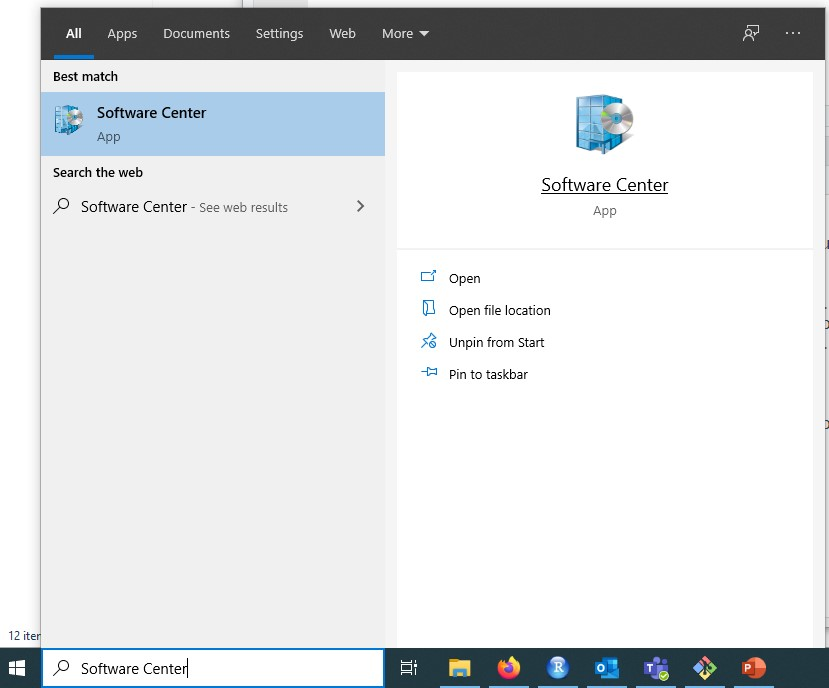
\includegraphics{files/00-start/software_center.jpg}

RStudio:n voi asentaa Software Centeristä, ja RStudion pitäisi sen jälkeen olla käytettävissä.

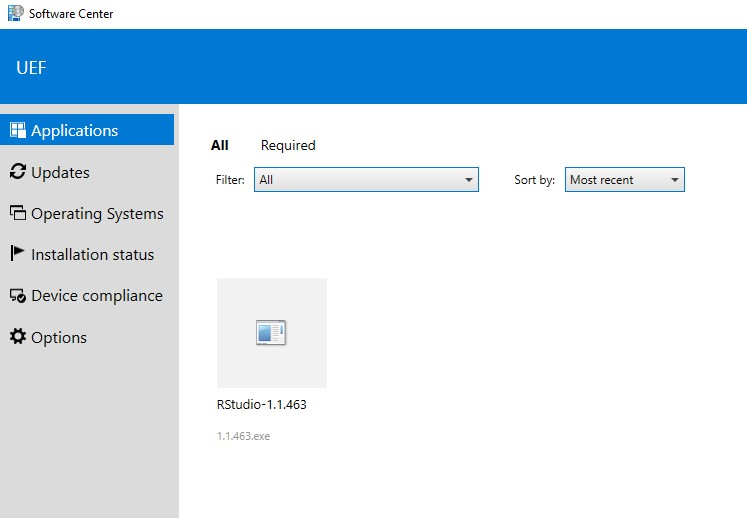
\includegraphics{files/00-start/RStudio_sc.jpg}

\hypertarget{rstudion-kuxe4yttuxf6}{%
\section*{RStudion käyttö}\label{rstudion-kuxe4yttuxf6}}
\addcontentsline{toc}{section}{RStudion käyttö}

RStudion näkymässä on neljä osaa:

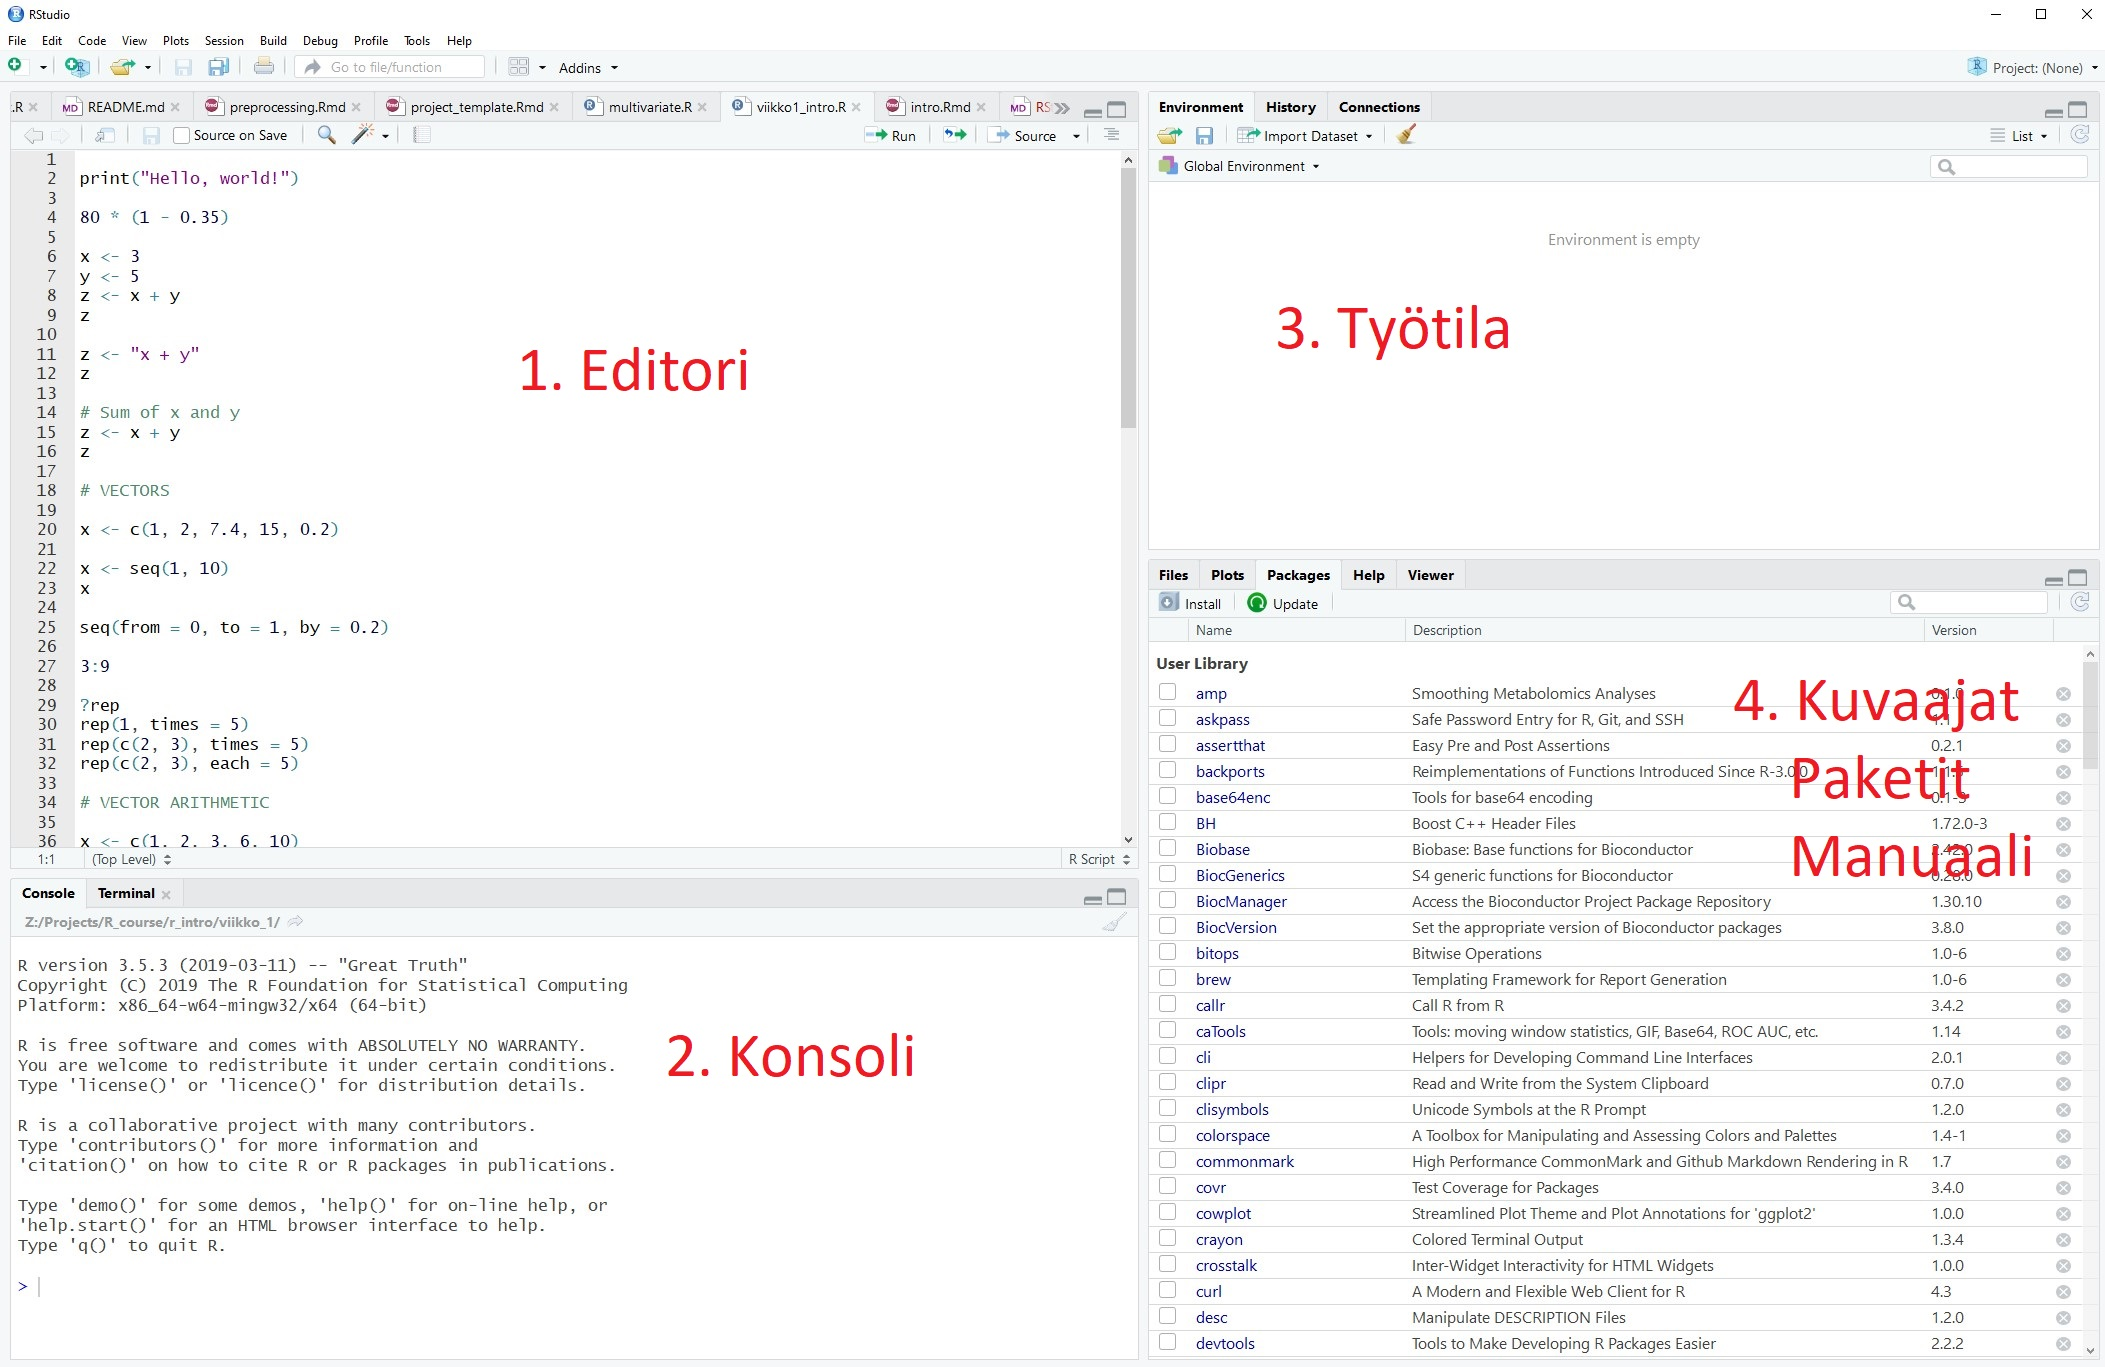
\includegraphics{files/00-start/RStudio_tutorial_edited.jpg}

\hypertarget{editori.}{%
\subsubsection*{1. Editori.}\label{editori.}}
\addcontentsline{toc}{subsubsection}{1. Editori.}

Editorilla kirjoitetaan R-koodia sisältäviä tiedostoja, eli R-skriptejä. Uuden skriptin saa auki painamalla File -\textgreater{} New File -\textgreater{} R Script (tai Ctrl + Shift + N). Skripteihin tutustutaan myöhemmin kurssilla, mutta ne ovat yksinkertaisuudessaan kokoelma R-komentoja, jotka yhdessä tekevät jotain, esimerkiksi analysoivat jonkin tutkimusprojektin datan tai piirtävät valmiista tuloksista kuvaajia.

Editoriin kirjoitettua koodia voi ajaa rivi kerrallaan painamalla rivin kohdalla Ctrl + Enter. Useamman rivin voi myös maalata ja suorittaa kerrallaan. Yläreunassa oleva ``Source''-nappi ajaa kaiken nykyisen tiedoston koodin.

R-skriptejä voi tallentaa ihan kuin muitakin tiedostoja. R-skpriptien tiedostopääte on .R

\hypertarget{konsoli.}{%
\subsubsection*{2. Konsoli.}\label{konsoli.}}
\addcontentsline{toc}{subsubsection}{2. Konsoli.}

Konsolissa ``ajetaan'' eli suoritetaan R-komentoja. Jos editoriin kirjoitettua koodia ajetaan, RStudio ajaa komennot automaattisesti konsolissa. Konsolissa pelkkä Enter riittää koodirivin suorittamiseen. Voit kokeilla kirjoittaa konsoliin jonkun laskutoimituksen, kuten \texttt{2\ *\ 3} ja painaa Enter, jolloin tuloksen pitäisi tulostua konsoliin. Voit myös kokeilla kirjoittaa laskuja editoriin, ja painaa Ctrl + Enter, jolloin pitäisi tapahtua sama asia.

Suurin ero konsolin ja editorin välillä on se, että \textbf{konsoliin kirjoitetut komennot eivät tallennu mihinkään tiedostoon}. Jos siis haluat säilyttää koodisi, se tulee kirjoittaa editoriin ja tallentaa .R-tiedostoon. Saman istunnon aikana tehtyjä komentoja voi konsolissa selata ylös- ja alas-nuolila.

Moodlen ohjeissa ja videoissa käytetään R:ää puhtaasta R-konsolista. Voit siis kuvitella, että kurssin videoissa näkyy vain RStudion tämä osa, ja muut osat ovat vain helpottamassa työtäsi.

\hypertarget{tyuxf6tila}{%
\subsubsection*{3. Työtila}\label{tyuxf6tila}}
\addcontentsline{toc}{subsubsection}{3. Työtila}

Työtilassa näkyvät R-istunnon aikana luodut muuttujat. Näistä lisää ensimmäisen viikon materiaalissa.

\hypertarget{kuvaajat-paketit-manuaali}{%
\subsubsection*{4. Kuvaajat / Paketit / Manuaali}\label{kuvaajat-paketit-manuaali}}
\addcontentsline{toc}{subsubsection}{4. Kuvaajat / Paketit / Manuaali}

Tässä osassa on monta käytännöllistä välilehteä:

\begin{itemize}
\tightlist
\item
  Plots: tänne ilmestyvät R:llä piirretyt kuvaajat
\item
  Packages: Täältä voi hallita asennettuja paketteja (alla ohjeet tällä kurssilla tarvittavien pakettien asennukseen)
\item
  Help: Täällä voi selata R:n manuaalia, jossa on ohjeet jokaiselle R-komennolla. Voit kokeilla ajaa editorissa tai konsolissa komennon \texttt{?print}, joka avaa \texttt{print}-funktion ohjesivun.
\end{itemize}

Kun tehtävät tallentaa tällä tavalla, voi ensi kerralla vain yksinkertaisesti ajaa skriptin haluamaansa tehtävään asti.

\hypertarget{rcourse-paketin-asentaminen}{%
\section*{Rcourse-paketin asentaminen}\label{rcourse-paketin-asentaminen}}
\addcontentsline{toc}{section}{Rcourse-paketin asentaminen}

\hypertarget{r-paketit}{%
\subsection*{R-paketit}\label{r-paketit}}
\addcontentsline{toc}{subsection}{R-paketit}

R-ohjelmoinnissa asennetaan usein R-paketteja. Paketit ovat kokonaisuuksia, jotka lisäävät R:ään ominaisuuksia. Esimerkiksi tälle kurssille tarvittava paketti sisältää harjoitustehtäviä kurssin aihepiireistä sekä loppukokeen, jonka perusteella kurssin suoritus arvioidaan.

\hypertarget{asentaminen}{%
\subsection*{Asentaminen}\label{asentaminen}}
\addcontentsline{toc}{subsection}{Asentaminen}

Rcourse-paketti asennetaan suorittamalla seuraava koodi R:ssä. Kopioi koodi joko R-skriptiin ja aja se tai kopioi se suoraan Console-ikkunaan ja paina Enter-näppäintä.

\begin{Shaded}
\begin{Highlighting}[]
\FunctionTok{source}\NormalTok{(}\FunctionTok{url}\NormalTok{(}\StringTok{"http://users.jyu.fi/\textasciitilde{}santikka/Rcourse/install.R"}\NormalTok{))}
\end{Highlighting}
\end{Shaded}

Tämän jälkeen paketti tulee ottaa käyttöön

\begin{Shaded}
\begin{Highlighting}[]
\FunctionTok{library}\NormalTok{(Rcourse)}
\end{Highlighting}
\end{Shaded}

Komento \texttt{info()} tulostaa paketin ohjeet (ensimmäisellä käyttökerralla kieli on englanti). Voit vaihtaa kielen suomeksi näin:

\begin{Shaded}
\begin{Highlighting}[]
\FunctionTok{select\_language}\NormalTok{(}\StringTok{"finnish"}\NormalTok{)}
\end{Highlighting}
\end{Shaded}

Jos haluat, että kielivalinta säilyy R-istunnosta toiseen, tulee asettaa seuraava argumentti:

\begin{Shaded}
\begin{Highlighting}[]
\FunctionTok{select\_language}\NormalTok{(}\StringTok{"finnish"}\NormalTok{, }\AttributeTok{save\_selection =} \ConstantTok{TRUE}\NormalTok{)}
\end{Highlighting}
\end{Shaded}

Huomaa, että kielen vaihtuessa myös joidenkin pakettiin liittyvien funktioiden nimet vaihtuvat.
Tarkastele vielä suomenkielisiä komentoja:

\begin{Shaded}
\begin{Highlighting}[]
\FunctionTok{ohje}\NormalTok{()}
\end{Highlighting}
\end{Shaded}

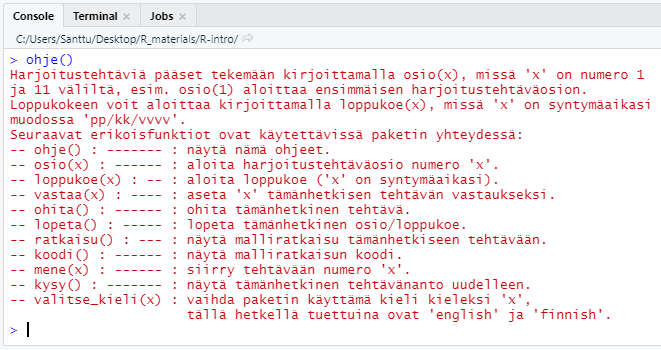
\includegraphics{files/00-start/Rcourse_package_info.png}

Aloita sitten osion 1 harjoitustehtävien suorittaminen komennolla

\begin{Shaded}
\begin{Highlighting}[]
\FunctionTok{osio}\NormalTok{(}\DecValTok{1}\NormalTok{)}
\end{Highlighting}
\end{Shaded}

Kun olet suorittanut harjoitusosion 1, voit jatkaa seuraavaan osioon. Osiot 1-8 ovat pakollisia (tentit kysyvät näiden osioiden sisältöjä) ja osiot 9-11 ovat lisämateriaalia kiinnostuneille (ei kysytä tentissä).

\hypertarget{opiskelu-ja-tenttiminen-rcourse-paketin-avulla}{%
\subsection*{Opiskelu ja tenttiminen Rcourse-paketin avulla}\label{opiskelu-ja-tenttiminen-rcourse-paketin-avulla}}
\addcontentsline{toc}{subsection}{Opiskelu ja tenttiminen Rcourse-paketin avulla}

Kurssin harjoitustehtävät suoritetaan käyttäen Rcourse-pakettia, eli 1. osion voi aloittaa komennolla

\begin{Shaded}
\begin{Highlighting}[]
\FunctionTok{osio}\NormalTok{(}\DecValTok{1}\NormalTok{)}
\end{Highlighting}
\end{Shaded}

Lisäksi tenttiminen onnistuu vastaavasti funktiolla \texttt{loppukoe(x)}, mutta tällöin merkin \texttt{x} tilalle on annettava oma syntymäaika muodossa ``dd/mm/yyyy''. Esim. henkilö joka on syntynyt 1. tammikuuta 1990 antaisi

\begin{Shaded}
\begin{Highlighting}[]
\FunctionTok{loppukoe}\NormalTok{(}\StringTok{"01/01/1990"}\NormalTok{)}
\end{Highlighting}
\end{Shaded}

\hypertarget{tehtuxe4vien-tallentaminen-skripteihin-rstudiolla}{%
\subsection*{Tehtävien tallentaminen skripteihin RStudiolla}\label{tehtuxe4vien-tallentaminen-skripteihin-rstudiolla}}
\addcontentsline{toc}{subsection}{Tehtävien tallentaminen skripteihin RStudiolla}

Suurin osa kurssin tehtävistä on melko lyhyitä, joten ne voi tarvittaessa tehdä suoraan konsoliin. Suosittelen kuitenkin kirjoittamaan varsinkin pidemmät ja monimutkaisemmat tehtävät muistiin editoriin. Suosittelenkin tekemään jokaista osiota varten erillisen R-skriptin, joka sisältää itse tehtävien tarvitseman koodin sekä palautuskomennot. Tällainen skripti näyttää jotakuinkin tältä:

\begin{Shaded}
\begin{Highlighting}[]
\CommentTok{\# Teht 1}
\NormalTok{vast }\OtherTok{\textless{}{-}} \DecValTok{1}
\FunctionTok{tarkista}\NormalTok{(vast)}

\CommentTok{\# Teht 2}
\NormalTok{vast }\OtherTok{\textless{}{-}} \FunctionTok{c}\NormalTok{(}\DecValTok{1}\NormalTok{, }\DecValTok{2}\NormalTok{, }\DecValTok{3}\NormalTok{)}
\FunctionTok{tarkista}\NormalTok{(vast)}

\CommentTok{\# Teht 3}
\NormalTok{vast }\OtherTok{\textless{}{-}} \StringTok{"jotain"}
\FunctionTok{tarkista}\NormalTok{(vast)}
\end{Highlighting}
\end{Shaded}

Mikäli käytät nimen \texttt{vast} sijasta jotain muuta nimeä, niin sinun on käytettävä samaa nimä myös tarkista-funktion argumenttina!

\hypertarget{intro}{%
\chapter{Johdanto}\label{intro}}

\hypertarget{what_R}{%
\section{Mikä R on ja mitä sillä tehdään?}\label{what_R}}

Ohjelmoinnin tavoitteena on kirjoittaa eli koodata ohjelma, joka suorittaa jonkun halutun tehtävän. Ohjelma koostuu useista komennoista, joista jokainen tekee jotain hyvin yksinkertaista.

R on tehty ensisijaisesti tilastotiedettä ja data-analyysiä varten. R:llä kirjoitetaan yleensä lyhyitä ohjelmia, joita kutsutaan skripteiksi. R:llä ei siis ole tarkoitus kehittää esimerkiksi pelejä, tai muita ohjelmia joissa on graafinen käyttöliittymä, kuten vaikkapa Photoshop. R ei myöskään ole web-ohjelmointiin tarkoitettu kieli (vaikka oikeilla paketeilla R:lläkin pystyy tekemään web-sovelluksia).

R on korkean tason ohjelmointikieli. Tämä tarkoittaa sitä, että R:ssä on paljon valmiita komentoja, joiden ``alta'' löytyy paljon lisää koodia, johon R-ohjelmoijan ei kuitenkaan tarvitse itse koskea. Esimerkiksi tilastollinen t-testi vaatii useita matemaattisia välivaiheita, mutta R-ohjelmoija voi suorittaa testin yhdellä komennolla (\texttt{t.test}) joka antaa kaikki tarvittavat tiedot testistä.

R:n käyttöä ja ohjelmointia oppii parhaiten tekemällä. Tässä dokumentaatiossa on tekstin väliin upotettu R-koodia harmaissa laatikoissa, kuten alla olevassa esimerkissä. Kahdella ruudulla eli \texttt{\#\#}-merkinnällä alkavat rivit eivät ole koodia vaan koodin ajamisen aiheuttamia tulosteita (output). Otetaan ensimmäiseksi esimerkiksi klassinen \href{https://en.wikipedia.org/wiki/\%22Hello,_World!\%22_program}{``Hello, world!''}-komento:

\begin{Shaded}
\begin{Highlighting}[]
\FunctionTok{print}\NormalTok{(}\StringTok{"Hello, world!"}\NormalTok{)}
\end{Highlighting}
\end{Shaded}

\begin{verbatim}
## [1] "Hello, world!"
\end{verbatim}

\texttt{print}-funktio tulostaa sille annetun tekstin konsoliin. \texttt{print} on kätevä funktio mm. ohjelman toiminnan testaamiseen ja pidemmän ohjelman etenemisen seurantaan. R:ää voi käyttää myös laskimen sijaan. Alla olevassa esimerkissä lasketaan kuinka paljon jää hintaa 80 euron hintaiselle tuotteelle 35\% alennuksen jälkeen.

\begin{Shaded}
\begin{Highlighting}[]
\DecValTok{80} \SpecialCharTok{*}\NormalTok{ (}\DecValTok{1} \SpecialCharTok{{-}} \FloatTok{0.35}\NormalTok{)}
\end{Highlighting}
\end{Shaded}

\begin{verbatim}
## [1] 52
\end{verbatim}

Yksittäisten komentojen ajamisesta ei kuitenkaan ole yleensä hyötyä, ellei tuloksia voi tallentaa johonkin. Ohjelmointikielissä tietoja tallennetaan muuttujiin, joita käsitellään seuraavaksi.

\hypertarget{variables_and_vectors}{%
\chapter{Muuttujat ja vektorit}\label{variables_and_vectors}}

\hypertarget{variables}{%
\section{Muuttujat}\label{variables}}

\textbf{Muuttujat} (variables) ovat yksi tärkeimmistä ohjelmointikielien rakenteista. Muuttujien tehtävä on säilyttää tietoa ja tuloksia edellisistä laskutoimituksista. Alla on yksinkertainen esimerkki muuttujien käytöstä R:ssä.

\begin{Shaded}
\begin{Highlighting}[]
\NormalTok{x }\OtherTok{\textless{}{-}} \DecValTok{3}
\NormalTok{y }\OtherTok{\textless{}{-}} \DecValTok{5}
\NormalTok{z }\OtherTok{\textless{}{-}}\NormalTok{ x }\SpecialCharTok{+}\NormalTok{ y}

\NormalTok{z}
\end{Highlighting}
\end{Shaded}

\begin{verbatim}
## [1] 8
\end{verbatim}

Edellisessä esimerkissä \textbf{sijoitetaan (assign)} eli tallennetaan muuttujaan x arvo 3 ja muuttujaan y arvo 4. Sen jälkeen muuttujien x ja y summa sijoitetaan muuttujaan z, jonka jälkeen tulostetaan muuttujan z arvo.
\texttt{\textless{}-} on R:n \textbf{sijoitusoperaattori} (myös yhtä kuin-merkki \texttt{=} toimii melkein aina, mutta \texttt{\textless{}-} merkin käyttöä suositellaan vahvasti).

Mutta miten muuttujan z arvo tulostui konsoliin, vaikka koodissa ei käytetty funktiota \texttt{print}? R:n erikoisominaisuus moneen muuhun ohjelmointikieleen verrattuna on se, että print-käskyä ei tarvitse aina kirjoittaa, vaan pelkästään muuttujan (tai laskutoimituksen) kirjoittaminen tulostaa arvon konsoliin, kuten alla oleva koodi havainnollistaa:

\begin{Shaded}
\begin{Highlighting}[]
\NormalTok{z}
\FunctionTok{print}\NormalTok{(z)}

\NormalTok{x }\SpecialCharTok{+}\NormalTok{ y}
\FunctionTok{print}\NormalTok{(x }\SpecialCharTok{+}\NormalTok{ y)}

\DecValTok{3} \SpecialCharTok{+} \DecValTok{5}
\FunctionTok{print}\NormalTok{(}\DecValTok{3} \SpecialCharTok{+} \DecValTok{5}\NormalTok{)}
\end{Highlighting}
\end{Shaded}

Muuttujiin voi sijoittaa muutakin kuin yksittäisiä lukuja, kuten merkkijonoja (strings), vektoreita, tai paljon monimutkaisempiakin rakenteita.

\begin{Shaded}
\begin{Highlighting}[]
\NormalTok{x }\OtherTok{\textless{}{-}} \StringTok{"Hello world"}
\NormalTok{x}
\end{Highlighting}
\end{Shaded}

\begin{verbatim}
## [1] "Hello world"
\end{verbatim}

\hypertarget{comments}{%
\section{Kommentit}\label{comments}}

Myöhemmin vastaan tulevassa koodissa käytetään kommentteja. Kommentit ovat koodin oheen kirjoitettua tekstiä, joka ei ole ohjelmointikieltä, ja joka ohitetaan koodia ajettaessa. Kommenttien tarkoitus on kuvailla koodin toimintaa. Oman koodin kommentointia on hyvä harjoitella alusta lähtien, vaikka ensimmäisten tehtävien koodi onkin hyvin yksinkertaista. R:ssä kommentit merkataan \texttt{\#}-symbolilla. Edellinen esimerkki kommentoituna voisi näyttää jotakuinkin tältä:

\begin{Shaded}
\begin{Highlighting}[]
\CommentTok{\# Assign arbitrary numbers to two variables}
\NormalTok{x }\OtherTok{\textless{}{-}} \DecValTok{3}
\NormalTok{y }\OtherTok{\textless{}{-}} \DecValTok{5}
\CommentTok{\# Sum of two variables}
\NormalTok{z }\OtherTok{\textless{}{-}}\NormalTok{ x }\SpecialCharTok{+}\NormalTok{ y}
\CommentTok{\# Print the results}
\NormalTok{z}
\end{Highlighting}
\end{Shaded}

\begin{verbatim}
## [1] 8
\end{verbatim}

\hypertarget{vectors}{%
\section{Vektorit}\label{vectors}}

Nyt kun muuttujat ovat tuttuja, voimme siirtyä käsittelemään vektoreita (vector). R:n vektorit ovat yksinkertaisia järjestettyjä tietorakenteita, jotka koostuvat alkioista (elements), esimerkiksi desimaaliluvuista. Alla oleva esimerkki sijoittaa muuttujaan x vektorin, joka sisältää 5 lukua.

\begin{Shaded}
\begin{Highlighting}[]
\NormalTok{x }\OtherTok{\textless{}{-}} \FunctionTok{c}\NormalTok{(}\DecValTok{1}\NormalTok{, }\DecValTok{2}\NormalTok{, }\FloatTok{7.4}\NormalTok{, }\DecValTok{15}\NormalTok{, }\FloatTok{0.2}\NormalTok{)}
\NormalTok{x}
\end{Highlighting}
\end{Shaded}

\begin{verbatim}
## [1]  1.0  2.0  7.4 15.0  0.2
\end{verbatim}

Yksinkertaisin tapa tehdä vektori R:ssä on käyttää \texttt{c}-funktiota, joka luo vektorin, jossa on sille annetut arvot annetussa järjestyksessä. Monet R-kielen komennot ja funktiot luovat vektoreita, alla muutama esimerkki:

\begin{Shaded}
\begin{Highlighting}[]
\CommentTok{\# Regular sequences}
\FunctionTok{seq}\NormalTok{(}\DecValTok{1}\NormalTok{, }\DecValTok{10}\NormalTok{)}
\end{Highlighting}
\end{Shaded}

\begin{verbatim}
##  [1]  1  2  3  4  5  6  7  8  9 10
\end{verbatim}

\begin{Shaded}
\begin{Highlighting}[]
\FunctionTok{seq}\NormalTok{(}\DecValTok{0}\NormalTok{, }\DecValTok{1}\NormalTok{, }\AttributeTok{by =} \FloatTok{0.2}\NormalTok{)}
\end{Highlighting}
\end{Shaded}

\begin{verbatim}
## [1] 0.0 0.2 0.4 0.6 0.8 1.0
\end{verbatim}

\begin{Shaded}
\begin{Highlighting}[]
\FunctionTok{seq\_len}\NormalTok{(}\DecValTok{6}\NormalTok{)}
\end{Highlighting}
\end{Shaded}

\begin{verbatim}
## [1] 1 2 3 4 5 6
\end{verbatim}

\begin{Shaded}
\begin{Highlighting}[]
\DecValTok{3}\SpecialCharTok{:}\DecValTok{9}
\end{Highlighting}
\end{Shaded}

\begin{verbatim}
## [1] 3 4 5 6 7 8 9
\end{verbatim}

\begin{Shaded}
\begin{Highlighting}[]
\CommentTok{\# Repeat values}
\FunctionTok{rep}\NormalTok{(}\DecValTok{1}\NormalTok{, }\DecValTok{5}\NormalTok{)}
\end{Highlighting}
\end{Shaded}

\begin{verbatim}
## [1] 1 1 1 1 1
\end{verbatim}

\begin{Shaded}
\begin{Highlighting}[]
\FunctionTok{rep}\NormalTok{(}\FunctionTok{c}\NormalTok{(}\DecValTok{1}\NormalTok{, }\DecValTok{2}\NormalTok{), }\DecValTok{3}\NormalTok{) }\CommentTok{\# Repeat vector c(1, 2) 3 times}
\end{Highlighting}
\end{Shaded}

\begin{verbatim}
## [1] 1 2 1 2 1 2
\end{verbatim}

\begin{Shaded}
\begin{Highlighting}[]
\FunctionTok{rep}\NormalTok{(}\FunctionTok{c}\NormalTok{(}\DecValTok{1}\NormalTok{, }\DecValTok{2}\NormalTok{, }\DecValTok{3}\NormalTok{), }\DecValTok{3}\NormalTok{) }\CommentTok{\# Repeat all values in vector c(1, 2, 3) 3 times}
\end{Highlighting}
\end{Shaded}

\begin{verbatim}
## [1] 1 2 3 1 2 3 1 2 3
\end{verbatim}

\hypertarget{vectorcalc}{%
\subsubsection{Vektorilaskentaa}\label{vectorcalc}}

Vektoreilla laskeminen on usein hyvin intuitiivista (lisää vaaranpaikoista myöhemmin). Kun vektoriin kohdistetaan laskutoimintoja, sama operaatio tehdään kaikille vektorin alkioille (engl. vectorization).

\begin{Shaded}
\begin{Highlighting}[]
\NormalTok{x }\OtherTok{\textless{}{-}} \FunctionTok{c}\NormalTok{(}\DecValTok{1}\NormalTok{, }\DecValTok{2}\NormalTok{, }\DecValTok{3}\NormalTok{, }\DecValTok{6}\NormalTok{, }\DecValTok{10}\NormalTok{)}
\NormalTok{x }\SpecialCharTok{*} \DecValTok{2}
\end{Highlighting}
\end{Shaded}

\begin{verbatim}
## [1]  2  4  6 12 20
\end{verbatim}

\begin{Shaded}
\begin{Highlighting}[]
\NormalTok{x }\SpecialCharTok{/} \DecValTok{2} \SpecialCharTok{+} \DecValTok{1}
\end{Highlighting}
\end{Shaded}

\begin{verbatim}
## [1] 1.5 2.0 2.5 4.0 6.0
\end{verbatim}

Entä jos vektoreita lisää toisiinsa, tai kertoo keskenään? Jos vektorit ovat samanpituisia, operaatio toteutetaan alkio kerrallaan. Jos vektorit ovat eripituisia, R yrittää kierrättää (recycle) lyhyempää vektoria niin, että siitä tulee yhtä pitkä kuin pidempi vektori. Tämän jälkeen operaatio suoritetaan alkio kerrallaan (itse asiassa näin tapahtui myös aiemmissa esimerkeissä, kun vektori kerrottiin yksittäisellä luvulla. R:ssä yksittäiset luvut ovat vektoreita, joiden pituus on 1). Jos kierrätys ei onnistu, eli pidemmän vektorin pituus ei ole jaollinen lyhyemmän pituudella, R antaa virheilmoituksen.

\begin{Shaded}
\begin{Highlighting}[]
\NormalTok{x }\OtherTok{\textless{}{-}} \FunctionTok{c}\NormalTok{(}\DecValTok{1}\NormalTok{, }\DecValTok{2}\NormalTok{, }\DecValTok{3}\NormalTok{, }\DecValTok{6}\NormalTok{, }\DecValTok{10}\NormalTok{, }\DecValTok{2}\NormalTok{)}
\NormalTok{y }\OtherTok{\textless{}{-}} \FunctionTok{c}\NormalTok{(}\DecValTok{1}\NormalTok{, }\DecValTok{1}\NormalTok{, }\DecValTok{1}\NormalTok{, }\DecValTok{3}\NormalTok{, }\DecValTok{3}\NormalTok{, }\DecValTok{3}\NormalTok{) }\CommentTok{\# or rep(c(1, 3), each = 3)}
\NormalTok{z }\OtherTok{\textless{}{-}} \FunctionTok{c}\NormalTok{(}\DecValTok{2}\NormalTok{, }\DecValTok{4}\NormalTok{)}

\NormalTok{x }\SpecialCharTok{+}\NormalTok{ y }\CommentTok{\# Element{-}wise sum}
\end{Highlighting}
\end{Shaded}

\begin{verbatim}
## [1]  2  3  4  9 13  5
\end{verbatim}

\begin{Shaded}
\begin{Highlighting}[]
\NormalTok{x }\SpecialCharTok{*}\NormalTok{ y }\CommentTok{\# Element{-}wise multipliocation}
\end{Highlighting}
\end{Shaded}

\begin{verbatim}
## [1]  1  2  3 18 30  6
\end{verbatim}

\begin{Shaded}
\begin{Highlighting}[]
\NormalTok{x }\SpecialCharTok{+}\NormalTok{ z}
\end{Highlighting}
\end{Shaded}

\begin{verbatim}
## [1]  3  6  5 10 12  6
\end{verbatim}

R:ssä on myös paljon funktioita, joilla voi laskea vektoreista erilaisia tunnuslukuja, kuten keskiarvon, mediaanin, keskihajonnan jne.

\begin{Shaded}
\begin{Highlighting}[]
\NormalTok{x }\OtherTok{\textless{}{-}} \FunctionTok{c}\NormalTok{(}\DecValTok{1}\NormalTok{, }\DecValTok{2}\NormalTok{, }\DecValTok{3}\NormalTok{, }\DecValTok{6}\NormalTok{, }\DecValTok{10}\NormalTok{, }\DecValTok{2}\NormalTok{)}
\CommentTok{\# Sample mean (average)}
\FunctionTok{mean}\NormalTok{(x)}
\end{Highlighting}
\end{Shaded}

\begin{verbatim}
## [1] 4
\end{verbatim}

\begin{Shaded}
\begin{Highlighting}[]
\CommentTok{\# Standard deviation}
\FunctionTok{sd}\NormalTok{(x)}
\end{Highlighting}
\end{Shaded}

\begin{verbatim}
## [1] 3.405877
\end{verbatim}

\begin{Shaded}
\begin{Highlighting}[]
\CommentTok{\# Sum}
\FunctionTok{sum}\NormalTok{(x)}
\end{Highlighting}
\end{Shaded}

\begin{verbatim}
## [1] 24
\end{verbatim}

\hypertarget{ei-numeeriset-vektorit}{%
\subsection{Ei-numeeriset vektorit}\label{ei-numeeriset-vektorit}}

\hypertarget{merkkijonovektorit}{%
\subsubsection{Merkkijonovektorit}\label{merkkijonovektorit}}

Vektorien ei ole pakko sisältää lukuja. Vektorit voivat sisältää esimerkiksi merkkijonoja, kuten alussa nähty ``Hello, world!''. Merkkijonotyypin nimi R:ssä on \texttt{character}.

\begin{Shaded}
\begin{Highlighting}[]
\NormalTok{x }\OtherTok{\textless{}{-}} \FunctionTok{c}\NormalTok{(}\StringTok{"Hello, world!"}\NormalTok{, }\StringTok{"R is the best"}\NormalTok{, }\StringTok{"I"}\NormalTok{, }\StringTok{"like"}\NormalTok{, }\StringTok{"programming"}\NormalTok{, }\StringTok{"!"}\NormalTok{)}
\NormalTok{x}
\end{Highlighting}
\end{Shaded}

\begin{verbatim}
## [1] "Hello, world!" "R is the best" "I"             "like"         
## [5] "programming"   "!"
\end{verbatim}

Merkkijonovektoreiden muokkausta varten on omia funktiota, tärkeimpinä \texttt{paste} ja \texttt{paste0}, jotka yhdistävät merkkijonoja toisiinsa. Myös numeerisia vektoreita voi antaa näille funktioille, ja ne muutetaan merkkijonoiksi.

\begin{Shaded}
\begin{Highlighting}[]
\NormalTok{first\_names }\OtherTok{\textless{}{-}} \FunctionTok{c}\NormalTok{(}\StringTok{"Diana"}\NormalTok{, }\StringTok{"Peter"}\NormalTok{, }\StringTok{"Bruce"}\NormalTok{)}
\NormalTok{last\_names }\OtherTok{\textless{}{-}} \FunctionTok{c}\NormalTok{(}\StringTok{"Prince"}\NormalTok{, }\StringTok{"Parker"}\NormalTok{, }\StringTok{"Wayne"}\NormalTok{)}
\FunctionTok{paste}\NormalTok{(first\_names, last\_names)}
\end{Highlighting}
\end{Shaded}

\begin{verbatim}
## [1] "Diana Prince" "Peter Parker" "Bruce Wayne"
\end{verbatim}

\begin{Shaded}
\begin{Highlighting}[]
\NormalTok{students }\OtherTok{\textless{}{-}} \FunctionTok{paste0}\NormalTok{(}\StringTok{"Student\_"}\NormalTok{, }\DecValTok{1}\SpecialCharTok{:}\DecValTok{5}\NormalTok{)}
\end{Highlighting}
\end{Shaded}

\hypertarget{loogiset-vektorit}{%
\subsubsection{Loogiset vektorit}\label{loogiset-vektorit}}

Kolmas yleinen vektorityyppi on looginen vektori, joka sisältää arvoja \texttt{TRUE} eli tosi tai \texttt{FALSE} eli epätosi. Loogisia vektoreita käytetään yleensä joko merkitsemään binäärisiä muuttuja (esimerkiksi paastosiko koehenkilö ennen näytteenottoa) tai vektorien ja matriisien indeksoinnissa (tästä lisää pian). Tällöin loogisia vektoreita syntyy erilaisten loogisten operaattorien avulla:

\begin{Shaded}
\begin{Highlighting}[]
\NormalTok{x }\OtherTok{\textless{}{-}} \FunctionTok{c}\NormalTok{(}\DecValTok{1}\NormalTok{, }\DecValTok{2}\NormalTok{, }\DecValTok{3}\NormalTok{, }\DecValTok{6}\NormalTok{, }\DecValTok{10}\NormalTok{, }\DecValTok{2}\NormalTok{)}

\NormalTok{x }\SpecialCharTok{\textgreater{}} \DecValTok{3} \CommentTok{\# Is the element of x greater than 3?}
\end{Highlighting}
\end{Shaded}

\begin{verbatim}
## [1] FALSE FALSE FALSE  TRUE  TRUE FALSE
\end{verbatim}

\begin{Shaded}
\begin{Highlighting}[]
\NormalTok{x }\SpecialCharTok{\textgreater{}=} \DecValTok{3} \CommentTok{\# Greater or equal to three=}
\end{Highlighting}
\end{Shaded}

\begin{verbatim}
## [1] FALSE FALSE  TRUE  TRUE  TRUE FALSE
\end{verbatim}

\begin{Shaded}
\begin{Highlighting}[]
\NormalTok{x }\SpecialCharTok{==} \DecValTok{6} \CommentTok{\# Equal to 6?}
\end{Highlighting}
\end{Shaded}

\begin{verbatim}
## [1] FALSE FALSE FALSE  TRUE FALSE FALSE
\end{verbatim}

\begin{Shaded}
\begin{Highlighting}[]
\NormalTok{x }\SpecialCharTok{!=} \DecValTok{2} \CommentTok{\# Not equal to 2?}
\end{Highlighting}
\end{Shaded}

\begin{verbatim}
## [1]  TRUE FALSE  TRUE  TRUE  TRUE FALSE
\end{verbatim}

\hypertarget{loogiset-vektorit-ja-matematiikka}{%
\subsubsection{Loogiset vektorit ja matematiikka}\label{loogiset-vektorit-ja-matematiikka}}

Jos loogiselle vektorille tekee operaation, joka odottaa numeerista vektoria, R muuttaa automaattisesti arvot \texttt{TRUE} ykkösiksi ja arvot \texttt{FALSE} nolliksi. Tämä on erityisen hyödyllistä käytettäessä funktiota \texttt{sum}. Tällä tavalla saadaan helposti tietää esim. kuinka moni vektorin alkio täyttää tietyn ehdon:

\begin{Shaded}
\begin{Highlighting}[]
\NormalTok{x }\OtherTok{\textless{}{-}} \FunctionTok{c}\NormalTok{(}\DecValTok{1}\NormalTok{, }\DecValTok{3}\NormalTok{, }\DecValTok{5}\NormalTok{, }\DecValTok{2}\NormalTok{, }\DecValTok{19}\NormalTok{)}
\NormalTok{above\_3 }\OtherTok{\textless{}{-}}\NormalTok{ x }\SpecialCharTok{\textgreater{}} \DecValTok{3}

\CommentTok{\# Logical vector automatically converted to numeric}
\NormalTok{x }\SpecialCharTok{+} \DecValTok{1}
\end{Highlighting}
\end{Shaded}

\begin{verbatim}
## [1]  2  4  6  3 20
\end{verbatim}

\begin{Shaded}
\begin{Highlighting}[]
\CommentTok{\# how many elements of x are smaller than 10?}
\FunctionTok{sum}\NormalTok{(x }\SpecialCharTok{\textless{}} \DecValTok{10}\NormalTok{)}
\end{Highlighting}
\end{Shaded}

\begin{verbatim}
## [1] 4
\end{verbatim}

\hypertarget{vektorien-indeksointi-ja-osajoukon-valinta}{%
\subsection{Vektorien indeksointi ja osajoukon valinta}\label{vektorien-indeksointi-ja-osajoukon-valinta}}

Usein vektorista halutaan poimia vain tietyt arvot, esimerkiksi vain ensimmäiset 5 arvoa, tai vain arvot, jotka täyttävät tietyt ehdot. R:ssä vektorin indeksointiin käytetään hakasulkeita \texttt{{[}{]}}. Yleisin indeksointitapa on antaa hakasulkeiden sisään vektori kokonaislukuja, jotka vastaavat niiden alkioiden järjestyslukuja, jotka vektorista halutaan poimia (HUOM R:ssä indeksointi alkaa ykkösestä, ei nollasta!). Toinen vaihtoehto on käyttää loogista vektoria, jolloin vektorista poimitaan ne alkiot, joiden kohdalla loogisen vektorin arvo on TRUE. Tämä on yksinkertaisempaa kuin miltä se kuulostaa:

\begin{Shaded}
\begin{Highlighting}[]
\NormalTok{x }\OtherTok{\textless{}{-}} \FunctionTok{c}\NormalTok{(}\DecValTok{1}\NormalTok{, }\DecValTok{2}\NormalTok{, }\DecValTok{3}\NormalTok{, }\DecValTok{6}\NormalTok{, }\DecValTok{10}\NormalTok{, }\DecValTok{2}\NormalTok{)}

\CommentTok{\# Picking exact elements}
\NormalTok{x[}\DecValTok{2}\SpecialCharTok{:}\DecValTok{3}\NormalTok{] }\CommentTok{\# Second and third values}
\end{Highlighting}
\end{Shaded}

\begin{verbatim}
## [1] 2 3
\end{verbatim}

\begin{Shaded}
\begin{Highlighting}[]
\NormalTok{x[}\FunctionTok{c}\NormalTok{(}\DecValTok{4}\NormalTok{, }\DecValTok{5}\NormalTok{, }\DecValTok{1}\NormalTok{)] }\CommentTok{\# Note that the order does not have to be increasing}
\end{Highlighting}
\end{Shaded}

\begin{verbatim}
## [1]  6 10  1
\end{verbatim}

\begin{Shaded}
\begin{Highlighting}[]
\CommentTok{\# Using logical vector as condition}
\NormalTok{x[x }\SpecialCharTok{\textgreater{}} \DecValTok{3}\NormalTok{]}
\end{Highlighting}
\end{Shaded}

\begin{verbatim}
## [1]  6 10
\end{verbatim}

\begin{Shaded}
\begin{Highlighting}[]
\CommentTok{\# The condition can be based on another vector}
\NormalTok{characters }\OtherTok{\textless{}{-}} \FunctionTok{c}\NormalTok{(}\StringTok{"Yoda"}\NormalTok{, }\StringTok{"C{-}3PO"}\NormalTok{, }\StringTok{"Rey"}\NormalTok{, }\StringTok{"R2{-}D2"}\NormalTok{, }\StringTok{"Anakin"}\NormalTok{, }\StringTok{"Baby Yoda"}\NormalTok{)}
\NormalTok{heights }\OtherTok{\textless{}{-}} \FunctionTok{c}\NormalTok{(}\DecValTok{66}\NormalTok{, }\DecValTok{175}\NormalTok{, }\DecValTok{170}\NormalTok{, }\DecValTok{109}\NormalTok{, }\DecValTok{183}\NormalTok{, }\FloatTok{40.5}\NormalTok{)}
\CommentTok{\# Only characters shorter than 120 cm}
\NormalTok{characters[heights }\SpecialCharTok{\textless{}} \DecValTok{120}\NormalTok{]}
\end{Highlighting}
\end{Shaded}

\begin{verbatim}
## [1] "Yoda"      "R2-D2"     "Baby Yoda"
\end{verbatim}

\hypertarget{puuttuvat-arvot}{%
\subsection{Puuttuvat arvot}\label{puuttuvat-arvot}}

Monessa tutkimusprojektissa törmätään syystä tai toisesta jossain vaiheessa puuttuviin arvoihin. Hyvä esimerkki ovat seurantatutkimukset, jossa usein seurannan lopussa on jäljellä vähemmän koehenkilöitä kuin alussa.

Puuttuvia arvoja merkitään R:ssä symbolilla \texttt{NA} (not available). Puuttuvat arvot noudattavat yksinkertaista logiikkaa: mikä tahansa operaatio \texttt{NA}:lle antaa tulokseksi \texttt{NA}. Funktiot, jotka operoivat vektoreilla, kuten \texttt{sum} tai \texttt{mean} voidaan erikseen asettaa poistamaan puuttuvat arvot ennen summan, keskiarvon tms. laskemista.

\begin{Shaded}
\begin{Highlighting}[]
\NormalTok{missing }\OtherTok{\textless{}{-}} \FunctionTok{c}\NormalTok{(}\DecValTok{1}\NormalTok{, }\DecValTok{2}\NormalTok{, }\ConstantTok{NA}\NormalTok{, }\DecValTok{4}\NormalTok{, }\ConstantTok{NA}\NormalTok{, }\DecValTok{6}\NormalTok{)}
\NormalTok{full }\OtherTok{\textless{}{-}} \FunctionTok{seq}\NormalTok{(}\DecValTok{1}\NormalTok{, }\DecValTok{6}\NormalTok{)}

\CommentTok{\# Addition with NA returns NA}
\NormalTok{missing }\SpecialCharTok{+}\NormalTok{ full}
\end{Highlighting}
\end{Shaded}

\begin{verbatim}
## [1]  2  4 NA  8 NA 12
\end{verbatim}

\begin{Shaded}
\begin{Highlighting}[]
\CommentTok{\# Sum of vector with NAs returns NA}
\FunctionTok{sum}\NormalTok{(missing)}
\end{Highlighting}
\end{Shaded}

\begin{verbatim}
## [1] NA
\end{verbatim}

\begin{Shaded}
\begin{Highlighting}[]
\CommentTok{\# Removing NAs before summation}
\FunctionTok{sum}\NormalTok{(missing, }\AttributeTok{na.rm =} \ConstantTok{TRUE}\NormalTok{)}
\end{Highlighting}
\end{Shaded}

\begin{verbatim}
## [1] 13
\end{verbatim}

HUOM! Funktio \texttt{is.na} tarkistaa, onko jokin arvo puuttuva. Perinteinen yhtäsuuruuden testaaminen ei siis toimi.

\begin{Shaded}
\begin{Highlighting}[]
\CommentTok{\# Just returns NA}
\ConstantTok{NA} \SpecialCharTok{==} \ConstantTok{NA}
\end{Highlighting}
\end{Shaded}

\begin{verbatim}
## [1] NA
\end{verbatim}

\begin{Shaded}
\begin{Highlighting}[]
\CommentTok{\# Returns a logical value as expected}
\FunctionTok{is.na}\NormalTok{(}\ConstantTok{NA}\NormalTok{)}
\end{Highlighting}
\end{Shaded}

\begin{verbatim}
## [1] TRUE
\end{verbatim}

\begin{Shaded}
\begin{Highlighting}[]
\FunctionTok{is.na}\NormalTok{(}\DecValTok{1}\NormalTok{)}
\end{Highlighting}
\end{Shaded}

\begin{verbatim}
## [1] FALSE
\end{verbatim}

\begin{Shaded}
\begin{Highlighting}[]
\CommentTok{\# is.na operates element{-}wise on a vector}
\NormalTok{missing }\OtherTok{\textless{}{-}} \FunctionTok{c}\NormalTok{(}\DecValTok{1}\NormalTok{, }\DecValTok{2}\NormalTok{, }\ConstantTok{NA}\NormalTok{, }\DecValTok{4}\NormalTok{, }\ConstantTok{NA}\NormalTok{, }\DecValTok{6}\NormalTok{)}
\FunctionTok{is.na}\NormalTok{(missing)}
\end{Highlighting}
\end{Shaded}

\begin{verbatim}
## [1] FALSE FALSE  TRUE FALSE  TRUE FALSE
\end{verbatim}

\begin{Shaded}
\begin{Highlighting}[]
\CommentTok{\# complete.cases gives the data elements which do not have missing data. }
\CommentTok{\# It can be used with data frames also.}
\FunctionTok{complete.cases}\NormalTok{(missing)}
\end{Highlighting}
\end{Shaded}

\begin{verbatim}
## [1]  TRUE  TRUE FALSE  TRUE FALSE  TRUE
\end{verbatim}

\hypertarget{extra}{%
\section{Extra: Alkeistietotyypit ja erikoisarvot}\label{extra}}

Tässä lisätieto-osiossa käsitellään asioita, joita et välttämättä tarvitse kurssista suoriutuaksesi. Mikäli käytät R:ää enemmän, niin vastaan tulee enemmin tai myöhemmin ongelmia, joissa tarvitsee näitä taitoja. Voit palata näihin myöhemmin koska tahansa, kun haluat syventää ymmärrystäsi R:stä.

R on rakennettu sisäisesti siten, että vektorin kukin elementti on jotain alkeistietotyyppiä. R:ssä on valmiina neljä alkeistietotyyppiä:

\begin{itemize}
\tightlist
\item
  numeerinen (eli reaaliluku)
\item
  kokonaisluku (integer)
\item
  merkkijono (character)
\item
  kompleksiluku (complex)
\end{itemize}

Näistä tarpeellisimpia ovat numeerinen ja merkkijono. Kompleksilukua tarvitsee vain joissain erityistapauksissa ja kokonaisluvut ovat nykyään lähes aina tallennettu numeerisina.

\begin{Shaded}
\begin{Highlighting}[]
\CommentTok{\# Integers are usually stored as reals}
\NormalTok{x }\OtherTok{\textless{}{-}} \FunctionTok{c}\NormalTok{(}\DecValTok{1}\NormalTok{, }\DecValTok{2}\NormalTok{, }\DecValTok{3}\NormalTok{)}
\FunctionTok{class}\NormalTok{(x)}
\end{Highlighting}
\end{Shaded}

\begin{verbatim}
## [1] "numeric"
\end{verbatim}

\begin{Shaded}
\begin{Highlighting}[]
\CommentTok{\# You can create integers by adding capital L behind the number}
\NormalTok{x\_int }\OtherTok{\textless{}{-}} \FunctionTok{c}\NormalTok{(1L, 2L, 3L)}
\FunctionTok{class}\NormalTok{(x\_int)}
\end{Highlighting}
\end{Shaded}

\begin{verbatim}
## [1] "integer"
\end{verbatim}

\begin{Shaded}
\begin{Highlighting}[]
\CommentTok{\# Character strings (or just strings)}
\NormalTok{x\_char }\OtherTok{\textless{}{-}} \FunctionTok{c}\NormalTok{(}\StringTok{"I"}\NormalTok{, }\StringTok{"have"}\NormalTok{, }\StringTok{"a"}\NormalTok{, }\StringTok{"cat."}\NormalTok{)}
\FunctionTok{class}\NormalTok{(x\_char)}
\end{Highlighting}
\end{Shaded}

\begin{verbatim}
## [1] "character"
\end{verbatim}

\begin{Shaded}
\begin{Highlighting}[]
\CommentTok{\# Complex numbers}
\NormalTok{x\_comp }\OtherTok{\textless{}{-}} \FunctionTok{c}\NormalTok{(0i, }\DecValTok{2} \SpecialCharTok{+}\NormalTok{ 1i, }\DecValTok{1} \SpecialCharTok{{-}}\NormalTok{ 3i)}
\FunctionTok{class}\NormalTok{(x\_comp)}
\end{Highlighting}
\end{Shaded}

\begin{verbatim}
## [1] "complex"
\end{verbatim}

Joskus vektorin tiedot ovat väärässä muodossa, esim. merkkijonoina, mutta niitä haluttaisiin käsitellä numeroarvoina. Näihin operaatioihin on omat funktionsa. Tällöin voi kuitenkin tulla ongelmia, jos muutettava vektori ei ole helposti muutettavissa haluttuun muotoon.

\begin{Shaded}
\begin{Highlighting}[]
\CommentTok{\# Chacter string to numeric}
\FunctionTok{class}\NormalTok{(}\FunctionTok{as.numeric}\NormalTok{(x\_char))}
\end{Highlighting}
\end{Shaded}

\begin{verbatim}
## Warning: NAs introduced by coercion
\end{verbatim}

\begin{verbatim}
## [1] "numeric"
\end{verbatim}

\begin{Shaded}
\begin{Highlighting}[]
\CommentTok{\# If character contains only values it is easy}
\NormalTok{x\_char2 }\OtherTok{\textless{}{-}} \FunctionTok{c}\NormalTok{(}\StringTok{"0"}\NormalTok{, }\StringTok{"5"}\NormalTok{, }\StringTok{"6.5"}\NormalTok{)}
\FunctionTok{as.numeric}\NormalTok{(x\_char2)}
\end{Highlighting}
\end{Shaded}

\begin{verbatim}
## [1] 0.0 5.0 6.5
\end{verbatim}

\begin{Shaded}
\begin{Highlighting}[]
\CommentTok{\# Integer to numeric}
\NormalTok{x\_int\_to\_num }\OtherTok{\textless{}{-}} \FunctionTok{as.numeric}\NormalTok{(x\_int)}
\NormalTok{x\_int\_to\_num}
\end{Highlighting}
\end{Shaded}

\begin{verbatim}
## [1] 1 2 3
\end{verbatim}

\begin{Shaded}
\begin{Highlighting}[]
\FunctionTok{class}\NormalTok{(x\_int\_to\_num)}
\end{Highlighting}
\end{Shaded}

\begin{verbatim}
## [1] "numeric"
\end{verbatim}

\begin{Shaded}
\begin{Highlighting}[]
\CommentTok{\# Numeric to integer}
\NormalTok{x\_num\_to\_int }\OtherTok{\textless{}{-}} \FunctionTok{as.integer}\NormalTok{(x)}
\NormalTok{x\_num\_to\_int}
\end{Highlighting}
\end{Shaded}

\begin{verbatim}
## [1] 1 2 3
\end{verbatim}

\begin{Shaded}
\begin{Highlighting}[]
\FunctionTok{class}\NormalTok{(x\_num\_to\_int)}
\end{Highlighting}
\end{Shaded}

\begin{verbatim}
## [1] "integer"
\end{verbatim}

Vielä pari lisähuomiota puuttuvista arvoista (näitä ei tarvise usein) koskien niiden tietotyyppejä. Puuttuvalla arvolla on myös alkeistietotyyppi. Mikäli NA-arvon tietotyyppi tulee määritellä, niin sen voi tehdä seuraavasti. Jos luodaan muuttuja tai vektori, jossa on vain yksi arvo, joka on NA, niin se oletusarvoisesti looginen.

\begin{Shaded}
\begin{Highlighting}[]
\CommentTok{\# Specify a numeric NA value}
\ConstantTok{NA\_real\_}
\end{Highlighting}
\end{Shaded}

\begin{verbatim}
## [1] NA
\end{verbatim}

\begin{Shaded}
\begin{Highlighting}[]
\CommentTok{\# Specify a complex number NA value}
\ConstantTok{NA\_complex\_}
\end{Highlighting}
\end{Shaded}

\begin{verbatim}
## [1] NA
\end{verbatim}

\begin{Shaded}
\begin{Highlighting}[]
\CommentTok{\# Specify a integer number NA value}
\ConstantTok{NA\_integer\_}
\end{Highlighting}
\end{Shaded}

\begin{verbatim}
## [1] NA
\end{verbatim}

\begin{Shaded}
\begin{Highlighting}[]
\CommentTok{\# Specify a character NA value}
\ConstantTok{NA\_character\_}
\end{Highlighting}
\end{Shaded}

\begin{verbatim}
## [1] NA
\end{verbatim}

\begin{Shaded}
\begin{Highlighting}[]
\CommentTok{\# NA gives a logical type when evaluated alone}
\FunctionTok{class}\NormalTok{(}\ConstantTok{NA}\NormalTok{)}
\end{Highlighting}
\end{Shaded}

\begin{verbatim}
## [1] "logical"
\end{verbatim}

\begin{Shaded}
\begin{Highlighting}[]
\CommentTok{\# NA\_real\_ is numeric}
\FunctionTok{class}\NormalTok{(}\ConstantTok{NA\_real\_}\NormalTok{)}
\end{Highlighting}
\end{Shaded}

\begin{verbatim}
## [1] "numeric"
\end{verbatim}

\hypertarget{uxe4uxe4retuxf6n-ja-miinus-uxe4uxe4retuxf6n}{%
\subsection{Ääretön ja miinus ääretön}\label{uxe4uxe4retuxf6n-ja-miinus-uxe4uxe4retuxf6n}}

R:ssä on myös ääretön ja miinus ääretön. Ne on toteutettu samaan tapaan kuin puuttuva arvo, mutta niiden tarkasteluun on omat funktionsa. Ääretön ja miinus ääretön arvot syntyvät esimerkiksi silloin, kun nollasta poikkeavia lukuja jaetaan nollalla.

\begin{Shaded}
\begin{Highlighting}[]
\CommentTok{\# You can type in infinity or minus infinity if needed}
\NormalTok{x }\OtherTok{\textless{}{-}} \FunctionTok{c}\NormalTok{(}\DecValTok{1}\NormalTok{, }\DecValTok{2}\NormalTok{, }\ConstantTok{Inf}\NormalTok{, }\DecValTok{5}\NormalTok{, }\SpecialCharTok{{-}}\ConstantTok{Inf}\NormalTok{)}
\CommentTok{\# Use is.finite to determine if numbers are finite or not}
\FunctionTok{is.finite}\NormalTok{(x)}
\end{Highlighting}
\end{Shaded}

\begin{verbatim}
## [1]  TRUE  TRUE FALSE  TRUE FALSE
\end{verbatim}

\begin{Shaded}
\begin{Highlighting}[]
\CommentTok{\# Division by zero makes Inf or {-}Inf (unless 0/0)}
\NormalTok{x\_div\_zero }\OtherTok{\textless{}{-}} \FunctionTok{c}\NormalTok{(}\DecValTok{1}\NormalTok{, }\DecValTok{2}\NormalTok{, }\SpecialCharTok{{-}}\DecValTok{3}\NormalTok{) }\SpecialCharTok{/} \FunctionTok{c}\NormalTok{(}\DecValTok{3}\NormalTok{, }\DecValTok{0}\NormalTok{, }\DecValTok{0}\NormalTok{)}
\NormalTok{x\_div\_zero}
\end{Highlighting}
\end{Shaded}

\begin{verbatim}
## [1] 0.3333333       Inf      -Inf
\end{verbatim}

\begin{Shaded}
\begin{Highlighting}[]
\FunctionTok{is.finite}\NormalTok{(x\_div\_zero)}
\end{Highlighting}
\end{Shaded}

\begin{verbatim}
## [1]  TRUE FALSE FALSE
\end{verbatim}

\hypertarget{ei-numero}{%
\subsection{Ei-numero}\label{ei-numero}}

Mikäli R:ssä sattuu tekemään jonkin matemaattisen toimenpiteen, joka ei ole sallittu, esimerkiksi nollan jaon nollalla tai luvun -1 logaritmin, niin tämä tuottaa R:ssä tietotyypin, joka on \texttt{NaN} (lyhenne sanoista Not a Number). Mikäli \texttt{NaN}-arvoa tutkii funktiolla \texttt{is.finite} tai \texttt{is.na}, niin huomaa että \texttt{NaN} ei ole äärellinen ja \texttt{NaN} tulkitaan \texttt{NA}:ksi.

\begin{Shaded}
\begin{Highlighting}[]
\NormalTok{x\_div\_zero\_by\_zero }\OtherTok{\textless{}{-}} \DecValTok{0}\SpecialCharTok{/}\DecValTok{0}

\CommentTok{\# Tests for NaN}
\FunctionTok{is.nan}\NormalTok{(x\_div\_zero\_by\_zero)}
\end{Highlighting}
\end{Shaded}

\begin{verbatim}
## [1] TRUE
\end{verbatim}

\begin{Shaded}
\begin{Highlighting}[]
\CommentTok{\# Tests if it is finite}
\FunctionTok{is.finite}\NormalTok{(x\_div\_zero\_by\_zero)}
\end{Highlighting}
\end{Shaded}

\begin{verbatim}
## [1] FALSE
\end{verbatim}

\begin{Shaded}
\begin{Highlighting}[]
\CommentTok{\# Tests if it is NA (missing)}
\FunctionTok{is.na}\NormalTok{(x\_div\_zero\_by\_zero)}
\end{Highlighting}
\end{Shaded}

\begin{verbatim}
## [1] TRUE
\end{verbatim}

\hypertarget{data_types}{%
\chapter{Tietotyypit}\label{data_types}}

Tässä osassa tutustutaan neljään uuteen tietorakenteeseen:

\begin{itemize}
\tightlist
\item
  \protect\hyperlink{data-frame}{datakehikko (data.frame)}
\item
  \protect\hyperlink{matrix}{matriisi (matrix)}
\item
  \protect\hyperlink{array}{taulukko (array)}
\item
  \protect\hyperlink{list}{lista (list)}
\end{itemize}

Datakehikko on R:n objekti, jossa voidaan säilyttää aineistoa. Muuttujat ovat kehikon sarakkeita ja muuttujilla tulee aina olla nimi.

Matriisi voi olla joillekin tuttu käsite myös tilastotieteen tai matematiikan kursseilta, ja R:n matriisi vastaakin matemaattista matriisia. Tästä syystä matriisi on hyvin yleinen tietorakenne, johon ei voi olla törmäämättä jos käyttää R:ää tutkimuksessa. Matriisilla tehdään yleensä kuitenkin matemaattisia operaatioita, eikä se ensisijaisesti ole aineiston säilytyspaikka.

Taulukko on juuri sitä miltä se kuulostaa: vektorintapainen tietorakenne, johon tallennetaan alkioita (elements), joilla on kaikilla sama luokka (class), eli esimerkiksi lukuja. Ero vektoriin on se, että taulukolla on useampi ulottuvuus. Matriisi on erikoistapaus taulukosta, sillä matriisi on kaksiulotteinen taulukko. Matriisi vastaa siis oikeastaan paremmin sitä mielikuvaa, joka monelle tulee mieleen suomen kielen sanasta taulukko, ja matriisit ovatkin paljon yleisempiä kuin moniulotteiset taulukot.

Lista on järjestetty kokoelma alkioita, jotka voivat olla eri tyyppisiä objekteja.

Koska datakehikko on kaikista tärkein ja eniten käytetty tietotyyppi, niin aloitetaan siitä.

\hypertarget{data-frame}{%
\section{Datakehikko (data.frame)}\label{data-frame}}

Datakehikko on erittäin yleinen tietorakenne tiedon tallentamiseen R:ssä. Datakehikko on kaksiulotteinen tietorakenne, eli sillä on rivejä ja sarakkeita. Datakehikon sarakkeet muodostuvat vektoreista. Sarakevektorit voivat olla eri luokan vektoreita, mutta datakehikko asettaa lisärajoitteen: vektoreiden on oltava yhtä pitkiä. Yhden rivin sarakkeilla olevien arvojen ajatellaan koskevan yhtä havaintoa.

Luodaan datakehikko, jossa on kaksi muuttujaa, height ja weight, ja sijoitetaan niihin kahdeksan mittauksen tiedot. Huomionarvoista on se, että komennon \texttt{data.frame} sulkujen sisällä on käytettävä yhtäsuuruusmerkkiä (=) eikä sijoitusoperaattoria (\textless-). Tämä johtuu siitä, että teknisesti ottaen komento \texttt{data.frame} on funktio (funktioista lisää myöhemmin).

\begin{Shaded}
\begin{Highlighting}[]
\NormalTok{study\_data }\OtherTok{\textless{}{-}} \FunctionTok{data.frame}\NormalTok{(}\AttributeTok{ID =} \DecValTok{1}\SpecialCharTok{:}\DecValTok{8}\NormalTok{,}
                         \AttributeTok{height =} \FunctionTok{c}\NormalTok{(}\FloatTok{189.8}\NormalTok{, }\FloatTok{184.0}\NormalTok{, }\FloatTok{173.8}\NormalTok{, }\FloatTok{175.9}\NormalTok{, }\FloatTok{169.0}\NormalTok{, }\FloatTok{183.7}\NormalTok{, }\FloatTok{181.8}\NormalTok{, }\FloatTok{16.9}\NormalTok{),}
                         \AttributeTok{gender =} \FunctionTok{c}\NormalTok{(}\StringTok{"male"}\NormalTok{, }\StringTok{"female"}\NormalTok{, }\StringTok{"male"}\NormalTok{, }\StringTok{"male"}\NormalTok{, }\StringTok{"female"}\NormalTok{, }\StringTok{"male"}\NormalTok{, }\StringTok{"male"}\NormalTok{, }\StringTok{"female"}\NormalTok{))}
\NormalTok{study\_data}
\end{Highlighting}
\end{Shaded}

\begin{verbatim}
##   ID height gender
## 1  1  189.8   male
## 2  2  184.0 female
## 3  3  173.8   male
## 4  4  175.9   male
## 5  5  169.0 female
## 6  6  183.7   male
## 7  7  181.8   male
## 8  8   16.9 female
\end{verbatim}

Huomaa, että jos sarakkeita ei itse nimeä, niin \texttt{data.frame} nimeää ne automaattisesti, mutta näin luodut nimet eivät välttämättä ole ollenkaan kuvaavia.

\begin{Shaded}
\begin{Highlighting}[]
\NormalTok{no\_names\_data }\OtherTok{\textless{}{-}} \FunctionTok{data.frame}\NormalTok{(}\DecValTok{1}\SpecialCharTok{:}\DecValTok{8}\NormalTok{,}
                            \FunctionTok{c}\NormalTok{(}\FloatTok{189.8}\NormalTok{, }\FloatTok{184.0}\NormalTok{, }\FloatTok{173.8}\NormalTok{, }\FloatTok{175.9}\NormalTok{, }\FloatTok{169.0}\NormalTok{, }\FloatTok{183.7}\NormalTok{, }\FloatTok{181.8}\NormalTok{, }\FloatTok{16.9}\NormalTok{),}
                            \FunctionTok{c}\NormalTok{(}\StringTok{"male"}\NormalTok{, }\StringTok{"female"}\NormalTok{, }\StringTok{"male"}\NormalTok{, }\StringTok{"male"}\NormalTok{, }\StringTok{"female"}\NormalTok{, }\StringTok{"male"}\NormalTok{, }\StringTok{"male"}\NormalTok{, }\StringTok{"female"}\NormalTok{))}
\NormalTok{no\_names\_data}
\end{Highlighting}
\end{Shaded}

\begin{verbatim}
##   X1.8 c.189.8..184..173.8..175.9..169..183.7..181.8..16.9.
## 1    1                                                189.8
## 2    2                                                184.0
## 3    3                                                173.8
## 4    4                                                175.9
## 5    5                                                169.0
## 6    6                                                183.7
## 7    7                                                181.8
## 8    8                                                 16.9
##   c..male....female....male....male....female....male....male...
## 1                                                           male
## 2                                                         female
## 3                                                           male
## 4                                                           male
## 5                                                         female
## 6                                                           male
## 7                                                           male
## 8                                                         female
\end{verbatim}

\hypertarget{matrix}{%
\section{Matriisi}\label{matrix}}

\hypertarget{matriisin-luominen}{%
\subsection{Matriisin luominen}\label{matriisin-luominen}}

Matriisin luominen on yksinkertaista ja se tapahtuu funktiolla \texttt{matrix}.

\begin{Shaded}
\begin{Highlighting}[]
\FunctionTok{matrix}\NormalTok{(}\DecValTok{1}\SpecialCharTok{:}\DecValTok{9}\NormalTok{, }\AttributeTok{nrow =} \DecValTok{3}\NormalTok{, }\AttributeTok{ncol =} \DecValTok{3}\NormalTok{)}
\end{Highlighting}
\end{Shaded}

\begin{verbatim}
##      [,1] [,2] [,3]
## [1,]    1    4    7
## [2,]    2    5    8
## [3,]    3    6    9
\end{verbatim}

Funktiolle annetaan siis matriisiin tallennettavat luvut vektorina, sekä matriisin rivien ja sarakkeiden määrä (argumentit \texttt{ncol} ja \texttt{nrow}). Matriisi voi koostua myös kokonaan tietystä arvosta:

\begin{Shaded}
\begin{Highlighting}[]
\FunctionTok{matrix}\NormalTok{(}\DecValTok{0}\NormalTok{, }\AttributeTok{nrow =} \DecValTok{2}\NormalTok{, }\AttributeTok{ncol =} \DecValTok{5}\NormalTok{)}
\end{Highlighting}
\end{Shaded}

\begin{verbatim}
##      [,1] [,2] [,3] [,4] [,5]
## [1,]    0    0    0    0    0
## [2,]    0    0    0    0    0
\end{verbatim}

Jos matriisin tallennettavat luvut annetaan vektorina, niin tällöin riittää antaa vain joko rivien tai sarakkein lukumäärä, ja R osaa päätellä puuttuvan dimension annetun vektorin perusteella.

\begin{Shaded}
\begin{Highlighting}[]
\FunctionTok{matrix}\NormalTok{(}\DecValTok{1}\SpecialCharTok{:}\DecValTok{9}\NormalTok{, }\AttributeTok{nrow =} \DecValTok{3}\NormalTok{)}
\end{Highlighting}
\end{Shaded}

\begin{verbatim}
##      [,1] [,2] [,3]
## [1,]    1    4    7
## [2,]    2    5    8
## [3,]    3    6    9
\end{verbatim}

Useimmiten matriisien data luetaan R:ään jostain tiedostosta, joka on tuotettu Excelillä tai jollain muulla ohjelmalla (tutkimustulosten kirjaus suoraan R:ään on raskasta). Matriisien luonti käsin on kuitenkin hyvä osata, sillä pienillä matriiseilla on kätevää testata omaa koodia. Myös yllä olevan kaltaisia, esim. nollalla täytettyjä matriiseja on joskus kätevää käyttää ``alustana'', kun lasketaan omasta datasta tuloksia rivi tai sarake kerrallaan. Tämä johtuu siitä, että olemassa olevan matriisin rivin arvojen muuttaminen on nopeampi operaatio kuin rivin lisääminen matriisiin.

\hypertarget{matriisin-koko}{%
\subsection{Matriisin koko}\label{matriisin-koko}}

Joskus voi törmätä matriiseihin, joiden kokoa ei tiedetä, tai ei haluta olettaa. Tällöin tarvitaan funktioita, jotka kertovat matriisin koosta. Esimerkiksi, kun luetaan dataa R:ään tiedostoista, on hyvä tarkistaa, että kaikki rivit ja sarakkeet ovat mukana. Funktiot \texttt{nrow} ja \texttt{ncol} palauttavat rivien ja sarakkeiden määrän, \texttt{dim} palauttaa matriisin rivien ja sarakkeiden määrän vektorina, jossa rivien määrä on ensimmäinen alkio.

\begin{Shaded}
\begin{Highlighting}[]
\NormalTok{X }\OtherTok{\textless{}{-}} \FunctionTok{matrix}\NormalTok{(}\DecValTok{1}\SpecialCharTok{:}\DecValTok{12}\NormalTok{, }\AttributeTok{ncol =} \DecValTok{4}\NormalTok{)}
\CommentTok{\# Number of rows}
\FunctionTok{nrow}\NormalTok{(X)}
\end{Highlighting}
\end{Shaded}

\begin{verbatim}
## [1] 3
\end{verbatim}

\begin{Shaded}
\begin{Highlighting}[]
\CommentTok{\# Number of columns}
\FunctionTok{ncol}\NormalTok{(X)}
\end{Highlighting}
\end{Shaded}

\begin{verbatim}
## [1] 4
\end{verbatim}

\begin{Shaded}
\begin{Highlighting}[]
\CommentTok{\# Dimensions}
\FunctionTok{dim}\NormalTok{(X)}
\end{Highlighting}
\end{Shaded}

\begin{verbatim}
## [1] 3 4
\end{verbatim}

\hypertarget{matriisin-indeksointi}{%
\subsection{Matriisin indeksointi}\label{matriisin-indeksointi}}

Matriisin indeksointi on hyvin samantapainen operaatio kuin vektorin indeksointi, eli matriisin perään laitetaan hakasulkeet ja niihin määritellään halutut indeksit. Matriisin indeksoinnissa pitää kuitenkin antaa erikseen indeksit riveille ja sarakkeille, pilkulla erotettuna. Jos hakasulkeisiin antaa vain yhden luvun ilman pilkkua, niin R käsittelee matriisia vektorina, jolloin indeksointi tapahtuu kuten vektoreiden tapauksessa.

\begin{Shaded}
\begin{Highlighting}[]
\CommentTok{\# Only nrow is enough, since the number of columns must be 3}
\NormalTok{X }\OtherTok{\textless{}{-}} \FunctionTok{matrix}\NormalTok{(}\DecValTok{1}\SpecialCharTok{:}\DecValTok{9}\NormalTok{, }\AttributeTok{nrow =} \DecValTok{3}\NormalTok{)}
\NormalTok{X}
\end{Highlighting}
\end{Shaded}

\begin{verbatim}
##      [,1] [,2] [,3]
## [1,]    1    4    7
## [2,]    2    5    8
## [3,]    3    6    9
\end{verbatim}

\begin{Shaded}
\begin{Highlighting}[]
\CommentTok{\# Element on second row, third column}
\NormalTok{X[}\DecValTok{2}\NormalTok{, }\DecValTok{3}\NormalTok{]}
\end{Highlighting}
\end{Shaded}

\begin{verbatim}
## [1] 8
\end{verbatim}

\begin{Shaded}
\begin{Highlighting}[]
\CommentTok{\# The complete first row}
\NormalTok{X[}\DecValTok{1}\NormalTok{, ]}
\end{Highlighting}
\end{Shaded}

\begin{verbatim}
## [1] 1 4 7
\end{verbatim}

\begin{Shaded}
\begin{Highlighting}[]
\CommentTok{\# The second and third values of the second column}
\NormalTok{X[}\DecValTok{2}\SpecialCharTok{:}\DecValTok{3}\NormalTok{, }\DecValTok{3}\NormalTok{]}
\end{Highlighting}
\end{Shaded}

\begin{verbatim}
## [1] 8 9
\end{verbatim}

\begin{Shaded}
\begin{Highlighting}[]
\CommentTok{\# Get rows where the values of the first column are \textgreater{} 1}
\NormalTok{X[X[, }\DecValTok{1}\NormalTok{] }\SpecialCharTok{\textgreater{}} \DecValTok{1}\NormalTok{, ]}
\end{Highlighting}
\end{Shaded}

\begin{verbatim}
##      [,1] [,2] [,3]
## [1,]    2    5    8
## [2,]    3    6    9
\end{verbatim}

HUOM: jos matriisia indeksoidessa tuloksessa sarakkeiden tai rivien määrä on tasan yksi, kuten yllä olevissa esimerkeissä viimeistä lukuun ottamatta, tuloksena on vektori, ei matriisi. Jos haluaa tuloksen olevan matriisi, tulee hakasulkeisiin lisätä argumentti \texttt{drop\ =\ FALSE}

\begin{Shaded}
\begin{Highlighting}[]
\CommentTok{\# The complete first row}
\NormalTok{X[}\DecValTok{1}\NormalTok{, ,drop }\OtherTok{=} \ConstantTok{FALSE}\NormalTok{]}
\end{Highlighting}
\end{Shaded}

\begin{verbatim}
##      [,1] [,2] [,3]
## [1,]    1    4    7
\end{verbatim}

\begin{Shaded}
\begin{Highlighting}[]
\CommentTok{\# The second and third values of the second column}
\NormalTok{X[}\DecValTok{2}\SpecialCharTok{:}\DecValTok{3}\NormalTok{, }\DecValTok{3}\NormalTok{, drop }\OtherTok{=} \ConstantTok{FALSE}\NormalTok{]}
\end{Highlighting}
\end{Shaded}

\begin{verbatim}
##      [,1]
## [1,]    8
## [2,]    9
\end{verbatim}

Matriiseja voi myös muokata sijoittamalla haluttuihin paikkoihin uusia arvoja:

\begin{Shaded}
\begin{Highlighting}[]
\CommentTok{\# Copy of X}
\NormalTok{X\_new }\OtherTok{\textless{}{-}}\NormalTok{ X}
\CommentTok{\# Replace first row with new values}
\NormalTok{X\_new[}\DecValTok{1}\NormalTok{, ] }\OtherTok{\textless{}{-}} \FunctionTok{c}\NormalTok{(}\DecValTok{10}\NormalTok{, }\DecValTok{13}\NormalTok{, }\DecValTok{15}\NormalTok{)}
\NormalTok{X\_new}
\end{Highlighting}
\end{Shaded}

\begin{verbatim}
##      [,1] [,2] [,3]
## [1,]   10   13   15
## [2,]    2    5    8
## [3,]    3    6    9
\end{verbatim}

\begin{Shaded}
\begin{Highlighting}[]
\CommentTok{\# Replacement can also be a single value, and will be recycled}
\NormalTok{X\_new[}\DecValTok{2}\SpecialCharTok{:}\DecValTok{3}\NormalTok{, }\DecValTok{1}\NormalTok{] }\OtherTok{\textless{}{-}} \DecValTok{0}
\NormalTok{X\_new}
\end{Highlighting}
\end{Shaded}

\begin{verbatim}
##      [,1] [,2] [,3]
## [1,]   10   13   15
## [2,]    0    5    8
## [3,]    0    6    9
\end{verbatim}

Rivejä tai sarakkeita voi myös poistaa. Tämä tapahtuu antamalla indeksi miinusmerkkisenä:

\begin{Shaded}
\begin{Highlighting}[]
\CommentTok{\# Without first row}
\NormalTok{X[}\SpecialCharTok{{-}}\DecValTok{1}\NormalTok{, ]}
\end{Highlighting}
\end{Shaded}

\begin{verbatim}
##      [,1] [,2] [,3]
## [1,]    2    5    8
## [2,]    3    6    9
\end{verbatim}

\begin{Shaded}
\begin{Highlighting}[]
\CommentTok{\# Without second column}
\NormalTok{X[, }\SpecialCharTok{{-}}\DecValTok{2}\NormalTok{]}
\end{Highlighting}
\end{Shaded}

\begin{verbatim}
##      [,1] [,2]
## [1,]    1    7
## [2,]    2    8
## [3,]    3    9
\end{verbatim}

Huomaa kuitenkin, että positiivisia ja negatiivisia indeksejä ei voi käyttää samanaikaisesti tietyssä dimensiossa:

\begin{Shaded}
\begin{Highlighting}[]
\CommentTok{\# Trying to mix positive and negative indices}
\NormalTok{X[}\FunctionTok{c}\NormalTok{(}\SpecialCharTok{{-}}\DecValTok{1}\NormalTok{, }\DecValTok{1}\NormalTok{),]}
\end{Highlighting}
\end{Shaded}

\begin{verbatim}
## Error in X[c(-1, 1), ]: only 0's may be mixed with negative subscripts
\end{verbatim}

\hypertarget{indeksimatriisi-index-matrix}{%
\subsubsection{Indeksimatriisi (index matrix)}\label{indeksimatriisi-index-matrix}}

Jos halutaan poimia useampi yksittäinen arvo matriisista, tulee käyttää indeksimatriisia (index matrix).

Esimerkiksi, jos haluttaisiin poimia äskeisestä X-matriisista arvot indekseissä {[}1, 2{]}, {[}1, 3{]} ja {[}2, 2{]}, niin seuraava koodi ei toimi:

\begin{Shaded}
\begin{Highlighting}[]
\NormalTok{X[}\FunctionTok{c}\NormalTok{(}\DecValTok{1}\NormalTok{, }\DecValTok{1}\NormalTok{, }\DecValTok{2}\NormalTok{), }\FunctionTok{c}\NormalTok{(}\DecValTok{2}\NormalTok{, }\DecValTok{3}\NormalTok{, }\DecValTok{2}\NormalTok{)]}
\end{Highlighting}
\end{Shaded}

\begin{verbatim}
##      [,1] [,2] [,3]
## [1,]    4    7    4
## [2,]    4    7    4
## [3,]    5    8    5
\end{verbatim}

vaan tulee käyttää indeksimatriisia, jonka jokainen rivi antaa yhden halutun alkion rivi- ja sarakeindeksin tässä järjestyksessä. Indeksimatriiseja tehdessä kannattaa asettaa argumentti \texttt{byrow\ =\ TRUE}, jolloin alkiot laitetaan matriisiin rivi kerrallaan, ei sarake kerrallaan kuten oletusarvoisesti tehtäisiin.

\begin{Shaded}
\begin{Highlighting}[]
\NormalTok{i }\OtherTok{\textless{}{-}} \FunctionTok{matrix}\NormalTok{(}\FunctionTok{c}\NormalTok{(}\DecValTok{1}\NormalTok{, }\DecValTok{2}\NormalTok{, }\DecValTok{1}\NormalTok{, }\DecValTok{3}\NormalTok{, }\DecValTok{2}\NormalTok{, }\DecValTok{2}\NormalTok{), }\AttributeTok{nrow =} \DecValTok{3}\NormalTok{, }\AttributeTok{byrow =} \ConstantTok{TRUE}\NormalTok{)}
\NormalTok{i}
\end{Highlighting}
\end{Shaded}

\begin{verbatim}
##      [,1] [,2]
## [1,]    1    2
## [2,]    1    3
## [3,]    2    2
\end{verbatim}

\begin{Shaded}
\begin{Highlighting}[]
\NormalTok{X[i]}
\end{Highlighting}
\end{Shaded}

\begin{verbatim}
## [1] 4 7 5
\end{verbatim}

\hypertarget{matriisien-rakentaminen-vektoreista}{%
\subsection{Matriisien rakentaminen vektoreista}\label{matriisien-rakentaminen-vektoreista}}

Matriisi koostuu usein useammasta muuttujasta ja havainnoista. Yleensä jokainen rivi vastaa yhtä havaintoa, ja sarake muuttujaa. Tämän takia on hyvä tietää, miten yksittäisistä vektoreista saa koottua matriiseja. Alla olevassa esimerkissä on koottu yhteen matriisiin Star Wars -hahmojen pituuksia ja painoja. Tämä tapahtuu \texttt{cbind} funktiolla (column bind), joka nimensä mukaisesti yhdistää vektorit matriisin sarakkeiksi. \texttt{cbind} voi yhdistää myös valmiita matriiseja yhteen, niin että matriisit ovat ``vierekkäin'' eli yhdistetyssä matriisissa on kummankin matriisin sarakkeet (rivien määrän tulee olla sama). Vastaavasti \texttt{rbind} (row bind) yhdistää matriiseja ``allekkain'' (sarakkeiden määrän tulee olla sama).

\begin{Shaded}
\begin{Highlighting}[]
\NormalTok{heights }\OtherTok{\textless{}{-}} \FunctionTok{c}\NormalTok{(}\DecValTok{172}\NormalTok{, }\DecValTok{167}\NormalTok{, }\DecValTok{96}\NormalTok{, }\DecValTok{202}\NormalTok{, }\DecValTok{150}\NormalTok{, }\DecValTok{178}\NormalTok{)}
\NormalTok{masses }\OtherTok{\textless{}{-}} \FunctionTok{c}\NormalTok{(}\DecValTok{77}\NormalTok{, }\DecValTok{75}\NormalTok{, }\DecValTok{32}\NormalTok{, }\DecValTok{136}\NormalTok{, }\DecValTok{49}\NormalTok{, }\DecValTok{120}\NormalTok{)}

\NormalTok{starwars }\OtherTok{\textless{}{-}} \FunctionTok{cbind}\NormalTok{(heights, masses)}
\NormalTok{starwars}
\end{Highlighting}
\end{Shaded}

\begin{verbatim}
##      heights masses
## [1,]     172     77
## [2,]     167     75
## [3,]      96     32
## [4,]     202    136
## [5,]     150     49
## [6,]     178    120
\end{verbatim}

\hypertarget{rivien-ja-sarakkeiden-nimeuxe4minen}{%
\subsection{Rivien ja sarakkeiden nimeäminen}\label{rivien-ja-sarakkeiden-nimeuxe4minen}}

Matriisien rivit ja sarakkeet voi nimetä, ja usein tässä onkin järkeä. Yllä olevassa esimerkissä \texttt{starwars}-matriisin sarakkeet on nimetty alkuperäisten vektorien mukaan. Alla olevassa esimerkissä on lisää tapoja nimetä rivejä ja sarakkeita

\begin{Shaded}
\begin{Highlighting}[]
\CommentTok{\# Set column names by naming arguments while building matrix from vectors}
\FunctionTok{cbind}\NormalTok{(}\AttributeTok{Height =}\NormalTok{ heights, }\AttributeTok{Mass =}\NormalTok{ masses)}
\end{Highlighting}
\end{Shaded}

\begin{verbatim}
##      Height Mass
## [1,]    172   77
## [2,]    167   75
## [3,]     96   32
## [4,]    202  136
## [5,]    150   49
## [6,]    178  120
\end{verbatim}

\begin{Shaded}
\begin{Highlighting}[]
\CommentTok{\# Set column and row names explicitly}
\FunctionTok{colnames}\NormalTok{(starwars) }\OtherTok{\textless{}{-}} \FunctionTok{c}\NormalTok{(}\StringTok{"Height"}\NormalTok{, }\StringTok{"Mass"}\NormalTok{)}
\FunctionTok{rownames}\NormalTok{(starwars) }\OtherTok{\textless{}{-}} \FunctionTok{c}\NormalTok{(}\StringTok{"Luke Skywalker"}\NormalTok{, }\StringTok{"C{-}3PO"}\NormalTok{, }\StringTok{"R2{-}D2"}\NormalTok{, }\StringTok{"Darth Vader"}\NormalTok{, }\StringTok{"Leia Organa"}\NormalTok{, }\StringTok{"Owen Lars"}\NormalTok{)}
\NormalTok{starwars}
\end{Highlighting}
\end{Shaded}

\begin{verbatim}
##                Height Mass
## Luke Skywalker    172   77
## C-3PO             167   75
## R2-D2              96   32
## Darth Vader       202  136
## Leia Organa       150   49
## Owen Lars         178  120
\end{verbatim}

Nimettyjä matriiseja voi indeksoida myös nimien perusteella:

\begin{Shaded}
\begin{Highlighting}[]
\NormalTok{starwars[}\FunctionTok{c}\NormalTok{(}\StringTok{"Luke Skywalker"}\NormalTok{, }\StringTok{"R2{-}D2"}\NormalTok{), ]}
\end{Highlighting}
\end{Shaded}

\begin{verbatim}
##                Height Mass
## Luke Skywalker    172   77
## R2-D2              96   32
\end{verbatim}

Matriisiin voi myös lisätä uusia sarakkeita \texttt{cbind} funktiolla. Alla lisätään matriisiin starwars uusi sarake, jossa on hahmojen BMI:

\begin{Shaded}
\begin{Highlighting}[]
\CommentTok{\# Create a vector for BMI and add to matrix with cbind}
\NormalTok{bmi }\OtherTok{\textless{}{-}}\NormalTok{ starwars[, }\StringTok{"Mass"}\NormalTok{] }\SpecialCharTok{/}\NormalTok{ (starwars[, }\StringTok{"Height"}\NormalTok{] }\SpecialCharTok{/} \DecValTok{100}\NormalTok{)}\SpecialCharTok{\^{}}\DecValTok{2}
\FunctionTok{cbind}\NormalTok{(starwars, }\StringTok{"BMI"} \OtherTok{=}\NormalTok{ bmi)}
\end{Highlighting}
\end{Shaded}

\begin{verbatim}
##                Height Mass      BMI
## Luke Skywalker    172   77 26.02758
## C-3PO             167   75 26.89232
## R2-D2              96   32 34.72222
## Darth Vader       202  136 33.33007
## Leia Organa       150   49 21.77778
## Owen Lars         178  120 37.87401
\end{verbatim}

\hypertarget{matriiseilla-laskeminen}{%
\subsection{Matriiseilla laskeminen}\label{matriiseilla-laskeminen}}

Matriiseilla laskeminen on hyvin samankaltaista kuin vektoreilla laskeminen. Matriisin ja yksittäisen luvun välisessä operaatiossa matriisin alkiot käsitellään yksitellen. Samoin samankokoiset matriisit voi esim. lisätä yhteen, jolloin lisäys tapahtuu alkio kerrallaan.

\begin{Shaded}
\begin{Highlighting}[]
\NormalTok{X }\OtherTok{\textless{}{-}} \FunctionTok{matrix}\NormalTok{(}\DecValTok{1}\SpecialCharTok{:}\DecValTok{9}\NormalTok{, }\AttributeTok{nrow =} \DecValTok{3}\NormalTok{)}
\NormalTok{Y }\OtherTok{\textless{}{-}} \FunctionTok{matrix}\NormalTok{(}\DecValTok{3}\SpecialCharTok{:}\DecValTok{11}\NormalTok{, }\AttributeTok{nrow =} \DecValTok{3}\NormalTok{, }\AttributeTok{ncol =} \DecValTok{3}\NormalTok{)}
\CommentTok{\# Element{-}wise multiplication}
\NormalTok{X }\SpecialCharTok{*} \DecValTok{2}
\end{Highlighting}
\end{Shaded}

\begin{verbatim}
##      [,1] [,2] [,3]
## [1,]    2    8   14
## [2,]    4   10   16
## [3,]    6   12   18
\end{verbatim}

\begin{Shaded}
\begin{Highlighting}[]
\CommentTok{\# Element{-}wise sum}
\NormalTok{X }\SpecialCharTok{+}\NormalTok{ Y}
\end{Highlighting}
\end{Shaded}

\begin{verbatim}
##      [,1] [,2] [,3]
## [1,]    4   10   16
## [2,]    6   12   18
## [3,]    8   14   20
\end{verbatim}

Matriiseille on lisäksi määritelty paljon matriisien omia laskutoimituksia, niistä voi lukea lisää oppikirjasta. Matriisilaskentaa opiskelleille huomio: R:ssä oletuksena kertolasku tehdään alkioittain, matriisitulo tapahtuu operaattorilla \texttt{\%*\%} ja matriisin transpoosin voi määrittää funktiolla \texttt{t}.

\hypertarget{data-type-view}{%
\section{Tietotyyppien tarkastelu}\label{data-type-view}}

Kaikkia objekteja voi tulostaa Console-ikkunassa kutsumalla objektin nimen. Joskus tarvitaan kuitenkin apufunktioita.

\hypertarget{view}{%
\subsection{View()}\label{view}}

Mikäli käytät RStudiota, niin tarkempaa tarkastelua varten kannattaa kuitenkin käyttää \texttt{View}-funktiota. \texttt{View} avaa ikkunan, jossa voi selata data framen tai matriisin rivejä ja sarakkeita, sekä järjestää arvoja halutun sarakkeen mukaan (tämä järjestys säilyy vain \texttt{View}-näkymässä, itse muuttujan rakenne ei muutu). Mikäli aineistossasi on satoja tuhansia tai miljoonia rivejä, niin \texttt{View} saattaa olla liian hidas.

\hypertarget{str}{%
\subsection{str()}\label{str}}

Perineinen tapa tarkastella objekteja R:ssä on funktio \texttt{str}, joka toimii kaikissa R-ympäristöissä. str tulostaa tiivistetyssä muodossa kaiken, mitä sille annettu objekti sisältää. Esimerkiksi datakehikon tapauksessa sen avulla saadaan sekä muuttujien nimet, niitä vastaavien vektoreiden tyypit että ruudulle mahtuvan osan vektoreiden alkioista.

\begin{Shaded}
\begin{Highlighting}[]
\CommentTok{\# Examine the structure of data frame}
\FunctionTok{str}\NormalTok{(study\_data)}
\end{Highlighting}
\end{Shaded}

\begin{verbatim}
## 'data.frame':    8 obs. of  3 variables:
##  $ ID    : int  1 2 3 4 5 6 7 8
##  $ height: num  190 184 174 176 169 ...
##  $ gender: chr  "male" "female" "male" "male" ...
\end{verbatim}

\hypertarget{head}{%
\subsection{head()}\label{head}}

Jos aineistossa on todella paljon rivejä, on sen tulostaminen Console-ikkunaan ikävää. Ladataan esimerkiksi iris-data, jossa on 150 havaintoa. Tulostettaessa rivejä on niin monta, että muuttujien nimet eivät näy, mikä on epämiellyttävää. Parempi tapa saada käsitys aineistosta on kutsua sitä head-funktion avulla.

\begin{Shaded}
\begin{Highlighting}[]
\CommentTok{\# Load data for this example}
\FunctionTok{data}\NormalTok{(iris)}

\CommentTok{\# Try to print iris{-}data directly}
\NormalTok{iris}
\end{Highlighting}
\end{Shaded}

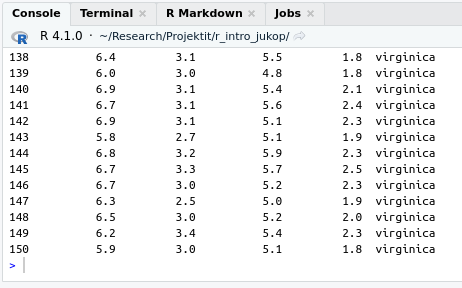
\includegraphics{files/02-data_types/iris_print_data.png}

\begin{Shaded}
\begin{Highlighting}[]
\CommentTok{\# Print 6 first rows of iris data}
\FunctionTok{head}\NormalTok{(iris)}
\end{Highlighting}
\end{Shaded}

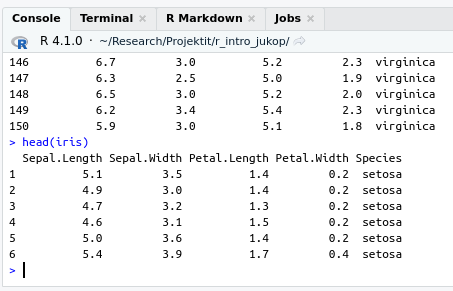
\includegraphics{files/02-data_types/iris_print_head_data.png}

\begin{Shaded}
\begin{Highlighting}[]
\CommentTok{\# You can also define the number of rows to print}
\FunctionTok{head}\NormalTok{(iris,}\DecValTok{2}\NormalTok{)}
\end{Highlighting}
\end{Shaded}

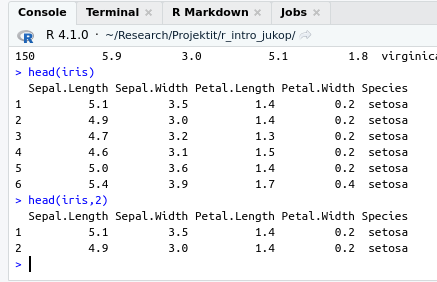
\includegraphics{files/02-data_types/iris_print_head2_data.png}

\hypertarget{extra-taulukko-ja-lista}{%
\section{Extra: Taulukko ja lista}\label{extra-taulukko-ja-lista}}

Taulukoita ja listoja ei perus data-analyysiä toteutettaessa yleensä tarvita. Lue kuitenkin seuraava, jotta saat yleiskäsityksen mihin niitä tarvitaan. Voit myös palata perehtymään taulukoihin ja listoihin myöhemmin koska tahansa.

\hypertarget{array}{%
\subsection{Taulukko}\label{array}}

Kuten alussa todettiin, taulukot (array) ovat hyvin harvinaisia, joten niihin ei kannata tällä kurssilla keskittyä. Niitä kuitenkin tarvitaan joidenkin tehtävien tekemiseen, joten tässä on hyvin lyhyt oppimäärä taulukoista.

Taulukot ovat matriisien kaltaisia, mutta taulukossa voi olla yli kaksi ulottuvuutta. Oikeastaan matriisit ovat kaksiulotteisia taulukoita. Alla on esimerkki 3-ulotteisesta taulukosta, jota voi ajatella ``peräkkäin'' olevina matriiseina. Alla on kuva 1-ulotteisesta taulukosta eli vektorista, 2-ulotteisesta taulukosta eli matriisista ja 3-ulotteisesta taulukosta.

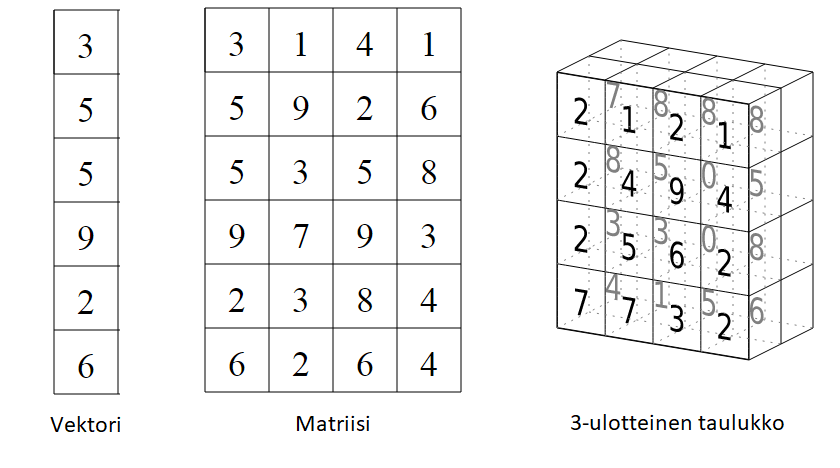
\includegraphics{files/array.png}

Taulukkoja luodaan matriisien tapaan funktiolla \texttt{array}. Toisin kuin matriisien tapauksessa, \texttt{array}-funktiolle pitää luetella sen kaikki ulottuvuudet vektorina. Alla oleva esimerkki luo 3-ulotteisen taulukon, jonka voi ajatella koostuvan kolmesta 4 x 2 matriisista.

\begin{Shaded}
\begin{Highlighting}[]
\NormalTok{my\_array }\OtherTok{\textless{}{-}} \FunctionTok{array}\NormalTok{(}\DecValTok{1}\SpecialCharTok{:}\DecValTok{24}\NormalTok{, }\AttributeTok{dim =} \FunctionTok{c}\NormalTok{(}\DecValTok{4}\NormalTok{, }\DecValTok{2}\NormalTok{, }\DecValTok{3}\NormalTok{))}
\NormalTok{my\_array}
\end{Highlighting}
\end{Shaded}

\begin{verbatim}
## , , 1
## 
##      [,1] [,2]
## [1,]    1    5
## [2,]    2    6
## [3,]    3    7
## [4,]    4    8
## 
## , , 2
## 
##      [,1] [,2]
## [1,]    9   13
## [2,]   10   14
## [3,]   11   15
## [4,]   12   16
## 
## , , 3
## 
##      [,1] [,2]
## [1,]   17   21
## [2,]   18   22
## [3,]   19   23
## [4,]   20   24
\end{verbatim}

Taulukoita indeksoidaan aivan kuten matriiseja, mutta jokaiselle ulottuvuudelle on annettava oma indeksi:

\begin{Shaded}
\begin{Highlighting}[]
\CommentTok{\# The first 2 rows of each "layer"}
\NormalTok{my\_array[}\DecValTok{1}\SpecialCharTok{:}\DecValTok{2}\NormalTok{, , ]}
\end{Highlighting}
\end{Shaded}

\begin{verbatim}
## , , 1
## 
##      [,1] [,2]
## [1,]    1    5
## [2,]    2    6
## 
## , , 2
## 
##      [,1] [,2]
## [1,]    9   13
## [2,]   10   14
## 
## , , 3
## 
##      [,1] [,2]
## [1,]   17   21
## [2,]   18   22
\end{verbatim}

\begin{Shaded}
\begin{Highlighting}[]
\CommentTok{\# Second column from last two layers}
\NormalTok{my\_array[, }\DecValTok{2}\NormalTok{, }\DecValTok{2}\SpecialCharTok{:}\DecValTok{3}\NormalTok{]}
\end{Highlighting}
\end{Shaded}

\begin{verbatim}
##      [,1] [,2]
## [1,]   13   21
## [2,]   14   22
## [3,]   15   23
## [4,]   16   24
\end{verbatim}

\hypertarget{list}{%
\subsection{Lista}\label{list}}

Listat ovat tärkeitä erityisesti silloin, kun aletaan toteuttamaan uusia toimintoja R-kieleen omien funktioiden avulla. Niin kauan kun valmiit R-funktiot riittävät, ei listoilla ole juuri käyttöä.

Lista (list) on vektorinkaltainen tietorakenne, jossa on järjestyksessä alkioita, jotka on mahdollisesti nimetty. Tärkeä ero vektoriin verrattuna on, että listan alkiot voivat olla erityyppisiä. Listoja luodaan \texttt{list}-funktiolla:

\begin{Shaded}
\begin{Highlighting}[]
\NormalTok{example\_list }\OtherTok{\textless{}{-}} \FunctionTok{list}\NormalTok{(}\FunctionTok{c}\NormalTok{(}\DecValTok{1}\NormalTok{, }\DecValTok{2}\NormalTok{, }\DecValTok{3}\NormalTok{),}
                     \FunctionTok{matrix}\NormalTok{(}\DecValTok{0}\NormalTok{, }\AttributeTok{nrow =} \DecValTok{3}\NormalTok{, }\AttributeTok{ncol =} \DecValTok{4}\NormalTok{),}
                     \StringTok{"list can include anything"}\NormalTok{)}
\NormalTok{example\_list}
\end{Highlighting}
\end{Shaded}

\begin{verbatim}
## [[1]]
## [1] 1 2 3
## 
## [[2]]
##      [,1] [,2] [,3] [,4]
## [1,]    0    0    0    0
## [2,]    0    0    0    0
## [3,]    0    0    0    0
## 
## [[3]]
## [1] "list can include anything"
\end{verbatim}

\begin{Shaded}
\begin{Highlighting}[]
\NormalTok{subject\_ids }\OtherTok{\textless{}{-}} \FunctionTok{c}\NormalTok{(}\StringTok{"ANKL"}\NormalTok{, }\StringTok{"PEPA"}\NormalTok{, }\StringTok{"DIPR"}\NormalTok{)}
\NormalTok{measurements }\OtherTok{\textless{}{-}} \FunctionTok{matrix}\NormalTok{(}\FunctionTok{c}\NormalTok{(}\DecValTok{1}\NormalTok{, }\FloatTok{2.5}\NormalTok{, }\DecValTok{3}\NormalTok{,}
                         \FloatTok{3.5}\NormalTok{, }\DecValTok{5}\NormalTok{, }\DecValTok{3}\NormalTok{,}
                         \FloatTok{2.3}\NormalTok{, }\DecValTok{3}\NormalTok{, }\FloatTok{1.6}\NormalTok{),}
                       \AttributeTok{nrow =} \DecValTok{3}\NormalTok{)}
\FunctionTok{colnames}\NormalTok{(measurements) }\OtherTok{\textless{}{-}} \FunctionTok{c}\NormalTok{(}\StringTok{"CRP"}\NormalTok{, }\StringTok{"HDL"}\NormalTok{, }\StringTok{"LDL"}\NormalTok{)}
\FunctionTok{rownames}\NormalTok{(measurements) }\OtherTok{\textless{}{-}}\NormalTok{ subject\_ids}
\CommentTok{\# List names can be given with or without quotes}
\NormalTok{study }\OtherTok{\textless{}{-}} \FunctionTok{list}\NormalTok{(}\AttributeTok{Subject\_ID =}\NormalTok{ subject\_ids,}
              \StringTok{"Measurements"} \OtherTok{=}\NormalTok{ measurements,}
              \AttributeTok{Study\_name =} \StringTok{"Blood tests"}\NormalTok{)}
\NormalTok{study}
\end{Highlighting}
\end{Shaded}

\begin{verbatim}
## $Subject_ID
## [1] "ANKL" "PEPA" "DIPR"
## 
## $Measurements
##      CRP HDL LDL
## ANKL 1.0 3.5 2.3
## PEPA 2.5 5.0 3.0
## DIPR 3.0 3.0 1.6
## 
## $Study_name
## [1] "Blood tests"
\end{verbatim}

Listoja ja niiden kaltaisia olioita käytetään R:ssä paljon. Listoihin on kätevä tallentaa erityyppistä tietoa, joka kuitenkin halutaan säilyttää yhtenä kokonaisuutena. Esimerkiksi yksinkertaisetkin tilastolliset mallit tuottavat paljon erilaista tietoa, joka tallennetaan listaan (tarkemmin listan kaltaiseen olioon, tästä lisää myöhemmin).

\hypertarget{listojen-alkioiden-kuxe4sittely}{%
\subsubsection{Listojen alkioiden käsittely}\label{listojen-alkioiden-kuxe4sittely}}

Listan alkioihin pääsee käsiksi kahdella eri tavalla: kaksoishakasulkeilla \texttt{{[}{[}{]}{]}} tai, jos lista on nimetty, dollarimerkillä \texttt{\$}:

\begin{Shaded}
\begin{Highlighting}[]
\CommentTok{\# By position}
\NormalTok{study[[}\DecValTok{2}\NormalTok{]]}
\end{Highlighting}
\end{Shaded}

\begin{verbatim}
##      CRP HDL LDL
## ANKL 1.0 3.5 2.3
## PEPA 2.5 5.0 3.0
## DIPR 3.0 3.0 1.6
\end{verbatim}

\begin{Shaded}
\begin{Highlighting}[]
\CommentTok{\# By name}
\NormalTok{study[[}\StringTok{"Subject\_ID"}\NormalTok{]]}
\end{Highlighting}
\end{Shaded}

\begin{verbatim}
## [1] "ANKL" "PEPA" "DIPR"
\end{verbatim}

\begin{Shaded}
\begin{Highlighting}[]
\CommentTok{\# Using dollar sign}
\NormalTok{study}\SpecialCharTok{$}\NormalTok{Study\_name}
\end{Highlighting}
\end{Shaded}

\begin{verbatim}
## [1] "Blood tests"
\end{verbatim}

Listaa voi indeksoida myös yksinkertaisilla hakasulkeilla. Tällöin palautetaan aina lista, eikä yksittäistä alkiota kuten aiemmin. Palautetaan ensiksi mieleen funktio \texttt{class}, joka palauttaa argumenttinsa luokan (class). Vektorin luokka vaihtelee vektorin sisällön mukaan: numeric = lukuja, character = merkkijonoja, logical = loogisia arvoja, jne. Listojen luokka on luonnollisesti list. R:ssä kaikki muuttujiin tallennettavat tiedot ovat olioita (object). R-olioilla on aina luokka, joka määrittää sen ominaisuudet. Esimerkiksi \texttt{print} ja \texttt{plot}-komennot toimivat eri tavalla riippuen niiden argumentin luokasta.

Tarkastellaan alla, mikä ero yksinkertaisilla ja kaksinkertaisilla hakasulkeilla on listan indeksoinnissa:

\begin{Shaded}
\begin{Highlighting}[]
\CommentTok{\# Returns a list of length one with the matrix as the only element}
\NormalTok{study[}\DecValTok{2}\NormalTok{]}
\end{Highlighting}
\end{Shaded}

\begin{verbatim}
## $Measurements
##      CRP HDL LDL
## ANKL 1.0 3.5 2.3
## PEPA 2.5 5.0 3.0
## DIPR 3.0 3.0 1.6
\end{verbatim}

\begin{Shaded}
\begin{Highlighting}[]
\FunctionTok{class}\NormalTok{(study[}\DecValTok{2}\NormalTok{])}
\end{Highlighting}
\end{Shaded}

\begin{verbatim}
## [1] "list"
\end{verbatim}

\begin{Shaded}
\begin{Highlighting}[]
\CommentTok{\# Returns the actual matrix}
\NormalTok{study[[}\DecValTok{2}\NormalTok{]]}
\end{Highlighting}
\end{Shaded}

\begin{verbatim}
##      CRP HDL LDL
## ANKL 1.0 3.5 2.3
## PEPA 2.5 5.0 3.0
## DIPR 3.0 3.0 1.6
\end{verbatim}

\begin{Shaded}
\begin{Highlighting}[]
\FunctionTok{class}\NormalTok{(study[[}\DecValTok{2}\NormalTok{]])}
\end{Highlighting}
\end{Shaded}

\begin{verbatim}
## [1] "matrix" "array"
\end{verbatim}

\begin{Shaded}
\begin{Highlighting}[]
\CommentTok{\# Dollar sign also returns the matrix}
\FunctionTok{class}\NormalTok{(study}\SpecialCharTok{$}\NormalTok{Measurements)}
\end{Highlighting}
\end{Shaded}

\begin{verbatim}
## [1] "matrix" "array"
\end{verbatim}

\begin{Shaded}
\begin{Highlighting}[]
\CommentTok{\# Single brackets works as subscripting just like with vectors}
\NormalTok{study[}\DecValTok{2}\SpecialCharTok{:}\DecValTok{3}\NormalTok{]}
\end{Highlighting}
\end{Shaded}

\begin{verbatim}
## $Measurements
##      CRP HDL LDL
## ANKL 1.0 3.5 2.3
## PEPA 2.5 5.0 3.0
## DIPR 3.0 3.0 1.6
## 
## $Study_name
## [1] "Blood tests"
\end{verbatim}

\hypertarget{alkion-lisuxe4ys-listaan-ja-listojen-yhdistuxe4minen}{%
\subsubsection{Alkion lisäys listaan ja listojen yhdistäminen}\label{alkion-lisuxe4ys-listaan-ja-listojen-yhdistuxe4minen}}

Yksittäisen alkion voi lisätä listaan sijoittamalla listan johonkin indeksiin tai nimeen uusi arvo (indeksin pitää olla yhtä suurempi kuin listan pituus). HUOM! Listan alkio voi myös itse olla lista (sisäkkäinen lista = nested list).

\begin{Shaded}
\begin{Highlighting}[]
\CommentTok{\# Add a character matrix as the fourth element of study}
\NormalTok{study[[}\DecValTok{4}\NormalTok{]] }\OtherTok{\textless{}{-}} \FunctionTok{matrix}\NormalTok{(}\FunctionTok{c}\NormalTok{(}\StringTok{"CPR"}\NormalTok{, }\StringTok{"HDL"}\NormalTok{, }\StringTok{"LDL"}\NormalTok{,}
                       \StringTok{"C{-}reactive protein"}\NormalTok{, }\StringTok{"High{-}density lipoprotein"}\NormalTok{,}
                       \StringTok{"Low{-}density lipoprotein"}\NormalTok{),}
                     \AttributeTok{ncol =} \DecValTok{2}\NormalTok{)}
\CommentTok{\# An element of a list can also be a list}
\NormalTok{study[[}\StringTok{"professional"}\NormalTok{]] }\OtherTok{\textless{}{-}} \FunctionTok{list}\NormalTok{(}\AttributeTok{name =} \FunctionTok{c}\NormalTok{(}\StringTok{"John H. Watson"}\NormalTok{),}
                                \AttributeTok{position =} \StringTok{"Medical doctor"}\NormalTok{,}
                                \AttributeTok{age =} \DecValTok{45}\NormalTok{)}
\NormalTok{study}
\end{Highlighting}
\end{Shaded}

\begin{verbatim}
## $Subject_ID
## [1] "ANKL" "PEPA" "DIPR"
## 
## $Measurements
##      CRP HDL LDL
## ANKL 1.0 3.5 2.3
## PEPA 2.5 5.0 3.0
## DIPR 3.0 3.0 1.6
## 
## $Study_name
## [1] "Blood tests"
## 
## [[4]]
##      [,1]  [,2]                      
## [1,] "CPR" "C-reactive protein"      
## [2,] "HDL" "High-density lipoprotein"
## [3,] "LDL" "Low-density lipoprotein" 
## 
## $professional
## $professional$name
## [1] "John H. Watson"
## 
## $professional$position
## [1] "Medical doctor"
## 
## $professional$age
## [1] 45
\end{verbatim}

\begin{Shaded}
\begin{Highlighting}[]
\CommentTok{\# Note that the fourth element has no name}
\FunctionTok{names}\NormalTok{(study)}
\end{Highlighting}
\end{Shaded}

\begin{verbatim}
## [1] "Subject_ID"   "Measurements" "Study_name"   ""             "professional"
\end{verbatim}

Listoja voi yhdistää vektorien tapaan \texttt{c}-funktiolla:

\begin{Shaded}
\begin{Highlighting}[]
\CommentTok{\# Concatenate two vectors}
\NormalTok{vector1 }\OtherTok{\textless{}{-}} \FunctionTok{c}\NormalTok{(}\DecValTok{3}\NormalTok{, }\DecValTok{6}\NormalTok{, }\DecValTok{5}\NormalTok{)}
\NormalTok{vector2 }\OtherTok{\textless{}{-}} \FunctionTok{c}\NormalTok{(}\DecValTok{1}\NormalTok{, }\DecValTok{2}\NormalTok{, }\DecValTok{3}\NormalTok{)}
\FunctionTok{c}\NormalTok{(vector1, vector2)}
\end{Highlighting}
\end{Shaded}

\begin{verbatim}
## [1] 3 6 5 1 2 3
\end{verbatim}

\begin{Shaded}
\begin{Highlighting}[]
\NormalTok{list1 }\OtherTok{\textless{}{-}} \FunctionTok{list}\NormalTok{(}\AttributeTok{vector =}\NormalTok{ vector1,}
              \AttributeTok{name =} \StringTok{"list1"}\NormalTok{)}
\NormalTok{list2 }\OtherTok{\textless{}{-}}\NormalTok{ study[}\DecValTok{1}\SpecialCharTok{:}\DecValTok{2}\NormalTok{]}
\CommentTok{\# Concatenate three lists, names stay the same}
\FunctionTok{c}\NormalTok{(list1, list2, }\FunctionTok{list}\NormalTok{(}\AttributeTok{first\_element =} \StringTok{"A"}\NormalTok{, }\AttributeTok{second =} \StringTok{"B"}\NormalTok{))}
\end{Highlighting}
\end{Shaded}

\begin{verbatim}
## $vector
## [1] 3 6 5
## 
## $name
## [1] "list1"
## 
## $Subject_ID
## [1] "ANKL" "PEPA" "DIPR"
## 
## $Measurements
##      CRP HDL LDL
## ANKL 1.0 3.5 2.3
## PEPA 2.5 5.0 3.0
## DIPR 3.0 3.0 1.6
## 
## $first_element
## [1] "A"
## 
## $second
## [1] "B"
\end{verbatim}

\hypertarget{reading_data}{%
\chapter{Datan lukeminen}\label{reading_data}}

Tässä osiossa tutustutaan datan sisään lukemiseen ja sisäänluetun datan tarkistamiseen. Tähän mennessä kaikki kurssilla käsitelty data on luotu R:ssä. Useimmiten R:llä käsiteltävä data on kuitenkin tallennettu tiedostoon, joka on luotu jollain ohjelmalla tai kirjattu esim. Excelissä.

Tässä esitellyt funktiot lukevat erilaisia tiedostoja, mutta kaikki palauttavat datakehikon. Datakehikko sopii aineiston käsittelyyn hyvin, sillä siihen voi tallentaa niin numeerisia kuin tekstimuotoisia muuttujia. Voit tarvittessa kerrata datakehikon toimintaa \protect\hyperlink{data-frame}{datakehikko}-kappaleesta.

Lopussa käydään myös läpi tapoja lukea taulukkolaskenta- (Excel), SPSS- ja SAS-tiedostoja. Näitä tiedostoja ei käsitellä kurssin tehtävissä, mutta on hyvä tietää, että niitä voi lukea R:ään suoraan muuttamatta niitä ensin johonkin toiseen muotoon.

\hypertarget{hakemistopolut-ja-tiedostopuxe4uxe4tteet}{%
\section{Hakemistopolut ja tiedostopäätteet}\label{hakemistopolut-ja-tiedostopuxe4uxe4tteet}}

\hypertarget{hakemistopolut}{%
\subsection{Hakemistopolut}\label{hakemistopolut}}

Jotta aineiston lataus tiedostosta onnistuu, tulee käyttäjän olla tietoinen siitä, missä hakemistopolussa eli kansiossa R työskentelee lataushetkellä. R:llä on siis koko ajan jokin hakemistopolku, johon se viittaa. R:n käyttämän hakemistopolun saat selville komennolla \texttt{getwd()}.

\begin{Shaded}
\begin{Highlighting}[]
\FunctionTok{getwd}\NormalTok{()}
\end{Highlighting}
\end{Shaded}

\begin{verbatim}
[1] "C:/Users/jukop/Documents"
\end{verbatim}

Minulla näyttäisi siltä, että R on oletuksena hakemistossa C:/Users/jukop/Documents. Jos olen purkanut kurssilla tarvittavan datasets.zip -tiedoston aineistot kansioon \texttt{C:/Users/jukop/Documents/datasets}, niin minun kannattaa vaihtaa R käyttämään kyseistä hakemistoa. Se tapahtuu näin:

\begin{Shaded}
\begin{Highlighting}[]
\FunctionTok{setwd}\NormalTok{(}\StringTok{"C:/Users/jukop/Documents/datasets"}\NormalTok{)}
\end{Highlighting}
\end{Shaded}

\texttt{setwd} ei tulosta mitään, jos kansion vaihtaminen onnistuu. Voit vielä \texttt{getwd()}-komennolla uudelleen tarkastaa, että hakemisto todella vaihtui.
\textbf{\emph{Vinkki!}} Ellet tiedä mikä on tarkka hakemistopolku, johon olet purkanut tiedostot, niin se onnistuu klikkaamalla Windowsissa tiedostoselaimen osoiteriviä. Voit kopioida hakemistopolun siitä, mutta vaihda kuitenkin kenoviivat (\texttt{\textbackslash{}}) kauttaviivoiksi (\texttt{/}). Kenoviivoilla on R:ssä erityismerkitys merkkijonoissa, joten ne eivät kelpaa sellaisenaan. Kaksinkertainen kenoviiva (\texttt{\textbackslash{}\textbackslash{}}) toimisi myös.
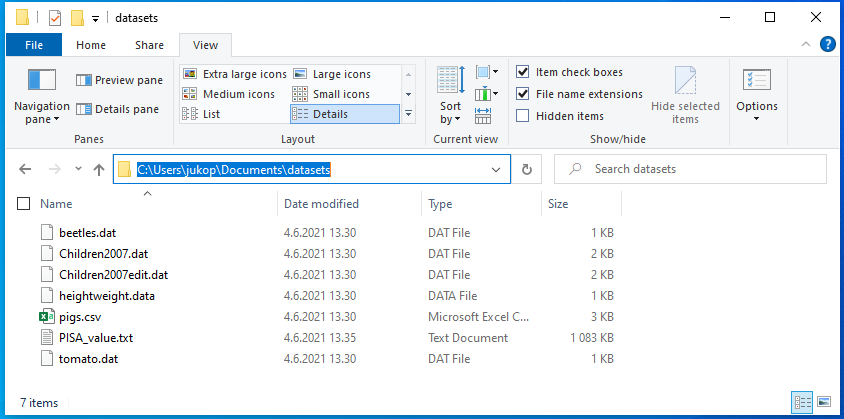
\includegraphics{files/03-reading_data/windows_show_file_path2.png}

\hypertarget{tiedostopuxe4uxe4tteet}{%
\subsection{Tiedostopäätteet}\label{tiedostopuxe4uxe4tteet}}

Windows ei oletuksena nykyisin näytä tiedostopäätteitä. Ne kannattaakin asettaa näkymään tiedostoselaimen avulla. Kyseinen asetus löytyy tiedostoselaimen View-välilehdeltä kohdasta Show/Hide valinta File extensions. Merkitse kyseinen kohta valituksi, jolloin näet tiedostopäätteet, kuten kuvassa. Nyt on helppoa käsittää, kun opettaja puhuu CSV-tiedostoista, että niiden tiedostopääte on .csv.
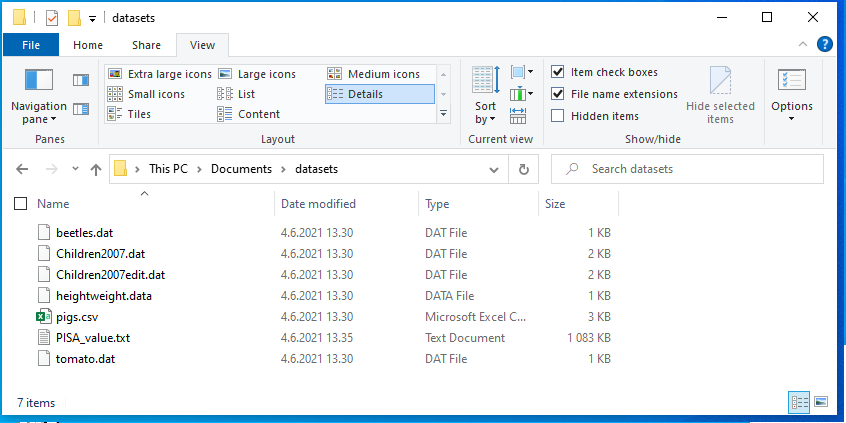
\includegraphics{files/03-reading_data/windows_show_file_extensions2.png}

\hypertarget{tekstitiedostot}{%
\section{Tekstitiedostot}\label{tekstitiedostot}}

Tekstitiedosto tarkoittaa tässä tapauksessa tiedostoa, joka ei sisällä tekstin lisäksi mitään muuta, kuten erilaisia muotoilutietoja. Tekstitiedostojen yleisimmät tiedostopäätteet ovat .txt ja .csv (comma separated value). Esim. Excelin .xlsx-tiedostot tai Wordin .docx-tiedostot eivät ole tekstitiedostoja, koska niissä on paljon muutakin tietoa tekstin lisäksi.

\hypertarget{read.table}{%
\subsection{read.table}\label{read.table}}

Kun dataa tallennetaan tekstitiedostoon, tiedoston ensimmäisellä rivillä ovat usein sarakkeiden nimet, ja seuraavilla riveillä mahdollisesti rivin nimi, ja sitten sarakkeiden arvot. Jokaisen kentän tulee olla erotettu samalla merkillä (field separator character). Yleisiä erotinmerkkejä ovat sarkain eli tab, välilyönti ja pilkku. Alla olevassa esimerkissä on neljältä kuvitteelliselta koehenkilöltä mitattu puna-vihervärisokeuteen liitettyjen geenien OPN1LW ja OPN1MW ilmentymistasot (lukuarvot ovat allekirjoittaneen hihasta). Tässä eri arvot on erotettu sarkaimella.

\begin{verbatim}
Subject_ID  OPN1LW  OPN1MW
ANKL    11264   12365
DIPR    10636   12725
PEPA    5630    13248
BRWA    8294    13060
\end{verbatim}

Tämä data löytyy myös oheisesta tiedostosta \texttt{gene\_data.txt}. Tekstitiedostot voi lukea sisään funktiolla \texttt{read.table}, jolla on tiedoston polun (file path) lisäksi monta muutakin argumenttia, joista tärkeimmät ovat:

\begin{itemize}
\tightlist
\item
  \texttt{header}: looginen arvo (TRUE/FALSE), jolla kerrotaan funktiolle, onko ensimmäisellä rivillä sarakkeiden nimet vai ei
\item
  \texttt{sep}: erotinmerkki, jolla muuttujien arvot on eroteltu
\item
  \texttt{dec}: desimaalierotin eli desimaalilukujen merkki, jolla desimaalit on eroteltu. Tämä on tärkeä lähinnä suomalaisille, koska Suomessa desimaalierotin on jostain syystä pilkku, eikä piste kuten useimmissa muissa maissa.
\end{itemize}

Luetaan edellisen esimerkin data R:ään data frameksi:

\begin{Shaded}
\begin{Highlighting}[]
\NormalTok{gene\_data }\OtherTok{\textless{}{-}} \FunctionTok{read.table}\NormalTok{(}\StringTok{"gene\_data.txt"}\NormalTok{, }\AttributeTok{header =} \ConstantTok{TRUE}\NormalTok{)}
\NormalTok{gene\_data}
\end{Highlighting}
\end{Shaded}

\begin{verbatim}
##   Subject_ID OPN1LW OPN1MW
## 1       ANKL  11264  12365
## 2       DIPR  10636  12725
## 3       PEPA   5630  13248
## 4       BRWA   8294  13060
\end{verbatim}

Yllä olevassa esimerkissä ei määritelty erikseen erotinmerkkiä, jolloin erotinmerkiksi tulkitaan kaikki tyhjä tila (white space) eli välilyönnit, sarkaimet jne. Halutessaan erotinmerkin voi myös asettaa. Jos erotinmerkki on sarkain, tulee asettaa \texttt{sep\ =\ "\textbackslash{}t"}

\begin{Shaded}
\begin{Highlighting}[]
\NormalTok{gene\_data }\OtherTok{\textless{}{-}} \FunctionTok{read.table}\NormalTok{(}\StringTok{"gene\_data.txt"}\NormalTok{, }\AttributeTok{sep =} \StringTok{"}\SpecialCharTok{\textbackslash{}t}\StringTok{"}\NormalTok{, }\AttributeTok{header =} \ConstantTok{TRUE}\NormalTok{)}
\NormalTok{gene\_data}
\end{Highlighting}
\end{Shaded}

\begin{verbatim}
##   Subject_ID OPN1LW OPN1MW
## 1       ANKL  11264  12365
## 2       DIPR  10636  12725
## 3       PEPA   5630  13248
## 4       BRWA   8294  13060
\end{verbatim}

Kuten yllä huomattiin, sarkain erotinmerkkinä merkataan \texttt{"\textbackslash{}t"}, eikä lainausmerkeillä, joiden sisään laitettaisiin tyhjää tilaa sarkainnäppäimellä. Tämä on yksi esimerkki koodinvaihtomerkin (escape character) \texttt{\textbackslash{}} käytöstä. R:ssä ja ohjelmointikielissä ylipäätään kenoviiva toimii koodinvaihtomerkkinä, eli sitä ei käsitellä kuin muita merkkejä, vaan se muuttaa seuraavan merkin toimintaa. Usein tämä tarkoittaa sitä, että kenoviivan avulla merkataan sarkainta, rivinvaihtoa (newline, \texttt{\textbackslash{}n}) ja muita erikoismerkkejä. Koodinvaihtomerkin käyttöä ei tarvitse osata tämän enempää, mutta se esitellään tässä, koska se aiheuttaa ongelmia Windowsin käyttäjille.

Windowsin tiedostopoluissa kansioiden välissä on kenoviiva, kun taas Mac- ja Linux-järjestelmissä käytetään kauttaviivaa \texttt{/}. Koska R:ssä kenoviiva on koodinvaihtomerkki, niin helpoin tapa on käyttää tiedostopoluissa Macin ja Linuxien tyyliä. Jos taas halutaan lukea tiedosto R:ään käyttäen Windowsin tapaisia tiedostopolkuja, kenoviivat \texttt{\textbackslash{}} pitää kirjoittaa kahteen kertaan eli \texttt{\textbackslash{}\textbackslash{}}, jotta R tulkitsee polun oikein. Tällöin ensimmäinen kenoviiva kertoo, että toinen kenoviiva on aito kenoviiva, eikä koodinvaihtomerkki.

Luetaan seuraavaksi sisään data-hakemistossa oleva tiedosto tooth\_growth.csv, joka sisältää dataa tutkimuksesta c-vitamiinin vaikutuksesta hampaiden kasvuun marsuilla. .csv-tiedostopääte tulee sanoista comma separated value, eli tiedostossa arvot ovat eroteltu pilkulla. Asetetaan siis sep-argumentiksi ``,''. Tämä tiedosto sisältää myös rivien nimet ensimmäisessä sarakkeessa. Tämä voidaan kertoa \texttt{read.table}-funktiolle argumentilla row.names, jonka arvoksi voi asettaa sarakkeen numeron, josta rivien nimet napataan.

\begin{Shaded}
\begin{Highlighting}[]
\NormalTok{tooth }\OtherTok{\textless{}{-}} \FunctionTok{read.table}\NormalTok{(}\StringTok{"data/tooth\_growth.csv"}\NormalTok{, }\AttributeTok{header =} \ConstantTok{TRUE}\NormalTok{, }\AttributeTok{sep =} \StringTok{","}\NormalTok{, }\AttributeTok{row.names =} \DecValTok{1}\NormalTok{)}
\NormalTok{tooth}
\end{Highlighting}
\end{Shaded}

\begin{verbatim}
##     len supp dose
## 34  9.7   OJ  0.5
## 16 17.3   VC  1.0
## 55 24.8   OJ  2.0
## 44 26.4   OJ  1.0
## 58 27.3   OJ  2.0
## 26 32.5   VC  2.0
## 14 17.3   VC  1.0
## 60 23.0   OJ  2.0
## 15 22.5   VC  1.0
## 9   5.2   VC  0.5
\end{verbatim}

Tutkimuksessa marsuille annettiin C-vitamiinia eri annoksina (dose, mitattu milligrammoina), joko appelsiinimehussa (OJ) tai askorbiinihappona (VC), ja mitattiin odontoblastien (hammasluun emosolu) pituus (len).

\hypertarget{read.csv}{%
\subsection{read.csv}\label{read.csv}}

.csv-tiedostot ovat niin yleisiä, että niiden lukemiseen on oma funktio: \texttt{read.csv}, joka on käytännössä sama funktio kuin \texttt{read.table}, mutta parametrien oletusarvot ovat erilaiset, niin että \texttt{read.csv(file)} \textasciitilde{} \texttt{read.table(file,\ header\ =\ TRUE,\ sep\ =\ ","))}.

\begin{Shaded}
\begin{Highlighting}[]
\NormalTok{tooth }\OtherTok{\textless{}{-}} \FunctionTok{read.csv}\NormalTok{(}\StringTok{"data/tooth\_growth.csv"}\NormalTok{, }\AttributeTok{row.names =} \DecValTok{1}\NormalTok{)}
\NormalTok{tooth}
\end{Highlighting}
\end{Shaded}

\begin{verbatim}
##     len supp dose
## 34  9.7   OJ  0.5
## 16 17.3   VC  1.0
## 55 24.8   OJ  2.0
## 44 26.4   OJ  1.0
## 58 27.3   OJ  2.0
## 26 32.5   VC  2.0
## 14 17.3   VC  1.0
## 60 23.0   OJ  2.0
## 15 22.5   VC  1.0
## 9   5.2   VC  0.5
\end{verbatim}

\hypertarget{read.csv2}{%
\subsubsection{read.csv2}\label{read.csv2}}

HUOM: Koska Suomessa pilkkua käytetään desimaalierottimena, kenttien rajaaminen pilkulla ei toimi. Käytännössä tämä näkyy siten, että suomenkielinen Excel tallentaa .csv-tiedosto oletuksena muodossa, jossa desimaalierottimena on pilkku ja kenttien välissä puolipilkku ``;''. Jos siis olet tallentanut Excelistä taulukon .csv-muotoon ja sen lukeminen R:ään aiheuttaa hankaluuksia, kyse on todennäköisesti erotinmerkistä. Onneksi R:ssä on valmiina funktio \texttt{read.csv2}, joka osaa lukea puolipilkulliset .csv-tiedostot oikein.

\hypertarget{datakehikon-tarkastelu}{%
\section{Datakehikon tarkastelu}\label{datakehikon-tarkastelu}}

Kun data on luettu sisään R:ään, kannattaa aina tarkistaa, että kaikki data on luettu oikein. Tässä muutama vinkki datakehikon tutkimiseen, joista osaa käsiteltiin jo \protect\hyperlink{data-frame}{datakehikko}-kappaleessa:

\texttt{dim} antaa data framen dimensiot, eli rivien ja sarakkeiden määrän.\\
\texttt{View} avaa data framen erilliseen ikkunaan, jossa sitä voi tarkastella. Suositellaan vain pienemmille data frameille
\texttt{str} kertoo rivien ja sarakkeiden määrät sekä kaikkien sarakkeiden luokat. Kätevä tapa tarkistaa mm. että lukuja sisältävät sarakkeet eivät ole vahingossa muuttuneet merkkijonoiksi.
\texttt{table} on kätevä kategoristen sarakkeiden tutkimiseen. Se kertoo, kuinka monta havaintoa muuttujan arvoilla on. \texttt{table} voi ottaa vastaan myös kaksi kategorista muuttujaa, ja laskee jokaiselle muuttujien arvojen yhdistelmälle havaintojen lukumäärän.

Katsotaan, mitä \texttt{str} kertoo juuri lukemastamme tooth-datasta.

\begin{Shaded}
\begin{Highlighting}[]
\FunctionTok{str}\NormalTok{(tooth)}
\end{Highlighting}
\end{Shaded}

\begin{verbatim}
## 'data.frame':    10 obs. of  3 variables:
##  $ len : num  9.7 17.3 24.8 26.4 27.3 32.5 17.3 23 22.5 5.2
##  $ supp: chr  "OJ" "VC" "OJ" "OJ" ...
##  $ dose: num  0.5 1 2 1 2 2 1 2 1 0.5
\end{verbatim}

Kuten näimme aiemmin, mukana on 10 havaintoa ja 3 muuttujaa. len ja dose ovat luokkaa numeric eli desimaalilukuja, ja supp on luokkaa factor. Factor-tietotyyppiä käsitellään enemmän lineaaristen mallien yhteydessä, mutta sillä merkitään usein kategorisia muuttujia.

Lasketaan seuraavaksi, kuinka monelle marsulle annettiin appelsiinimehua ja kuinka monelle askorbiinihappoa.

\begin{Shaded}
\begin{Highlighting}[]
\FunctionTok{table}\NormalTok{(tooth}\SpecialCharTok{$}\NormalTok{supp)}
\end{Highlighting}
\end{Shaded}

\begin{verbatim}
## 
## OJ VC 
##  5  5
\end{verbatim}

Kumpaakin annostelutapaa käytettiin siis viisi kertaa. Voimme myös selvittää, miten eri annokset jakautuvat annostelutavan suhteen:

\begin{Shaded}
\begin{Highlighting}[]
\FunctionTok{table}\NormalTok{(tooth}\SpecialCharTok{$}\NormalTok{supp, tooth}\SpecialCharTok{$}\NormalTok{dose)}
\end{Highlighting}
\end{Shaded}

\begin{verbatim}
##     
##      0.5 1 2
##   OJ   1 1 3
##   VC   1 3 1
\end{verbatim}

Appelsiinimehuna annettiin siis 0.5 mg ja 1 mg annoksia kumpaakin 1 kappale, ja 2 mg annoksia 3 kappaletta.

\hypertarget{rn-sisuxe4uxe4nrakennetut-datasetit}{%
\subsection{R:n sisäänrakennetut datasetit}\label{rn-sisuxe4uxe4nrakennetut-datasetit}}

R:ssä on monta sisäänrakennettua (built-in) datasettiä. Näitä on kätevää käyttää nopeaan testaamiseen, ja ne vilahtelevatkin usein R-oppaissa. Esimerkiksi aikaisempi odontoblastien pituuksia sisältävä datasettimme on oikeastaan pieni otos R:n sisäisestä datasetistä ToothGrowth.

R:n sisäiset datasetit ovat koko ajan käytettävissä, vaikka ne eivät näy RStudion ympäristössä (Environment). Voimme esimerkiksi katsoa, millainen rakenne kokonaisella ToothGroth-datasetillä on:

\begin{Shaded}
\begin{Highlighting}[]
\FunctionTok{str}\NormalTok{(ToothGrowth)}
\end{Highlighting}
\end{Shaded}

\begin{verbatim}
## 'data.frame':    60 obs. of  3 variables:
##  $ len : num  4.2 11.5 7.3 5.8 6.4 10 11.2 11.2 5.2 7 ...
##  $ supp: Factor w/ 2 levels "OJ","VC": 2 2 2 2 2 2 2 2 2 2 ...
##  $ dose: num  0.5 0.5 0.5 0.5 0.5 0.5 0.5 0.5 0.5 0.5 ...
\end{verbatim}

R:n datasettejä voi käyttää moneen eri tarkoitukseen, kuten datan visualisoinnin tai tilastollisten toimenpiteiden testaamiseen. Listan kaikista R:n dataseteistä saa komennolla \texttt{data()}. Tarkempia tietoja datasetistä saa help-sivulta kuten funktioden tapauksessa, esimerkiksi \texttt{?ToothGrowth}

\hypertarget{muut-tiedostot}{%
\section{Muut tiedostot}\label{muut-tiedostot}}

\hypertarget{excel}{%
\subsection{Excel}\label{excel}}

Excelin käyttämiä .xlsx-tiedostoja voi lukea suoraan R:ään, vaikka jossain netissä olevissa ohjeissa suositellaan niiden muuntamista ensin .csv-muotoon. Tätä varten pitää asentaa \textbf{readxl}-paketti, minkä voi tehdä RStudion Packages-valikoksta tai suoraan komennolla \texttt{install.packages("readxl")}. Paketin funktiolla \texttt{read\_xlsx()} voi lukea sisään .xlsx-tiedostoja, tai yksikkäitisä taulukon sivuja. Excel-tiedostojen kirjoittamiseen löytyy myös vastaava paketti \textbf{writexl}.

Vaihtoehtoinen paketti Excel-tiedostojen lukemiseen on \textbf{openxlsx}, jolla voi sekä lukea että kirjoittaa .xlsx-tiedostoja, mutta se on tyypillisesti hitaampi \emph{readxl} ja \emph{writexl} paketteihin verattuna.

\hypertarget{spss}{%
\subsection{SPSS}\label{spss}}

Eri tutkimusryhmissä dataa säilytetään usein SPSS-tiedostoissa (.sav). SPSS-tiedostojen käsittelyyn voi käyttää \textbf{haven}-paketin funktioita \texttt{read\_sav} ja \texttt{write\_sav}. \textbf{haven}-paketti sisältää myös funktiot Stata- ja SAS-tiedostoille.

SPSS-tiedostoja voi lukea myös \textbf{foreign}-paketin avulla, mutta ainakin minulla on parempia kokemuksia haven-paketista. \textbf{haven} on myös osa tidyverse-pakettikokoelmaa, joten oletan sen pysyvän hyvin ajan tasalla jatkossakin.

\hypertarget{data-wrangling}{%
\chapter{Datan muokkaaminen}\label{data-wrangling}}

Aineisto ei tyypillisesti ole valmiiksi oikeassa muodossa. Voi olla että halutaan esimerkiksi käyttää vain jotain osajoukkoa aineistosta. Tällöin tarvitaan komentoja aineiston muokkaamiseksi.

\textbf{Yleinen käytännön vinkki}
Aineiston muokkaaminen (data wrangling) on isojen tutkimusaineistojen kohdalla todella työlästä. Tällöin saatetaan joutua yhdistelemään aineistoja useista lähteistä, etsimään virheellisiä arvoja, muokkaamaan tekstimuotoisia (character) muuttujia eri muotoon ym. Mikäli halutaan muokata tekstimuotoisia vektoreita eri muotoon, niin ne kannattaa muuttaa faktoriksi vasta lopuksi, sillä muuttujan ei ole yleensä tarpeellista olla faktorimuodossa aineistoja muokatessa. Faktorit ovat tyypillisesti tarpeen vasta kun aineistoa aletaan todella analysoimaan.

\hypertarget{data-frame-wrangling}{%
\section{Uuden muuttujan tai rivin luonti datakehikkoon}\label{data-frame-wrangling}}

Uusi muuttuja voidaan luoda R:ssä joko perustuen aineiston muihin muuttujiin, tai muuttujan arvot voidaan syöttää vektorina aineistoon. Mikäli uusi muuttuja syötetään lukuina R-koodiin, tulee varmistua siitä, että havaintoja on sama määrä kuin aineistossa on rivejä. Muutoin aineisto tulee syötettyä virheellisesti ja tulokset eivät pidä paikkaansa.

Uuden sarakkeen luonti tapahtuu samalla tavalla kuin jo olemassa olevan sarakkeen muokkaaminen eli dollarisymbolilla, jossa dollarin jälkeen annetaan ensin uuden sarakkeen nimi ja tähän sijoitetaan halutut uuden muuttujan arvot.

\begin{Shaded}
\begin{Highlighting}[]
\CommentTok{\# evaluate the number of rows and columns}
\FunctionTok{dim}\NormalTok{(study\_data)}
\end{Highlighting}
\end{Shaded}

\begin{verbatim}
## [1] 8 3
\end{verbatim}

\begin{Shaded}
\begin{Highlighting}[]
\CommentTok{\# there are 8 rows}

\CommentTok{\# initiate a new variable called weight (imput data) with correct number of rows}
\NormalTok{study\_data}\SpecialCharTok{$}\NormalTok{weight }\OtherTok{\textless{}{-}} \FunctionTok{c}\NormalTok{(}\FloatTok{78.2}\NormalTok{, }\FloatTok{65.8}\NormalTok{, }\FloatTok{49.2}\NormalTok{, }\FloatTok{71.2}\NormalTok{, }\FloatTok{58.3}\NormalTok{, }\FloatTok{54.1}\NormalTok{, }\FloatTok{74.2}\NormalTok{, }\FloatTok{62.8}\NormalTok{)}

\CommentTok{\# calculate a new variable based on existing variables}
\NormalTok{study\_data}\SpecialCharTok{$}\NormalTok{height\_m }\OtherTok{\textless{}{-}}\NormalTok{ study\_data}\SpecialCharTok{$}\NormalTok{height }\SpecialCharTok{/} \DecValTok{100} \CommentTok{\# height as metres}
\NormalTok{study\_data}\SpecialCharTok{$}\NormalTok{BMI }\OtherTok{\textless{}{-}}\NormalTok{ study\_data}\SpecialCharTok{$}\NormalTok{weight }\SpecialCharTok{/}\NormalTok{ (study\_data}\SpecialCharTok{$}\NormalTok{height\_m}\SpecialCharTok{\^{}}\DecValTok{2}\NormalTok{)}
\NormalTok{study\_data}
\end{Highlighting}
\end{Shaded}

\begin{verbatim}
##   ID height gender weight height_m        BMI
## 1  1  189.8   male   78.2    1.898   21.70773
## 2  2  184.0 female   65.8    1.840   19.43526
## 3  3  173.8   male   49.2    1.738   16.28792
## 4  4  175.9   male   71.2    1.759   23.01168
## 5  5  169.0 female   58.3    1.690   20.41245
## 6  6  183.7   male   54.1    1.837   16.03168
## 7  7  181.8   male   74.2    1.818   22.44999
## 8  8   16.9 female   62.8    0.169 2198.80256
\end{verbatim}

\hypertarget{datakehikon-kuxe4sittely}{%
\subsection{Datakehikon käsittely}\label{datakehikon-kuxe4sittely}}

\begin{Shaded}
\begin{Highlighting}[]
\CommentTok{\# Subscripting with variable names}
\NormalTok{study\_data[, }\FunctionTok{c}\NormalTok{(}\StringTok{"height"}\NormalTok{, }\StringTok{"gender"}\NormalTok{)]}
\end{Highlighting}
\end{Shaded}

\begin{verbatim}
##   height gender
## 1  189.8   male
## 2  184.0 female
## 3  173.8   male
## 4  175.9   male
## 5  169.0 female
## 6  183.7   male
## 7  181.8   male
## 8   16.9 female
\end{verbatim}

\begin{Shaded}
\begin{Highlighting}[]
\CommentTok{\# Subscripting with brackets {-} as matrix (but I do not recommend this style!)}
\NormalTok{study\_data[, }\DecValTok{1}\SpecialCharTok{:}\DecValTok{2}\NormalTok{]}
\end{Highlighting}
\end{Shaded}

\begin{verbatim}
##   ID height
## 1  1  189.8
## 2  2  184.0
## 3  3  173.8
## 4  4  175.9
## 5  5  169.0
## 6  6  183.7
## 7  7  181.8
## 8  8   16.9
\end{verbatim}

\begin{Shaded}
\begin{Highlighting}[]
\CommentTok{\# Rownames and colnames}
\FunctionTok{colnames}\NormalTok{(study\_data)}
\end{Highlighting}
\end{Shaded}

\begin{verbatim}
## [1] "ID"       "height"   "gender"   "weight"   "height_m" "BMI"
\end{verbatim}

\begin{Shaded}
\begin{Highlighting}[]
\FunctionTok{names}\NormalTok{(study\_data)}
\end{Highlighting}
\end{Shaded}

\begin{verbatim}
## [1] "ID"       "height"   "gender"   "weight"   "height_m" "BMI"
\end{verbatim}

\begin{Shaded}
\begin{Highlighting}[]
\CommentTok{\# Individual columns can be accessed and added with dollar sign}
\CommentTok{\# Let\textquotesingle{}s say that we find out that the ID number 8 was typed in incorrectly. We can fix the entire height variables as follows}
\NormalTok{study\_data}\SpecialCharTok{$}\NormalTok{height }\OtherTok{\textless{}{-}} \FunctionTok{c}\NormalTok{(}\FloatTok{189.8}\NormalTok{, }\FloatTok{184.0}\NormalTok{, }\FloatTok{173.8}\NormalTok{, }\FloatTok{175.9}\NormalTok{, }\FloatTok{169.0}\NormalTok{, }\FloatTok{183.7}\NormalTok{, }\ConstantTok{NA}\NormalTok{, }\FloatTok{160.9}\NormalTok{)}
\NormalTok{study\_data}
\end{Highlighting}
\end{Shaded}

\begin{verbatim}
##   ID height gender weight height_m        BMI
## 1  1  189.8   male   78.2    1.898   21.70773
## 2  2  184.0 female   65.8    1.840   19.43526
## 3  3  173.8   male   49.2    1.738   16.28792
## 4  4  175.9   male   71.2    1.759   23.01168
## 5  5  169.0 female   58.3    1.690   20.41245
## 6  6  183.7   male   54.1    1.837   16.03168
## 7  7     NA   male   74.2    1.818   22.44999
## 8  8  160.9 female   62.8    0.169 2198.80256
\end{verbatim}

\begin{Shaded}
\begin{Highlighting}[]
\CommentTok{\# It would have been possible to change value of only one cell e.g. like this}
\NormalTok{study\_data}\SpecialCharTok{$}\NormalTok{height[}\DecValTok{8}\NormalTok{] }\OtherTok{\textless{}{-}} \FloatTok{161.9}
\NormalTok{study\_data}
\end{Highlighting}
\end{Shaded}

\begin{verbatim}
##   ID height gender weight height_m        BMI
## 1  1  189.8   male   78.2    1.898   21.70773
## 2  2  184.0 female   65.8    1.840   19.43526
## 3  3  173.8   male   49.2    1.738   16.28792
## 4  4  175.9   male   71.2    1.759   23.01168
## 5  5  169.0 female   58.3    1.690   20.41245
## 6  6  183.7   male   54.1    1.837   16.03168
## 7  7     NA   male   74.2    1.818   22.44999
## 8  8  161.9 female   62.8    0.169 2198.80256
\end{verbatim}

Uuden rivin lisäys datakehikkoon on hieman monimutkaisempaa kuin uuden rivin lisääminen matriisiin, sillä ensin pitää tehdä uusi datakehikko, jolla on samat sarakkeet kuin alkuperäisellä (samassa järjestyksessä), ja vasta sitten liittää se komennolla \texttt{rbind}. Käyttäjän tulee myös huolehtia siitä, että sarakkeet ovat samaa tyyppiä kuin alkuperäisessä datakehikossa.

\begin{Shaded}
\begin{Highlighting}[]
\NormalTok{new\_row }\OtherTok{\textless{}{-}} \FunctionTok{data.frame}\NormalTok{(}\AttributeTok{ID =} \DecValTok{11}\NormalTok{, }\AttributeTok{height =} \DecValTok{182}\NormalTok{, }\AttributeTok{gender =} \StringTok{"male"}\NormalTok{, }
                      \AttributeTok{weight =} \FloatTok{81.2}\NormalTok{, }\AttributeTok{height\_m =} \FloatTok{1.82}\NormalTok{, }\AttributeTok{BMI =} \FloatTok{81.2} \SpecialCharTok{/} \FloatTok{1.82}\SpecialCharTok{\^{}}\DecValTok{2}\NormalTok{)}
\FunctionTok{rbind}\NormalTok{(study\_data, new\_row)}
\end{Highlighting}
\end{Shaded}

\begin{verbatim}
##   ID height gender weight height_m        BMI
## 1  1  189.8   male   78.2    1.898   21.70773
## 2  2  184.0 female   65.8    1.840   19.43526
## 3  3  173.8   male   49.2    1.738   16.28792
## 4  4  175.9   male   71.2    1.759   23.01168
## 5  5  169.0 female   58.3    1.690   20.41245
## 6  6  183.7   male   54.1    1.837   16.03168
## 7  7     NA   male   74.2    1.818   22.44999
## 8  8  161.9 female   62.8    0.169 2198.80256
## 9 11  182.0   male   81.2    1.820   24.51395
\end{verbatim}

\hypertarget{osajoukkojen-valinta}{%
\section{Osajoukkojen valinta}\label{osajoukkojen-valinta}}

Aineistosta voi poimia osajoukon hakasulkujen avulla indeksoimalla. Osajoukon poimintaan tarvitaan usein vertailuoperattoreita, ja jos kriteerejä on useita, niin tarvitaan myös useita loogisia operaattoreita. Tarkemmin operaattoreita käsitellään luvussa \protect\hyperlink{loogiset-operaattorit}{Loogiset operaattorit}. Voit käyttää kyseisen osion taulukkoa apuna jo tässä osiossa.

\begin{Shaded}
\begin{Highlighting}[]
\CommentTok{\# Filter only females}
\NormalTok{study\_data[study\_data}\SpecialCharTok{$}\NormalTok{gender }\SpecialCharTok{==} \StringTok{"female"}\NormalTok{, ]}
\end{Highlighting}
\end{Shaded}

\begin{verbatim}
##   ID height gender weight height_m        BMI
## 2  2  184.0 female   65.8    1.840   19.43526
## 5  5  169.0 female   58.3    1.690   20.41245
## 8  8  161.9 female   62.8    0.169 2198.80256
\end{verbatim}

\begin{Shaded}
\begin{Highlighting}[]
\CommentTok{\# Filter individuals whose height is less than or equal to 175}
\NormalTok{study\_data[study\_data}\SpecialCharTok{$}\NormalTok{height }\SpecialCharTok{\textless{}=} \DecValTok{175}\NormalTok{, ]}
\end{Highlighting}
\end{Shaded}

\begin{verbatim}
##    ID height gender weight height_m        BMI
## 3   3  173.8   male   49.2    1.738   16.28792
## 5   5  169.0 female   58.3    1.690   20.41245
## NA NA     NA   <NA>     NA       NA         NA
## 8   8  161.9 female   62.8    0.169 2198.80256
\end{verbatim}

\begin{Shaded}
\begin{Highlighting}[]
\CommentTok{\# Filter individuals whose height is not missing and is less than or equal to 175}
\NormalTok{study\_data[}\SpecialCharTok{!}\FunctionTok{is.na}\NormalTok{(study\_data}\SpecialCharTok{$}\NormalTok{height) }\SpecialCharTok{\&}\NormalTok{ study\_data}\SpecialCharTok{$}\NormalTok{height }\SpecialCharTok{\textless{}=} \DecValTok{175}\NormalTok{, ]}
\end{Highlighting}
\end{Shaded}

\begin{verbatim}
##   ID height gender weight height_m        BMI
## 3  3  173.8   male   49.2    1.738   16.28792
## 5  5  169.0 female   58.3    1.690   20.41245
## 8  8  161.9 female   62.8    0.169 2198.80256
\end{verbatim}

\begin{Shaded}
\begin{Highlighting}[]
\CommentTok{\# Use multiple filter criteria}
\NormalTok{study\_data[study\_data}\SpecialCharTok{$}\NormalTok{height }\SpecialCharTok{\textless{}=} \DecValTok{175} \SpecialCharTok{\&}\NormalTok{ study\_data}\SpecialCharTok{$}\NormalTok{gender }\SpecialCharTok{==} \StringTok{"female"}\NormalTok{, ]}
\end{Highlighting}
\end{Shaded}

\begin{verbatim}
##   ID height gender weight height_m        BMI
## 5  5  169.0 female   58.3    1.690   20.41245
## 8  8  161.9 female   62.8    0.169 2198.80256
\end{verbatim}

\hypertarget{faktorit}{%
\section{Faktorit}\label{faktorit}}

R:n numeeriset vektorit ovat lähtökohtaisesti jatkuva-asteikollisia. Olet ehkä ihmetellytkin, miten kategorinen muuttuja määritellään. Kategorista muuttujaa sanotaan R:ssä faktoriksi. Numeerisen tai tekstimuotoisen muuttujan tai vektorin voi muuttaa faktori-muotoiseksi muuttujaksi \texttt{factor} -funktiolla.

\begin{Shaded}
\begin{Highlighting}[]
\CommentTok{\# Let\textquotesingle{}s change gender from character string to a factor and rename it as fgender}
\NormalTok{study\_data}\SpecialCharTok{$}\NormalTok{fgender }\OtherTok{\textless{}{-}} \FunctionTok{factor}\NormalTok{(study\_data}\SpecialCharTok{$}\NormalTok{gender)}

\CommentTok{\# Let\textquotesingle{}s now compare the printing of gender and fgender}
\NormalTok{study\_data}\SpecialCharTok{$}\NormalTok{gender}
\end{Highlighting}
\end{Shaded}

\begin{verbatim}
## [1] "male"   "female" "male"   "male"   "female" "male"   "male"   "female"
\end{verbatim}

\begin{Shaded}
\begin{Highlighting}[]
\NormalTok{study\_data}\SpecialCharTok{$}\NormalTok{fgender}
\end{Highlighting}
\end{Shaded}

\begin{verbatim}
## [1] male   female male   male   female male   male   female
## Levels: female male
\end{verbatim}

Huomataan, että faktori tulostaa faktorin tasot eli kaikkien mahdollisten luokkien nimet faktorin perässä: \texttt{Levels:\ female\ male}.

Usein vastaan tulee myös tilanne, jossa faktorin eri tasoja vastaavat kokonaislukuarvot, kuten tässä esimerkissä luvut 1, 2 ja 3. Tällaisessa tilanteessa faktorin tasojen merkitys on usein annettu jossain dokumenttitiedostossa. Tällöin faktorin tasot ja niiden kuvaukset (labels) tulee määrittää käsin.

\begin{Shaded}
\begin{Highlighting}[]
\CommentTok{\# Create a data for this example}
\NormalTok{wall\_dat }\OtherTok{\textless{}{-}} \FunctionTok{data.frame}\NormalTok{(}\AttributeTok{building\_ID =} \FunctionTok{c}\NormalTok{(}\DecValTok{1}\NormalTok{, }\DecValTok{2}\NormalTok{, }\DecValTok{3}\NormalTok{, }\DecValTok{4}\NormalTok{, }\DecValTok{5}\NormalTok{, }\DecValTok{6}\NormalTok{), }\AttributeTok{building\_material =} \FunctionTok{c}\NormalTok{(}\DecValTok{1}\NormalTok{, }\DecValTok{1}\NormalTok{, }\DecValTok{2}\NormalTok{, }\DecValTok{2}\NormalTok{, }\DecValTok{3}\NormalTok{, }\DecValTok{3}\NormalTok{))}

\CommentTok{\# Name is \textquotesingle{}building\_material\textquotesingle{} very long, I want to rename it}
\FunctionTok{names}\NormalTok{(wall\_dat) }\OtherTok{\textless{}{-}} \FunctionTok{c}\NormalTok{(}\StringTok{"building\_ID"}\NormalTok{, }\StringTok{"build\_mat"}\NormalTok{)}

\CommentTok{\# We know from some kind of documentation that 1 stands for "wood", 2 is "steel" and 3 is "brick".}
\NormalTok{wall\_dat}\SpecialCharTok{$}\NormalTok{fbuild\_mat }\OtherTok{\textless{}{-}} \FunctionTok{factor}\NormalTok{(wall\_dat}\SpecialCharTok{$}\NormalTok{build\_mat,}\AttributeTok{levels =} \FunctionTok{c}\NormalTok{(}\DecValTok{1}\NormalTok{, }\DecValTok{2}\NormalTok{, }\DecValTok{3}\NormalTok{), }\AttributeTok{labels =} \FunctionTok{c}\NormalTok{(}\StringTok{"wood"}\NormalTok{, }\StringTok{"steel"}\NormalTok{, }\StringTok{"brick"}\NormalTok{))}

\FunctionTok{str}\NormalTok{(wall\_dat)}
\end{Highlighting}
\end{Shaded}

\begin{verbatim}
## 'data.frame':    6 obs. of  3 variables:
##  $ building_ID: num  1 2 3 4 5 6
##  $ build_mat  : num  1 1 2 2 3 3
##  $ fbuild_mat : Factor w/ 3 levels "wood","steel",..: 1 1 2 2 3 3
\end{verbatim}

\hypertarget{factor-extra}{%
\section{Extra: Lääketutkimusesimerkki}\label{factor-extra}}

R:ssä on aiemmin nähtyjen numeric, character ja logical-vektorien lisäksi muitakin vektoriluokkia, tärkeimpänä näistä factor. Factor-vektoreihin tallennetaan kategorisia muuttujia, kuten tutkimuksessa määrättyjä ryhmiä, aikapisteitä tms. Luodaan esimerkiksi factor-vektori, jossa on kuvitteellisen lääketutkimuksen osallistujien ryhmätiedot:

\begin{Shaded}
\begin{Highlighting}[]
\NormalTok{groups }\OtherTok{\textless{}{-}} \FunctionTok{as.factor}\NormalTok{(}\FunctionTok{c}\NormalTok{(}\StringTok{"drug1"}\NormalTok{, }\StringTok{"drug2"}\NormalTok{, }\StringTok{"control"}\NormalTok{, }\StringTok{"drug1"}\NormalTok{, }\StringTok{"control"}\NormalTok{,}
                      \StringTok{"drug2"}\NormalTok{, }\StringTok{"drug2"}\NormalTok{, }\StringTok{"control"}\NormalTok{, }\StringTok{"control"}\NormalTok{, }\StringTok{"drug1"}\NormalTok{))}
\NormalTok{groups}
\end{Highlighting}
\end{Shaded}

\begin{verbatim}
##  [1] drug1   drug2   control drug1   control drug2   drug2   control control
## [10] drug1  
## Levels: control drug1 drug2
\end{verbatim}

Factoreita voi luoda muista vektoreista funktioilla \texttt{factor} tai \texttt{as.factor}. \texttt{as.factor} muuntaa vektorin automaattisesti ja nopeasti factoriksi, ja säilyttää myös jo valmiiksi factor-luokan vektorien tasojen järjestyksen (tästä lisää pian).

Kuten tulosteesta nähdään, factor-vektorin tulostus tulostaa factorin alkiot (HUOM: ei lainausmerkkejä) sekä factorin tasot. Factorit ovat pinnan alla kokonaisluku- eli integer-vektoreita, joissa on päällä ``kerros'', joka määrittää factorin tasot. Edellä nähty vektori groups näyttää siis tältä:

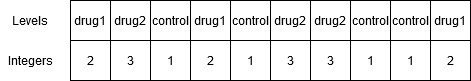
\includegraphics{files/05-statistics/factor.png}

Factorien tasoille annetaan siis lukuarvot ykkösestä eteenpäin. Oletuksena ensimmäinen taso eli taso 1 on aakkosissa ensimmäinen arvo, tai pienin lukuarvo jos factori tehdään numeerisista muuttujista. Lukuarvot saa näkyville muuntamalla factorin numeeriseksi vektoriksi:

\begin{Shaded}
\begin{Highlighting}[]
\FunctionTok{as.numeric}\NormalTok{(groups)}
\end{Highlighting}
\end{Shaded}

\begin{verbatim}
##  [1] 2 3 1 2 1 3 3 1 1 2
\end{verbatim}

Tasojen järjestyksen voi myös päättää itse. Tämä on tärkeää, sillä kuten pian nähdään, factorin ensimmäinen taso on monissa tilastollisissa testeissä ns. referenssitaso, johon muita tasoja verrataan. Usein esiintyvä tapaus ovat tutkimukset, joissa on ryhmät nimeltä case ja control. Koska case on aakkosissa ennen controllia, R käyttää oletuksen case-ryhmää referenssitasona, ja testaa miten control-ryhmä poikkeaa tästä tasosta, vaikka haluaisimme päinvastaisen tuloksen. Tasot voi itse määrittää näin:

\begin{Shaded}
\begin{Highlighting}[]
\NormalTok{study\_groups }\OtherTok{\textless{}{-}} \FunctionTok{factor}\NormalTok{(}\FunctionTok{c}\NormalTok{(}\StringTok{"case"}\NormalTok{, }\StringTok{"control"}\NormalTok{, }\StringTok{"control"}\NormalTok{, }\StringTok{"case"}\NormalTok{, }\StringTok{"case"}\NormalTok{),}
                       \AttributeTok{levels =} \FunctionTok{c}\NormalTok{(}\StringTok{"control"}\NormalTok{, }\StringTok{"case"}\NormalTok{))}
\NormalTok{study\_groups}
\end{Highlighting}
\end{Shaded}

\begin{verbatim}
## [1] case    control control case    case   
## Levels: control case
\end{verbatim}

Nyt tasot ovat oikeassa järjestyksessä!

Kuten aiemmin mainittiin, factoreita voi tehdä myös numeerisista vektoreista. HUOM: muista, että \texttt{as.numeric()} palauttaa factorin kokonaislukuarvot, ei alkuperäisiä lukuja. Alkuperäiset luvut saa käyttämällä ensin \texttt{as.character}-funktiota, joka muuttaa factorin tasot merkkijonovektoriksi.

\begin{Shaded}
\begin{Highlighting}[]
\NormalTok{time\_points }\OtherTok{\textless{}{-}} \FunctionTok{as.factor}\NormalTok{(}\FunctionTok{c}\NormalTok{(}\DecValTok{0}\NormalTok{, }\DecValTok{0}\NormalTok{, }\DecValTok{1}\NormalTok{, }\DecValTok{1}\NormalTok{, }\DecValTok{5}\NormalTok{, }\DecValTok{5}\NormalTok{, }\DecValTok{1}\NormalTok{, }\DecValTok{0}\NormalTok{, }\DecValTok{5}\NormalTok{))}
\NormalTok{time\_points}
\end{Highlighting}
\end{Shaded}

\begin{verbatim}
## [1] 0 0 1 1 5 5 1 0 5
## Levels: 0 1 5
\end{verbatim}

\begin{Shaded}
\begin{Highlighting}[]
\CommentTok{\# Probably not what you expect}
\FunctionTok{as.numeric}\NormalTok{(time\_points)}
\end{Highlighting}
\end{Shaded}

\begin{verbatim}
## [1] 1 1 2 2 3 3 2 1 3
\end{verbatim}

\begin{Shaded}
\begin{Highlighting}[]
\CommentTok{\# First to character, then to numeric}
\FunctionTok{as.numeric}\NormalTok{(}\FunctionTok{as.character}\NormalTok{(time\_points))}
\end{Highlighting}
\end{Shaded}

\begin{verbatim}
## [1] 0 0 1 1 5 5 1 0 5
\end{verbatim}

\hypertarget{statistics}{%
\chapter{Tunnusluvut}\label{statistics}}

Tunnusluvut (engl. statistics) ovat keskeinen osa tilastotiedettä. Tunnuslukujen avulla voidaan tiivistää ja tarkastella aineistoa. Tässä harjoittelemme tyypillisimpien tunnuslukujen laskemista aineistosta. Näitä tunnuslukuja voi sanoa myös empiirisiksi, koska ne on laskettu aineistosta.

\hypertarget{sijaintia-kuvaavat-tunnusluvut}{%
\section{Sijaintia kuvaavat tunnusluvut}\label{sijaintia-kuvaavat-tunnusluvut}}

\hypertarget{minimi-ja-maksimi}{%
\subsection{Minimi ja maksimi}\label{minimi-ja-maksimi}}

Minimi tarkoittaa aineiston pienintä arvoa kyseiselle muuttujalle. Maksimi on vastaavasti suurin arvo. Minimi ja maksimi ovat periaatteessa helppo laskea funktioiden \texttt{min} ja \texttt{max} avulla, mutta niihinkin liittyy pari pientä sudenkuoppaa. Funktiot \texttt{min} ja \texttt{max} hyväksyvät argumenteikseen vain numeerisia vektoreita.

\begin{Shaded}
\begin{Highlighting}[]
\NormalTok{dat\_for\_loc }\OtherTok{\textless{}{-}} \FunctionTok{c}\NormalTok{(}\SpecialCharTok{{-}}\FloatTok{1.25}\NormalTok{, }\SpecialCharTok{{-}}\FloatTok{4.1}\NormalTok{, }\FloatTok{1.16}\NormalTok{, }\SpecialCharTok{{-}}\FloatTok{3.05}\NormalTok{, }\FloatTok{4.17}\NormalTok{, }\FloatTok{0.73}\NormalTok{, }\SpecialCharTok{{-}}\FloatTok{3.14}\NormalTok{, }\FloatTok{3.39}\NormalTok{, }\SpecialCharTok{{-}}\FloatTok{2.55}\NormalTok{, }\FloatTok{0.4}\NormalTok{)}
\FunctionTok{min}\NormalTok{(dat\_for\_loc)}
\end{Highlighting}
\end{Shaded}

\begin{verbatim}
## [1] -4.1
\end{verbatim}

\begin{Shaded}
\begin{Highlighting}[]
\FunctionTok{max}\NormalTok{(dat\_for\_loc)}
\end{Highlighting}
\end{Shaded}

\begin{verbatim}
## [1] 4.17
\end{verbatim}

Joskus minimiä ja maksimia tarvitaan tilanteessa, jossa halutaan vaikkapa muuttaa kaikki negatiiviset arvot nolliksi (tai positiiviset, jos maksimi). Tämä onnistuu helpoiten funktioiden \texttt{pmin} ja \texttt{pmax} avulla. Samalla tapaa, jos halutaan kaikki lukua 1 pienemmät luvut muutettua luvuksi 1, niin tämä onnistuu vaihtamalla luku 0 lukuun 1.

\begin{Shaded}
\begin{Highlighting}[]
\CommentTok{\# We want to get rid of all values below 0 and make them 0}
\FunctionTok{pmin}\NormalTok{(dat\_for\_loc, }\DecValTok{0}\NormalTok{)}
\end{Highlighting}
\end{Shaded}

\begin{verbatim}
##  [1] -1.25 -4.10  0.00 -3.05  0.00  0.00 -3.14  0.00 -2.55  0.00
\end{verbatim}

\begin{Shaded}
\begin{Highlighting}[]
\CommentTok{\# Similar, but get rid of all values over 0}
\FunctionTok{pmax}\NormalTok{(dat\_for\_loc, }\DecValTok{0}\NormalTok{)}
\end{Highlighting}
\end{Shaded}

\begin{verbatim}
##  [1] 0.00 0.00 1.16 0.00 4.17 0.73 0.00 3.39 0.00 0.40
\end{verbatim}

\begin{Shaded}
\begin{Highlighting}[]
\CommentTok{\# We can do similar things to any limit, e.g. 1}
\FunctionTok{pmin}\NormalTok{(dat\_for\_loc, }\DecValTok{1}\NormalTok{)}
\end{Highlighting}
\end{Shaded}

\begin{verbatim}
##  [1] -1.25 -4.10  1.00 -3.05  1.00  0.73 -3.14  1.00 -2.55  0.40
\end{verbatim}

Funktiota \texttt{pmin} ja \texttt{pmax} voi käyttää vieläkin yleisemmässä muodossa antamalla yksittäisen lukuarvon sijasta vektorin. Näitä emme käsittele tässä, mutta kiinnostuneet voivat kokeilla lisää itse.

\hypertarget{keskiarvo}{%
\subsection{Keskiarvo}\label{keskiarvo}}

Keskiarvo saadaan laskemalla muuttujan kaikki havainnot yhteen ja jakamalla summa havaintojen määrällä. Esimerkiksi aineiston \(1,2,3,4\) keskiarvo on \((1+2+3+4)/4 = 2.5\). Keskiarvoa satunnaismuuttujan \(X\) havainnoille voidaan merkitä matemaattisesti seuraavasti
\[\overline{x} = \frac1n \sum_{i=1}^n x_i = \frac{x_1+x_2+\dots+x_n}{n},\]
missä merkintä \(\overline{x}\) tarkoittaa itse keskiarvoa, \(x_1,...,x_n\) ovat havaintoja ja \(n\) on havaintojen määrä.

Keskiarvo voidaan laskea helposti funktiolla \texttt{mean}.

\begin{Shaded}
\begin{Highlighting}[]
\NormalTok{tooth\_length }\OtherTok{\textless{}{-}}\NormalTok{ ToothGrowth}\SpecialCharTok{$}\NormalTok{len}
\FunctionTok{mean}\NormalTok{(tooth\_length)}
\end{Highlighting}
\end{Shaded}

\begin{verbatim}
## [1] 18.81333
\end{verbatim}

Mikäli muuttujassa on puuttuvia arvoja (\texttt{NA}) niin keskiarvoksi tulee oletusarvoisesti \texttt{NA}. Puuttuvat arvot voi jättää pois keskiarvon laskemisessa antamalla funktiolle lisäargumentiksi \texttt{na.rm\ =\ TRUE}.

\begin{Shaded}
\begin{Highlighting}[]
\CommentTok{\# Create some data}
\NormalTok{dat\_for\_mean }\OtherTok{\textless{}{-}} \FunctionTok{c}\NormalTok{(}\DecValTok{1}\NormalTok{, }\DecValTok{2}\NormalTok{, }\ConstantTok{NA}\NormalTok{, }\DecValTok{4}\NormalTok{)}
\CommentTok{\# Data with NA results mean with NA}
\FunctionTok{mean}\NormalTok{(dat\_for\_mean)}
\end{Highlighting}
\end{Shaded}

\begin{verbatim}
## [1] NA
\end{verbatim}

\begin{Shaded}
\begin{Highlighting}[]
\CommentTok{\# Leave NA{-}values out and calculate mean from the remaining ones}
\FunctionTok{mean}\NormalTok{(dat\_for\_mean, }\AttributeTok{na.rm =} \ConstantTok{TRUE}\NormalTok{)}
\end{Highlighting}
\end{Shaded}

\begin{verbatim}
## [1] 2.333333
\end{verbatim}

\hypertarget{mediaani}{%
\subsection{Mediaani}\label{mediaani}}

Mediaani ilmaisee aineiston keskimmäisen havainnon. Toisin sanoen puolet havainnoista on mediaania suurempia ja puolet mediaania pienempiä. Esimerkiksi aineiston \(1, 1, 2, 3, 5\) mediaani on \(2\). Jos aineistossa on parillinen määrä lukuja, otetaan kaksi keskimmäisä ja lasketaan ne yhteen ja jaetaan kahdella (keskiarvo). Aineiston \(3, 3, 5, 6, 7, 17\) mediaani on \((5 + 6) / 2 = 5.5\). Mediaani on helppoa laskea funktiolla \texttt{median}.

\begin{Shaded}
\begin{Highlighting}[]
\CommentTok{\# Let\textquotesingle{}s think about median}
\NormalTok{dat\_for\_median }\OtherTok{\textless{}{-}} \FunctionTok{c}\NormalTok{(}\DecValTok{7}\NormalTok{, }\DecValTok{2}\NormalTok{, }\DecValTok{3}\NormalTok{, }\DecValTok{4}\NormalTok{, }\DecValTok{1}\NormalTok{, }\DecValTok{7}\NormalTok{, }\DecValTok{0}\NormalTok{, }\DecValTok{4}\NormalTok{, }\DecValTok{3}\NormalTok{, }\DecValTok{3}\NormalTok{, }\DecValTok{2}\NormalTok{, }\DecValTok{6}\NormalTok{)}
\NormalTok{dat\_for\_median}
\end{Highlighting}
\end{Shaded}

\begin{verbatim}
##  [1] 7 2 3 4 1 7 0 4 3 3 2 6
\end{verbatim}

\begin{Shaded}
\begin{Highlighting}[]
\FunctionTok{sort}\NormalTok{(dat\_for\_median) }\CommentTok{\# Median would be the middle value in the arranged data, thus 3}
\end{Highlighting}
\end{Shaded}

\begin{verbatim}
##  [1] 0 1 2 2 3 3 3 4 4 6 7 7
\end{verbatim}

\begin{Shaded}
\begin{Highlighting}[]
\CommentTok{\# Getting median in R}
\FunctionTok{median}\NormalTok{(dat\_for\_median)}
\end{Highlighting}
\end{Shaded}

\begin{verbatim}
## [1] 3
\end{verbatim}

\hypertarget{kvantiilit}{%
\subsection{Kvantiilit}\label{kvantiilit}}

Mediaani siis kertoi kohdan, jossa 50 \% aineistosta on pienenmpiä kuin kyseinen arvo. Entä jos haluamme luvun, jota pienempiä ovat vaikkapa 10 \% aineiston havainnoista tai mikä tahansa muu osuus? Tällainen yleistys on nimeltään kvantiili. Joillakin kvantiileilla on erityisnimet. Ne ovat

\begin{itemize}
\tightlist
\item
  mediaani (50 \% aineistosta on tätä pienempiä)
\item
  alakvartiili (25 \%)
\item
  yläkvartiili (75 \%)
\item
  desiilit (10\% välein)

  \begin{itemize}
  \tightlist
  \item
    10 \%:n desiili, 20 \%:n desiili jne.
  \end{itemize}
\end{itemize}

Haluamansa kvantiilin voi laskea funktiolla \texttt{quantile}. Jos haluat laskea 30 \%:n kvantiilin, niin arnna argumentille \texttt{probs} tätä vastaava suhteellinen osuus eli 0.30.

\begin{Shaded}
\begin{Highlighting}[]
\FunctionTok{quantile}\NormalTok{(dat\_for\_median, }\AttributeTok{probs =} \FloatTok{0.30}\NormalTok{)}
\end{Highlighting}
\end{Shaded}

\begin{verbatim}
## 30% 
## 2.3
\end{verbatim}

\texttt{quantile}-funktiolle voi antaa useita kvantiileita laskettavaksi kerralla. Tällöin argumentille probs on annettava vektori. Esimerkiksi kvartiilit ja mediaanin voi laskea samanaikaisesti näin:

\begin{Shaded}
\begin{Highlighting}[]
\FunctionTok{quantile}\NormalTok{(dat\_for\_median, }\AttributeTok{probs =} \FunctionTok{c}\NormalTok{(}\FloatTok{0.25}\NormalTok{, }\FloatTok{0.5}\NormalTok{, }\FloatTok{0.75}\NormalTok{))}
\end{Highlighting}
\end{Shaded}

\begin{verbatim}
## 25% 50% 75% 
## 2.0 3.0 4.5
\end{verbatim}

Eräs jännä seikka on se, että laskemalla 0 \%:n ja 100 \%:n kvantiilit saa tulokseksi minimin ja maksimin. Samaan lopputulokseen pääsee myös funktiolla \texttt{range}. Kokeillaan tätä

\begin{Shaded}
\begin{Highlighting}[]
\CommentTok{\# 0 \% and 100 \% quantile gives a range of the data}
\FunctionTok{quantile}\NormalTok{(dat\_for\_median, }\AttributeTok{probs =} \FunctionTok{c}\NormalTok{(}\FloatTok{0.00}\NormalTok{, }\FloatTok{1.00}\NormalTok{))}
\end{Highlighting}
\end{Shaded}

\begin{verbatim}
##   0% 100% 
##    0    7
\end{verbatim}

\begin{Shaded}
\begin{Highlighting}[]
\CommentTok{\# Let\textquotesingle{}s compare with min and max}
\FunctionTok{min}\NormalTok{(dat\_for\_median)}
\end{Highlighting}
\end{Shaded}

\begin{verbatim}
## [1] 0
\end{verbatim}

\begin{Shaded}
\begin{Highlighting}[]
\FunctionTok{max}\NormalTok{(dat\_for\_median)}
\end{Highlighting}
\end{Shaded}

\begin{verbatim}
## [1] 7
\end{verbatim}

\begin{Shaded}
\begin{Highlighting}[]
\CommentTok{\# There is also function called range}
\FunctionTok{range}\NormalTok{(dat\_for\_median)}
\end{Highlighting}
\end{Shaded}

\begin{verbatim}
## [1] 0 7
\end{verbatim}

Esimerkiksi viiksilaatikko-kuvaa vastaavat lukuarvot eli minimin, alakvartiilin, mediaanin, yläkvartiilin ja maksimin saa kätevästi quantile-funktiolla antamalla \texttt{probs}-argumentille vektorin \texttt{c(0,\ 0.25,\ 0.5,\ 0.75,\ 1)}. Tätä sanotaan joskus viiden numeron yhteenvedoksi.

\begin{Shaded}
\begin{Highlighting}[]
\FunctionTok{quantile}\NormalTok{(dat\_for\_median, }\AttributeTok{probs =} \FunctionTok{c}\NormalTok{(}\DecValTok{0}\NormalTok{, }\FloatTok{0.25}\NormalTok{, }\FloatTok{0.5}\NormalTok{, }\FloatTok{0.75}\NormalTok{, }\DecValTok{1}\NormalTok{))}
\end{Highlighting}
\end{Shaded}

\begin{verbatim}
##   0%  25%  50%  75% 100% 
##  0.0  2.0  3.0  4.5  7.0
\end{verbatim}

\hypertarget{moodi}{%
\subsection{Moodi}\label{moodi}}

Moodi ilmaisee muuttujan yleisimmän arvon. Valitettavasti R:ssä ei ole valmista funktiota moodin laskemiseen. Sen sijaan funktio nimeltään \texttt{mode} antaa objektin tyypin, eikä laske moodia. Jos moodin haluaa laskea R:ssä, on ensin muodostettava aineistosta frekvenssitaulukko ja sitten etsittävä taulokosta se arvo, josta on eniten havaintoja, eli suurin frekvenssi

\begin{Shaded}
\begin{Highlighting}[]
\CommentTok{\# Find out the mode}
\NormalTok{dat\_for\_mode }\OtherTok{\textless{}{-}} \FunctionTok{c}\NormalTok{(}\DecValTok{7}\NormalTok{, }\DecValTok{2}\NormalTok{, }\DecValTok{3}\NormalTok{, }\DecValTok{4}\NormalTok{, }\DecValTok{1}\NormalTok{, }\DecValTok{7}\NormalTok{, }\DecValTok{0}\NormalTok{, }\DecValTok{4}\NormalTok{, }\DecValTok{3}\NormalTok{, }\DecValTok{3}\NormalTok{, }\DecValTok{2}\NormalTok{, }\DecValTok{6}\NormalTok{, }\DecValTok{1}\NormalTok{, }\DecValTok{3}\NormalTok{, }\DecValTok{3}\NormalTok{, }\DecValTok{1}\NormalTok{, }\DecValTok{6}\NormalTok{, }\DecValTok{0}\NormalTok{, }\DecValTok{1}\NormalTok{, }\DecValTok{3}\NormalTok{, }
                  \DecValTok{0}\NormalTok{, }\DecValTok{6}\NormalTok{, }\DecValTok{4}\NormalTok{, }\DecValTok{2}\NormalTok{, }\DecValTok{3}\NormalTok{, }\DecValTok{2}\NormalTok{, }\DecValTok{2}\NormalTok{, }\DecValTok{7}\NormalTok{, }\DecValTok{3}\NormalTok{, }\DecValTok{1}\NormalTok{, }\DecValTok{5}\NormalTok{, }\DecValTok{3}\NormalTok{, }\DecValTok{4}\NormalTok{, }\DecValTok{3}\NormalTok{, }\DecValTok{3}\NormalTok{, }\DecValTok{2}\NormalTok{, }\DecValTok{2}\NormalTok{, }\DecValTok{4}\NormalTok{, }\DecValTok{2}\NormalTok{, }\DecValTok{1}\NormalTok{, }
                  \DecValTok{5}\NormalTok{, }\DecValTok{3}\NormalTok{, }\DecValTok{2}\NormalTok{, }\DecValTok{2}\NormalTok{, }\DecValTok{2}\NormalTok{, }\DecValTok{3}\NormalTok{, }\DecValTok{4}\NormalTok{, }\DecValTok{2}\NormalTok{, }\DecValTok{5}\NormalTok{, }\DecValTok{3}\NormalTok{, }\DecValTok{4}\NormalTok{, }\DecValTok{2}\NormalTok{, }\DecValTok{1}\NormalTok{, }\DecValTok{4}\NormalTok{, }\DecValTok{2}\NormalTok{, }\DecValTok{3}\NormalTok{, }\DecValTok{1}\NormalTok{, }\DecValTok{1}\NormalTok{, }\DecValTok{4}\NormalTok{, }\DecValTok{3}\NormalTok{, }
                  \DecValTok{2}\NormalTok{, }\DecValTok{3}\NormalTok{, }\DecValTok{5}\NormalTok{, }\DecValTok{4}\NormalTok{, }\DecValTok{4}\NormalTok{, }\DecValTok{4}\NormalTok{, }\DecValTok{1}\NormalTok{, }\DecValTok{3}\NormalTok{, }\DecValTok{1}\NormalTok{, }\DecValTok{3}\NormalTok{, }\DecValTok{5}\NormalTok{, }\DecValTok{2}\NormalTok{, }\DecValTok{3}\NormalTok{, }\DecValTok{1}\NormalTok{, }\DecValTok{4}\NormalTok{, }\DecValTok{2}\NormalTok{, }\DecValTok{4}\NormalTok{, }\DecValTok{2}\NormalTok{, }\DecValTok{1}\NormalTok{, }\DecValTok{0}\NormalTok{, }
                  \DecValTok{3}\NormalTok{, }\DecValTok{3}\NormalTok{, }\DecValTok{3}\NormalTok{, }\DecValTok{3}\NormalTok{, }\DecValTok{4}\NormalTok{, }\DecValTok{4}\NormalTok{, }\DecValTok{4}\NormalTok{, }\DecValTok{3}\NormalTok{, }\DecValTok{4}\NormalTok{, }\DecValTok{4}\NormalTok{, }\DecValTok{2}\NormalTok{, }\DecValTok{1}\NormalTok{, }\DecValTok{2}\NormalTok{, }\DecValTok{4}\NormalTok{, }\DecValTok{4}\NormalTok{, }\DecValTok{4}\NormalTok{, }\DecValTok{6}\NormalTok{, }\DecValTok{2}\NormalTok{, }\DecValTok{3}\NormalTok{, }\DecValTok{2}\NormalTok{)}
\NormalTok{tab }\OtherTok{\textless{}{-}} \FunctionTok{table}\NormalTok{(dat\_for\_mode)}
\CommentTok{\# Let\textquotesingle{}s see how is tab}
\NormalTok{tab}
\end{Highlighting}
\end{Shaded}

\begin{verbatim}
## dat_for_mode
##  0  1  2  3  4  5  6  7 
##  4 14 22 26 22  5  4  3
\end{verbatim}

\begin{Shaded}
\begin{Highlighting}[]
\CommentTok{\# Let\textquotesingle{}s pick up the largest frequency using which.max function}
\NormalTok{tab[}\FunctionTok{which.max}\NormalTok{(tab)]}
\end{Highlighting}
\end{Shaded}

\begin{verbatim}
##  3 
## 26
\end{verbatim}

\begin{Shaded}
\begin{Highlighting}[]
\CommentTok{\# Mode is 3 and the frequency is 26}

\CommentTok{\# Let\textquotesingle{}s pick up only the value 3}
\FunctionTok{names}\NormalTok{(tab)[}\FunctionTok{which.max}\NormalTok{(tab)]}
\end{Highlighting}
\end{Shaded}

\begin{verbatim}
## [1] "3"
\end{verbatim}

\begin{Shaded}
\begin{Highlighting}[]
\CommentTok{\# That is character so let\textquotesingle{}s convert it to numeric}
\FunctionTok{as.numeric}\NormalTok{(}\FunctionTok{names}\NormalTok{(tab)[}\FunctionTok{which.max}\NormalTok{(tab)])}
\end{Highlighting}
\end{Shaded}

\begin{verbatim}
## [1] 3
\end{verbatim}

Ylläoleva käy itse asiassa hyvästä esimerkistä tilanteesta, jossa seuraavaksi tekisin viimeisen rivin funktioksi ja jatkossa käyttäisin kyseistä funktiota työssäni. Funktiohin palataan osiossa \protect\hyperlink{functions}{Funktiot}. En malta olla tekemättä funktiota, joten olkoon alla esimerkki moodi-funktiosta ilman suurempia selityksiä.

\begin{Shaded}
\begin{Highlighting}[]
\CommentTok{\# Write a function for mode}
\NormalTok{moodi }\OtherTok{\textless{}{-}} \ControlFlowTok{function}\NormalTok{(x) \{}
\NormalTok{  tab }\OtherTok{\textless{}{-}} \FunctionTok{table}\NormalTok{(x)}
  \FunctionTok{as.numeric}\NormalTok{(}\FunctionTok{names}\NormalTok{(tab)[}\FunctionTok{which.max}\NormalTok{(tab)])}
\NormalTok{\}}
\CommentTok{\# Use that function}
\FunctionTok{moodi}\NormalTok{(dat\_for\_mode)}
\end{Highlighting}
\end{Shaded}

\begin{verbatim}
## [1] 3
\end{verbatim}

\hypertarget{yhteenveto-datasta-summary}{%
\section{Yhteenveto datasta (summary)}\label{yhteenveto-datasta-summary}}

Kätevä tapa saada nopea yhteenveto datakehikon kaikista muuttujista on soveltaa \texttt{summary}-funktiota datakehikkoon.

\begin{Shaded}
\begin{Highlighting}[]
\CommentTok{\# Calculate summary for ToothGrowth data}
\FunctionTok{summary}\NormalTok{(ToothGrowth)}
\end{Highlighting}
\end{Shaded}

\begin{verbatim}
##       len        supp         dose      
##  Min.   : 4.20   OJ:30   Min.   :0.500  
##  1st Qu.:13.07   VC:30   1st Qu.:0.500  
##  Median :19.25           Median :1.000  
##  Mean   :18.81           Mean   :1.167  
##  3rd Qu.:25.27           3rd Qu.:2.000  
##  Max.   :33.90           Max.   :2.000
\end{verbatim}

`summary`` huolii myös yksittäisen vektorin, jolloin yhteenveto tulostuu vaakasuuntaisena.

\begin{Shaded}
\begin{Highlighting}[]
\NormalTok{tooth\_length }\OtherTok{\textless{}{-}}\NormalTok{ ToothGrowth}\SpecialCharTok{$}\NormalTok{len}
\FunctionTok{summary}\NormalTok{(tooth\_length)}
\end{Highlighting}
\end{Shaded}

\begin{verbatim}
##    Min. 1st Qu.  Median    Mean 3rd Qu.    Max. 
##    4.20   13.07   19.25   18.81   25.27   33.90
\end{verbatim}

\hypertarget{varianssi-ja-keskihajonta}{%
\section{Varianssi ja keskihajonta}\label{varianssi-ja-keskihajonta}}

Yksittäiselle numeeriselle muuttujalle voidaan laskea varianssi funktiolla \texttt{var}. Varianssia tulkittaessa kannattaa muistaa, että varianssin mittayksikkö ei ole sama kuin alkuperäisen muuttujan, vaan mittayksikkö tulee korottaa toiseen potenssiin. Esim. jos pituuden yksikkö on cm, niin pituuden varianssin yksikkö on \(\text{cm}^2\). Käytännössä tulkintaa kannattaa yrittää keskihajonnan avulla.

\begin{Shaded}
\begin{Highlighting}[]
\CommentTok{\# pull the variable from data frame and use it directly in function var}
\FunctionTok{var}\NormalTok{(ToothGrowth}\SpecialCharTok{$}\NormalTok{len)}
\end{Highlighting}
\end{Shaded}

\begin{verbatim}
## [1] 58.51202
\end{verbatim}

\begin{Shaded}
\begin{Highlighting}[]
\CommentTok{\# calculate the variance{-}covariance matrix for entire data frame }
\CommentTok{\# (gives NA to any pairs with categorical variables)}
\CommentTok{\# variances are obtained from the diagonal (58.51, NA, 0.3954)}
\FunctionTok{var}\NormalTok{(ToothGrowth)}
\end{Highlighting}
\end{Shaded}

\begin{verbatim}
## Warning in var(ToothGrowth): NAs introduced by coercion
\end{verbatim}

\begin{verbatim}
##            len supp      dose
## len  58.512023   NA 3.8612994
## supp        NA   NA        NA
## dose  3.861299   NA 0.3954802
\end{verbatim}

Keskihajonta (engl. standard deviation) saadaan vastaavasti funktiolla \texttt{sd}. Keskihajonta on varianssin neliöjuuri.

\begin{Shaded}
\begin{Highlighting}[]
\CommentTok{\# standard deviation}
\FunctionTok{sd}\NormalTok{(ToothGrowth}\SpecialCharTok{$}\NormalTok{len)}
\end{Highlighting}
\end{Shaded}

\begin{verbatim}
## [1] 7.649315
\end{verbatim}

\hypertarget{distributions}{%
\chapter{Todennäköisyysjakaumat R:ssä}\label{distributions}}

Monille yleisimmistä tilastollisista jakaumista eli todennäköisyysjakaumista on valmiita funktiota R:ssä. Funktioita on neljää eri tyyppiä, jotka merkitään funktion nimen ensimmäisellä kirjaimella.

\begin{itemize}
\tightlist
\item
  d: Tiheysfunktio: mikä on tiheysfunktion arvo pisteessä \(x\)?
\item
  p: Kertymäfunktio: millä todennäköisyydellä jakaumasta poimittu arvo on pienempi/suurempi kuin \(q\)?
\item
  q: Käänteinen kertymäfunktio (eli kvantiilifunktio): mille arvolle kertymäfunktio palauttaa todennäköisyyden \(p\)?
\item
  r: satunnaislukugeneraattori: arvo eli simuloi satunnaisia havaintoja jakaumasta.
\end{itemize}

Alla ovat kuvaajat ensimmäisestä kolmesta funktiosta standardinormaalijakaumalle (pääte \texttt{norm}):

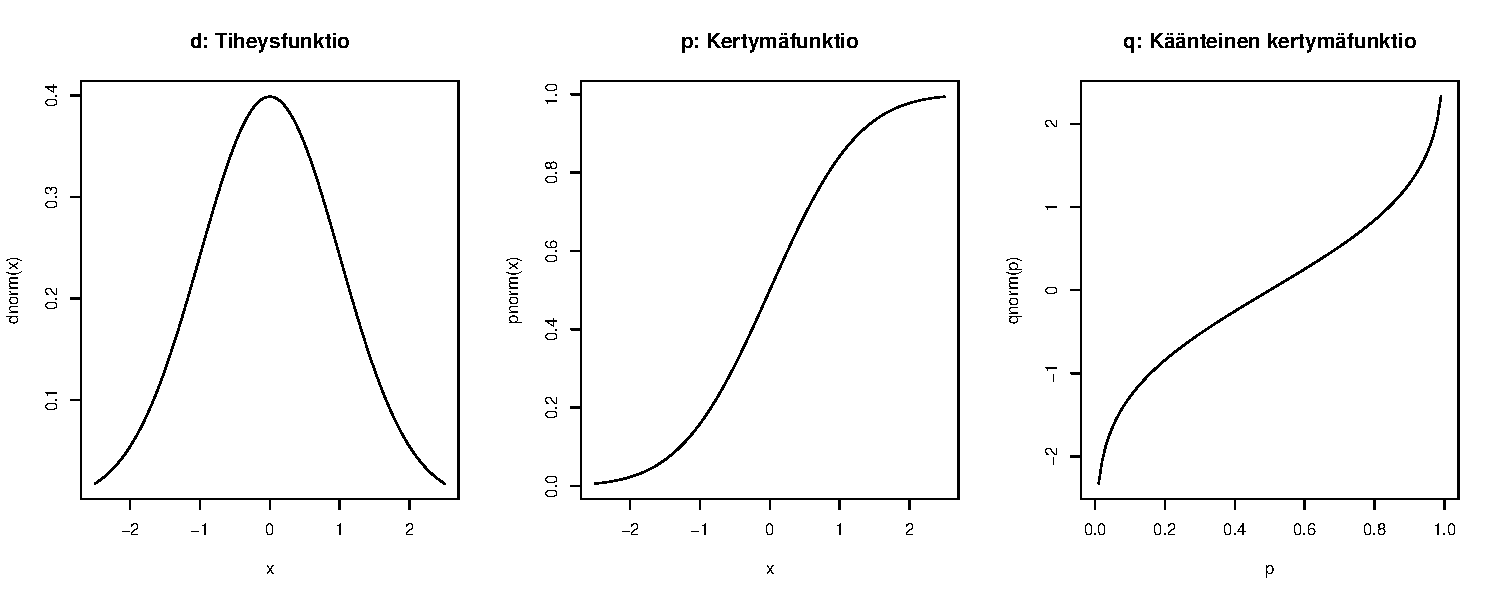
\includegraphics{R-ohjelmoinnin-perusteet_files/figure-latex/unnamed-chunk-97-1.pdf}

\hypertarget{esimerkki-normaalijakauma}{%
\section{Esimerkki: normaalijakauma}\label{esimerkki-normaalijakauma}}

Otetaan muutama käytännön esimerkki. Oletetaan, että suomalaisten miesten suolan saanti on normaalijakautunut odotusarvolla 10 grammaa päivässä ja keskihajonta on 4 grammaa päivässä (odotusarvo on totta, keskihajonta allekirjoittaneen hihasta). Piirretään ensin kuva jakaumasta välillä \([0, 20]\) grammaa päivässä. Jakauman muoto saadaan funktiolla \texttt{dnorm}, eli yllä olevan ohjeen mukaan d-alkuinen funktio antaa tiheysfunktion, ja norm-pääte viittaa normaalijakaumaan. Normaalijakauman funktiolle tulee kertoa jakauman odotusarvo (\texttt{mean}) ja keskihajonta (\texttt{sd}).

\begin{Shaded}
\begin{Highlighting}[]
\CommentTok{\# Sequential vector  of salt consumption}
\NormalTok{salt }\OtherTok{\textless{}{-}} \FunctionTok{seq}\NormalTok{(}\DecValTok{0}\NormalTok{, }\DecValTok{20}\NormalTok{, }\AttributeTok{by =} \FloatTok{0.1}\NormalTok{)}
\CommentTok{\# Density function}
\NormalTok{density }\OtherTok{\textless{}{-}} \FunctionTok{dnorm}\NormalTok{(salt, }\AttributeTok{mean =} \DecValTok{10}\NormalTok{, }\AttributeTok{sd =} \DecValTok{4}\NormalTok{)}
\CommentTok{\# Line plot}
\FunctionTok{plot}\NormalTok{(salt, density, }\AttributeTok{type =} \StringTok{"l"}\NormalTok{,}
     \AttributeTok{xlab =} \StringTok{"Suolan saanti"}\NormalTok{, }\AttributeTok{ylab =} \StringTok{"Tiheysfunktio"}\NormalTok{,}
     \AttributeTok{main =} \StringTok{"Suomalaisten miesten suolan saanti"}\NormalTok{)}
\end{Highlighting}
\end{Shaded}

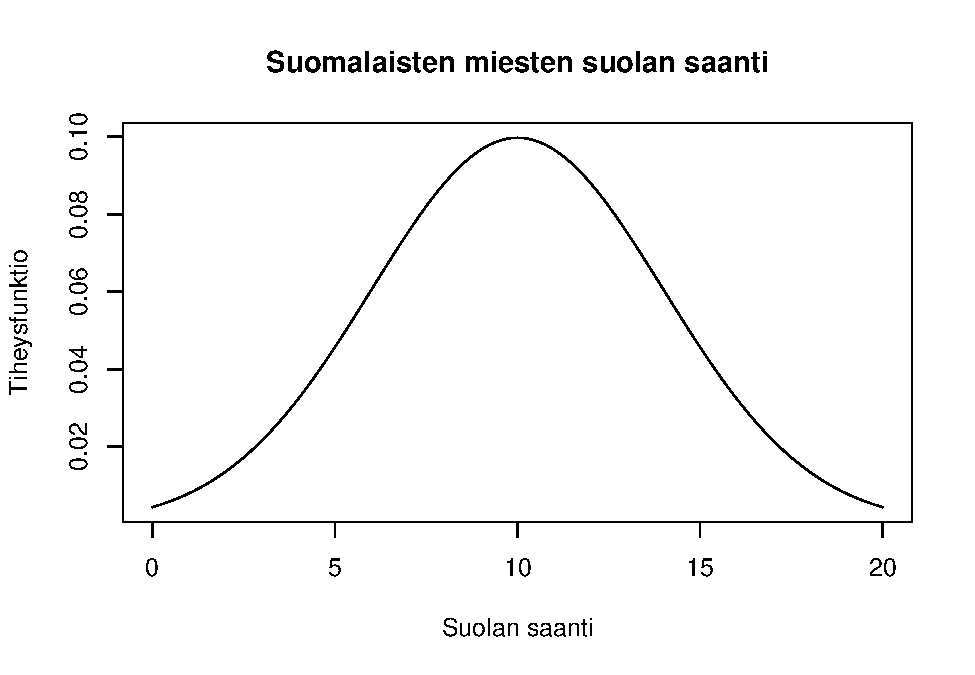
\includegraphics{R-ohjelmoinnin-perusteet_files/figure-latex/unnamed-chunk-98-1.pdf}

Aikuisten saantisuositus on enintään 5 grammaa suolaa päivässä. Kuinka moni suomalainen mies syö tämän jakauman mukaan sopivasti suolaa? Vastaus saadaan kertymäfunktiosta (\(P(X \leq 5)\)) \texttt{pnorm}-funktion avulla.

\begin{Shaded}
\begin{Highlighting}[]
\FunctionTok{pnorm}\NormalTok{(}\DecValTok{5}\NormalTok{, }\AttributeTok{mean =} \DecValTok{10}\NormalTok{, }\AttributeTok{sd =} \DecValTok{4}\NormalTok{)}
\end{Highlighting}
\end{Shaded}

\begin{verbatim}
## [1] 0.1056498
\end{verbatim}

Tämän jakauman mukaan vain noin 11 \% suomalaisista miehistä syö suolaa sopivasti!

Suomalaisten naiset syövät keskimäärin 7 grammaa suolaa päivässä. Kuinka moni mies syö tätä enemmän suolaa? \texttt{pnorm} antaa oletuksena arvon \(P(X \leq 7)\). Nyt halutaan kuitenkin tietää \(P(X > 7)\), joka saadaan asettamalla \texttt{lower.tail\ =\ FALSE}:

\begin{Shaded}
\begin{Highlighting}[]
\FunctionTok{pnorm}\NormalTok{(}\DecValTok{7}\NormalTok{, }\AttributeTok{mean =} \DecValTok{10}\NormalTok{, }\AttributeTok{sd =} \DecValTok{4}\NormalTok{, }\AttributeTok{lower.tail =} \ConstantTok{FALSE}\NormalTok{)}
\end{Highlighting}
\end{Shaded}

\begin{verbatim}
## [1] 0.7733726
\end{verbatim}

Noin 77 \% miehistä syö suolaa keskimääräistä naista enemmän.

Entä jos halutaan tietää, kuinka paljon suolaa eniten syövä 10 \% vähintään saa? Tähän voidaan vastata funktiolla \texttt{qnorm}, joka on jakauman käänteinen kertymäfunktio, eli funktion \texttt{pnorm} käänteisfunktio. Samoin kuin \texttt{pnorm}, \texttt{qnorm}-funktion oletus on, että todennäköisyydet lasketaan jakauman vasemmasta hännästä alkaen. Vastaus tähän kysymykseen selviää siis näillä kahdella tavalla:

\begin{Shaded}
\begin{Highlighting}[]
\FunctionTok{qnorm}\NormalTok{(}\FloatTok{0.1}\NormalTok{, }\AttributeTok{mean =} \DecValTok{10}\NormalTok{, }\AttributeTok{sd =} \DecValTok{4}\NormalTok{, }\AttributeTok{lower.tail =} \ConstantTok{FALSE}\NormalTok{)}
\end{Highlighting}
\end{Shaded}

\begin{verbatim}
## [1] 15.12621
\end{verbatim}

\begin{Shaded}
\begin{Highlighting}[]
\CommentTok{\# OR}
\FunctionTok{qnorm}\NormalTok{(}\FloatTok{0.9}\NormalTok{, }\AttributeTok{mean =} \DecValTok{10}\NormalTok{, }\AttributeTok{sd =} \DecValTok{4}\NormalTok{)}
\end{Highlighting}
\end{Shaded}

\begin{verbatim}
## [1] 15.12621
\end{verbatim}

Eli tämän jakauman mukaan eniten suolaa saava 10 \% miehistä syö yli kolminkertaisen määrän suolaa suositukseen verrattuna.

\hypertarget{muita-jakaumia}{%
\section{Muita jakaumia}\label{muita-jakaumia}}

Vastaavat funktiot löytyvät myös muille jakaumille, kuten:

\begin{itemize}
\tightlist
\item
  Khiin neliö: chisq
\item
  Eksponentiaalinen: exp
\item
  Studentin \(t\): t
\item
  Tasajakauma: unif
\end{itemize}

ja niin edelleen.

\hypertarget{plotting}{%
\chapter{Kuvaajien piirtäminen}\label{plotting}}

Tässä kappaleessa tutustutaan kuvaajien piirtämiseen.

R:n piirtokomennot voidaan jakaa kolmeen ryhmään:

\begin{itemize}
\tightlist
\item
  Korkean tason grafiikkatoiminnot piirtävät aina uuden kuvan
\item
  Alemman tason grafiikkatoiminnot lisäävät olemassa olevaan kuvaan uusia osia
\item
  Interaktiiviset grafiikkatoiminnot mahdollistavat vuorovaikutuksen kuvan kanssa. (Näiden käyttö on helpompaa opettaa videolla, joten niitä ei käsitellä tässä)
\end{itemize}

\hypertarget{korkean-tason-piirtofunktiot}{%
\section{Korkean tason piirtofunktiot}\label{korkean-tason-piirtofunktiot}}

\hypertarget{plot}{%
\subsection{plot}\label{plot}}

Korkean tason piirtofunktioista ylivoimaisesti yleisin on \texttt{plot}. \texttt{plot}-funktio on hyvin monipuolinen, mutta sen yleisin käyttötarkoitus on piirtää hajontakuvio (scatter plot) yhdestä tai kahdesta vektorista. Alla on hajontakuvio auton jarrutusmatkoista eri nopeuksilla:

\begin{Shaded}
\begin{Highlighting}[]
\CommentTok{\# Car speeds (km/h)}
\NormalTok{speed }\OtherTok{\textless{}{-}} \FunctionTok{seq}\NormalTok{(}\DecValTok{40}\NormalTok{, }\DecValTok{110}\NormalTok{, }\AttributeTok{by =} \DecValTok{10}\NormalTok{)}
\CommentTok{\# Stopping distances (m)}
\NormalTok{stop\_dist }\OtherTok{\textless{}{-}} \FunctionTok{c}\NormalTok{(}\DecValTok{26}\NormalTok{, }\DecValTok{35}\NormalTok{, }\DecValTok{45}\NormalTok{, }\DecValTok{56}\NormalTok{, }\DecValTok{69}\NormalTok{, }\DecValTok{83}\NormalTok{, }\DecValTok{98}\NormalTok{, }\DecValTok{113}\NormalTok{)}

\FunctionTok{plot}\NormalTok{(}\AttributeTok{x =}\NormalTok{ speed, }\AttributeTok{y =}\NormalTok{ stop\_dist)}
\end{Highlighting}
\end{Shaded}

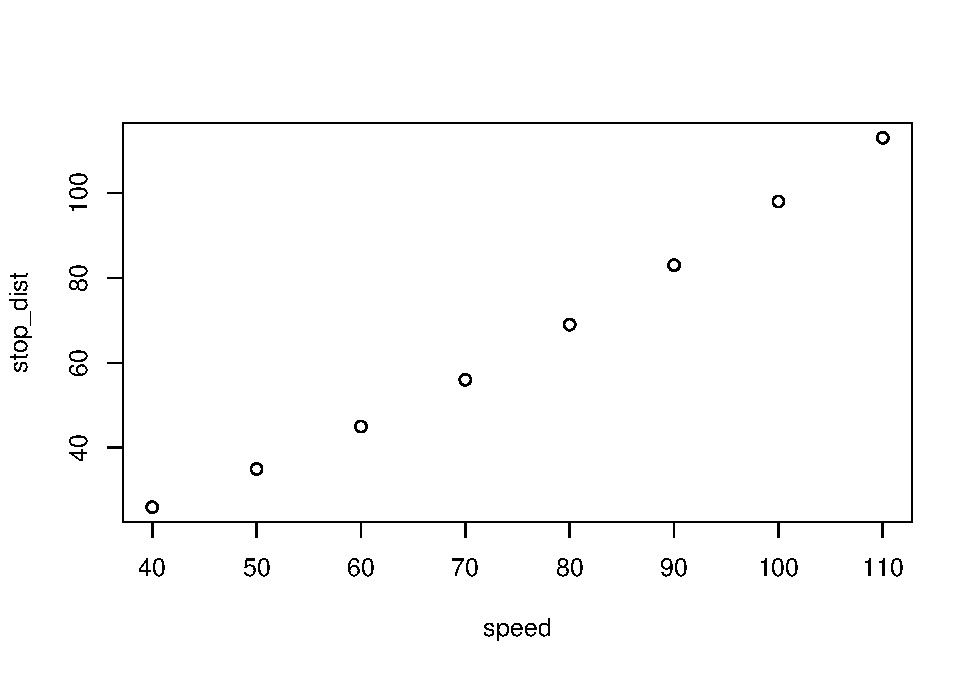
\includegraphics{R-ohjelmoinnin-perusteet_files/figure-latex/unnamed-chunk-102-1.pdf}

\texttt{plot}-funktiolle annetaan siis kaksi yhtä pitkää vektoria, joissa ovat pisteiden \(x\)- ja \(y\)-koordinaatit. Halutessaan kuvalle voi antaa otsikon (title) ja nimetä uudestaan kuvan akselit (axis labels). Tämä onkin usein hyvä idea, sillä R:n muuttujien nimissä ei saa olla välilyöntejä tai erikoismerkkejä, mutta usein näiden käyttö akselien nimissä on hyvin informatiivista.

\begin{Shaded}
\begin{Highlighting}[]
\FunctionTok{plot}\NormalTok{(}\AttributeTok{x =}\NormalTok{ speed, }\AttributeTok{y =}\NormalTok{ stop\_dist,}
     \AttributeTok{main =} \StringTok{"Auton pysähtymismatka eri nopeuksilla"}\NormalTok{,}
     \AttributeTok{xlab =} \StringTok{"Auton nopeus (km / h)"}\NormalTok{, }\AttributeTok{ylab =} \StringTok{"Pysähtymismatka (m)"}\NormalTok{)}
\end{Highlighting}
\end{Shaded}

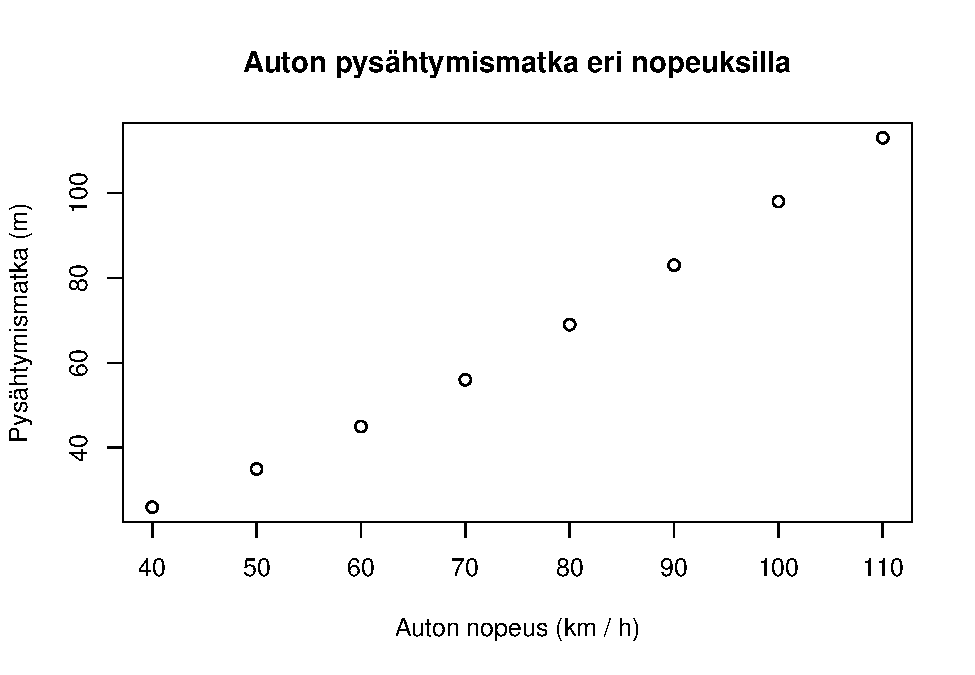
\includegraphics{R-ohjelmoinnin-perusteet_files/figure-latex/unnamed-chunk-103-1.pdf}

\texttt{plot}-funktiolle voi antaa muitakin argumentteja, jotka säätävät mm. pisteiden väriä, kokoa ja muotoa, akselien rajoja jne. Yleisiä kuvaajien parametreja voi säätää funktiolla `\texttt{par} (graphical parameters).

\hypertarget{muut-korkean-tason-funktiot}{%
\subsection{Muut korkean tason funktiot}\label{muut-korkean-tason-funktiot}}

Tässä on esimerkkejä muutamista muista yleisistä korkean tason funktioista:

\texttt{hist} piirtää histogrammeja. Histogrammit kuvaavat jatkuvan muuttujan jakaumaa.

\begin{Shaded}
\begin{Highlighting}[]
\CommentTok{\# A vector of 1000 observations from a normal distribution of heights of Finnish women}
\NormalTok{heights }\OtherTok{\textless{}{-}} \FunctionTok{rnorm}\NormalTok{(}\AttributeTok{n =} \DecValTok{1000}\NormalTok{, }\AttributeTok{mean =} \DecValTok{168}\NormalTok{, }\AttributeTok{sd =} \FloatTok{5.4}\NormalTok{)}
\FunctionTok{hist}\NormalTok{(heights, }\AttributeTok{breaks =} \DecValTok{20}\NormalTok{, }
     \AttributeTok{main =} \StringTok{"Suomalaisten naisten pituuksien jakauma"}\NormalTok{,}
     \AttributeTok{xlab =} \StringTok{"Pituus (cm)"}\NormalTok{, }\AttributeTok{ylab =} \StringTok{"Frekvenssi"}\NormalTok{)}
\end{Highlighting}
\end{Shaded}

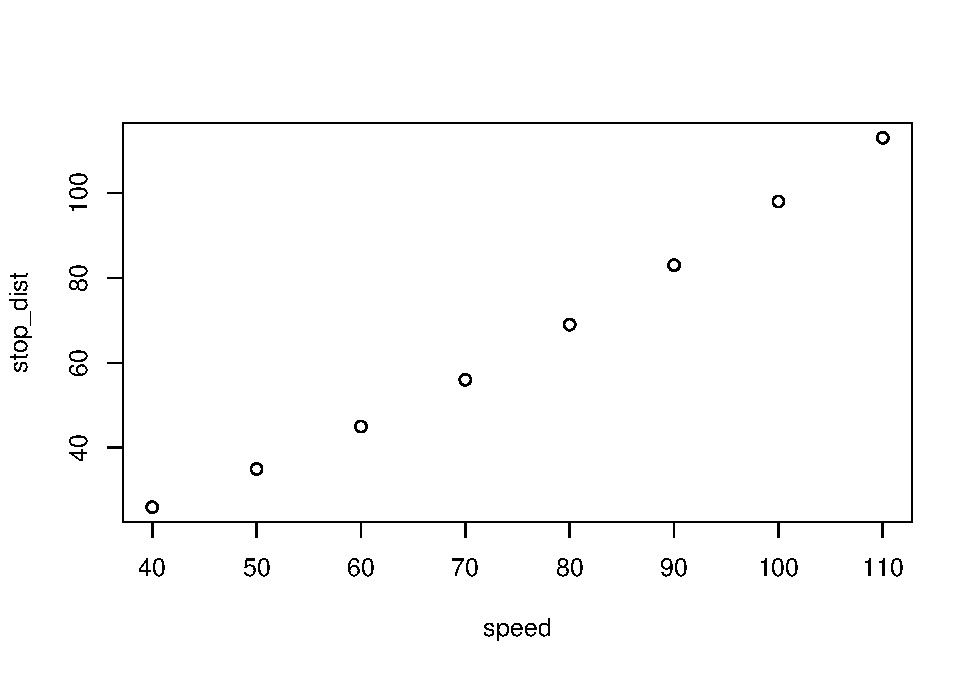
\includegraphics{R-ohjelmoinnin-perusteet_files/figure-latex/unnamed-chunk-104-1.pdf}

Toinen tapa kuvata jatkuvan muuttujan jakaumaa on viiksilaatikko (joskus myös laatikko-viikset -kuvaaja), joita piirretään \texttt{boxplot}-funktiolla:

\begin{Shaded}
\begin{Highlighting}[]
\FunctionTok{boxplot}\NormalTok{(heights, }\AttributeTok{breaks =} \DecValTok{20}\NormalTok{, }
     \AttributeTok{main =} \StringTok{"Suomalaisten naisten pituuksien jakauma"}\NormalTok{,}
     \AttributeTok{ylab =} \StringTok{"Pituus (cm)"}\NormalTok{)}
\end{Highlighting}
\end{Shaded}

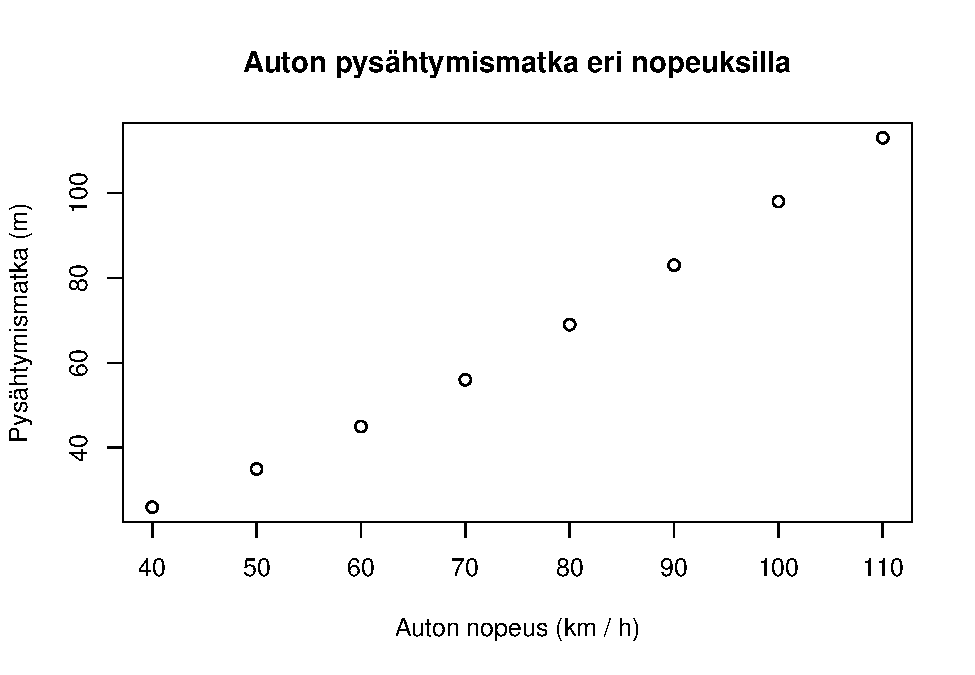
\includegraphics{R-ohjelmoinnin-perusteet_files/figure-latex/unnamed-chunk-105-1.pdf}

Vastaavasti diskreetin muuttujan jakaumaa voi kuvata pylväsdiagrammilla käyttäen \texttt{barplot}-funktiota. Alla on esimerkki opiskelijoiden kotipaikkakuntien jakaumasta. Tässä tulee myös tutuksi uusi vektorien ominaisuus: nimeäminen. Nimettyjen vektorien (named vectors) alkioilla on järjestyslukujen lisäksi nimet. Nimet annetaan olla olevaan tyyliin \texttt{nimi\ =\ alkio}. Nimetyt vektori käyttäytyvät aivan kuin tavalliset vektorit, mutta niitä voi indeksoida myös nimien avulla, ja jotkut funktiot, kuten barplot, käyttävät hyödyksi alkioiden nimiä. Nimettyjen vektorien käyttö ei ole kurssin ydinasioita, mutta on joskus hyvin kätevä temppu osata.

\begin{Shaded}
\begin{Highlighting}[]
\NormalTok{origin }\OtherTok{\textless{}{-}} \FunctionTok{c}\NormalTok{(}\StringTok{"Pohjois{-}Savo"} \OtherTok{=} \DecValTok{15}\NormalTok{, }\StringTok{"Pk{-}seutu"} \OtherTok{=} \DecValTok{10}\NormalTok{, }\StringTok{"Turku"} \OtherTok{=} \DecValTok{3}\NormalTok{,}
            \StringTok{"Pohjois{-}Suomi"} \OtherTok{=} \DecValTok{8}\NormalTok{)}
\NormalTok{origin}
\end{Highlighting}
\end{Shaded}

\begin{verbatim}
##  Pohjois-Savo      Pk-seutu         Turku Pohjois-Suomi 
##            15            10             3             8
\end{verbatim}

\begin{Shaded}
\begin{Highlighting}[]
\NormalTok{origin[}\StringTok{"Turku"}\NormalTok{]}
\end{Highlighting}
\end{Shaded}

\begin{verbatim}
## Turku 
##     3
\end{verbatim}

\begin{Shaded}
\begin{Highlighting}[]
\FunctionTok{barplot}\NormalTok{(origin, }
        \AttributeTok{main =} \StringTok{"Opiskelijoiden kotipaikkakunta"}\NormalTok{,}
        \AttributeTok{ylab =} \StringTok{"Opiskelijoiden lukumäärä"}\NormalTok{)}
\end{Highlighting}
\end{Shaded}

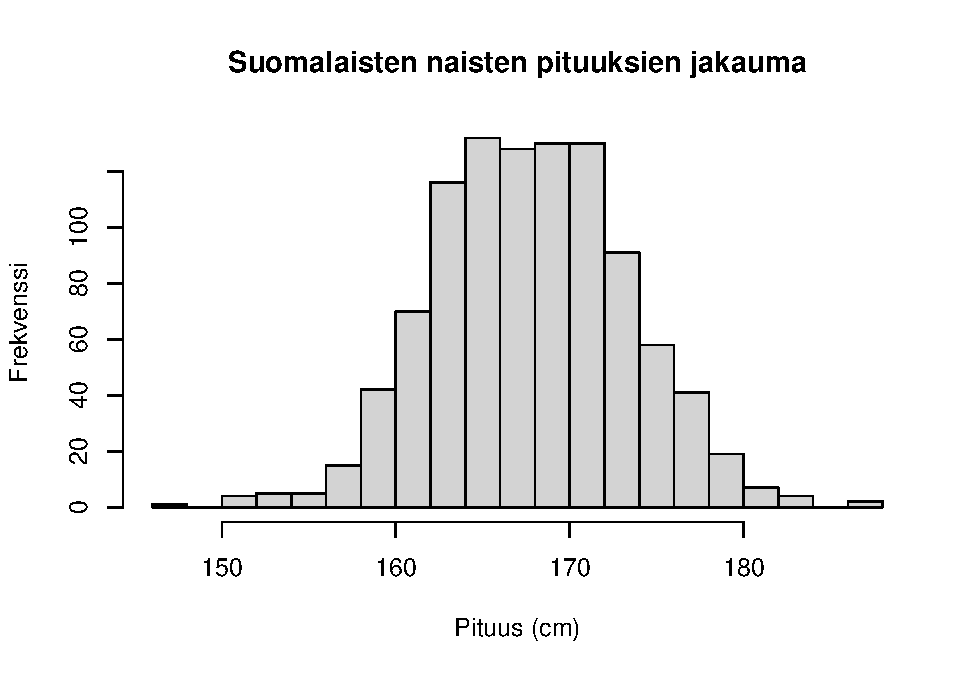
\includegraphics{R-ohjelmoinnin-perusteet_files/figure-latex/unnamed-chunk-106-1.pdf}

\hypertarget{alemman-tason-grafiikkatoiminnot}{%
\section{Alemman tason grafiikkatoiminnot}\label{alemman-tason-grafiikkatoiminnot}}

Alemman tason grafiikkatoiminnoilla voi lisätä olemassa olevaan kuvaan lisää osia, kuten tekstiä, pisteitä tai selitteen (legend).

Otetaan esimerkiksi alussa nähty kuvaaja autojen pysähtymismatkoista ja lisätään siihen uusia osia. Tässä vielä alkuperäinen kuva:

\begin{Shaded}
\begin{Highlighting}[]
\FunctionTok{plot}\NormalTok{(}\AttributeTok{x =}\NormalTok{ speed, }\AttributeTok{y =}\NormalTok{ stop\_dist,}
     \AttributeTok{main =} \StringTok{"Auton pysähtymismatka eri nopeuksilla"}\NormalTok{,}
     \AttributeTok{xlab =} \StringTok{"Auton nopeus (km / h)"}\NormalTok{, }\AttributeTok{ylab =} \StringTok{"Pysähtymismatka (m)"}\NormalTok{)}
\end{Highlighting}
\end{Shaded}

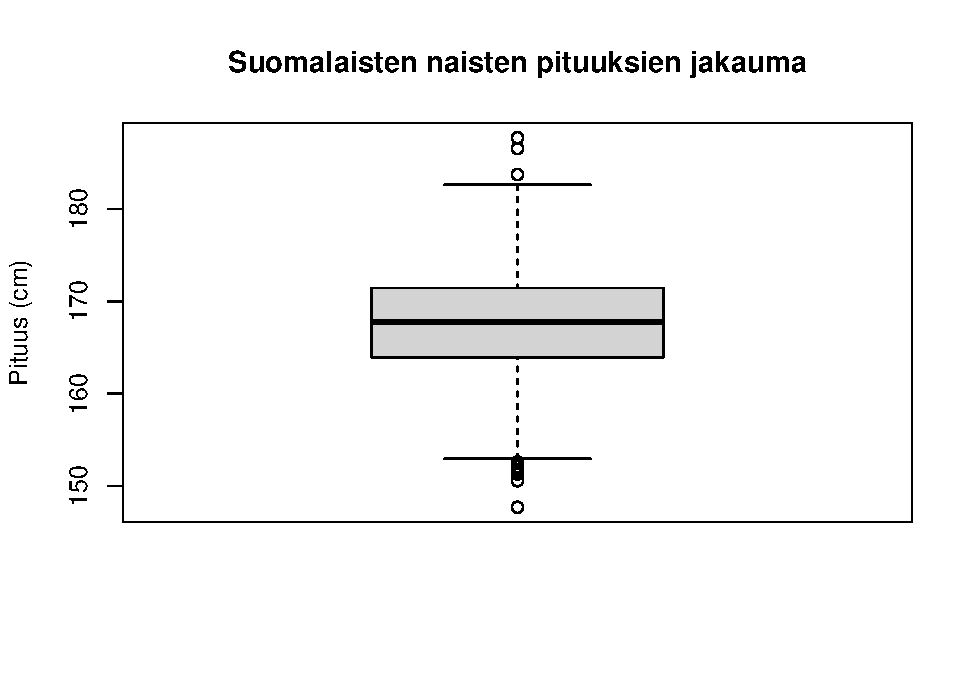
\includegraphics{R-ohjelmoinnin-perusteet_files/figure-latex/unnamed-chunk-107-1.pdf}

Lisätään kuvaajan jarrutusmatkat liukkaalla kelillä. Uusia pisteitä voi piirtää \texttt{points}-funktiolla, jolle annetaan x- ja y-koordinaatit vektoreina ihan kuin \texttt{plot}-funktiollekin.

\begin{Shaded}
\begin{Highlighting}[]
\NormalTok{stop\_dist\_wet }\OtherTok{\textless{}{-}} \FunctionTok{c}\NormalTok{(}\DecValTok{30}\NormalTok{, }\DecValTok{41}\NormalTok{, }\DecValTok{54}\NormalTok{, }\DecValTok{69}\NormalTok{, }\DecValTok{85}\NormalTok{, }\DecValTok{103}\NormalTok{, }\DecValTok{122}\NormalTok{, }\DecValTok{143}\NormalTok{)}
\FunctionTok{plot}\NormalTok{(}\AttributeTok{x =}\NormalTok{ speed, }\AttributeTok{y =}\NormalTok{ stop\_dist,}
     \AttributeTok{main =} \StringTok{"Auton pysähtymismatka eri nopeuksilla"}\NormalTok{,}
     \AttributeTok{xlab =} \StringTok{"Auton nopeus (km / h)"}\NormalTok{, }\AttributeTok{ylab =} \StringTok{"Pysähtymismatka (m)"}\NormalTok{)}
\FunctionTok{points}\NormalTok{(}\AttributeTok{x =}\NormalTok{ speed, }\AttributeTok{y =}\NormalTok{ stop\_dist\_wet)}
\end{Highlighting}
\end{Shaded}

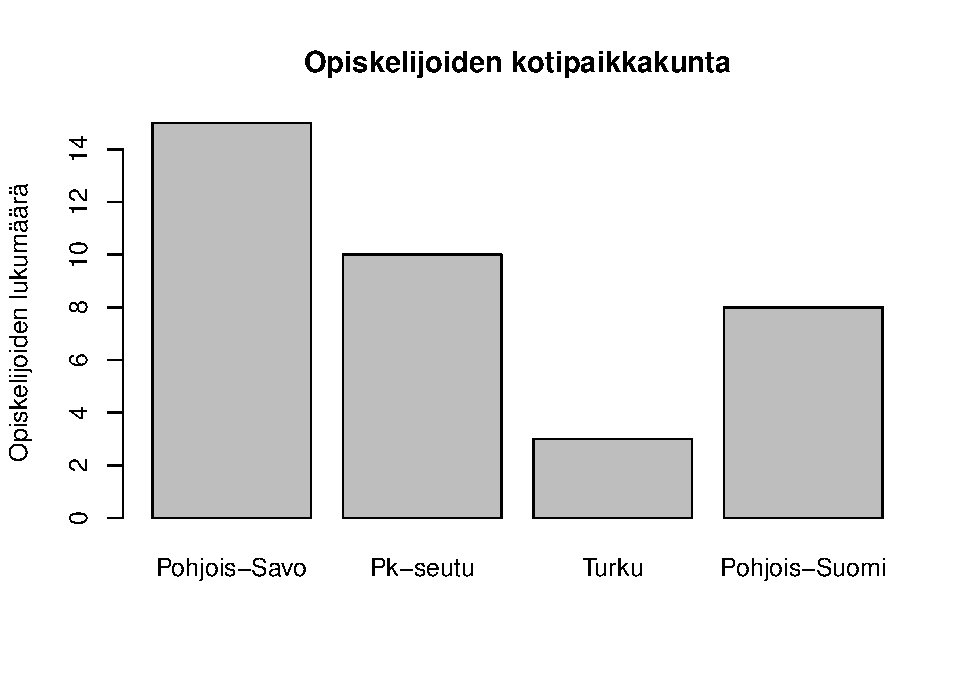
\includegraphics{R-ohjelmoinnin-perusteet_files/figure-latex/unnamed-chunk-108-1.pdf}

Ylläolevassa kuvaajassa on kaksi ongelmaa: ylimmät pisteet eivät näy, koska kuvaajan y-akseli loppuu kesken. \(y\)-akseli on piirretty alkuperäisten jarrutusmatkojen pohjalta, ja koska liukkaalla kelillä jarrutus kestää pidempään, uudet pisteet eivät mahdu kuvaajaan. Toinen ongelma on se, että pisteitä ei voi erottaa toisistaan.

Ensimmäinen ongelma ratkeaa säätämällä käsin \(y\)-akselin rajat. Tämä tapahtuu argumentilla \texttt{ylim}, jolle annetaan vektorissa ylä- ja alaraja (vastaavasti \texttt{xlim} säätää \(x\)-akselin rajat).

Lisäksi piirretään selvyyden vuoksi pisteet eri värisinä ja eri kuvioilla. Argumentti \texttt{col} säätää pisteiden värin ja \texttt{pch} pisteiden muodon. Eri väri- ja muotovaihtoehdot löytyvät googlaamalla.

\begin{Shaded}
\begin{Highlighting}[]
\FunctionTok{plot}\NormalTok{(}\AttributeTok{x =}\NormalTok{ speed, }\AttributeTok{y =}\NormalTok{ stop\_dist,}
     \AttributeTok{col =} \StringTok{"darkblue"}\NormalTok{, }\AttributeTok{pch =} \DecValTok{20}\NormalTok{,}
     \AttributeTok{ylim =} \FunctionTok{c}\NormalTok{(}\DecValTok{20}\NormalTok{, }\DecValTok{150}\NormalTok{),}
     \AttributeTok{main =} \StringTok{"Auton pysähtymismatka eri nopeuksilla"}\NormalTok{,}
     \AttributeTok{xlab =} \StringTok{"Auton nopeus (km / h)"}\NormalTok{, }\AttributeTok{ylab =} \StringTok{"Pysähtymismatka (m)"}\NormalTok{)}
\FunctionTok{points}\NormalTok{(}\AttributeTok{x =}\NormalTok{ speed, }\AttributeTok{y =}\NormalTok{ stop\_dist\_wet, }\AttributeTok{pch =} \DecValTok{15}\NormalTok{, }\AttributeTok{col =} \StringTok{"darkred"}\NormalTok{)}
\end{Highlighting}
\end{Shaded}

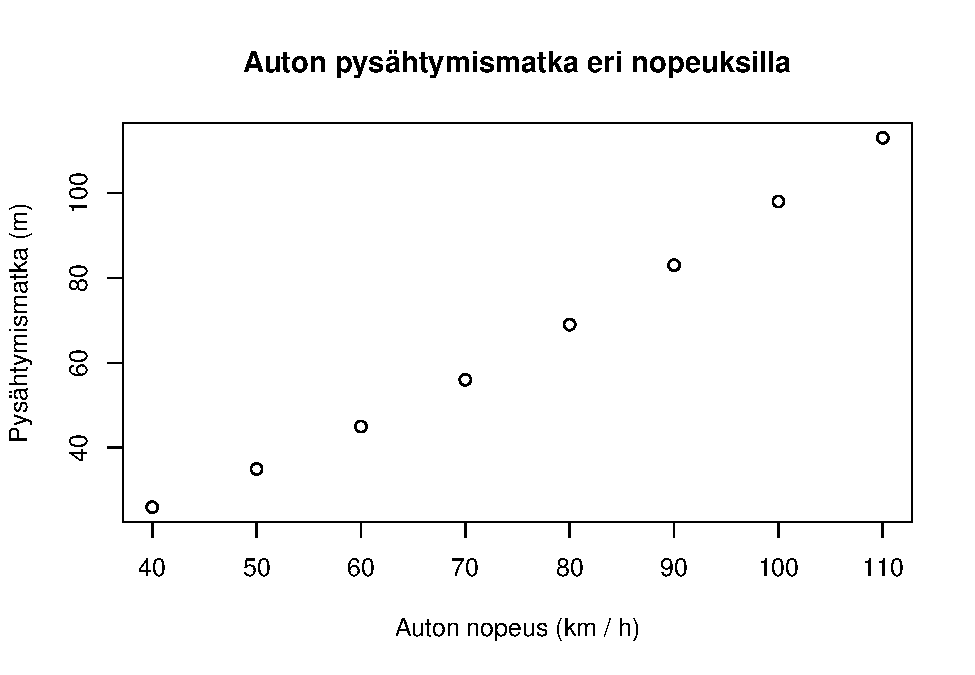
\includegraphics{R-ohjelmoinnin-perusteet_files/figure-latex/unnamed-chunk-109-1.pdf}

Nyt kuvaaja alkaa jo näyttää paremmalta, mutta kuvaajasta ei vielä voi päätellä, mitä eri väriset pisteet tarkoittavat. Lisätään siis kuvaajaan selite \texttt{legend}-komennolla. Selitteelle määritetään paikka kuvaajassa \texttt{x} ja \texttt{y} argumenteilla (vasemman yläkulman koordinaatit). Sen jälkeen annetaan selitetekstit (\texttt{legend}), sekä selitteen muodot ja värit (\texttt{pch} ja \texttt{col}, kuten aiemmin). HUOM! Selitteen symbolit ja värit on itse osattava laittaa oikeaan järjestykseen. Selitteen tekstit annetaan järjestyksessä ylhäältä alas, ja piirtomerkit tulee antaa samassa järjestyksessä.

\begin{Shaded}
\begin{Highlighting}[]
\FunctionTok{plot}\NormalTok{(}\AttributeTok{x =}\NormalTok{ speed, }\AttributeTok{y =}\NormalTok{ stop\_dist,}
     \AttributeTok{col =} \StringTok{"darkblue"}\NormalTok{, }\AttributeTok{pch =} \DecValTok{20}\NormalTok{,}
     \AttributeTok{ylim =} \FunctionTok{c}\NormalTok{(}\DecValTok{20}\NormalTok{, }\DecValTok{150}\NormalTok{),}
     \AttributeTok{main =} \StringTok{"Auton pysähtymismatka eri nopeuksilla"}\NormalTok{,}
     \AttributeTok{xlab =} \StringTok{"Auton nopeus (km / h)"}\NormalTok{, }\AttributeTok{ylab =} \StringTok{"Pysähtymismatka (m)"}\NormalTok{)}

\FunctionTok{points}\NormalTok{(}\AttributeTok{x =}\NormalTok{ speed, }\AttributeTok{y =}\NormalTok{ stop\_dist\_wet, }\AttributeTok{pch =} \DecValTok{15}\NormalTok{, }\AttributeTok{col =} \StringTok{"darkred"}\NormalTok{)}

\FunctionTok{legend}\NormalTok{(}\AttributeTok{x =} \DecValTok{40}\NormalTok{, }\AttributeTok{y =} \DecValTok{150}\NormalTok{,}
       \AttributeTok{legend =} \FunctionTok{c}\NormalTok{(}\StringTok{"Märkä keli"}\NormalTok{, }\StringTok{"Kuiva keli"}\NormalTok{),}
       \AttributeTok{pch =} \FunctionTok{c}\NormalTok{(}\DecValTok{15}\NormalTok{, }\DecValTok{20}\NormalTok{), }\AttributeTok{col =} \FunctionTok{c}\NormalTok{(}\StringTok{"darkred"}\NormalTok{, }\StringTok{"darkblue"}\NormalTok{))}
\end{Highlighting}
\end{Shaded}

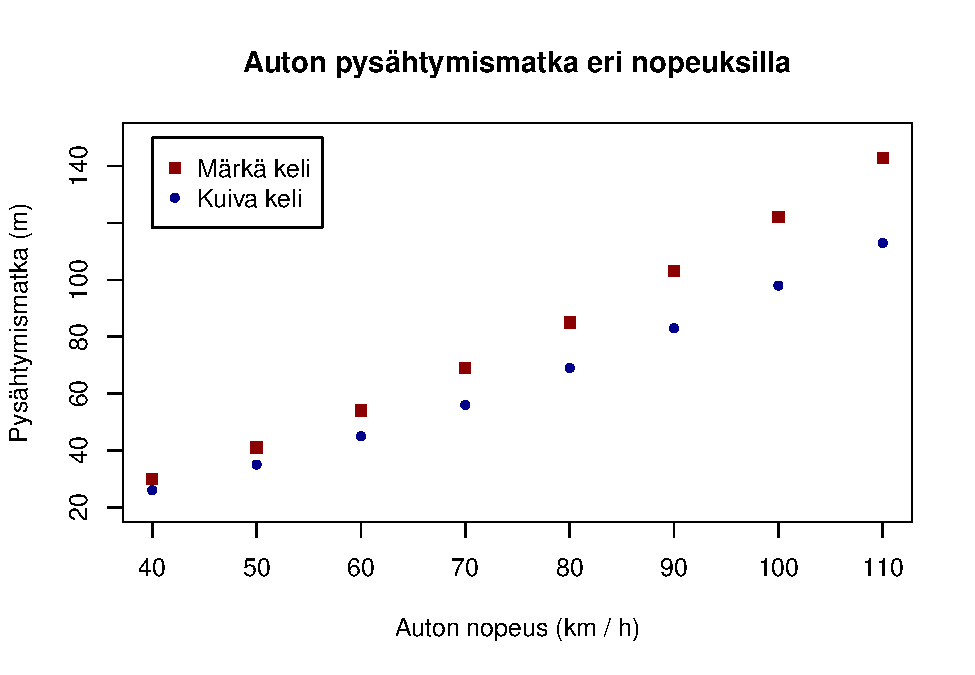
\includegraphics{R-ohjelmoinnin-perusteet_files/figure-latex/unnamed-chunk-110-1.pdf}

Tuunataan kuvaajaa vielä hiukan, ja lisätään siihen käyrä kuvaamaan jarrutusmatkan ennustetta \texttt{lines}-funktiolla.

Alla olevassa koodissa lasketaan ensin \texttt{lm}-funktion avulla sopivat parametrit käyrälle. Lineaarisia malleja käsitellään vasta kappaleessa \protect\hyperlink{linear_models}{lineaariset mallit}, joten tässä vaiheessa niistä ei tarvitse vielä ymmärtää muuta kuin se, että \texttt{lm}-funktio sovittaa lineaarisen mallin (tässä tapauksessa muotoa \(\text{matka} = a + b \cdot \text{nopeus} + c \cdot \text{nopeus}^2)\), jonka perusteella voidaan ennustaa pysähtymismatkaa myös muille kuin mitatuille nopeuksille.

\begin{Shaded}
\begin{Highlighting}[]
\CommentTok{\# Create vecotr of squared speeds to fit second order polynomial}
\NormalTok{speed\_squared }\OtherTok{\textless{}{-}}\NormalTok{ speed}\SpecialCharTok{\^{}}\DecValTok{2}

\CommentTok{\# Model for dry weather}
\NormalTok{model\_dry }\OtherTok{\textless{}{-}} \FunctionTok{lm}\NormalTok{(stop\_dist }\SpecialCharTok{\textasciitilde{}}\NormalTok{ speed }\SpecialCharTok{+}\NormalTok{ speed\_squared)}
\NormalTok{prediction\_dry }\OtherTok{\textless{}{-}}\NormalTok{ model\_dry}\SpecialCharTok{$}\NormalTok{fitted.values}

\CommentTok{\# Model for rainy weather}
\NormalTok{model\_wet }\OtherTok{\textless{}{-}} \FunctionTok{lm}\NormalTok{(stop\_dist\_wet }\SpecialCharTok{\textasciitilde{}}\NormalTok{ speed }\SpecialCharTok{+}\NormalTok{ speed\_squared)}
\NormalTok{prediction\_wet }\OtherTok{\textless{}{-}}\NormalTok{ model\_wet}\SpecialCharTok{$}\NormalTok{fitted.values}
\end{Highlighting}
\end{Shaded}

\texttt{lines} tarvitsee \texttt{x} ja \texttt{y} argumentit kuten \texttt{points}, mutta piirtää viivan, ei pisteitä. Käytetään äsken laskettuja mallien antamia \texttt{prediction}-vektoreita y-koordinaatteina. Tehdään viivoista katkoviivoja argumentilla \texttt{lty\ =\ "dashed"} (lty = line type).

\begin{Shaded}
\begin{Highlighting}[]
\FunctionTok{plot}\NormalTok{(}\AttributeTok{x =}\NormalTok{ speed, }\AttributeTok{y =}\NormalTok{ stop\_dist,}
     \AttributeTok{col =} \StringTok{"darkblue"}\NormalTok{, }\AttributeTok{pch =} \DecValTok{20}\NormalTok{,}
     \AttributeTok{ylim =} \FunctionTok{c}\NormalTok{(}\DecValTok{20}\NormalTok{, }\DecValTok{150}\NormalTok{),}
     \AttributeTok{main =} \StringTok{"Auton pysähtymismatka eri nopeuksilla"}\NormalTok{,}
     \AttributeTok{xlab =} \StringTok{"Auton nopeus (km / h)"}\NormalTok{, }\AttributeTok{ylab =} \StringTok{"Pysähtymismatka (m)"}\NormalTok{)}

\FunctionTok{points}\NormalTok{(}\AttributeTok{x =}\NormalTok{ speed, }\AttributeTok{y =}\NormalTok{ stop\_dist\_wet, }\AttributeTok{pch =} \DecValTok{15}\NormalTok{, }\AttributeTok{col =} \StringTok{"darkred"}\NormalTok{)}

\FunctionTok{legend}\NormalTok{(}\AttributeTok{x =} \DecValTok{40}\NormalTok{, }\AttributeTok{y =} \DecValTok{150}\NormalTok{,}
       \AttributeTok{legend =} \FunctionTok{c}\NormalTok{(}\StringTok{"Märkä keli"}\NormalTok{, }\StringTok{"Kuiva keli"}\NormalTok{),}
       \AttributeTok{pch =} \FunctionTok{c}\NormalTok{(}\DecValTok{15}\NormalTok{, }\DecValTok{20}\NormalTok{), }\AttributeTok{col =} \FunctionTok{c}\NormalTok{(}\StringTok{"darkred"}\NormalTok{, }\StringTok{"darkblue"}\NormalTok{))}

\FunctionTok{lines}\NormalTok{(speed, prediction\_dry, }\AttributeTok{lty =} \StringTok{"dashed"}\NormalTok{)}
\FunctionTok{lines}\NormalTok{(speed, prediction\_wet, }\AttributeTok{lty =} \StringTok{"dashed"}\NormalTok{)}
\end{Highlighting}
\end{Shaded}

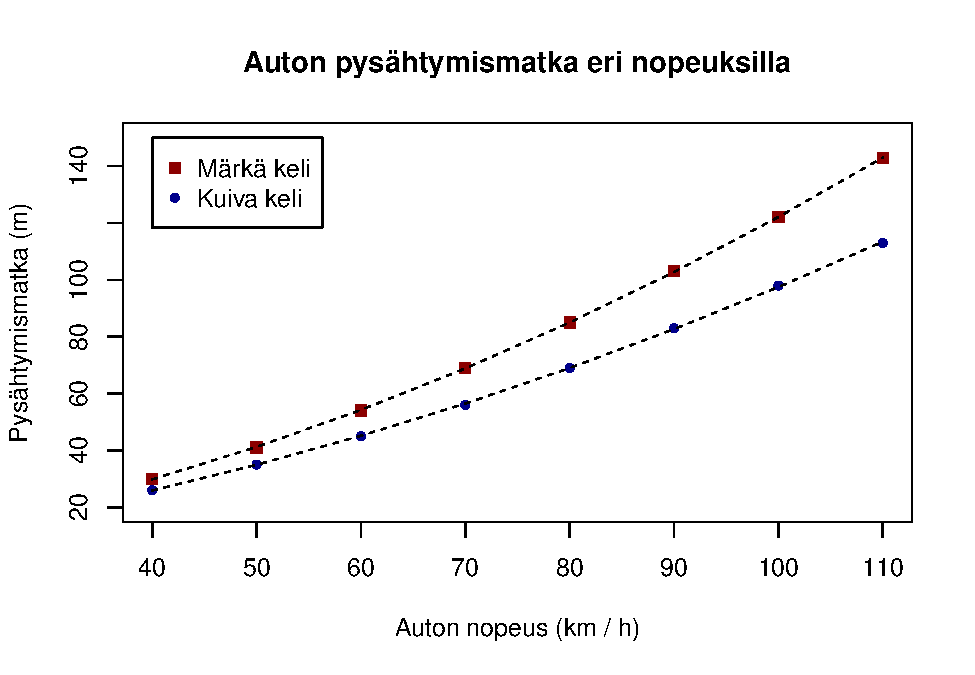
\includegraphics{R-ohjelmoinnin-perusteet_files/figure-latex/unnamed-chunk-112-1.pdf}

Seuraavaksi voidaan värittää käyrät samoilla väreillä kuin pisteet, ja lisätä niille omat selitteet. Tässä vaiheessa selitteen tekemisestä tulee jo melko monimutkaista, sillä selitteessä on mukana pisteitä ja käyriä. Tästä syystä selitteen argumentteihin pitää laittaa puuttuvia arvoja \texttt{pch} ja \texttt{lty}-argumenteille, koska selitteen ensimmäiset rivit eivät viittaa mihinkään käyrään, vaan pelkästään pisteisiin ja vastaavasti kaksi alinta riviä viittaavat vain käyriin.

\begin{Shaded}
\begin{Highlighting}[]
\FunctionTok{plot}\NormalTok{(}\AttributeTok{x =}\NormalTok{ speed, }\AttributeTok{y =}\NormalTok{ stop\_dist,}
     \AttributeTok{col =} \StringTok{"darkblue"}\NormalTok{, }\AttributeTok{pch =} \DecValTok{20}\NormalTok{,}
     \AttributeTok{ylim =} \FunctionTok{c}\NormalTok{(}\DecValTok{20}\NormalTok{, }\DecValTok{150}\NormalTok{),}
     \AttributeTok{main =} \StringTok{"Auton pysähtymismatka eri nopeuksilla"}\NormalTok{,}
     \AttributeTok{xlab =} \StringTok{"Auton nopeus (km / h)"}\NormalTok{, }\AttributeTok{ylab =} \StringTok{"Pysähtymismatka (m)"}\NormalTok{)}

\FunctionTok{points}\NormalTok{(}\AttributeTok{x =}\NormalTok{ speed, }\AttributeTok{y =}\NormalTok{ stop\_dist\_wet, }\AttributeTok{pch =} \DecValTok{15}\NormalTok{, }\AttributeTok{col =} \StringTok{"darkred"}\NormalTok{)}

\FunctionTok{legend}\NormalTok{(}\AttributeTok{x =} \DecValTok{40}\NormalTok{, }\AttributeTok{y =} \DecValTok{150}\NormalTok{,}
       \AttributeTok{legend =} \FunctionTok{c}\NormalTok{(}\StringTok{"Märkä keli"}\NormalTok{, }\StringTok{"Kuiva keli"}\NormalTok{,}
                  \StringTok{"Ennuste märälle kelille"}\NormalTok{,}
                  \StringTok{"Ennuste kuivalle kelille"}\NormalTok{),}
       \AttributeTok{pch =} \FunctionTok{c}\NormalTok{(}\DecValTok{15}\NormalTok{, }\DecValTok{20}\NormalTok{, }\ConstantTok{NA}\NormalTok{, }\ConstantTok{NA}\NormalTok{),}
       \AttributeTok{lty =} \FunctionTok{c}\NormalTok{(}\ConstantTok{NA}\NormalTok{, }\ConstantTok{NA}\NormalTok{, }\StringTok{"dashed"}\NormalTok{, }\StringTok{"dashed"}\NormalTok{),}
       \AttributeTok{col =} \FunctionTok{c}\NormalTok{(}\StringTok{"darkred"}\NormalTok{, }\StringTok{"darkblue"}\NormalTok{, }\StringTok{"darkred"}\NormalTok{, }\StringTok{"darkblue"}\NormalTok{))}

\FunctionTok{lines}\NormalTok{(speed, prediction\_dry, }\AttributeTok{lty =} \StringTok{"dashed"}\NormalTok{, }\AttributeTok{col =} \StringTok{"darkblue"}\NormalTok{)}
\FunctionTok{lines}\NormalTok{(speed, prediction\_wet, }\AttributeTok{lty =} \StringTok{"dashed"}\NormalTok{, }\AttributeTok{col =} \StringTok{"darkred"}\NormalTok{)}
\end{Highlighting}
\end{Shaded}

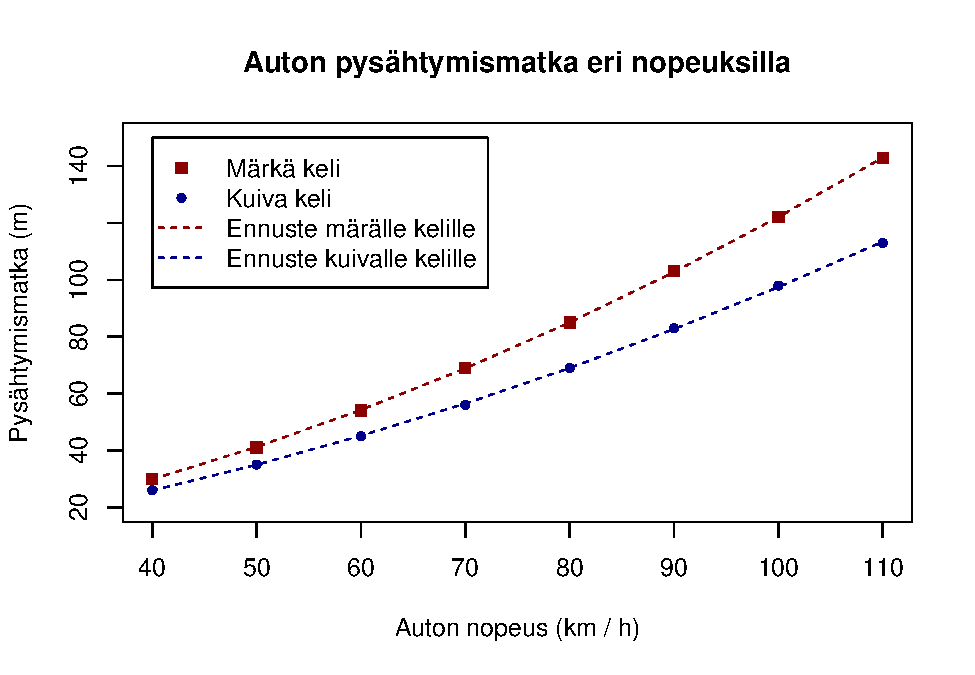
\includegraphics{R-ohjelmoinnin-perusteet_files/figure-latex/unnamed-chunk-113-1.pdf}

Kuvaajamme on melkein valmis iltapäivälehteen muistuttamaan liukkaiden kelien vaaroista, mutta jotta siitä tulisi oikein säväyttävä, siinä pitää toki olla tekstiä! Lisätään siis vielä pieni tekstin pätkä, joka korostaa eroa liukkaan ja kuivan kelin välillä. Tekstiä voi lisätä \texttt{text}-funktiolla, jolle annetaan tuttuun tapaan \texttt{x} ja \texttt{y}-argumentit, joilla määritetään tekstin paikka ja \texttt{labels} määrittää itse tekstin (kaikki argumentit voivat olla myös pidempiä vektoreita, jolloin tulee useampi teksti eri paikkoihin). Lisäksi parametrillä \texttt{adj} (adjust) voi hienosäätää tekstin paikkaa. \texttt{adj} on vektori, jossa on hienosäätöarvot \(x\)- ja \(y\)-suunnissa.

\begin{Shaded}
\begin{Highlighting}[]
\FunctionTok{plot}\NormalTok{(}\AttributeTok{x =}\NormalTok{ speed, }\AttributeTok{y =}\NormalTok{ stop\_dist,}
     \AttributeTok{col =} \StringTok{"darkblue"}\NormalTok{, }\AttributeTok{pch =} \DecValTok{20}\NormalTok{,}
     \AttributeTok{ylim =} \FunctionTok{c}\NormalTok{(}\DecValTok{20}\NormalTok{, }\DecValTok{150}\NormalTok{),}
     \AttributeTok{main =} \StringTok{"Auton pysähtymismatka eri nopeuksilla"}\NormalTok{,}
     \AttributeTok{xlab =} \StringTok{"Auton nopeus (km / h)"}\NormalTok{, }\AttributeTok{ylab =} \StringTok{"Pysähtymismatka (m)"}\NormalTok{)}

\FunctionTok{points}\NormalTok{(}\AttributeTok{x =}\NormalTok{ speed, }\AttributeTok{y =}\NormalTok{ stop\_dist\_wet, }\AttributeTok{pch =} \DecValTok{15}\NormalTok{, }\AttributeTok{col =} \StringTok{"darkred"}\NormalTok{)}

\FunctionTok{legend}\NormalTok{(}\AttributeTok{x =} \DecValTok{40}\NormalTok{, }\AttributeTok{y =} \DecValTok{150}\NormalTok{,}
       \AttributeTok{legend =} \FunctionTok{c}\NormalTok{(}\StringTok{"Märkä keli"}\NormalTok{, }\StringTok{"Kuiva keli"}\NormalTok{,}
                  \StringTok{"Ennuste märälle kelille"}\NormalTok{,}
                  \StringTok{"Ennuste kuivalle kelille"}\NormalTok{),}
       \AttributeTok{pch =} \FunctionTok{c}\NormalTok{(}\DecValTok{15}\NormalTok{, }\DecValTok{20}\NormalTok{, }\ConstantTok{NA}\NormalTok{, }\ConstantTok{NA}\NormalTok{),}
       \AttributeTok{lty =} \FunctionTok{c}\NormalTok{(}\ConstantTok{NA}\NormalTok{, }\ConstantTok{NA}\NormalTok{, }\StringTok{"dashed"}\NormalTok{, }\StringTok{"dashed"}\NormalTok{),}
       \AttributeTok{col =} \FunctionTok{c}\NormalTok{(}\StringTok{"darkred"}\NormalTok{, }\StringTok{"darkblue"}\NormalTok{, }\StringTok{"darkred"}\NormalTok{, }\StringTok{"darkblue"}\NormalTok{))}

\FunctionTok{lines}\NormalTok{(speed, prediction\_dry, }\AttributeTok{lty =} \StringTok{"dashed"}\NormalTok{, }\AttributeTok{col =} \StringTok{"darkblue"}\NormalTok{)}
\FunctionTok{lines}\NormalTok{(speed, prediction\_wet, }\AttributeTok{lty =} \StringTok{"dashed"}\NormalTok{, }\AttributeTok{col =} \StringTok{"darkred"}\NormalTok{)}

\FunctionTok{text}\NormalTok{(}\AttributeTok{x =} \DecValTok{95}\NormalTok{, }\AttributeTok{y =} \DecValTok{145}\NormalTok{, }\AttributeTok{labels =} \StringTok{"ERO JOPA 30 METRIÄ!"}\NormalTok{) }
\end{Highlighting}
\end{Shaded}

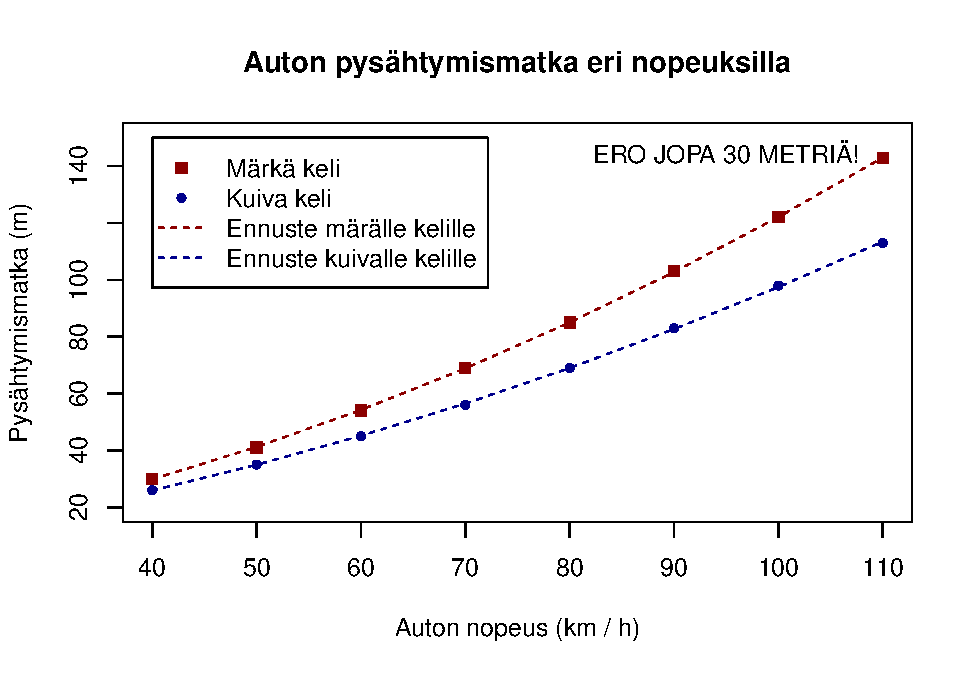
\includegraphics{R-ohjelmoinnin-perusteet_files/figure-latex/unnamed-chunk-114-1.pdf}
Kuvaajamme on nyt valmis!

\hypertarget{kuvaajien-piirtuxe4minen-kuxe4ytuxe4nnuxf6ssuxe4}{%
\section{Kuvaajien piirtäminen käytännössä}\label{kuvaajien-piirtuxe4minen-kuxe4ytuxe4nnuxf6ssuxe4}}

Jos äskeisen esimerkin aikana tuntui siltä, että näimme paljon työtä ja saimme lopputulokseksi kuvaajan, joka ei oikeastaan edes näytä kovin hyvältä, olet aivan oikeassa. Kuvaajien rakentaminen itse R:n peruskomennoilla on raskasta, ja usein perusgrafiikkatoimintoja käytetään lähinnä omaan käyttöön tulevien kuvaajien piirtämiseen nopeasti. Peruskomennot on kuitenkin hyvä hallita, sillä niitä saattaa tarvita valmiilla työkaluilla tehtyjen kuvaajien muokkaamiseen. Varsinkin tekstin lisääminen, sekä akselien nimeäminen ja otsikon muuttaminen ovat hyviä taitoja osata.

R tarjoaa paljon valmiita työkaluja erilaisten kuvaajien piirtämiseen. Valitettavasti tällä kurssilla ei ole aikaa sukeltaa näiden työkalujen käyttöön, sillä ennen niiden käyttöä pitää ymmärtää enemmän R:n monimutkaisemmista tietorakenteista, joita käsitellään seuraavilla viikoilla. Inspiraatiota ja motivaatiota voi kuitenkin hakea esimerkiksi \href{https://www.r-graph-gallery.com/index.html}{R Graph Gallery}-sivulta tai \href{https://rpkgs.datanovia.com/ggpubr/index.html}{ggpubr-paketin ohjeista}.

\hypertarget{tests}{%
\chapter{Tilastollinen testaaminen}\label{tests}}

\hypertarget{testaamisen-periaatteita}{%
\section{Testaamisen periaatteita}\label{testaamisen-periaatteita}}

Tilastollisilla testeillä pyritään arvioimaan perusjoukkoa koskevien väiteiden paikkansapitävyyttä todennäköisyyslaskennan keinoin. Lähtökohtana on niin sanottu \textbf{nollahypoteesi} (\(H_0\)), joka yleensä vastaa tilannetta, jossa mahdolliset väitettä tukevat haivainnot ovat vain sattuman seurausta. Esimerkiksi jos tutkitaan onko jokin lääkeaine tehokas hoitokeino, voisi nollahypoteesi olla muotoa ``ei vaikutusta''. Nollahypoteesiin liittyy aina \textbf{vastahypoteesi} (\(H_1\)), joka yleensä nollahypoteesin vastakohta, ja vastaa mielenkiinnon kohteena olevaa väitettä (esim. ``on vaikutusta'').

Tilastolliset testit olettava nollahypoteesin olevan totta, jolloin epäuskottavat tulokset antavat aihetta epäillä nollahypoteesin mielekkyyttä. Testiin liittyy yleensä \textbf{testisuure}, joka on jokin aineistosta laskettu tunnusluku. Testisuureen jakauman perusteella voidaan arvioida todennäköisyyttä, että havaittu tulos olisi vain sattuman seurausta. Tätä todennäköisyyttä kutsutaan \textbf{p-arvoksi}. Perinteisesti tilastotieteessä asetetaan etukäteen jokin riskitaso (\(\alpha\)), ja jos saatu p-arvo on riskitasoa pienempi niin nollahypoteesi hylätään (yleensä \(\alpha = 0.05\)). Jos p-arvo on riskitasoa pienempi, niin havaintoa kutsutaan tilastollisesti merkitseväksi.

\hypertarget{t-test}{%
\section{t-testi}\label{t-test}}

Studentin t-testi on yksi tunnetuimmista tilastollisista testeistä. Se testaa muuttujien odotusarvoja.

Tarkastellaan R:n sisäistä dataa \texttt{sleep}, joka sisältää muutoksia oppilaiden unen määrässä (muuttuja \texttt{extra}, muutos unen määrässä tunneissa) kahdella eri lääkkeellä (muuttuja \texttt{group}). Jokainen oppilas kokeili kumpaakin lääkettä, muuttuja \texttt{ID} yksilöi oppilaat.

\hypertarget{yhden-otoksen-t-testi}{%
\subsection{Yhden otoksen t-testi}\label{yhden-otoksen-t-testi}}

Testaamme aluksi hypoteesia, että muutos unen määrässä lääkkeen käytön jälkeen on 0 (\(H_0 : \mu = 0\)). Funktiota \texttt{t.test} voi käyttää monella tapaa. Tässä esimerkissä annamme funktiolle kaavan \texttt{extra\ \textasciitilde{}\ 1}, eli ns. \texttt{formula}-objektin ensimmäisenä argumenttina, joka on osa R:n syntaksia tilastollisten mallien ja riippuvuusrakenteiden määrittellyyn. Kaava määrittelee, että \texttt{\textasciitilde{}}-merkin vasen puoli on vastemuuttuja, ja oikea puoli sisältää selittävät muuttujat. Koska emme tee testiä minkään toisen muuttujan suhteen, niin kaavan oikean puoli on vain luku 1, joka R:n syntaksissa tarkoittaa, että se on vakio. Tämä ei siis tarkoita esimerkiksi sitä, että nollahypoteesimme olisi, että muutos unen määrässä olisi 1 tunti. Nollahypoteesin mukainen odotusarvo määritellään argumentilla \texttt{mu}, joka yhden otoksen testissä saa oletusarvon 0.

\begin{Shaded}
\begin{Highlighting}[]
\CommentTok{\# One sample test}
\NormalTok{tt1 }\OtherTok{\textless{}{-}} \FunctionTok{t.test}\NormalTok{(extra }\SpecialCharTok{\textasciitilde{}} \DecValTok{1}\NormalTok{, }\AttributeTok{data =}\NormalTok{ sleep)}
\NormalTok{tt1}
\end{Highlighting}
\end{Shaded}

\begin{verbatim}
## 
##  One Sample t-test
## 
## data:  extra
## t = 3.413, df = 19, p-value = 0.002918
## alternative hypothesis: true mean is not equal to 0
## 95 percent confidence interval:
##  0.5955845 2.4844155
## sample estimates:
## mean of x 
##      1.54
\end{verbatim}

Tuloksena saamme t-testisuureen arvon, vapausasteet sekä testin p-arvon. Koska p-arvo on pieni (perinteisesti rajana käytetään lukua 0.05, mutta tämä vaihtelee tieteenalasta riippuen) niin nollahypoteesi hylätään, eli testin mukaan muutos unen määrässä poikkeaa tilastollisesti merkitsevästi nollasta kumpaa tahansa lääkettä käytettäessä.

Testiin liittyvät tunnusluvut saamme eriteltyä tulosobjektista \texttt{tt1} seuraavasti:

\begin{Shaded}
\begin{Highlighting}[]
\CommentTok{\# Test statistic}
\NormalTok{tt1}\SpecialCharTok{$}\NormalTok{statistic}
\end{Highlighting}
\end{Shaded}

\begin{verbatim}
##        t 
## 3.412965
\end{verbatim}

\begin{Shaded}
\begin{Highlighting}[]
\CommentTok{\# Degrees of freedom}
\NormalTok{tt1}\SpecialCharTok{$}\NormalTok{parameter}
\end{Highlighting}
\end{Shaded}

\begin{verbatim}
## df 
## 19
\end{verbatim}

\begin{Shaded}
\begin{Highlighting}[]
\CommentTok{\# p{-}value}
\NormalTok{tt1}\SpecialCharTok{$}\NormalTok{p.value}
\end{Highlighting}
\end{Shaded}

\begin{verbatim}
## [1] 0.00291762
\end{verbatim}

\hypertarget{kahden-otoksen-t-testi}{%
\subsection{Kahden otoksen t-testi}\label{kahden-otoksen-t-testi}}

Entäpä jos haluammekin testata hypoteesia, että kumpikin lääke vaikuttaa samalla tavalla unen määrään (\(H_0 : \mu_1 = \mu_2\))? Voimme tässäkin tapauksessa käyttää \texttt{formula}-syntaksia hyödyksi. Vakion 1 sijaan sijoitamme nyt lääkettä vastaavan muuttujan \texttt{group} kaavassa \texttt{\textasciitilde{}}-merkin oikealle puolelle.

\begin{Shaded}
\begin{Highlighting}[]
\NormalTok{tt2 }\OtherTok{\textless{}{-}} \FunctionTok{t.test}\NormalTok{(extra }\SpecialCharTok{\textasciitilde{}}\NormalTok{ group, }\AttributeTok{data =}\NormalTok{ sleep)}
\NormalTok{tt2}
\end{Highlighting}
\end{Shaded}

\begin{verbatim}
## 
##  Welch Two Sample t-test
## 
## data:  extra by group
## t = -1.8608, df = 17.776, p-value = 0.07939
## alternative hypothesis: true difference in means between group 1 and group 2 is not equal to 0
## 95 percent confidence interval:
##  -3.3654832  0.2054832
## sample estimates:
## mean in group 1 mean in group 2 
##            0.75            2.33
\end{verbatim}

Testiobjektin sisältö vastaa yhden otoksen testiä suurimmilta osin. Näämme, että testin tulos ei tällä kertaa ollut tilastollisesti merkitsevä (merkitsevyystasolla 0.05) eli testin mukaan ei ole näyttöä siitä, että lääkkeet vaikuttaisivat eri tavalla unen määrään, jolloin nollahypoteesia ei hylätä.

Tarkkasilmäinen lukija saattoi kuitenkin huomata, että tämä testi ei aivan vastaa tarkoitusta, sillä \texttt{sleep}-aineistossa jokainen koehenkilö kokeili kumpaakin lääkettä, jolloin oikea tapa olisi testata lääkkeiden vaikutuksen erotusta, mikä tehdäänkin seuraavaksi.

\hypertarget{parittaisten-otosten-t-testi}{%
\subsection{Parittaisten otosten t-testi}\label{parittaisten-otosten-t-testi}}

Jotta mittausparit tulevat otettua huomioon testissä, on \texttt{t.test}-funktiolle annettava argumentti \texttt{paired\ =\ TRUE}. Tässä testissä nollahypoteesi on, että lääkkeiden vaikutuksen erotuksen odotusarvo on 0 (\(H_0 : \mu_d = 0\)).

\begin{Shaded}
\begin{Highlighting}[]
\NormalTok{tt3 }\OtherTok{\textless{}{-}} \FunctionTok{t.test}\NormalTok{(extra }\SpecialCharTok{\textasciitilde{}}\NormalTok{ group, }\AttributeTok{data =}\NormalTok{ sleep, }\AttributeTok{paired =} \ConstantTok{TRUE}\NormalTok{)}
\NormalTok{tt3}
\end{Highlighting}
\end{Shaded}

\begin{verbatim}
## 
##  Paired t-test
## 
## data:  extra by group
## t = -4.0621, df = 9, p-value = 0.002833
## alternative hypothesis: true difference in means is not equal to 0
## 95 percent confidence interval:
##  -2.4598858 -0.7001142
## sample estimates:
## mean of the differences 
##                   -1.58
\end{verbatim}

Tällä kertaa tulos on taas tilastollisesti merkitsevä, eli lääkkeiden vaikutuksessa unen määrään on tilastollisesti merkitsevä ero, jolloin nollahypoteesi hylätään.

\hypertarget{chi-squared-test}{%
\section{Khiin neliö -testi}\label{chi-squared-test}}

Kahden kategorisen muuttujan riippuvuuden tutkimiseen voidaan käyttää khiin neliö -testiä. Tyypillisesti halutaan verrata jotain ryhmien välisiä eroja, kuten puoluekannatusta alueittain tai sukupuolten suhteen. Testin ideana on verrata havaittua ristiintaulukkoa nollahypoteesin mukaiseen ristiintaulukkoon, jossa muuttujien välillä ei ole lainkaan riippuvuutta. Khiin neliö -testin testisuure perustuu näiden kahden taulukon eroihin.

Tarkastellaan Yhdysvaltalaista kyselytutkimusaineistoa, joka sisältää tiedon henkilön puoluekannatuksesta ja sukupuolesta. Tutkitaan khiin neliö -testin avulla, riippuuko puoluekannatus sukupuolesta. R:ssä tämä voidaan tehdä funktiolla \texttt{chisq.test}.

\begin{Shaded}
\begin{Highlighting}[]
\DocumentationTok{\#\# From Agresti(2007) p.39}
\NormalTok{M }\OtherTok{\textless{}{-}} \FunctionTok{as.table}\NormalTok{(}\FunctionTok{rbind}\NormalTok{(}\FunctionTok{c}\NormalTok{(}\DecValTok{762}\NormalTok{, }\DecValTok{327}\NormalTok{, }\DecValTok{468}\NormalTok{), }\FunctionTok{c}\NormalTok{(}\DecValTok{484}\NormalTok{, }\DecValTok{239}\NormalTok{, }\DecValTok{477}\NormalTok{)))}
\FunctionTok{dimnames}\NormalTok{(M) }\OtherTok{\textless{}{-}} \FunctionTok{list}\NormalTok{(}\AttributeTok{gender =} \FunctionTok{c}\NormalTok{(}\StringTok{"F"}\NormalTok{, }\StringTok{"M"}\NormalTok{),}
                    \AttributeTok{party =} \FunctionTok{c}\NormalTok{(}\StringTok{"Democrat"}\NormalTok{, }\StringTok{"Independent"}\NormalTok{, }\StringTok{"Republican"}\NormalTok{))}
\NormalTok{(Xsq }\OtherTok{\textless{}{-}} \FunctionTok{chisq.test}\NormalTok{(M))  }\CommentTok{\# Prints test summary}
\end{Highlighting}
\end{Shaded}

\begin{verbatim}
## 
##  Pearson's Chi-squared test
## 
## data:  M
## X-squared = 30.07, df = 2, p-value = 2.954e-07
\end{verbatim}

\begin{Shaded}
\begin{Highlighting}[]
\NormalTok{Xsq}\SpecialCharTok{$}\NormalTok{observed   }\CommentTok{\# observed counts (same as M)}
\end{Highlighting}
\end{Shaded}

\begin{verbatim}
##       party
## gender Democrat Independent Republican
##      F      762         327        468
##      M      484         239        477
\end{verbatim}

\begin{Shaded}
\begin{Highlighting}[]
\NormalTok{Xsq}\SpecialCharTok{$}\NormalTok{expected   }\CommentTok{\# expected counts under the null}
\end{Highlighting}
\end{Shaded}

\begin{verbatim}
##       party
## gender Democrat Independent Republican
##      F 703.6714    319.6453   533.6834
##      M 542.3286    246.3547   411.3166
\end{verbatim}

\begin{Shaded}
\begin{Highlighting}[]
\NormalTok{Xsq}\SpecialCharTok{$}\NormalTok{residuals  }\CommentTok{\# Pearson residuals}
\end{Highlighting}
\end{Shaded}

\begin{verbatim}
##       party
## gender   Democrat Independent Republican
##      F  2.1988558   0.4113702 -2.8432397
##      M -2.5046695  -0.4685829  3.2386734
\end{verbatim}

\begin{Shaded}
\begin{Highlighting}[]
\NormalTok{Xsq}\SpecialCharTok{$}\NormalTok{stdres     }\CommentTok{\# standardized residuals}
\end{Highlighting}
\end{Shaded}

\begin{verbatim}
##       party
## gender   Democrat Independent Republican
##      F  4.5020535   0.6994517 -5.3159455
##      M -4.5020535  -0.6994517  5.3159455
\end{verbatim}

Koska testin p-arvo on pieni, niin nollahypoteesi hylätään ja todetaan, että puoluekannatus riippuu tilastollisesti merkitsevästi sukupuolesta. Testin luotettavuuden kannalta on kuitenkin hyvä huomioida, että testiin liittyy oletuksia, jotka koskevat odotettuja frekvenssejä (eli nollahypoteesin mukaisen ristiintaulukon frekvenssejä). Tyypillisesti vaaditaan, että odotetun frekvenssin on oltava vähintään 5 vähintään 80\%:ssa taulukon soluista, eikä yhdenkään solun odotettu frekvenssi ole alle 1. Tarkistetaan oletukset edellisen esimerkin tapauksessa:

\begin{Shaded}
\begin{Highlighting}[]
\FunctionTok{all}\NormalTok{(Xsq}\SpecialCharTok{$}\NormalTok{expected }\SpecialCharTok{\textgreater{}=} \DecValTok{1}\NormalTok{)}
\end{Highlighting}
\end{Shaded}

\begin{verbatim}
## [1] TRUE
\end{verbatim}

\begin{Shaded}
\begin{Highlighting}[]
\FunctionTok{mean}\NormalTok{(Xsq}\SpecialCharTok{$}\NormalTok{expected }\SpecialCharTok{\textgreater{}=} \DecValTok{5}\NormalTok{) }\SpecialCharTok{\textgreater{}=} \FloatTok{0.80}
\end{Highlighting}
\end{Shaded}

\begin{verbatim}
## [1] TRUE
\end{verbatim}

Oletukset ovat tältä osin kunnossa. Edellä funktio \texttt{all} ottaa syötteenään loogisen vektorin ja palauttaa \texttt{TRUE} jos syötteen kaikki alkiot ovat \texttt{TRUE}. Muutoin funktio palauttaa \texttt{FALSE}.

\hypertarget{anova}{%
\section{Varianssianalyysi}\label{anova}}

Varianssianalyysin voidaan ajatella olevan t-testin yleistys, jossa yhden tai kahden odotusarvon sijaan verrataankin kerralla useamman ryhmän odotusarvoja keskenään. Menetelmä saa nimensä siitä, että sen testisuure perustuu kiinnostuksen kohteena olevan muuttujan kokonaisvaihtelun jakamiseen verratavien ryhmien sisäiseen vaihteluun ja niiden väliseen vaihteluun. Koska harjoitusaineistossa \texttt{study\_data} ei vielä ole kategorista muuttujaa, jossa on vähintään kolme kategoriaa, niin luodaan sellainen.

\begin{Shaded}
\begin{Highlighting}[]
\CommentTok{\# create a new categorical variable called age\_group}
\CommentTok{\#3,5,6 =\textgreater{} ryhmä 1}
\CommentTok{\#2,4,8 =\textgreater{} ryhmä 2}
\CommentTok{\#1,7   =\textgreater{} ryhmä 3}
\CommentTok{\# vaste: weight}
\NormalTok{study\_data}\SpecialCharTok{$}\NormalTok{age\_group }\OtherTok{\textless{}{-}} \FunctionTok{c}\NormalTok{(}\StringTok{"3"}\NormalTok{, }\StringTok{"2"}\NormalTok{, }\StringTok{"1"}\NormalTok{, }\StringTok{"2"}\NormalTok{, }\StringTok{"1"}\NormalTok{, }\StringTok{"1"}\NormalTok{, }\StringTok{"3"}\NormalTok{, }\StringTok{"2"}\NormalTok{)}
\NormalTok{study\_data}\SpecialCharTok{$}\NormalTok{fage\_group }\OtherTok{\textless{}{-}} \FunctionTok{factor}\NormalTok{(study\_data}\SpecialCharTok{$}\NormalTok{age\_group)}
\end{Highlighting}
\end{Shaded}

Hypoteesit ovat:
- \(H_0\): Ryhmien odotusarvot ovat samat tarkasteltavan muuttujan suhteen (\(\mu_1 = \mu_2 = \dots = \mu_n\)),
- \(H_1\): Ryhmien odotusarvoissa on eroa tarkasteltavan muuttujan suhteen (\(\mu_i \ne \mu_j\) ainakin joillekin \(i \ne j\)).

\begin{Shaded}
\begin{Highlighting}[]
\CommentTok{\# conduct Analysis of Variance (ANOVA) for study\_data}
\CommentTok{\# we test if averages of height differ between age groups}
\FunctionTok{summary}\NormalTok{(}\FunctionTok{aov}\NormalTok{(height }\SpecialCharTok{\textasciitilde{}}\NormalTok{ fage\_group, }\AttributeTok{data =}\NormalTok{ study\_data))}
\end{Highlighting}
\end{Shaded}

\begin{verbatim}
##             Df Sum Sq Mean Sq F value Pr(>F)
## fage_group   2  198.7   99.34   1.097  0.417
## Residuals    4  362.4   90.60               
## 1 observation deleted due to missingness
\end{verbatim}

\begin{Shaded}
\begin{Highlighting}[]
\FunctionTok{summary}\NormalTok{(}\FunctionTok{aov}\NormalTok{(height }\SpecialCharTok{\textasciitilde{}}\NormalTok{ fage\_group, }\AttributeTok{data =}\NormalTok{ study\_data[}\FunctionTok{rep}\NormalTok{(}\DecValTok{1}\SpecialCharTok{:}\DecValTok{8}\NormalTok{,}\DecValTok{3}\NormalTok{),])) }\CommentTok{\# the same data three times}
\end{Highlighting}
\end{Shaded}

\begin{verbatim}
##             Df Sum Sq Mean Sq F value Pr(>F)  
## fage_group   2  596.1   298.0   4.934 0.0196 *
## Residuals   18 1087.2    60.4                 
## ---
## Signif. codes:  0 '***' 0.001 '**' 0.01 '*' 0.05 '.' 0.1 ' ' 1
## 3 observations deleted due to missingness
\end{verbatim}

\hypertarget{levene}{%
\section{Levenen testi}\label{levene}}

Levenen testillä tutkitaan ovatko jonkin muuttujan varianssit samat kahdessa tai useammassa ryhmässä. Testiä ei ole toteutettu perus R:ssä, mutta se on saatavilla Rcourse-paketin kautta funktiossa \texttt{leveneTest}. Testin nollahypoteesi on, että muuttujan varianssit ovat samat joka ryhmässä.

Selvitetään onko harjoitusaineiston \texttt{study\_data} muuttujan \texttt{height} varianssissa eroa eri ikäryhmien välillä (\texttt{fage\_group}) Levenen testillä.

\begin{Shaded}
\begin{Highlighting}[]
\FunctionTok{leveneTest}\NormalTok{(height }\SpecialCharTok{\textasciitilde{}}\NormalTok{ fage\_group, }\AttributeTok{data =}\NormalTok{ study\_data)}
\end{Highlighting}
\end{Shaded}

\begin{verbatim}
## Levene's Test for Homogeneity of Variance (center = median)
##       Df F value Pr(>F)
## group  2  0.5597 0.6105
##        4
\end{verbatim}

Testin p-arvo löytyy sarakkeesta \texttt{Pr(\textgreater{}F)}, ja se on noin \(0.61\). Testin mukaan muuttujan varianssit ovat siis samat joka ryhmässä, ja nollahypoteesi jää voimaan.

\hypertarget{shapiro}{%
\section{Shapiro-Wilk -testi}\label{shapiro}}

Shapiro-Wilk -testillä tutkitaan onko jokin muuttuja normaalijakautunut. Testi löytyy funktiosta \texttt{shapiro.test}, ja se ottaa argumenttinaan yhden muuttujan havainnot vektorina. Funktiolla ei voi siis suoraan testata esimerkiksi sitä, onko muuttuja normaalijakautunut joissakin osaryhmissä, vaan aineisto on ensin jaettava sopiviin osiin. Testin nollahypoteesi on, että muuttuja on normaalijakautunut.

Tarkastellaan jälleen harjoitusaineistoa \texttt{study\_data} ja testataan muuttujan \texttt{height} normaalisuutta.

\begin{Shaded}
\begin{Highlighting}[]
\FunctionTok{shapiro.test}\NormalTok{(study\_data}\SpecialCharTok{$}\NormalTok{height)}
\end{Highlighting}
\end{Shaded}

\begin{verbatim}
## 
##  Shapiro-Wilk normality test
## 
## data:  study_data$height
## W = 0.96985, p-value = 0.8973
\end{verbatim}

Testin p-arvon voi lukea kohdasta \texttt{p-value} ja se on aineistolle noin \(0.90\), eli \texttt{height}-muuttuja on testin mukaan normaalijakautunut, ja nollahypoteesi jää voimaan.

\hypertarget{linear_models}{%
\chapter{Lineaariset mallit}\label{linear_models}}

Lineaarisessa mallissa eli lineaarisessa regressiossa tavoite on arvioida vastemuuttujan lineaarista riippuvuutta selittävistä muuttujista. Käytetään esimerkkinä R:n sisäistä datasettiä cars, joka sisältää 50 auton nopeudet ja pysähtymismatkat. Tavoitteena on tutkia, miten auton pysähtymismatka riippuu auton nopeudesta.

\hypertarget{teoria}{%
\section{Teoria}\label{teoria}}

Yksinkertaisin mahdollinen lineaarinen regressiomalli on:

\[ y = \beta_0 + \beta_1 x_1 + \epsilon \]

\begin{itemize}
\tightlist
\item
  \(y\) on \textbf{vastemuuttuja}, eli tässä auton pysähtymismatka
\item
  \(\beta_0\) on ns. \textbf{vakiotermi} eli käyrän \(y\)-akselin leikkauskohta
\item
  \(\beta_1\) on selittävän muuttujan eli auton nopeuden \textbf{regressiokerroin}
\item
  \(x_1\) on selittävä muuttuja eli auton nopeus
\item
  \(\epsilon\) on \textbf{residuaali} (jäännösvirhe)
\end{itemize}

Mallissa siis oletetaan, että auton pysähtymismatka nopeudella 0 km/h on \(\beta_0\) ja kasvaa \(\beta_1\) verran, kun nopeus kasvaa 1 km/h. Lisäksi mukana on virhetermi \(\epsilon\), joka selittää satunnaisen vaihtelun tuloksissa lineaarisen käyrän ympärillä.

Jos malliin halutaan lisätä selittäviä muuttujia, kuten auton jarrujen kunto (\(x_2\)) tai sääolosuhteet (\(x_3\)), malli näyttää tältä:

\[ y = \beta_0 + \beta_1 x_1 + \beta_2 x_2 + \beta_3 x_3 + ... + \epsilon \]

Eli jokaiselle selittävälle muuttujalle annetaan oma regressiokerroin.

\hypertarget{esimerkki}{%
\section{Esimerkki}\label{esimerkki}}

Muutetaan ensin cars-datasetin muuttujat meille tuttuihin yksiköihin, ja piirretään hajontakuvio havainnoista:

\begin{Shaded}
\begin{Highlighting}[]
\CommentTok{\# Change to SI units}
\NormalTok{cars}\SpecialCharTok{$}\NormalTok{speed }\OtherTok{\textless{}{-}}\NormalTok{ cars}\SpecialCharTok{$}\NormalTok{speed }\SpecialCharTok{*} \FloatTok{1.60934}
\NormalTok{cars}\SpecialCharTok{$}\NormalTok{dist }\OtherTok{\textless{}{-}}\NormalTok{ cars}\SpecialCharTok{$}\NormalTok{dist }\SpecialCharTok{*} \FloatTok{0.0254}
\CommentTok{\# Scatter plot}
\FunctionTok{plot}\NormalTok{(cars}\SpecialCharTok{$}\NormalTok{speed, cars}\SpecialCharTok{$}\NormalTok{dist,}
     \AttributeTok{xlab =} \StringTok{"Speed (km/h)"}\NormalTok{, }\AttributeTok{ylab =} \StringTok{"Distance (m)"}\NormalTok{,}
     \AttributeTok{main =} \StringTok{"Stopping distances of cars"}\NormalTok{) }
\end{Highlighting}
\end{Shaded}

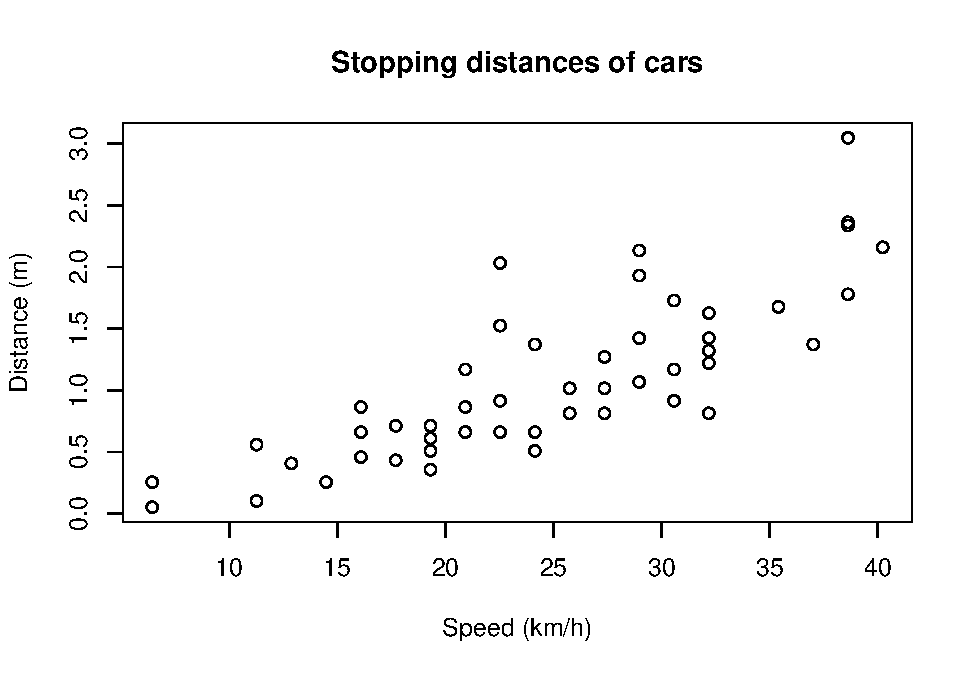
\includegraphics{R-ohjelmoinnin-perusteet_files/figure-latex/unnamed-chunk-128-1.pdf}

Autojen välillä on eroja, mutta kuten voi odottaa, suuremmilla nopeuksilla auton pysähtymismatka kasvaa. Käytetään seuraavaksi R:n funktiota \texttt{lm}, jolla voidaan sovittaa dataan lineaarinen malli:

\begin{Shaded}
\begin{Highlighting}[]
\NormalTok{model }\OtherTok{\textless{}{-}} \FunctionTok{lm}\NormalTok{(dist }\SpecialCharTok{\textasciitilde{}}\NormalTok{ speed, }\AttributeTok{data =}\NormalTok{ cars)}
\NormalTok{model}\SpecialCharTok{$}\NormalTok{coefficients}
\end{Highlighting}
\end{Shaded}

\begin{verbatim}
## (Intercept)       speed 
## -0.44650901  0.06206469
\end{verbatim}

\texttt{lm}-funktiolle annetaan ensimmäiseksi argumentiksi lineaarisen mallin kaava, jossa \texttt{\textasciitilde{}} korvaa yllä nähdyn yhtäkuin-merkin. HUOM: vakiotermi on automaattisesti mukana, eli sitä ei tarvitse kirjata erikseen. Lisäksi täytyy antaa argumentti \texttt{data}, jonka tulee olla datakehikko, josta kaavassa olevat muuttujat löytyvät.

Lineaarisesta mallista saadaan irti paljon tietoa, tärkeimpinä mallin regressiokertoimet (coefficients). Yllä olevista kertoimista voidaan päätellä, että kun auton nopeus nousee 1 km/h niin sen pysähtymismatka kasvaa noin 0.06 m, ja odotettu kasvukäyrä leikkaa y-akselin -0.4 m kohdalla. Voimme piirtää tämän käyrän kuvaajaan \texttt{abline}-funktion avulla, antamalla sille mallin kertoimet:

\begin{Shaded}
\begin{Highlighting}[]
\FunctionTok{plot}\NormalTok{(cars}\SpecialCharTok{$}\NormalTok{speed, cars}\SpecialCharTok{$}\NormalTok{dist,}
     \AttributeTok{xlab =} \StringTok{"Speed (km/h)"}\NormalTok{, }\AttributeTok{ylab =} \StringTok{"Distance (m)"}\NormalTok{,}
     \AttributeTok{main =} \StringTok{"Stopping distances of cars"}\NormalTok{)}
\FunctionTok{abline}\NormalTok{(}\AttributeTok{a =}\NormalTok{ model}\SpecialCharTok{$}\NormalTok{coefficients[}\DecValTok{1}\NormalTok{], }\AttributeTok{b =}\NormalTok{ model}\SpecialCharTok{$}\NormalTok{coefficients[}\DecValTok{2}\NormalTok{])}
\end{Highlighting}
\end{Shaded}

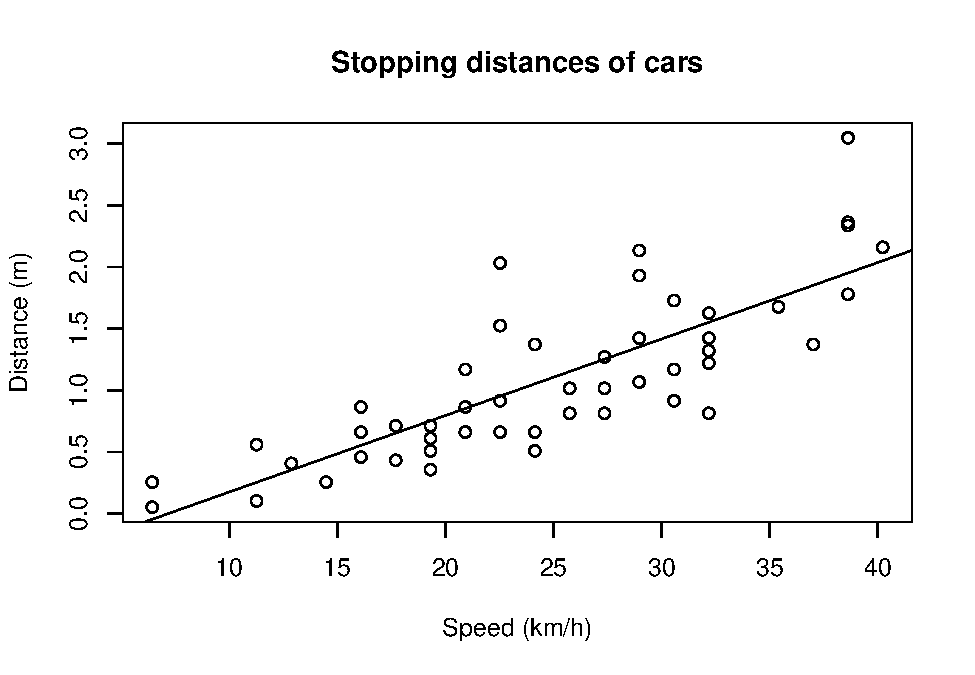
\includegraphics{R-ohjelmoinnin-perusteet_files/figure-latex/unnamed-chunk-130-1.pdf}

\hypertarget{tarkempia-tietoja-mallista}{%
\section{Tarkempia tietoja mallista}\label{tarkempia-tietoja-mallista}}

Muihin mallin tietoihin pääsee käsiksi \texttt{summary}-funktion avulla, joko tulostamalla tuloksen konsoliin, tai sijoittamalla sen muuttujaan, josta voi etsiä mallin tietoja.

\begin{Shaded}
\begin{Highlighting}[]
\CommentTok{\# Print summary information}
\FunctionTok{summary}\NormalTok{(model)}
\end{Highlighting}
\end{Shaded}

\begin{verbatim}
## 
## Call:
## lm(formula = dist ~ speed, data = cars)
## 
## Residuals:
##      Min       1Q   Median       3Q      Max 
## -0.73835 -0.24194 -0.05771  0.23405  1.09731 
## 
## Coefficients:
##              Estimate Std. Error t value Pr(>|t|)    
## (Intercept) -0.446509   0.171664  -2.601   0.0123 *  
## speed        0.062065   0.006558   9.464 1.49e-12 ***
## ---
## Signif. codes:  0 '***' 0.001 '**' 0.01 '*' 0.05 '.' 0.1 ' ' 1
## 
## Residual standard error: 0.3906 on 48 degrees of freedom
## Multiple R-squared:  0.6511, Adjusted R-squared:  0.6438 
## F-statistic: 89.57 on 1 and 48 DF,  p-value: 1.49e-12
\end{verbatim}

\begin{Shaded}
\begin{Highlighting}[]
\CommentTok{\# Save summary and access specific information}
\NormalTok{s }\OtherTok{\textless{}{-}} \FunctionTok{summary}\NormalTok{(model)}
\NormalTok{s}\SpecialCharTok{$}\NormalTok{r.squared}
\end{Highlighting}
\end{Shaded}

\begin{verbatim}
## [1] 0.6510794
\end{verbatim}

\texttt{summary} kertoo mm. kertoimien arvojen lisäksi niiden saamat p-arvot kohdassa (Pr \textgreater{} \textbar t\textbar), sekä mallin selitysasteen (merkintätapa johtuu siitä, että p-arvot tulevat t-testeistä). Tässä tapauksessa muuttujan speed p-arvo on hyvin pieni, joten voimme todeta suurella varmuudella, että autojen pysähtymismatka riippuu (lineaarisesti) auton nopeudesta. \(R^2\) eli R-squared kertoo, kuinka suuren osuuden pysähtymismatkojen varianssista auton nopeus selittää.

Mallin regressiokerrointen estimoitu kovarianssimatriisi saadaan funktiolla \texttt{vcov} (variance-covariance matrix). Kertoimien keskivirheet saadaan tästä edelleen helposti matriisin diagonaalin neliöjuurina (funktiot \texttt{diag} ja \texttt{sqrt}):

\begin{Shaded}
\begin{Highlighting}[]
\CommentTok{\# Covariance matrix of the regression coefficients}
\FunctionTok{vcov}\NormalTok{(model)}
\end{Highlighting}
\end{Shaded}

\begin{verbatim}
##              (Intercept)         speed
## (Intercept)  0.029468659 -1.065882e-03
## speed       -0.001065882  4.300714e-05
\end{verbatim}

\begin{Shaded}
\begin{Highlighting}[]
\CommentTok{\# Standard errors only}
\FunctionTok{sqrt}\NormalTok{(}\FunctionTok{diag}\NormalTok{(}\FunctionTok{vcov}\NormalTok{(model)))}
\end{Highlighting}
\end{Shaded}

\begin{verbatim}
## (Intercept)       speed 
## 0.171664380 0.006557983
\end{verbatim}

\hypertarget{ennustaminen}{%
\section{Ennustaminen}\label{ennustaminen}}

Kun lineaarinen malli on estimoitu, sen perusteella voidaan myös ennustaa arvoja uusille havainnoille. Tämä tapahtuu \texttt{predict}-funktiolla, jolle annetaan malli, sekä datakehikko, joka sisältää ne selittäjien arvot, joille halutaan laskea ennusteet. Tämä datakehikko voi sisältää useita rivejä, jolloin ennuste lasketaan joka riville. Ennustetaan edellisen mallin perusteella pysähtymismatka autolle kolmella uudella nopeudella ja lisätään ne edelliseen kuvaajaan punaisilla rukseilla:

\begin{Shaded}
\begin{Highlighting}[]
\CommentTok{\# Create data frame with new speed values}
\NormalTok{new\_data }\OtherTok{\textless{}{-}} \FunctionTok{data.frame}\NormalTok{(}\AttributeTok{speed =} \FunctionTok{c}\NormalTok{(}\DecValTok{25}\NormalTok{, }\DecValTok{15}\NormalTok{, }\DecValTok{38}\NormalTok{))}
\CommentTok{\# Create dist column by predicting from linear model}
\NormalTok{new\_data}\SpecialCharTok{$}\NormalTok{dist }\OtherTok{\textless{}{-}} \FunctionTok{predict}\NormalTok{(model, }\AttributeTok{newdata =}\NormalTok{ new\_data)}

\CommentTok{\# Add points to previous plot}
\FunctionTok{plot}\NormalTok{(cars}\SpecialCharTok{$}\NormalTok{speed, cars}\SpecialCharTok{$}\NormalTok{dist,}
     \AttributeTok{xlab =} \StringTok{"Speed (km/h)"}\NormalTok{, }\AttributeTok{ylab =} \StringTok{"Distance (m)"}\NormalTok{,}
     \AttributeTok{main =} \StringTok{"Stopping distances of cars"}\NormalTok{)}
\FunctionTok{abline}\NormalTok{(}\AttributeTok{a =}\NormalTok{ model}\SpecialCharTok{$}\NormalTok{coefficients[}\DecValTok{1}\NormalTok{], }\AttributeTok{b =}\NormalTok{ model}\SpecialCharTok{$}\NormalTok{coefficients[}\DecValTok{2}\NormalTok{])}
\FunctionTok{points}\NormalTok{(new\_data}\SpecialCharTok{$}\NormalTok{speed, new\_data}\SpecialCharTok{$}\NormalTok{dist, }\AttributeTok{pch =} \DecValTok{4}\NormalTok{, }\AttributeTok{col =} \StringTok{"red"}\NormalTok{)}
\end{Highlighting}
\end{Shaded}

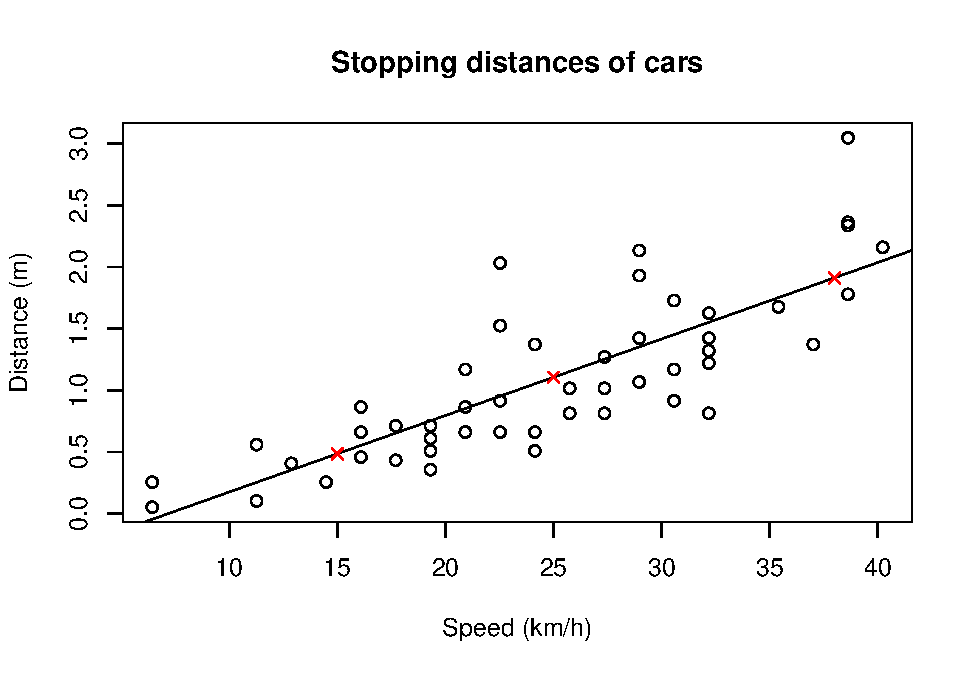
\includegraphics{R-ohjelmoinnin-perusteet_files/figure-latex/unnamed-chunk-133-1.pdf}

Kuten huomataan, ennustetut arvot ovat täsmälleen käyrän päällä.

\hypertarget{korrelaatio}{%
\section{Korrelaatio}\label{korrelaatio}}

Korrelaatio on lineaarisen regression ohella tapa mitata kahden muuttujan välistä riippuvuutta. Korrelaatiolle on monia erilaisia mittareita, joista yleisimmät ovat Pearsonin korrelaatiokerroin, joka mittaa kahden muuttujan välistä lineaarista riippuvuutta ja Spearmanin järjestyskorrelaatiokerroin, joka mittaa kahden muuttujan välistä riippuvuutta ilman lineaarisuusoletusta, mutta olettaa kuitenkin monotonisen riippuvuuden. HUOM: korrelaatio ei ota kantaa siihen, kuinka vahva riippuvuus on (käyrän jyrkkyys), vaan pelkästään siihen, kuinka systemaattinen riippuvuus on. Kummatkin korrelaatiokertoimet saavat arvoja väliltä {[}-1, 1{]}, jossa -1 on täydellinen negatiivinen korrelaatio (toisen muuttujan kasvaessa toinen aina pienenee) ja 1 on täydellinen positiivinen korrelaatio.

Korrelaation kahden vektorin välillä voi R:ssä laskea funktiolla \texttt{cor}. Otetaan esimerkiksi R:n sisäinen datasetti Indometh, jossa on mitattu indometasiinin farmakokinetiikkaa, ja selvitetään ajan ja indometasiinin konsentraation väliselle riippuvuudelle Pearsonin ja Spearmanin korrelaatiokertoimet. Piirretään sen jälkeen hajontakuvio mittaustuloksista ja lisätään kuvaajaan alaotsikoksi korrelaatiokertoimet. Tutustumme samalla funktioon \texttt{round}, jolla voi pyöristää lukuja halutulle desimaalitarkkuudelle. Huomaa, että \texttt{round}-funktio pyöristää aina lähimpään parilliseen lukuun, esim. luku 0.5 pyöristyy lukuun 0, mutta 1.5 pyöristyy lukuun 2.

\begin{Shaded}
\begin{Highlighting}[]
\CommentTok{\# Pearson correlation}
\NormalTok{pearson }\OtherTok{\textless{}{-}} \FunctionTok{cor}\NormalTok{(Indometh}\SpecialCharTok{$}\NormalTok{time, Indometh}\SpecialCharTok{$}\NormalTok{conc, }\AttributeTok{method =} \StringTok{"pearson"}\NormalTok{)}
\CommentTok{\# Spearman correlation}
\NormalTok{spearman }\OtherTok{\textless{}{-}} \FunctionTok{cor}\NormalTok{(Indometh}\SpecialCharTok{$}\NormalTok{time, Indometh}\SpecialCharTok{$}\NormalTok{conc, }\AttributeTok{method =} \StringTok{"spearman"}\NormalTok{)}
\CommentTok{\# Scatter plot}
\FunctionTok{plot}\NormalTok{(Indometh}\SpecialCharTok{$}\NormalTok{time, Indometh}\SpecialCharTok{$}\NormalTok{conc,}
     \AttributeTok{xlab =} \StringTok{"Time"}\NormalTok{, }\AttributeTok{ylab =} \StringTok{"Concetration"}\NormalTok{,}
     \AttributeTok{main =} \StringTok{"Pharmacokinetics of indometacin"}\NormalTok{)}

\CommentTok{\# Paste concatenates strings}
\NormalTok{subtitle }\OtherTok{\textless{}{-}} \FunctionTok{paste}\NormalTok{(}\StringTok{"Pearson correlation:"}\NormalTok{, }\FunctionTok{round}\NormalTok{(pearson, }\AttributeTok{digits =} \DecValTok{2}\NormalTok{),}
                  \StringTok{"Spearman correlation:"}\NormalTok{, }\FunctionTok{round}\NormalTok{(spearman, }\AttributeTok{digits =} \DecValTok{2}\NormalTok{))}
\CommentTok{\# Add subtitle to plot}
\FunctionTok{mtext}\NormalTok{(subtitle)}
\end{Highlighting}
\end{Shaded}

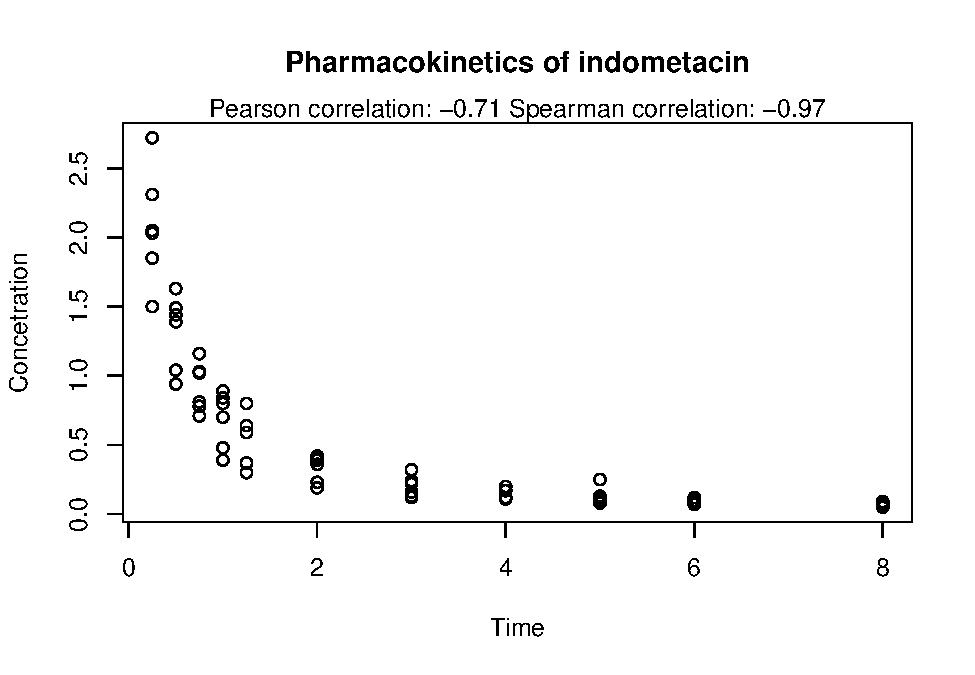
\includegraphics{R-ohjelmoinnin-perusteet_files/figure-latex/unnamed-chunk-134-1.pdf}

Tässä esimerkissä nähdään hyvin Pearsonin ja Spearmanin korrelaatiokertoimien ero. Koska Indometasiinin konsentraatio laskee eksponentiaalisesti, ei lineaarisesti, Pearsonin korrelaatiokerroin on ``vain'' -0.7, kun taas Spearmanin korrelaatiokerroin -0.97 vastaa lähes täydellistä negatiivista korrelaatiota.

\hypertarget{functions}{%
\chapter{Funktiot}\label{functions}}

Tässä kappaleessa tutustutaan omien funktioiden kirjoittamiseen ja pureudutaan sitä kautta syvemmälle R-funktioiden toimintaan.

\hypertarget{funktion-kuxe4site}{%
\section{Funktion käsite}\label{funktion-kuxe4site}}

Funktio on nimetty kokonaisuus järjesteltyä ja uudelleenkäytettävää koodia, jonka tarkoitus on suorittaa yksi tarkkaan määrätty tehtävä. Funktioilla on syöte (input) ja tulos (output). Funktion tehtävä on palauttaa (return) syötteen perusteella laskettu tulos. Alla olevassa kuvassa näkyvät funktion neljä osaa: nimi, syöte, toiminnallisuus ja tulos.

\includegraphics{files/06-functions/funktio_käsite.png}

Otetaan esimerkiksi kaksi funktiota: ``Keskiarvo'' ottaa syötteenä halutun määrän lukuja, ja laskee niiden keskiarvon. ``Vastinjuoste'' ottaa syötteenä DNA-juosteen ja palauttaa sen vastinjuosteen.

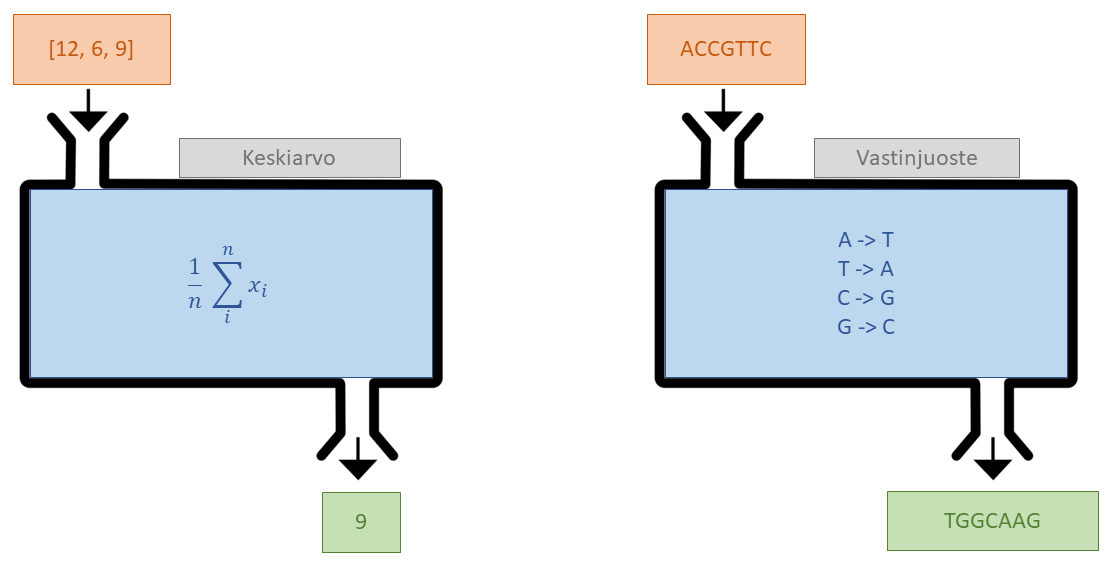
\includegraphics{files/06-functions/funktio_esimerkit.png}

Funktioilla voi olla myös erityyppisiä syötteitä. Voitaisiin esimerkiksi määritellä funktio, jolle annettaisiin syötteenä henkilön ikä, pituus, paino, sekä elintapatietoja, ja funktio laskisi näiden pohjalta eliniänodotteen. Yksittäisestä funktion syötteestä käytetään tavallisesti nimitystä ``argumentti''.

\hypertarget{r-funktiot}{%
\section{R-funktiot}\label{r-funktiot}}

\hypertarget{funktioiden-muxe4uxe4rittely}{%
\subsection{Funktioiden määrittely}\label{funktioiden-muxe4uxe4rittely}}

Tähän mennessä olemme jo käyttäneet monia R-funktioita, eikä meidän ole tarvinnut miettiä niiden toimintaa kovin syvällisesti. Mahdolliset virhetilanteet on kuitenkin paljon helpompi ratkaista, kun ymmärtää miten funktiot toimivat R:ssä.

R-funktioita luodaan \texttt{function}-komennolla. Funktion luominen näyttää tältä:

\includegraphics{files/06-functions/funktio_koodi_väri.png}

R-funktiot siis koostuvat samoista osista kuin yllä esitellyt funktiot.
- Funktion nimi nimeää muuttujan, johon funktio tallennetaan.
- Funktion syöte koostuu argumenteista
- Funktion toiminnallisuus on R-koodia
- Funktion tulos palautetaan komennolla \texttt{return}

Tehdään esimerkiksi funktio BMI:n laskemiseen:

\begin{Shaded}
\begin{Highlighting}[]
\CommentTok{\# Define function name and arguments}
\NormalTok{bmi }\OtherTok{\textless{}{-}} \ControlFlowTok{function}\NormalTok{(height, mass) \{}
  \CommentTok{\# Compute BMI}
\NormalTok{  value }\OtherTok{\textless{}{-}}\NormalTok{ mass }\SpecialCharTok{/}\NormalTok{ height}\SpecialCharTok{\^{}}\DecValTok{2}
\NormalTok{  rounded }\OtherTok{\textless{}{-}} \FunctionTok{round}\NormalTok{(value, }\AttributeTok{digits =} \DecValTok{1}\NormalTok{)}
  \CommentTok{\# Return computed value}
  \FunctionTok{return}\NormalTok{(rounded)}
\NormalTok{\}}
\end{Highlighting}
\end{Shaded}

Ensimmäisellä rivillä määritellään muuttuja, johon funktio tallennetaan, eli funktion nimi \texttt{bmi}. Lisäksi määritetään funktion argumentit, tässä tapauksessa \texttt{height} ja \texttt{mass}. Itse funktion koodi tulee aaltosulkeiden sisään seuraaville riveille. Ensimmäinen koodirivi laskee BMI:n ja toinen pyöristää tuloksen yhden desimaalin tarkkuuteen. Kolmas rivi palauttaa sen.

Voimme nyt kutsua (call) funktiotamme aivan kuin muitakin R-funktioita:

\begin{Shaded}
\begin{Highlighting}[]
\CommentTok{\# Example}
\NormalTok{my\_bmi }\OtherTok{\textless{}{-}} \FunctionTok{bmi}\NormalTok{(}\AttributeTok{height =} \FloatTok{1.79}\NormalTok{, }\AttributeTok{mass =} \DecValTok{74}\NormalTok{)}

\NormalTok{my\_bmi}
\end{Highlighting}
\end{Shaded}

\begin{verbatim}
## [1] 23.1
\end{verbatim}

HUOM: palautettava arvo on ainoa asia, joka välittyy funktion ulkopuolelle. Koska funktiomme palauttaa pyöristetyn arvon, alkuperäiseen arvoon ei pääse funktion ulkopuolelta käsiksi.

\begin{Shaded}
\begin{Highlighting}[]
\NormalTok{my\_bmi }\OtherTok{\textless{}{-}} \FunctionTok{bmi}\NormalTok{(}\AttributeTok{height =} \FloatTok{1.90}\NormalTok{, }\AttributeTok{mass =} \DecValTok{95}\NormalTok{)}
\CommentTok{\# Throws error}
\NormalTok{value}
\end{Highlighting}
\end{Shaded}

Funktioiden sisällä luodut muuttujat ovat siis olemassa vain sen sisällä ja lakkaavat olemasta, kun funktion suoritus lakkaa.

\hypertarget{argumentit-ja-funktion-kutsuminen}{%
\subsection{Argumentit ja funktion kutsuminen}\label{argumentit-ja-funktion-kutsuminen}}

R:ssä funktioiden argumentteja voi määritellä eri tavoilla, mutta yleisimmässä tapauksessa funktiolla on tietty määrä nimettyjä argumentteja. Edellisen esimerkin \texttt{bmi}-funktiolla on kaksi argumenttia, \texttt{height} ja \texttt{mass}. R-kunktioita voi kutsua monella eri tavalla, ja tutustutaan tähän lisää tämän yksinkertaisen funktion avulla.

Yksi tapa on kutsua funktiota antamalla argumenttien arvot ilman niiden nimiä. HUOM: jos argumentteja ei nimeä, niiden tulee olla oikeassa järjestyksessä. Alla olevan esimerkin toisessa kohdassa argumentit menevät sekaisin.

\begin{Shaded}
\begin{Highlighting}[]
\CommentTok{\# Call without argument names}
\FunctionTok{bmi}\NormalTok{(}\FloatTok{1.65}\NormalTok{, }\DecValTok{62}\NormalTok{)}
\end{Highlighting}
\end{Shaded}

\begin{verbatim}
## [1] 22.8
\end{verbatim}

\begin{Shaded}
\begin{Highlighting}[]
\CommentTok{\# Arguments in wrong order {-}\textgreater{} weird results / error}
\FunctionTok{bmi}\NormalTok{(}\DecValTok{62}\NormalTok{, }\FloatTok{1.65}\NormalTok{)}
\end{Highlighting}
\end{Shaded}

\begin{verbatim}
## [1] 0
\end{verbatim}

Argumentit voi myös nimetä, kuten edellisissä esimerkeissä tehtiin. Tällöin järjestyksellä ei ole väliä, koska funktiolle on selvää, mitä argumenttia tarkoitetaan.

\begin{Shaded}
\begin{Highlighting}[]
\FunctionTok{bmi}\NormalTok{(}\AttributeTok{height =} \FloatTok{1.65}\NormalTok{, }\AttributeTok{mass =} \DecValTok{62}\NormalTok{)}
\end{Highlighting}
\end{Shaded}

\begin{verbatim}
## [1] 22.8
\end{verbatim}

\begin{Shaded}
\begin{Highlighting}[]
\FunctionTok{bmi}\NormalTok{(}\AttributeTok{mass =} \DecValTok{62}\NormalTok{, }\AttributeTok{height =} \FloatTok{1.65}\NormalTok{)}
\end{Highlighting}
\end{Shaded}

\begin{verbatim}
## [1] 22.8
\end{verbatim}

On myös mahdollista nimetä vain osa argumenteista. Tällöin nimeämättömät argumentit asetetaan argumenteiksi ``tyhjiin kohtiin'' vasemmalta oikealle.

\begin{Shaded}
\begin{Highlighting}[]
\FunctionTok{bmi}\NormalTok{(}\FloatTok{1.65}\NormalTok{, }\AttributeTok{mass =} \DecValTok{62}\NormalTok{)}
\end{Highlighting}
\end{Shaded}

\begin{verbatim}
## [1] 22.8
\end{verbatim}

\begin{Shaded}
\begin{Highlighting}[]
\FunctionTok{bmi}\NormalTok{(}\DecValTok{62}\NormalTok{, }\AttributeTok{height =} \FloatTok{1.65}\NormalTok{)}
\end{Highlighting}
\end{Shaded}

\begin{verbatim}
## [1] 22.8
\end{verbatim}

Jos funktioille yritetään antaa argumentteja, joita ei ole määritelty, seuraa virhe:

\begin{Shaded}
\begin{Highlighting}[]
\CommentTok{\# Causes error}
\FunctionTok{bmi}\NormalTok{(}\AttributeTok{height =} \FloatTok{1.65}\NormalTok{, }\AttributeTok{weight =} \DecValTok{62}\NormalTok{)}
\end{Highlighting}
\end{Shaded}

\begin{verbatim}
## Error in bmi(height = 1.65, weight = 62): unused argument (weight = 62)
\end{verbatim}

Samoin jos jokin argumentti puuttuu, seuraa virhe:

\begin{Shaded}
\begin{Highlighting}[]
\CommentTok{\# Causes error}
\FunctionTok{bmi}\NormalTok{(}\AttributeTok{height =} \FloatTok{1.65}\NormalTok{)}
\end{Highlighting}
\end{Shaded}

\begin{verbatim}
## Error in bmi(height = 1.65): argument "mass" is missing, with no default
\end{verbatim}

HUOM: vaikka argumentit saa antaa haluamassaan järjestyksessä ja nimettynä tai nimeämättömänä, kannattaa kuitenkin olla johdonmukainen. Yleisohjeena argumentit kannattaa aina nimetä ja pyrkiä antamaan siinä järjestyksessä, kuin ne on funktiossa määritelty. Näin koodin lukeminen ja ylläpito on paljon helpompaa. Poikkeuksena sääntöön ovat funktiot, joiden toiminta on yksinkertaista, tai joiden ensimmäiset argumentit ovat niin tunnettuja, että niitä ei ole syytä nimetä.

Otetaan esimerkiksi funktio \texttt{seq}. Jos avaat funktion help-sivun komennolla \texttt{?seq}, näet, että ensimmäiset argumentit ovat nimeltään \texttt{from} ja \texttt{to}. Koska \texttt{seq} on hyvin yleinen ja tunnettu, sitä kutsutaan yleensä niin, että \texttt{from} ja \texttt{to} jätetään nimeämättä. Muut argumentit, kuten \texttt{by} ja \texttt{length.out} yleensä nimetään, koska niitä ei aina käytetä, eikä voida olettaa koodin lukijan muistavan, mitä argumenttia tarkoitetaan, vaikka \texttt{seq} toimisi ilman nimiä, jos annettaisiin peräkkäin \texttt{from}, \texttt{to} ja \texttt{by}. Vastaavasti \texttt{plot}-komennon tapauksessa ei aina kirjoiteta nimiä \texttt{x} ja \texttt{y}-argumenteille, mutta väriä yms. ohjaavat argumentit nimetään.

\hypertarget{oletusarvot-default-values}{%
\subsubsection{Oletusarvot (default values)}\label{oletusarvot-default-values}}

Monilla R-funktioilla on paljon argumentteja, joista kaikkia ei kuitenkaan tarvitse määrittää erikseen, vaan niillä on oletusarvoja (default values). Esimerkiksi \texttt{seq} tekee oletuksena vektorin, joka sisältää kaikki kokonaisluvut \texttt{from}-argumentista \texttt{to}-argumenttiin. Tätä käyttäytymistä voi kuitenkin muuttaa \texttt{by}- ja \texttt{length.out}-argumentteja säätämällä.

Tehdään nyt omaan \texttt{bmi}-funktioomme uusi argumentti \texttt{height\_multiplier}, joka saa oletuksena arvon 1. Jos halutaan antaa pituus senttimetreissä metrien sijaan, voidaan asettaa pituuden kertoimeksi 0.01.

\begin{Shaded}
\begin{Highlighting}[]
\NormalTok{bmi }\OtherTok{\textless{}{-}} \ControlFlowTok{function}\NormalTok{(height, mass, }\AttributeTok{height\_multiplier =} \DecValTok{1}\NormalTok{) \{}
  \CommentTok{\# Compute BMI}
\NormalTok{  value }\OtherTok{\textless{}{-}}\NormalTok{ mass }\SpecialCharTok{/}\NormalTok{ (height }\SpecialCharTok{*}\NormalTok{ height\_multiplier)}\SpecialCharTok{\^{}}\DecValTok{2}
\NormalTok{  rounded }\OtherTok{\textless{}{-}} \FunctionTok{round}\NormalTok{(value, }\AttributeTok{digits =} \DecValTok{1}\NormalTok{)}
  \CommentTok{\# Return computed value}
  \FunctionTok{return}\NormalTok{(rounded)}
\NormalTok{\}}
\FunctionTok{bmi}\NormalTok{(}\AttributeTok{height =} \FloatTok{1.65}\NormalTok{, }\AttributeTok{mass =} \DecValTok{62}\NormalTok{)}
\end{Highlighting}
\end{Shaded}

\begin{verbatim}
## [1] 22.8
\end{verbatim}

\begin{Shaded}
\begin{Highlighting}[]
\FunctionTok{bmi}\NormalTok{(}\AttributeTok{height =} \DecValTok{165}\NormalTok{, }\AttributeTok{mass =} \DecValTok{62}\NormalTok{, }\AttributeTok{height\_multiplier =} \FloatTok{0.01}\NormalTok{)}
\end{Highlighting}
\end{Shaded}

\begin{verbatim}
## [1] 22.8
\end{verbatim}

Argumentin oletusarvo merkataan siis funktion määrittelyssä \texttt{=}-merkillä, kuten funktion argumenttien anto yleensä. Monilla valmiiden funktioiden argumenteilla on oletusarvona tyhjä arvo eli \texttt{NULL}. Tämä tarkoittaa usein, että argumentin voi jättää tyhjäksi, mutta oletusarvon valinta on niin monimutkainen prosessi, että sitä ei voi kirjoittaa funktion määrittelyssä yhdelle riville. Usein tämä tarkoittaa sitä, että oletusarvo riippuu muista argumenteista. HUOM: \texttt{NULL} on eri asia kuin \texttt{NA}, ja käyttäytyy eri tavoin. Aiheesta lisää \href{https://www.r-bloggers.com/r-na-vs-null/}{täällä}.

\hypertarget{funktio-ilman-argumentteja}{%
\subsection{Funktio ilman argumentteja}\label{funktio-ilman-argumentteja}}

Joillain funktioilla ei ole ollenkaan argumentteja. Esimerkiksi R:n sisäiset funktiot \texttt{Sys.time} ja \texttt{Sys.Date} palauttavat tämänhetkisen ajan ja päivämäärän, eivätkä tarvitse argumentteja.

\begin{Shaded}
\begin{Highlighting}[]
\FunctionTok{Sys.time}\NormalTok{()}
\end{Highlighting}
\end{Shaded}

\begin{verbatim}
## [1] "2021-08-27 13:01:07 EEST"
\end{verbatim}

Itse tehdyt funktiot voivat myös toimia ilman argumentteja. Niitä käytetään usein R-istunnon tilan, koodia ajavan tietokoneen ominaisuuksien tai ajan selvittämiseen. Tämä melko hyödytön esimerkkifunktio palauttaa tämän dokumentin kirjoittajan nimen:

\begin{Shaded}
\begin{Highlighting}[]
\NormalTok{author }\OtherTok{\textless{}{-}} \ControlFlowTok{function}\NormalTok{() \{}
  \FunctionTok{return}\NormalTok{(}\StringTok{"Anton Klåvus"}\NormalTok{)}
\NormalTok{\}}
\FunctionTok{author}\NormalTok{()}
\end{Highlighting}
\end{Shaded}

\begin{verbatim}
## [1] "Anton Klåvus"
\end{verbatim}

\hypertarget{palautus-return}{%
\section{Palautus (return)}\label{palautus-return}}

Tutkitaan \texttt{return}-käskyä, eli palautusta R-funktiosta hieman tarkemmin.

\hypertarget{usean-arvon-palautus}{%
\subsection{Usean arvon palautus}\label{usean-arvon-palautus}}

R-funktiot palauttavat aina yhden objektin. Palautukseen käytetään funktiota \texttt{return}, kuten aiemmin on nähty. Jos funktiosta halutaan ulos useampi objekti, on muodostettava esimerkiksi lista, joka sisältää halutut objektit. Jos siis \texttt{bmi}-funktiosta haluttaisiin palauttaa sekä pyöristetty, että alkuperäinen BMI:n arvo, voidaan ne palauttaa listassa:

\begin{Shaded}
\begin{Highlighting}[]
\NormalTok{bmi\_list }\OtherTok{\textless{}{-}} \ControlFlowTok{function}\NormalTok{(height, mass, }\AttributeTok{height\_multiplier =} \DecValTok{1}\NormalTok{) \{}
  \CommentTok{\# Compute BMI}
\NormalTok{  value }\OtherTok{\textless{}{-}}\NormalTok{ mass }\SpecialCharTok{/}\NormalTok{ (height }\SpecialCharTok{*}\NormalTok{ height\_multiplier)}\SpecialCharTok{\^{}}\DecValTok{2}
\NormalTok{  rounded }\OtherTok{\textless{}{-}} \FunctionTok{round}\NormalTok{(value, }\AttributeTok{digits =} \DecValTok{1}\NormalTok{)}
  \CommentTok{\# Return computed value}
\NormalTok{  values }\OtherTok{\textless{}{-}} \FunctionTok{list}\NormalTok{(}\AttributeTok{original =}\NormalTok{ value,}
                 \AttributeTok{rounded =}\NormalTok{ rounded)}
  \FunctionTok{return}\NormalTok{(values)}
\NormalTok{\}}
\NormalTok{result }\OtherTok{\textless{}{-}} \FunctionTok{bmi\_list}\NormalTok{(}\FloatTok{1.65}\NormalTok{, }\DecValTok{62}\NormalTok{)}
\NormalTok{result}
\end{Highlighting}
\end{Shaded}

\begin{verbatim}
## $original
## [1] 22.77319
## 
## $rounded
## [1] 22.8
\end{verbatim}

\begin{Shaded}
\begin{Highlighting}[]
\NormalTok{result}\SpecialCharTok{$}\NormalTok{rounded}
\end{Highlighting}
\end{Shaded}

\begin{verbatim}
## [1] 22.8
\end{verbatim}

\hypertarget{palautus-ilman-return-kuxe4skyuxe4}{%
\subsection{Palautus ilman return-käskyä}\label{palautus-ilman-return-kuxe4skyuxe4}}

R on siitä erikoinen ohjelmointikieli, että R-funktiot voivat palauttaa arvoja myös ilman eksplisiittistä \texttt{return}-käskyä. Jos R-funktiossa ei ole \texttt{return}-käskyä, ja viimeinen rivi on vain muuttuja, tai sijoitus muuttujaan, tämän muuttujan arvo palautetaan automaattisesti. \texttt{bmi}-funktion voisi siis kirjoittaa myös näin:

\begin{Shaded}
\begin{Highlighting}[]
\NormalTok{bmi }\OtherTok{\textless{}{-}} \ControlFlowTok{function}\NormalTok{(height, mass, }\AttributeTok{height\_multiplier =} \DecValTok{1}\NormalTok{) \{}
  \CommentTok{\# Compute BMI}
\NormalTok{  value }\OtherTok{\textless{}{-}}\NormalTok{ mass }\SpecialCharTok{/}\NormalTok{ (height }\SpecialCharTok{*}\NormalTok{ height\_multiplier)}\SpecialCharTok{\^{}}\DecValTok{2}
\NormalTok{  rounded }\OtherTok{\textless{}{-}} \FunctionTok{round}\NormalTok{(value, }\AttributeTok{digits =} \DecValTok{1}\NormalTok{)}
  \CommentTok{\# Return computed value}
\NormalTok{  rounded}
\NormalTok{\}}
\FunctionTok{bmi}\NormalTok{(}\FloatTok{1.65}\NormalTok{, }\DecValTok{62}\NormalTok{)}
\end{Highlighting}
\end{Shaded}

\begin{verbatim}
## [1] 22.8
\end{verbatim}

Alussa on kuitenkin hyvä käyttää \texttt{return}-käskyä, niin pysyy paremmin perässä siitä, mitä koodi tekee, eikä sen kirjoittaminen ole kokeneellekaan ohjelmoijalle huono tapa.

\hypertarget{funktio-ilman-tulosta}{%
\subsection{Funktio ilman tulosta}\label{funktio-ilman-tulosta}}

Funktion tarkoitus ei ole aina palauttaa jotain. Yleisiä esimerkkejä ovat \texttt{cat} ja \texttt{plot}, jotka tulostavat ja piirtävät asioita. Jos näiden funktion paluuarvon yrittää sijoittaa muuttujaan, on tuloksena \texttt{NULL}, eli tyhjä arvo.

\begin{Shaded}
\begin{Highlighting}[]
\NormalTok{cat\_return }\OtherTok{\textless{}{-}} \FunctionTok{cat}\NormalTok{(}\StringTok{"What does cat return?}\SpecialCharTok{\textbackslash{}n}\StringTok{"}\NormalTok{)}
\end{Highlighting}
\end{Shaded}

\begin{verbatim}
## What does cat return?
\end{verbatim}

\begin{Shaded}
\begin{Highlighting}[]
\NormalTok{cat\_return}
\end{Highlighting}
\end{Shaded}

\begin{verbatim}
## NULL
\end{verbatim}

Itse tehty funktio palauttaa \texttt{NULL}, jos viimeinen komento palauttaa \texttt{NULL}:

\begin{Shaded}
\begin{Highlighting}[]
\CommentTok{\# Function for plotting blue squares}
\NormalTok{blue\_squares }\OtherTok{\textless{}{-}} \ControlFlowTok{function}\NormalTok{(x, y) \{}
  \FunctionTok{plot}\NormalTok{(x, y, }\AttributeTok{pch =} \DecValTok{3}\NormalTok{, }\AttributeTok{col =} \StringTok{"blue"}\NormalTok{)}
\NormalTok{\}}
\NormalTok{value }\OtherTok{\textless{}{-}} \FunctionTok{blue\_squares}\NormalTok{(}\DecValTok{1}\SpecialCharTok{:}\DecValTok{5}\NormalTok{, }\FunctionTok{c}\NormalTok{(}\DecValTok{2}\NormalTok{, }\DecValTok{5}\NormalTok{, }\DecValTok{3}\NormalTok{, }\DecValTok{3}\NormalTok{, }\DecValTok{8}\NormalTok{))}
\end{Highlighting}
\end{Shaded}

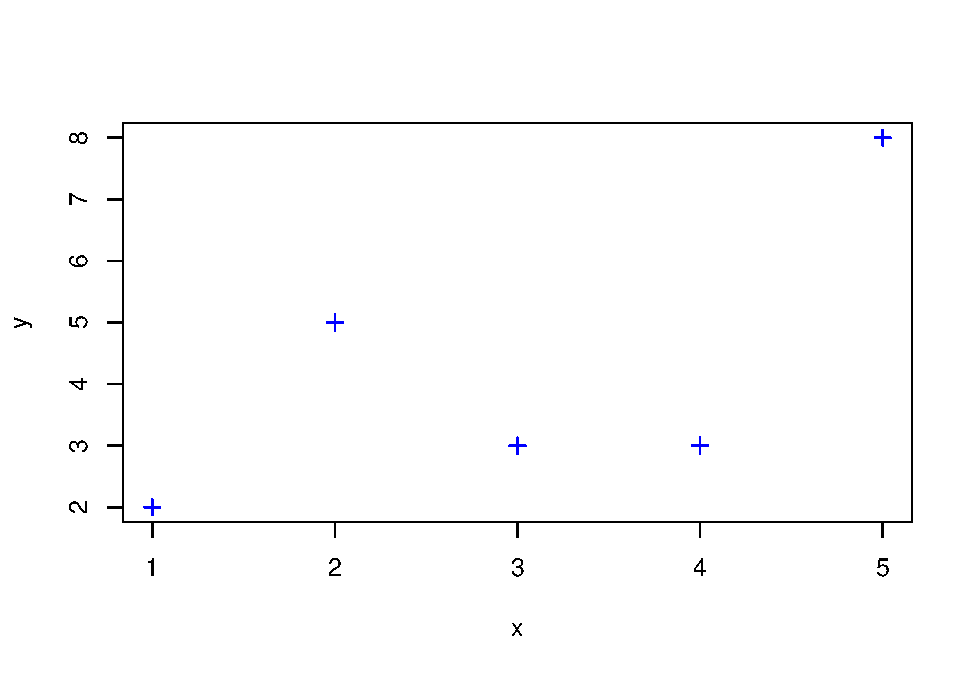
\includegraphics{R-ohjelmoinnin-perusteet_files/figure-latex/unnamed-chunk-149-1.pdf}

\begin{Shaded}
\begin{Highlighting}[]
\NormalTok{value}
\end{Highlighting}
\end{Shaded}

\begin{verbatim}
## NULL
\end{verbatim}

\hypertarget{ifelse}{%
\chapter{Ehtorakenteet}\label{ifelse}}

\protect\hyperlink{functions}{Funktiot} kappaleen funktiot suorittavat aina samat komennot riippumatta syötteestä. Entä jos funktion toiminnassa pitäisi ottaa huomioon erilaisia tapauksia, eli suorittaa tiettyjä komentoja vain joissain tilanteissa? Tätä varten ohjelmointikielissä on ehtorakenteita, eli ns. if/else-rakenteita, jotka ohjaavat ohjelman toimintaa.

Tutustutaan ensin tarkemmin loogisiin operaattoreihin.

\hypertarget{loogiset-operaattorit}{%
\section{Loogiset operaattorit}\label{loogiset-operaattorit}}

Tässä on lyhyt lista loogisista operaattoreista:

\begin{longtable}[]{@{}ll@{}}
\toprule
Operaattori & Toiminto \\
\midrule
\endhead
\textless{} & pienempi kuin \\
\textless= & pienempi tai yhtä suuri kuin \\
\textgreater{} & suurempi kuin \\
\textgreater= & suurempi tai yhtä suuri kuin \\
== & yhtä kuin \\
!= & ei yhtä kuin \\
!a & ei a (negaation) \\
a \textbar{} b & a TAI b alkioittain \\
a \textbar\textbar{} b & a TAI b yksittäisille arvoille \\
a \& b & a JA b alkioittain \\
a \&\& b & a JA b yksittäisille arvoille \\
a \%in\% b & mitkä a:n alkiot ovat myös b:n alkioita \\
\bottomrule
\end{longtable}

Kaikki loogiset operaattorit palauttavat joko arvon \texttt{TRUE}, \texttt{FALSE} tai \texttt{NA}. Vertailuoperaattorien käyttö on jo tullut tutuksi aikaisemmissa kappaleissa, mutta tutustutaan vähän tarkemmin viimeisten rivien operaattoreihin.

\hypertarget{negaatio}{%
\subsubsection{Negaatio}\label{negaatio}}

Looginen negaatio palauttaa loogisen lauseen vastakohdan, eli muuttaa arvon \texttt{TRUE} arvoksi \texttt{FALSE} ja arvon \texttt{FALSE} arvoksi \texttt{TRUE}.

\begin{Shaded}
\begin{Highlighting}[]
\DecValTok{10} \SpecialCharTok{\textgreater{}} \DecValTok{12}
\end{Highlighting}
\end{Shaded}

\begin{verbatim}
## [1] FALSE
\end{verbatim}

\begin{Shaded}
\begin{Highlighting}[]
\SpecialCharTok{!}\NormalTok{(}\DecValTok{10} \SpecialCharTok{\textgreater{}} \DecValTok{12}\NormalTok{)}
\end{Highlighting}
\end{Shaded}

\begin{verbatim}
## [1] TRUE
\end{verbatim}

\begin{Shaded}
\begin{Highlighting}[]
\CommentTok{\# Also works without parentheses}
\SpecialCharTok{!}\DecValTok{10} \SpecialCharTok{\textgreater{}} \DecValTok{12}
\end{Highlighting}
\end{Shaded}

\begin{verbatim}
## [1] TRUE
\end{verbatim}

\begin{Shaded}
\begin{Highlighting}[]
\SpecialCharTok{!}\FunctionTok{is.na}\NormalTok{(}\ConstantTok{NA}\NormalTok{)}
\end{Highlighting}
\end{Shaded}

\begin{verbatim}
## [1] FALSE
\end{verbatim}

\hypertarget{looginen-tai-disjunktio}{%
\subsubsection{Looginen TAI (disjunktio)}\label{looginen-tai-disjunktio}}

Loogiselle TAI operaattorille annetaan kaksi loogista lausetta, ja TAI operaattori palauttaa \texttt{TRUE}, jos vähintään toinen lauseista on \texttt{TRUE}. R:ssä TAI merkitään pystyviivalla \texttt{\textbar{}} tai kahdella pystyviivalla \texttt{\textbar{}\textbar{}}. \texttt{\textbar{}} käy läpi vektoreita alkioittain, \texttt{\textbar{}\textbar{}} vertaa kahta loogista lausetta, ja toista lausetta ei edes ajeta, jos ensimmäinen on \texttt{TRUE} (koska \texttt{\textbar{}\textbar{}} palauttaa \texttt{TRUE} riippumatta toisen lauseen arvosta). Jos tämä tuntui monimutkaiselta, niin riittää muistaa, että ehtorakenteissa kannattaa käyttää muotoa ``\textbar\textbar{}''.

\begin{Shaded}
\begin{Highlighting}[]
\DecValTok{10} \SpecialCharTok{\textgreater{}} \DecValTok{12} \SpecialCharTok{||} \StringTok{"a"} \SpecialCharTok{\textless{}} \StringTok{"b"}
\end{Highlighting}
\end{Shaded}

\begin{verbatim}
## [1] TRUE
\end{verbatim}

\begin{Shaded}
\begin{Highlighting}[]
\DecValTok{2} \SpecialCharTok{\textgreater{}} \DecValTok{1} \SpecialCharTok{||} \DecValTok{4} \SpecialCharTok{\textgreater{}} \DecValTok{2}
\end{Highlighting}
\end{Shaded}

\begin{verbatim}
## [1] TRUE
\end{verbatim}

\begin{Shaded}
\begin{Highlighting}[]
\StringTok{"a"} \SpecialCharTok{\textgreater{}} \StringTok{"c"} \SpecialCharTok{||} \DecValTok{1} \SpecialCharTok{\textgreater{}} \DecValTok{10}
\end{Highlighting}
\end{Shaded}

\begin{verbatim}
## [1] FALSE
\end{verbatim}

\hypertarget{looginen-ja-konjunktio}{%
\subsubsection{Looginen JA (konjunktio)}\label{looginen-ja-konjunktio}}

Loogiselle JA operaattorille annetaan kaksi lausetta. JA palauttaa \texttt{TRUE}, jos kummatkin lauseet ovat \texttt{TRUE}. R:ssä JA-operaattorit ovat \texttt{\&} ja \texttt{\&\&}, jotka käyttäytyvät kuten \texttt{\textbar{}} ja \texttt{\textbar{}\textbar{}}.

\begin{Shaded}
\begin{Highlighting}[]
\DecValTok{10} \SpecialCharTok{\textgreater{}} \DecValTok{12} \SpecialCharTok{\&\&} \StringTok{"a"} \SpecialCharTok{\textless{}} \StringTok{"b"}
\end{Highlighting}
\end{Shaded}

\begin{verbatim}
## [1] FALSE
\end{verbatim}

\begin{Shaded}
\begin{Highlighting}[]
\DecValTok{2} \SpecialCharTok{\textgreater{}} \DecValTok{1} \SpecialCharTok{\&\&} \DecValTok{4} \SpecialCharTok{\textgreater{}} \DecValTok{2}
\end{Highlighting}
\end{Shaded}

\begin{verbatim}
## [1] TRUE
\end{verbatim}

\begin{Shaded}
\begin{Highlighting}[]
\StringTok{"a"} \SpecialCharTok{\textgreater{}} \StringTok{"c"} \SpecialCharTok{\&\&} \DecValTok{1} \SpecialCharTok{\textgreater{}} \DecValTok{10}
\end{Highlighting}
\end{Shaded}

\begin{verbatim}
## [1] FALSE
\end{verbatim}

\hypertarget{osajoukko}{%
\subsubsection{Osajoukko}\label{osajoukko}}

\texttt{\%in\%}-operaattorilla voi tarkistaa, kuuluuko jokin arvo suurempaan joukkoon. Tämä voitaisiin toteuttaa myös usealla TAI-operaattorilla, mutta \texttt{\%in\%} on usein paljon kätevämpi.

\begin{Shaded}
\begin{Highlighting}[]
\NormalTok{dna\_bases }\OtherTok{\textless{}{-}} \FunctionTok{c}\NormalTok{(}\StringTok{"A"}\NormalTok{, }\StringTok{"C"}\NormalTok{, }\StringTok{"G"}\NormalTok{, }\StringTok{"T"}\NormalTok{)}
\NormalTok{rna\_bases }\OtherTok{\textless{}{-}} \FunctionTok{c}\NormalTok{(}\StringTok{"A"}\NormalTok{, }\StringTok{"C"}\NormalTok{, }\StringTok{"G"}\NormalTok{, }\StringTok{"U"}\NormalTok{)}

\StringTok{"T"} \SpecialCharTok{\%in\%}\NormalTok{ dna\_bases}
\end{Highlighting}
\end{Shaded}

\begin{verbatim}
## [1] TRUE
\end{verbatim}

\begin{Shaded}
\begin{Highlighting}[]
\StringTok{"T"} \SpecialCharTok{\%in\%}\NormalTok{ rna\_bases}
\end{Highlighting}
\end{Shaded}

\begin{verbatim}
## [1] FALSE
\end{verbatim}

\begin{Shaded}
\begin{Highlighting}[]
\CommentTok{\# With negation}
\SpecialCharTok{!}\StringTok{"A"} \SpecialCharTok{\%in\%}\NormalTok{ dna\_bases}
\end{Highlighting}
\end{Shaded}

\begin{verbatim}
## [1] FALSE
\end{verbatim}

Operaattoria voi soveltaa myös vektoreihin, jolloin operaattori palauttaa loogisen vektorin, jonka alkio jokainen alkio kertoo, kuuluiko vastaava operaation vasemman puolen alkio operaation oikeaan puoleen.

\begin{Shaded}
\begin{Highlighting}[]
\NormalTok{dna\_bases }\SpecialCharTok{\%in\%}\NormalTok{ rna\_bases}
\end{Highlighting}
\end{Shaded}

\begin{verbatim}
## [1]  TRUE  TRUE  TRUE FALSE
\end{verbatim}

\hypertarget{monimutkaisemmat-lauseet}{%
\subsubsection{Monimutkaisemmat lauseet}\label{monimutkaisemmat-lauseet}}

Operaattoreita voidaan myös yhdistellä monimutkaisemmiksi lauseiksi. Tällöin lauseiden evaluointijärjestys määritetään tarvittaessa suluilla.

\begin{Shaded}
\begin{Highlighting}[]
\NormalTok{dog }\OtherTok{\textless{}{-}} \FunctionTok{list}\NormalTok{(}\AttributeTok{breed =} \StringTok{"golden retriever"}\NormalTok{,}
            \AttributeTok{height =} \DecValTok{45}\NormalTok{,}
            \AttributeTok{weight =} \DecValTok{27}\NormalTok{)}

\NormalTok{dog}\SpecialCharTok{$}\NormalTok{breed }\SpecialCharTok{==} \StringTok{"golden retriever"} \SpecialCharTok{\&\&}\NormalTok{ dog}\SpecialCharTok{$}\NormalTok{weight }\SpecialCharTok{\textless{}} \DecValTok{25} \SpecialCharTok{||}\NormalTok{ dog}\SpecialCharTok{$}\NormalTok{height }\SpecialCharTok{\textless{}} \DecValTok{50}
\end{Highlighting}
\end{Shaded}

\begin{verbatim}
## [1] TRUE
\end{verbatim}

\hypertarget{a-x-b}{%
\subsubsection{a \textless{} x \textless{} b}\label{a-x-b}}

usein tulee vastaan tilanteita, joissa halutaan tarkistaa, onko jokin luku halutulla välillä. Tämä kirjoitetaan matemaatiisesti esim. näin: \(a < x < b\), jossa tarkastetaan, onko \(x\) välillä \((a, b)\). Tämä ei kuitenkaan valitettavasti toimi R:ssä, vaan tarkistus pitää jakaa kahteen osaan:

\begin{Shaded}
\begin{Highlighting}[]
\CommentTok{\# Are x and y between 0 and 1?}
\NormalTok{x }\OtherTok{\textless{}{-}} \DecValTok{3}
\NormalTok{y }\OtherTok{\textless{}{-}} \FloatTok{0.3}
\DecValTok{0} \SpecialCharTok{\textless{}=}\NormalTok{ x }\SpecialCharTok{\&\&}\NormalTok{ x }\SpecialCharTok{\textless{}=} \DecValTok{1}
\end{Highlighting}
\end{Shaded}

\begin{verbatim}
## [1] FALSE
\end{verbatim}

\begin{Shaded}
\begin{Highlighting}[]
\DecValTok{0} \SpecialCharTok{\textless{}=}\NormalTok{ y }\SpecialCharTok{\&\&}\NormalTok{ y }\SpecialCharTok{\textless{}=} \DecValTok{1}
\end{Highlighting}
\end{Shaded}

\begin{verbatim}
## [1] TRUE
\end{verbatim}

\hypertarget{ehtorakenteet}{%
\section{Ehtorakenteet}\label{ehtorakenteet}}

Aloitetaan esimerkistä: tehtävänä on kirjoittaa funktio, jolle annetaan syötteenä potilaan hemoglobiiniarvo. Funktion on tarkoitus hälyttää, jos hemoglobiini laskee alle viitearvojen alarajan 117. Kyseinen funktio voisi näyttää vaikka tältä:

\begin{Shaded}
\begin{Highlighting}[]
\NormalTok{hb\_alert }\OtherTok{\textless{}{-}} \ControlFlowTok{function}\NormalTok{(hb) \{}
  \ControlFlowTok{if}\NormalTok{ (hb }\SpecialCharTok{\textless{}} \DecValTok{117}\NormalTok{) \{}
    \FunctionTok{return}\NormalTok{(}\StringTok{"Hemoglobin is low!"}\NormalTok{)}
\NormalTok{  \}}
\NormalTok{\}}
\end{Highlighting}
\end{Shaded}

Funktiolla on siis yksi argumentti, \texttt{hb} eli hemoglobiiniarvo. Funktion sisällä on if-rakenne. If-rakenteessa on kaksi osaa: ehto, ja rakenteen sisäinen koodi. Rakenteen sisäinen koodi ajetaan vain, jos ehto täyttyy. Ehto merkitään if-komennon jälkeen sulkeisiin, ja rakenteen sisäinen koodi kirjoitetaan sulkeiden jälkeen aaltosulkeiden sisään. (Jos aaltosulkeiden sisään tulisi vain yksi rivi koodia, aaltoasulkeet voi jättää pois, mutta näissä esimerkeissä käytetään aina aaltoasulkeita).

Kokeillaan, miten funktio toimii eri hemoglobiiniarvoilla:

\begin{Shaded}
\begin{Highlighting}[]
\CommentTok{\# Nothing happens}
\FunctionTok{hb\_alert}\NormalTok{(}\DecValTok{130}\NormalTok{)}
\CommentTok{\# returns alert}
\FunctionTok{hb\_alert}\NormalTok{(}\DecValTok{110}\NormalTok{)}
\end{Highlighting}
\end{Shaded}

\begin{verbatim}
## [1] "Hemoglobin is low!"
\end{verbatim}

Funktio siis toimii oletetusti, eli se hälyttää vain, jos hemoglobiinitaso on alle 117. Käyttäjän kannalta olisi kuitenkin kätevää saada jonkinlainen palaute myös silloin, kun hemoglobiinitaso on tarpeeksi korkea. Tätä varten voidaan käyttää else-komentoa:

\begin{Shaded}
\begin{Highlighting}[]
\NormalTok{hb\_alert }\OtherTok{\textless{}{-}} \ControlFlowTok{function}\NormalTok{(hb) \{}
  \ControlFlowTok{if}\NormalTok{ (hb }\SpecialCharTok{\textless{}} \DecValTok{117}\NormalTok{) \{}
    \FunctionTok{return}\NormalTok{(}\StringTok{"Hemoglobin is low!"}\NormalTok{)}
\NormalTok{  \} }\ControlFlowTok{else}\NormalTok{ \{}
    \FunctionTok{return}\NormalTok{(}\StringTok{"Hemoglobin OK"}\NormalTok{)}
\NormalTok{  \}}
\NormalTok{\}}

\FunctionTok{hb\_alert}\NormalTok{(}\DecValTok{130}\NormalTok{)}
\end{Highlighting}
\end{Shaded}

\begin{verbatim}
## [1] "Hemoglobin OK"
\end{verbatim}

Else-komennon jälkeinen koodi siis ajetaan, jos ehto \texttt{hb\ \textless{}\ 117} ei täyty.

Tällä hetkellä funktiomme toimii vain naispotilaille, sillä miehillä hemoglobiiniarvojen alaraja on 134. Lisätään siis funktioomme argumentti \texttt{sex} sukupuolta varten ja muokataan funktion toimintaa niin, että se osaa ottaa huomioon sukupuolen. Nyt if-rakenteen ehdosta tulee jo hieman monimutkaisempi:

\begin{Shaded}
\begin{Highlighting}[]
\NormalTok{hb\_alert }\OtherTok{\textless{}{-}} \ControlFlowTok{function}\NormalTok{(hb, sex) \{}
  \ControlFlowTok{if}\NormalTok{ (sex }\SpecialCharTok{==} \StringTok{"female"} \SpecialCharTok{\&\&}\NormalTok{ hb }\SpecialCharTok{\textless{}} \DecValTok{117} \SpecialCharTok{||}\NormalTok{ sex }\SpecialCharTok{==} \StringTok{"male"} \SpecialCharTok{\&\&}\NormalTok{ hb }\SpecialCharTok{\textless{}} \DecValTok{134}\NormalTok{) \{}
    \FunctionTok{return}\NormalTok{(}\StringTok{"Hemoglobin is low!"}\NormalTok{)}
\NormalTok{  \} }\ControlFlowTok{else}\NormalTok{ \{}
    \FunctionTok{return}\NormalTok{(}\StringTok{"Hemoglobin OK"}\NormalTok{)}
\NormalTok{  \}}
\NormalTok{\}}

\FunctionTok{hb\_alert}\NormalTok{(}\AttributeTok{hb =} \DecValTok{120}\NormalTok{, }\AttributeTok{sex =} \StringTok{"female"}\NormalTok{)}
\end{Highlighting}
\end{Shaded}

\begin{verbatim}
## [1] "Hemoglobin OK"
\end{verbatim}

\begin{Shaded}
\begin{Highlighting}[]
\FunctionTok{hb\_alert}\NormalTok{(}\AttributeTok{hb =} \DecValTok{120}\NormalTok{, }\AttributeTok{sex =} \StringTok{"male"}\NormalTok{)}
\end{Highlighting}
\end{Shaded}

\begin{verbatim}
## [1] "Hemoglobin is low!"
\end{verbatim}

Entä jos haluaisimme tulostaa eri varoituksen mies- ja naispotilaille? Tähän tarvitaan ``else if''-rakennetta:

\begin{Shaded}
\begin{Highlighting}[]
\NormalTok{hb\_alert }\OtherTok{\textless{}{-}} \ControlFlowTok{function}\NormalTok{(hb, sex) \{}
  \ControlFlowTok{if}\NormalTok{ (sex }\SpecialCharTok{==} \StringTok{"female"} \SpecialCharTok{\&\&}\NormalTok{ hb }\SpecialCharTok{\textless{}} \DecValTok{117}\NormalTok{) \{}
    \FunctionTok{return}\NormalTok{(}\StringTok{"Hemoglobin is low for a female!"}\NormalTok{)}
\NormalTok{  \} }\ControlFlowTok{else} \ControlFlowTok{if}\NormalTok{ (sex }\SpecialCharTok{==} \StringTok{"male"} \SpecialCharTok{\&\&}\NormalTok{ hb }\SpecialCharTok{\textless{}} \DecValTok{134}\NormalTok{) \{}
    \FunctionTok{return}\NormalTok{(}\StringTok{"Hemoglobin is low for a male!"}\NormalTok{)}
\NormalTok{  \} }\ControlFlowTok{else}\NormalTok{ \{}
    \FunctionTok{return}\NormalTok{(}\StringTok{"Hemoglobin OK"}\NormalTok{)}
\NormalTok{  \}}
\NormalTok{\}}

\FunctionTok{hb\_alert}\NormalTok{(}\AttributeTok{hb =} \DecValTok{110}\NormalTok{, }\AttributeTok{sex =} \StringTok{"female"}\NormalTok{)}
\end{Highlighting}
\end{Shaded}

\begin{verbatim}
## [1] "Hemoglobin is low for a female!"
\end{verbatim}

\begin{Shaded}
\begin{Highlighting}[]
\FunctionTok{hb\_alert}\NormalTok{(}\AttributeTok{hb =} \DecValTok{120}\NormalTok{, }\AttributeTok{sex =} \StringTok{"male"}\NormalTok{)}
\end{Highlighting}
\end{Shaded}

\begin{verbatim}
## [1] "Hemoglobin is low for a male!"
\end{verbatim}

Nyt funktio tarkistaa ensin, onko potilas nainen ja onko hänen hemoglobiininsa alle 117. Jos ei, siirrytään eteenpäin ja tarkistetaan, onko potilas mies ja onko hänen hemoglobiininsa alle 130. Jos ei, siirrytään viimeiseen kohtaan, ja tulostetaan ``Hemoglobin ok''.

Else-if rakenteita voi olla rajoittamaton määrä ensimmäisen if-rakenteen jälkeen. Lisätään funktioon hälytys kriittisestä hemoglobiinin määrästä (hb \textless{} 50) riippumatta sukupuolesta:

\begin{Shaded}
\begin{Highlighting}[]
\NormalTok{hb\_alert }\OtherTok{\textless{}{-}} \ControlFlowTok{function}\NormalTok{(hb, sex) \{}
  \ControlFlowTok{if}\NormalTok{ (sex }\SpecialCharTok{==} \StringTok{"female"} \SpecialCharTok{\&\&}\NormalTok{ hb }\SpecialCharTok{\textless{}} \DecValTok{117}\NormalTok{) \{}
    \FunctionTok{return}\NormalTok{(}\StringTok{"Hemoglobin is low for a female!"}\NormalTok{)}
\NormalTok{  \} }\ControlFlowTok{else} \ControlFlowTok{if}\NormalTok{ (sex }\SpecialCharTok{==} \StringTok{"male"} \SpecialCharTok{\&\&}\NormalTok{ hb }\SpecialCharTok{\textless{}} \DecValTok{134}\NormalTok{) \{}
    \FunctionTok{return}\NormalTok{(}\StringTok{"Hemoglobin is low for a male!"}\NormalTok{)}
\NormalTok{  \} }\ControlFlowTok{else} \ControlFlowTok{if}\NormalTok{ (hb }\SpecialCharTok{\textless{}} \DecValTok{50}\NormalTok{) \{}
    \FunctionTok{return}\NormalTok{(}\StringTok{"Hemoglobin is critical"}\NormalTok{)}
\NormalTok{  \} }\ControlFlowTok{else}\NormalTok{ \{}
    \FunctionTok{return}\NormalTok{(}\StringTok{"Hemoglobin OK"}\NormalTok{)}
\NormalTok{  \}}
\NormalTok{\}}

\FunctionTok{hb\_alert}\NormalTok{(}\AttributeTok{hb =} \DecValTok{32}\NormalTok{, }\AttributeTok{sex =} \StringTok{"female"}\NormalTok{)}
\end{Highlighting}
\end{Shaded}

\begin{verbatim}
## [1] "Hemoglobin is low for a female!"
\end{verbatim}

Kuten huomataan, yllä oleva koodi ei toimikaan, kuten piti. Näin alhaisella hemoglobiinilla pitäisi tulla varoitus kriittisestä tilasta. Koodi suoritus ei kuitenkaan ikinä etene kriittisen tilan varoitukseen asti, sillä ensimmäinen ehto täyttyy. Korjataan tilanne siirtämällä kriittisen tilan ehto ensimmäiseksi:

\begin{Shaded}
\begin{Highlighting}[]
\NormalTok{hb\_alert }\OtherTok{\textless{}{-}} \ControlFlowTok{function}\NormalTok{(hb, sex) \{}
  \ControlFlowTok{if}\NormalTok{ (hb }\SpecialCharTok{\textless{}} \DecValTok{50}\NormalTok{) \{}
    \FunctionTok{return}\NormalTok{(}\StringTok{"Hemoglobin is critical"}\NormalTok{)}
\NormalTok{  \} }\ControlFlowTok{else} \ControlFlowTok{if}\NormalTok{ (sex }\SpecialCharTok{==} \StringTok{"male"} \SpecialCharTok{\&\&}\NormalTok{ hb }\SpecialCharTok{\textless{}} \DecValTok{134}\NormalTok{) \{}
    \FunctionTok{return}\NormalTok{(}\StringTok{"Hemoglobin is low for a male!"}\NormalTok{)}
\NormalTok{  \} }\ControlFlowTok{else} \ControlFlowTok{if}\NormalTok{ (sex }\SpecialCharTok{==} \StringTok{"female"} \SpecialCharTok{\&\&}\NormalTok{ hb }\SpecialCharTok{\textless{}} \DecValTok{117}\NormalTok{) \{}
    \FunctionTok{return}\NormalTok{(}\StringTok{"Hemoglobin is low for a female!"}\NormalTok{)}
\NormalTok{  \} }\ControlFlowTok{else}\NormalTok{ \{}
    \FunctionTok{return}\NormalTok{(}\StringTok{"Hemoglobin OK"}\NormalTok{)}
\NormalTok{  \}}
\NormalTok{\}}

\FunctionTok{hb\_alert}\NormalTok{(}\AttributeTok{hb =} \DecValTok{32}\NormalTok{, }\AttributeTok{sex =} \StringTok{"female"}\NormalTok{)}
\end{Highlighting}
\end{Shaded}

\begin{verbatim}
## [1] "Hemoglobin is critical"
\end{verbatim}

\begin{Shaded}
\begin{Highlighting}[]
\FunctionTok{hb\_alert}\NormalTok{(}\AttributeTok{hb =} \DecValTok{120}\NormalTok{, }\AttributeTok{sex =} \StringTok{"female"}\NormalTok{)}
\end{Highlighting}
\end{Shaded}

\begin{verbatim}
## [1] "Hemoglobin OK"
\end{verbatim}

\begin{Shaded}
\begin{Highlighting}[]
\FunctionTok{hb\_alert}\NormalTok{(}\AttributeTok{hb =} \DecValTok{120}\NormalTok{, }\AttributeTok{sex =} \StringTok{"male"}\NormalTok{)}
\end{Highlighting}
\end{Shaded}

\begin{verbatim}
## [1] "Hemoglobin is low for a male!"
\end{verbatim}

Nyt funktio toimii haluamallamme tavalla!

Funktioissa voi myös olla useampi ehtorakenne. Ehtorakenteita käytetään usein tarkistamaan argumenttien arvoja. Lisätään ehtorakenteet argumenttien tarkistamiseksi:

\begin{Shaded}
\begin{Highlighting}[]
\NormalTok{hb\_alert }\OtherTok{\textless{}{-}} \ControlFlowTok{function}\NormalTok{(hb, sex) \{}
  \CommentTok{\# Hemoglobin should be numeric and positive}
  \ControlFlowTok{if}\NormalTok{ (}\SpecialCharTok{!}\FunctionTok{is.numeric}\NormalTok{(hb) }\SpecialCharTok{||}\NormalTok{ hb }\SpecialCharTok{\textless{}} \DecValTok{0}\NormalTok{) \{}
    \FunctionTok{return}\NormalTok{(}\StringTok{"Hemoglobin should be numeric and positive"}\NormalTok{)}
\NormalTok{  \}}
  \ControlFlowTok{if}\NormalTok{ (}\SpecialCharTok{!}\NormalTok{sex }\SpecialCharTok{\%in\%} \FunctionTok{c}\NormalTok{(}\StringTok{"female"}\NormalTok{, }\StringTok{"male"}\NormalTok{)) \{}
    \FunctionTok{return}\NormalTok{(}\StringTok{"This function can only deal with binary sex: female or male"}\NormalTok{)}
\NormalTok{  \}}
  
  \ControlFlowTok{if}\NormalTok{ (hb }\SpecialCharTok{\textless{}} \DecValTok{50}\NormalTok{) \{}
    \FunctionTok{return}\NormalTok{(}\StringTok{"Hemoglobin is critical"}\NormalTok{)}
\NormalTok{  \} }\ControlFlowTok{else} \ControlFlowTok{if}\NormalTok{ (sex }\SpecialCharTok{==} \StringTok{"male"} \SpecialCharTok{\&\&}\NormalTok{ hb }\SpecialCharTok{\textless{}} \DecValTok{134}\NormalTok{) \{}
    \FunctionTok{return}\NormalTok{(}\StringTok{"Hemoglobin is low for a male!"}\NormalTok{)}
\NormalTok{  \} }\ControlFlowTok{else} \ControlFlowTok{if}\NormalTok{ (sex }\SpecialCharTok{==} \StringTok{"female"} \SpecialCharTok{\&\&}\NormalTok{ hb }\SpecialCharTok{\textless{}} \DecValTok{117}\NormalTok{) \{}
    \FunctionTok{return}\NormalTok{(}\StringTok{"Hemoglobin is low for a female!"}\NormalTok{)}
\NormalTok{  \} }\ControlFlowTok{else}\NormalTok{ \{}
    \FunctionTok{return}\NormalTok{(}\StringTok{"Hemoglobin OK"}\NormalTok{)}
\NormalTok{  \}}
\NormalTok{\}}

\FunctionTok{hb\_alert}\NormalTok{(}\AttributeTok{hb =} \StringTok{"120"}\NormalTok{, }\AttributeTok{sex =} \StringTok{"female"}\NormalTok{)}
\end{Highlighting}
\end{Shaded}

\begin{verbatim}
## [1] "Hemoglobin should be numeric and positive"
\end{verbatim}

\begin{Shaded}
\begin{Highlighting}[]
\FunctionTok{hb\_alert}\NormalTok{(}\AttributeTok{hb =} \DecValTok{120}\NormalTok{, }\AttributeTok{sex =} \StringTok{"FEMALE"}\NormalTok{)}
\end{Highlighting}
\end{Shaded}

\begin{verbatim}
## [1] "This function can only deal with binary sex: female or male"
\end{verbatim}

\hypertarget{alkioiden-poimiminen-vektorista-tietyn-ehdon-perusteella}{%
\section{Alkioiden poimiminen vektorista tietyn ehdon perusteella}\label{alkioiden-poimiminen-vektorista-tietyn-ehdon-perusteella}}

Seuraava tilanne on melko tyypillinen: on käytävä läpi vektorin arvot, ja säilytettävä niistä ne, jotka täyttivät tietyn ehdon. Tätä ongelmaa voi lähestyä esimerkiksi seuraavalla tavalla:

\begin{itemize}
\tightlist
\item
  Luo apufunktio, joka ottaa syötteeksi yhden arvon, ja tarkistaa täyttyykö ehto. Tämän funktion tulee palauttaa \texttt{TRUE}, jos ehto täyttyy ja \texttt{FALSE}, jos ehto ei täyty.
\item
  Käytä funktiota \texttt{Vectorize}, jolla voit muuttaa funktiosi vektoroiduksi funktioksi. Vektorointi tarkoittaa tässä yhteydessä sitä, että yhden alkion sijaan vektoroitua funktiota voidaankin kutsua vektoriargumentilla, ja jokaiselle argumentin alkiolle suoritetaan alkuperäisen funktion määrittelemä operaatio.
\item
  Käytä vektoroitua apufunktiota vektorin indeksointiin.
\end{itemize}

Tässä on esimerkki, jossa käydään läpi vektori DNA:n emäksiä, joista poimitaan vain sytosiinit ja guaniinit.

\begin{Shaded}
\begin{Highlighting}[]
\CommentTok{\# Helper function}
\NormalTok{is\_cg }\OtherTok{\textless{}{-}} \ControlFlowTok{function}\NormalTok{(base) \{}
  \ControlFlowTok{if}\NormalTok{ (base }\SpecialCharTok{\%in\%} \FunctionTok{c}\NormalTok{(}\StringTok{"C"}\NormalTok{, }\StringTok{"G"}\NormalTok{)) \{}
    \FunctionTok{return}\NormalTok{(}\ConstantTok{TRUE}\NormalTok{)}
\NormalTok{  \} }\ControlFlowTok{else}\NormalTok{ \{}
    \FunctionTok{return}\NormalTok{(}\ConstantTok{FALSE}\NormalTok{)}
\NormalTok{  \}}
\NormalTok{\}}

\CommentTok{\# Vectorize}
\NormalTok{is\_cg\_vector }\OtherTok{\textless{}{-}} \FunctionTok{Vectorize}\NormalTok{(is\_cg)}

\CommentTok{\# Main function}
\NormalTok{pick\_cg }\OtherTok{\textless{}{-}} \ControlFlowTok{function}\NormalTok{(bases) \{}
\NormalTok{  only\_cg }\OtherTok{\textless{}{-}}\NormalTok{ bases[}\FunctionTok{is\_cg\_vector}\NormalTok{(bases)]}
  \FunctionTok{return}\NormalTok{(only\_cg)}
\NormalTok{\}}

\CommentTok{\# }\AlertTok{NOTE}\CommentTok{: this only checks the first value of the vector}
\NormalTok{my\_bases }\OtherTok{\textless{}{-}} \FunctionTok{c}\NormalTok{(}\StringTok{"A"}\NormalTok{, }\StringTok{"C"}\NormalTok{, }\StringTok{"C"}\NormalTok{, }\StringTok{"T"}\NormalTok{, }\StringTok{"G"}\NormalTok{, }\StringTok{"T"}\NormalTok{)}
\FunctionTok{is\_cg}\NormalTok{(my\_bases)}
\end{Highlighting}
\end{Shaded}

\begin{verbatim}
## Warning in if (base %in% c("C", "G")) {: the condition has length > 1 and only
## the first element will be used
\end{verbatim}

\begin{verbatim}
## [1] FALSE
\end{verbatim}

\begin{Shaded}
\begin{Highlighting}[]
\CommentTok{\# This works as expected}
\FunctionTok{is\_cg\_vector}\NormalTok{(my\_bases)}
\end{Highlighting}
\end{Shaded}

\begin{verbatim}
##     A     C     C     T     G     T 
## FALSE  TRUE  TRUE FALSE  TRUE FALSE
\end{verbatim}

\begin{Shaded}
\begin{Highlighting}[]
\CommentTok{\# Pick only C and G}
\FunctionTok{pick\_cg}\NormalTok{(my\_bases)}
\end{Highlighting}
\end{Shaded}

\begin{verbatim}
## [1] "C" "C" "G"
\end{verbatim}

\hypertarget{loops}{%
\chapter{Toistorakenteet (loops)}\label{loops}}

Toistorakenne toistaa annettua koodia. Toistorakenteet ovat ehtorakenteiden ohella ohjelmoinnin perusrakennuspalikoita. Tässä osiossa tutustutaan kahteen yleisimpään tapaukseen eli for ja while -silmukoihin. Mukana on myös maininta silmukoiden korvaamisesta R:n apply-funktioilla. Lopusta löytyy lisäksi vinkkejä tämän viikon tehtäviin.

Lisäksi tällä viikolla puhutaan R-paketeista.

\hypertarget{for-silmukka}{%
\section{For-silmukka}\label{for-silmukka}}

For-silmukka toistaa koodia ennalta määrättyjen iteraatioiden verran. For-silmukalla voi esimerkiksi käydä läpi data framen tai matriisin sarakkeita tai rivejä, tai vektorin arvoja. For-silmukka iteroi aina jonkin järjestetyn rakenteen yli, esimerkiksi vektorin. For-silmukalle annetaan tyypillisesti vektori arvoja, ja ns. iteraatiomuuttuja, johon tallennetaan vuorotellen yksi alkio annetusta vektorista. Käytännössä tämä näyttää tältä:

\begin{Shaded}
\begin{Highlighting}[]
\ControlFlowTok{for}\NormalTok{ (i }\ControlFlowTok{in} \FunctionTok{seq}\NormalTok{(}\DecValTok{3}\NormalTok{, }\DecValTok{7}\NormalTok{)) \{}
  \FunctionTok{print}\NormalTok{(i)}
\NormalTok{\}}
\end{Highlighting}
\end{Shaded}

for-silmukassa määritetään siis ensin iteraatiomuuttuja eli \texttt{i} ja sen saamat arvot eli \texttt{seq(3,\ 7)} komennolla \texttt{in}. Sen jälkeen hakasulkeiden sisältämä koodi toistetaan jokaiselle \texttt{i}:n arvolle. Tässä tapauksessa yksinkertaisesti tulostetaan muuttujan \texttt{i} arvo. Huomaa, että for-silmukan \texttt{ìn} ei ole sama asia kuin looginen operaattori \texttt{\%in\%}.

Usein halutaan kuitenkin käydä läpi jonkin vektorin tai matriisin arvoja. Alla oleva koodi laskee matriisin X rivien summan (tähän voisi myös käyttää valmista funktiota \texttt{rowSums()}). Aluksi alustetaan tyhjä vektori, johon rivien summat tallennetaan. Sen jälkeen käydään läpi matriisin rivit ja tallennetaan rivin summa alussa alustettuun vektoriin.

\begin{Shaded}
\begin{Highlighting}[]
\CommentTok{\# Create matrix X}
\NormalTok{X }\OtherTok{\textless{}{-}} \FunctionTok{matrix}\NormalTok{(}\DecValTok{1}\SpecialCharTok{:}\DecValTok{12}\NormalTok{, }\AttributeTok{nrow =} \DecValTok{4}\NormalTok{)}
\NormalTok{X}

\CommentTok{\# Initialize vector for row sums}
\NormalTok{row\_sums }\OtherTok{\textless{}{-}} \FunctionTok{rep}\NormalTok{(}\DecValTok{0}\NormalTok{, }\FunctionTok{nrow}\NormalTok{(X))}
\CommentTok{\# Iterate over rows of X}
\ControlFlowTok{for}\NormalTok{ (i }\ControlFlowTok{in} \FunctionTok{seq}\NormalTok{(}\DecValTok{1}\NormalTok{, }\FunctionTok{nrow}\NormalTok{(X))) \{}
  \CommentTok{\# Assign sum of the current row to the vector}
\NormalTok{  row\_sums[i] }\OtherTok{\textless{}{-}} \FunctionTok{sum}\NormalTok{(X[i, ])}
\NormalTok{\}}

\CommentTok{\# Compare results with the result from base R function}
\NormalTok{row\_sums}
\FunctionTok{rowSums}\NormalTok{(X)}
\end{Highlighting}
\end{Shaded}

For-silmukalla voi myös toteuttaa viime kerralla tehdyn funktion, joka poimii DNA:n emäksistä vain sytosiinit ja guaniinit. Tällä kertaa apufunktiota \texttt{is\_cg()} ei tarvitse vektorisoida, koska for-silmukka käy läpi kaikki emäkset. Tämä silmukka voidaan toteuttaa kahdella tavalla. Ensimmäinen tapa on käyttää iteraatiomuuttujana i:tä, joka käy läpi iteraation ykkösestä emäsvektroin pituuteen:

\begin{Shaded}
\begin{Highlighting}[]
\CommentTok{\# Helper function}
\NormalTok{is\_cg }\OtherTok{\textless{}{-}} \ControlFlowTok{function}\NormalTok{(base) \{}
  \ControlFlowTok{if}\NormalTok{ (base }\SpecialCharTok{\%in\%} \FunctionTok{c}\NormalTok{(}\StringTok{"C"}\NormalTok{, }\StringTok{"G"}\NormalTok{)) \{}
    \FunctionTok{return}\NormalTok{(}\ConstantTok{TRUE}\NormalTok{)}
\NormalTok{  \} }\ControlFlowTok{else}\NormalTok{ \{}
    \FunctionTok{return}\NormalTok{(}\ConstantTok{FALSE}\NormalTok{)}
\NormalTok{  \}}
\NormalTok{\}}

\CommentTok{\# Main function}
\NormalTok{pick\_cg1 }\OtherTok{\textless{}{-}} \ControlFlowTok{function}\NormalTok{(bases) \{}
  \CommentTok{\# Initialize empty vector}
\NormalTok{  only\_cg }\OtherTok{\textless{}{-}} \FunctionTok{c}\NormalTok{()}
  \ControlFlowTok{for}\NormalTok{ (i }\ControlFlowTok{in} \FunctionTok{seq}\NormalTok{(}\DecValTok{1}\NormalTok{, }\FunctionTok{length}\NormalTok{(bases))) \{}
    \CommentTok{\# If the current base is C or G, add it to only\_cg}
    \ControlFlowTok{if}\NormalTok{ (}\FunctionTok{is\_cg}\NormalTok{(bases[i])) \{}
\NormalTok{      only\_cg }\OtherTok{\textless{}{-}} \FunctionTok{c}\NormalTok{(only\_cg, bases[i])}
\NormalTok{    \}}
\NormalTok{  \}}
  
  \FunctionTok{return}\NormalTok{(only\_cg)}
\NormalTok{\}}

\NormalTok{my\_bases }\OtherTok{\textless{}{-}} \FunctionTok{c}\NormalTok{(}\StringTok{"A"}\NormalTok{, }\StringTok{"C"}\NormalTok{, }\StringTok{"C"}\NormalTok{, }\StringTok{"T"}\NormalTok{, }\StringTok{"G"}\NormalTok{, }\StringTok{"T"}\NormalTok{)}
\FunctionTok{pick\_cg1}\NormalTok{(my\_bases)}
\end{Highlighting}
\end{Shaded}

Toinen vaihtoehto on iteroida suoraan vektorin bases yli, jolloin iteraatiomuuttujaan tallentuu suoraan kyseinen emäs:

\begin{Shaded}
\begin{Highlighting}[]
\NormalTok{pick\_cg2 }\OtherTok{\textless{}{-}} \ControlFlowTok{function}\NormalTok{(bases) \{}
  \CommentTok{\# Initialize empty vector}
\NormalTok{  only\_cg }\OtherTok{\textless{}{-}} \FunctionTok{c}\NormalTok{()}
  \ControlFlowTok{for}\NormalTok{ (base }\ControlFlowTok{in}\NormalTok{ bases) \{}
    \CommentTok{\# If the current base is C or G, add it to only\_cg}
    \ControlFlowTok{if}\NormalTok{ (}\FunctionTok{is\_cg}\NormalTok{(base)) \{}
\NormalTok{      only\_cg }\OtherTok{\textless{}{-}} \FunctionTok{c}\NormalTok{(only\_cg, base)}
\NormalTok{    \}}
\NormalTok{  \}}
  
  \FunctionTok{return}\NormalTok{(only\_cg)}
\NormalTok{\}}

\NormalTok{my\_bases }\OtherTok{\textless{}{-}} \FunctionTok{c}\NormalTok{(}\StringTok{"A"}\NormalTok{, }\StringTok{"C"}\NormalTok{, }\StringTok{"C"}\NormalTok{, }\StringTok{"T"}\NormalTok{, }\StringTok{"G"}\NormalTok{, }\StringTok{"T"}\NormalTok{)}
\FunctionTok{pick\_cg2}\NormalTok{(my\_bases)}
\end{Highlighting}
\end{Shaded}

Iteraatiomuuttujan voi siis nimetä haluamallaan tavalla, sen ei aina tarvitse olla i. Jos kuitenkin iteraatiomuuttujaan tallennetaan vain yksi luku, suosittelen vahvasti käyttämään i:tä. Tämä on hyvin vakiintunut tapa ohjelmointikielestä ja ohjelmoijasta riippumatta, vaikka muutoin muuttujien nimeämiseen on erilaisia koulukuntia riippuen ohjelmoijan taustasta. Jos taas iteroidaan vektorin nimeltä bases yli, on luonnollinen valinta iteraatiomuuttujan nimeksi base.


\includegraphics{files/08-functions/naming.jpg}

\hypertarget{while-slimukat}{%
\section{While-slimukat}\label{while-slimukat}}

While-silmukkaa käytetään, kun iteraatioiden määrä ei ole ennalta tiedossa, vaan while-silmukkaa toistetaan niin kauan, kuin tietty ehto on voimassa. Hyvä esimerkki while-silmukasta on proteiinisynteesi (yksinkertaistettuna): alla oleva funktio käy läpi RNA-molekyylin kodoneita, kunnes löytää aloituskodonin AUG. Sen jälkeen funktio rakentaa aminohappoketjua kodonien perusteella, kunnes vastaan tulee jokin lopetuskodoneista. Oikean proteiinin löytämiseen käytetään Biostrings-paketista löytyvää geneettistä koodia, joka on nimetty vektori, jossa on kodoneita vastaavien aminohappojen kirjainlyhenne, tai lopetuskodonien tapauksessa merkki "*":

\begin{Shaded}
\begin{Highlighting}[]
\NormalTok{rna\_code }\OtherTok{\textless{}{-}}\NormalTok{ Biostrings}\SpecialCharTok{::}\NormalTok{RNA\_GENETIC\_CODE}
\NormalTok{rna\_code}
\end{Highlighting}
\end{Shaded}

\begin{Shaded}
\begin{Highlighting}[]
\NormalTok{prot\_synth }\OtherTok{\textless{}{-}} \ControlFlowTok{function}\NormalTok{(codons) \{}
  \CommentTok{\# Initialize iterable as the first codon}
\NormalTok{  i }\OtherTok{\textless{}{-}} \DecValTok{1}
  \CommentTok{\# Initialize empty amino acid chain}
\NormalTok{  protein }\OtherTok{\textless{}{-}} \FunctionTok{c}\NormalTok{()}
  \CommentTok{\# Find starting codon}
  \ControlFlowTok{while}\NormalTok{ (codons[i] }\SpecialCharTok{!=} \StringTok{"AUG"}\NormalTok{) \{}
\NormalTok{    i }\OtherTok{\textless{}{-}}\NormalTok{ i }\SpecialCharTok{+} \DecValTok{1}
\NormalTok{  \}}
  \CommentTok{\# After starting codon, build protein until one of the stop codons is met}
  \ControlFlowTok{while}\NormalTok{ (rna\_code[codons[i]] }\SpecialCharTok{!=} \StringTok{"*"}\NormalTok{) \{}
\NormalTok{    protein }\OtherTok{\textless{}{-}} \FunctionTok{c}\NormalTok{(protein, rna\_code[codons[i]])}
\NormalTok{    i }\OtherTok{\textless{}{-}}\NormalTok{ i }\SpecialCharTok{+} \DecValTok{1}
\NormalTok{  \}}
  \FunctionTok{return}\NormalTok{(protein)}
\NormalTok{\}}

\FunctionTok{prot\_synth}\NormalTok{(}\AttributeTok{codons =} \FunctionTok{c}\NormalTok{(}\StringTok{"UUG"}\NormalTok{, }\StringTok{"GAA"}\NormalTok{, }\StringTok{"AUG"}\NormalTok{, }\StringTok{"UGU"}\NormalTok{, }\StringTok{"AGU"}\NormalTok{, }\StringTok{"AGA"}\NormalTok{, }\StringTok{"UCG"}\NormalTok{, }\StringTok{"UCG"}\NormalTok{, }\StringTok{"UGA"}\NormalTok{, }\StringTok{"GCA"}\NormalTok{))}
\end{Highlighting}
\end{Shaded}

While-silmukalle annetaan siis ensin ehto, joka tarkistetaan ennen jokaista iteraatiota. Jos ehto täyttyy, suoritetaan yksi iteraatio, ja tarkistetaan ehto uudestaan. HUOM: while-silmukkaa koodatessa tulee huolehtia siitä, että silmukan ehdon on mahdollista olla lopulta epätosi, muuten silmukka saattaa jäädä pyörimään ikuisesti!

Käytännössä kaikki for-silmukat voisi korvata while-silmukoilla, mutta for-silmukoiden käyttö on kätevämpää, sillä niissä iteraatiomuuttujaa ei tarvitse kasvattaa erikseen.

\begin{Shaded}
\begin{Highlighting}[]
\CommentTok{\# A simple for loop}
\ControlFlowTok{for}\NormalTok{ (i }\ControlFlowTok{in} \FunctionTok{seq}\NormalTok{(}\DecValTok{1}\NormalTok{, }\DecValTok{4}\NormalTok{)) \{}
  \FunctionTok{print}\NormalTok{(i }\SpecialCharTok{*} \DecValTok{2}\NormalTok{)}
\NormalTok{\}}

\CommentTok{\# The same as above}
\NormalTok{i }\OtherTok{\textless{}{-}} \DecValTok{1}
\ControlFlowTok{while}\NormalTok{ (i }\SpecialCharTok{\textless{}=} \DecValTok{4}\NormalTok{) \{}
  \FunctionTok{print}\NormalTok{(i }\SpecialCharTok{*} \DecValTok{2}\NormalTok{)}
\NormalTok{  i }\OtherTok{\textless{}{-}}\NormalTok{ i }\SpecialCharTok{+} \DecValTok{1}
\NormalTok{\}}
\end{Highlighting}
\end{Shaded}

\hypertarget{sisuxe4kkuxe4iset-silmukat-nested-loops}{%
\section{Sisäkkäiset silmukat (nested loops)}\label{sisuxe4kkuxe4iset-silmukat-nested-loops}}

Silmukoita voi myös olla useampi sisäkkäin. Alla olevassa esimerkissä on taulukko tutkimuksesta, jossa on mitattu eri eliöiden \(\beta\)- globiinigeenin ensimmäisen eksonin samankaltaisuutta. Pienempi luku tarkoittaa enemmän samankaltaista geeniä.

\begin{tabular}{l|r|r|r|r|r|r|r}
\hline
  & Human & Goat & Opossum & Lemur & Mouse & Rabbit & Gorilla\\
\hline
Human & 0.0 & 4.7 & 4.6 & 2.7 & 3.2 & 3.2 & 1.6\\
\hline
Goat & 4.7 & 0.0 & 7.2 & 5.9 & 7.8 & 3.7 & 5.5\\
\hline
Opossum & 4.6 & 7.2 & 0.0 & 5.3 & 5.3 & 6.3 & 5.7\\
\hline
Lemur & 2.7 & 5.9 & 5.3 & 0.0 & 4.3 & 2.7 & 3.2\\
\hline
Mouse & 3.2 & 7.8 & 5.3 & 4.3 & 0.0 & 6.0 & 2.9\\
\hline
Rabbit & 3.2 & 3.7 & 6.3 & 2.7 & 6.0 & 0.0 & 3.8\\
\hline
Gorilla & 1.6 & 5.5 & 5.7 & 3.2 & 2.9 & 3.8 & 0.0\\
\hline
\end{tabular}

Tämä data on tiedostossa exons.csv, joten luetaan se R:ään:

\begin{Shaded}
\begin{Highlighting}[]
\NormalTok{exons }\OtherTok{\textless{}{-}} \FunctionTok{read.csv}\NormalTok{(}\StringTok{"exons.csv"}\NormalTok{, }\AttributeTok{row.names =} \DecValTok{1}\NormalTok{)}
\end{Highlighting}
\end{Shaded}

Etsitään seuravaksi kaikki eliöparit, joiden geenien etäisyys on alle 4 ja lisätään parit data frameen, jossa on kaksi saraketta, ja jokainen rivi edustaa yhtä eliöparia. Käytetään tähän kahta sisäkkäistä for-silmukkaa. Toisen silmukan iteraatiomuuttujan nimi on yleensä j, seuraavan k ja niin edelleen. Käydään exons läpi niin, että i on rivin numero, ja j sarakkeen numero, ja etsitään sopivat parit.

\begin{Shaded}
\begin{Highlighting}[]
\CommentTok{\# Initialize empty data frame for the pairs}
\NormalTok{close\_pairs }\OtherTok{\textless{}{-}} \FunctionTok{data.frame}\NormalTok{()}

\CommentTok{\# Iterate over rows and columns}
\ControlFlowTok{for}\NormalTok{ (i }\ControlFlowTok{in} \FunctionTok{seq}\NormalTok{(}\DecValTok{1}\NormalTok{, }\FunctionTok{nrow}\NormalTok{(exons))) \{}
  \ControlFlowTok{for}\NormalTok{ (j }\ControlFlowTok{in} \FunctionTok{seq}\NormalTok{(}\DecValTok{1}\NormalTok{, }\FunctionTok{ncol}\NormalTok{(exons))) \{}
    \CommentTok{\# Check if dissimilarity is below 4}
    \ControlFlowTok{if}\NormalTok{ (exons[i, j] }\SpecialCharTok{\textless{}} \DecValTok{4}\NormalTok{) \{}
      \CommentTok{\# Add the pair as a new row to close\_pairs}
\NormalTok{      new\_row }\OtherTok{\textless{}{-}} \FunctionTok{data.frame}\NormalTok{(}\AttributeTok{Species\_1 =} \FunctionTok{rownames}\NormalTok{(exons)[i],}
                            \AttributeTok{Species\_2 =} \FunctionTok{colnames}\NormalTok{(exons)[j])}
\NormalTok{      close\_pairs }\OtherTok{\textless{}{-}} \FunctionTok{rbind}\NormalTok{(close\_pairs,}
\NormalTok{                           new\_row)}
\NormalTok{    \}}
\NormalTok{  \}}
\NormalTok{\}}

\NormalTok{close\_pairs}
\end{Highlighting}
\end{Shaded}

Koodimme toimii jo ihan hyvin, mutta tuloksessa on hieman turhaa tavaraa: exons on symmetrinen, joten monet parit on esitetty tuloksessa kahdesti. Tämä voidaan ratkaista muuttamalla toista for-silmukkaa:

\begin{Shaded}
\begin{Highlighting}[]
\CommentTok{\# Initialize empty data frame for the pairs}
\NormalTok{close\_pairs }\OtherTok{\textless{}{-}} \FunctionTok{data.frame}\NormalTok{()}

\CommentTok{\# Iterate over rows and columns}
\ControlFlowTok{for}\NormalTok{ (i }\ControlFlowTok{in} \FunctionTok{seq}\NormalTok{(}\DecValTok{1}\NormalTok{, }\FunctionTok{nrow}\NormalTok{(exons))) \{}
  \CommentTok{\# Only check upper diagonal}
  \ControlFlowTok{for}\NormalTok{ (j }\ControlFlowTok{in} \FunctionTok{seq}\NormalTok{(i, }\FunctionTok{ncol}\NormalTok{(exons))) \{}
    \CommentTok{\# Check if dissimilarity is below 4}
    \ControlFlowTok{if}\NormalTok{ (exons[i, j] }\SpecialCharTok{\textless{}} \DecValTok{4}\NormalTok{) \{}
      \CommentTok{\# Add the pair as a new row to close\_pairs}
\NormalTok{      new\_row }\OtherTok{\textless{}{-}} \FunctionTok{data.frame}\NormalTok{(}\AttributeTok{Species\_1 =} \FunctionTok{rownames}\NormalTok{(exons)[i],}
                            \AttributeTok{Species\_2 =} \FunctionTok{colnames}\NormalTok{(exons)[j])}
\NormalTok{      close\_pairs }\OtherTok{\textless{}{-}} \FunctionTok{rbind}\NormalTok{(close\_pairs,}
\NormalTok{                           new\_row)}
\NormalTok{    \}}
\NormalTok{  \}}
\NormalTok{\}}

\NormalTok{close\_pairs}
\end{Highlighting}
\end{Shaded}

Nyt toisen silmukan läpi käymät j:n arvot riippuvat i:n arvosta. Tämä koodi käy läpi taulukon ylemmän diagonaalin, eli ``yläpuolen''. Ensimmäisellä kierroksella j käy läpi arvot 1-7, seuraavalla kierroksella 2-7, sitten 3-7 jne. Vastaavasti voitaisiin myös käydä läpi alempi diagonaali komennolla \texttt{for(j\ in\ seq(1,\ i)}.

Emme kuitenkaan voi olla vieläkään tyytyväisä tulokseen, sillä mukana ovat ``parit'', joissa kumpikin laji on sama. Näistä emme luonnollisesti ole kiinnostuneita. Nämä parit voidaan poistaa esimerkiksi `\texttt{next}-komennolla.

\hypertarget{iterointiin-puuttuminen-next-ja-break}{%
\section{Iterointiin puuttuminen: next ja break}\label{iterointiin-puuttuminen-next-ja-break}}

Joskus silmukan toimintaan on hyvä puuttua kesken suorituksen. Joskus yksi iteraatio halutaan sivuuttaa kokonaan, toisinaan taas halutaan keskeyttää koko silmukka. Näihin tarkoituksiin R:ssä on komennot \texttt{next} ja \texttt{break}.

Lisätään edelliseen esimerkkiin toiminto, joka ohittaa diagonaalilla olevat rivit, eli hyppää iteraation yli, jos i ja j ovat yhtä suuret. Käytetään tähän \texttt{next}-komentoa, joka ohjaa ohjelman suoraan seuraavaan iteraatioon:

\begin{Shaded}
\begin{Highlighting}[]
\CommentTok{\# Initialize empty data frame for the pairs}
\NormalTok{close\_pairs }\OtherTok{\textless{}{-}} \FunctionTok{data.frame}\NormalTok{()}

\CommentTok{\# Iterate over rows and columns}
\ControlFlowTok{for}\NormalTok{ (i }\ControlFlowTok{in} \FunctionTok{seq}\NormalTok{(}\DecValTok{1}\NormalTok{, }\FunctionTok{nrow}\NormalTok{(exons))) \{}
  \CommentTok{\# Only check upper diagonal}
  \ControlFlowTok{for}\NormalTok{ (j }\ControlFlowTok{in} \FunctionTok{seq}\NormalTok{(i, }\FunctionTok{ncol}\NormalTok{(exons))) \{}
    \ControlFlowTok{if}\NormalTok{ (i }\SpecialCharTok{==}\NormalTok{ j) \{}
        \ControlFlowTok{next}
\NormalTok{    \}}
    \CommentTok{\# Check if dissimilarity is below 4}
    \ControlFlowTok{if}\NormalTok{ (exons[i, j] }\SpecialCharTok{\textless{}} \DecValTok{4}\NormalTok{) \{}
      \CommentTok{\# Add the pair as a new row to close\_pairs}
\NormalTok{      new\_row }\OtherTok{\textless{}{-}} \FunctionTok{data.frame}\NormalTok{(}\AttributeTok{Species\_1 =} \FunctionTok{rownames}\NormalTok{(exons)[i],}
                            \AttributeTok{Species\_2 =} \FunctionTok{colnames}\NormalTok{(exons)[j])}
\NormalTok{      close\_pairs }\OtherTok{\textless{}{-}} \FunctionTok{rbind}\NormalTok{(close\_pairs,}
\NormalTok{                           new\_row)}
\NormalTok{    \}}
\NormalTok{  \}}
\NormalTok{\}}

\NormalTok{close\_pairs}
\end{Highlighting}
\end{Shaded}

Nyt pääsimme eroon kaikista turhista pareista!

Jos haluaisimme kaikkien parien sijaan etsiä vain ensimmäisen parin, jonka geenien etäisyys on alle 3, voisimme käyttää komentoa \texttt{break}, joka keskeyttää silmukan turhan suorittamisen haluamamme parin löydyttyä.

\begin{Shaded}
\begin{Highlighting}[]
\NormalTok{close\_pair }\OtherTok{\textless{}{-}} \FunctionTok{c}\NormalTok{()}

\CommentTok{\# Iterate over rows and columns}
\ControlFlowTok{for}\NormalTok{ (i }\ControlFlowTok{in} \FunctionTok{seq}\NormalTok{(}\DecValTok{1}\NormalTok{, }\FunctionTok{nrow}\NormalTok{(exons))) \{}
  \CommentTok{\# Only check upper diagonal}
  \ControlFlowTok{for}\NormalTok{ (j }\ControlFlowTok{in} \FunctionTok{seq}\NormalTok{(i, }\FunctionTok{ncol}\NormalTok{(exons))) \{}
    \ControlFlowTok{if}\NormalTok{ (i }\SpecialCharTok{==}\NormalTok{ j) \{}
        \ControlFlowTok{next}
\NormalTok{    \}}
    \CommentTok{\# Check if dissimilarity is below 3}
    \ControlFlowTok{if}\NormalTok{ (exons[i, j] }\SpecialCharTok{\textless{}} \DecValTok{3}\NormalTok{) \{}
      \CommentTok{\# Assign pair to close\_pair and stop search}
\NormalTok{      close\_pair }\OtherTok{\textless{}{-}} \FunctionTok{c}\NormalTok{(}\AttributeTok{Species\_1 =} \FunctionTok{rownames}\NormalTok{(exons)[i],}
                            \AttributeTok{Species\_2 =} \FunctionTok{colnames}\NormalTok{(exons)[j])}
      \ControlFlowTok{break}
\NormalTok{    \}}
\NormalTok{  \}}
\NormalTok{\}}

\NormalTok{close\_pair}
\end{Highlighting}
\end{Shaded}

HUOM: Tämä ei kuitenkaan ole oikea pari: Jos exons data framea käydään läpi rivi kerrallaan, ensimmäinen pari, jonka arvo on alle 3 on Human ja Lemur, ei Mouse ja Gorilla. Mikä siis meni väärin? Kun kyse on näin pienestä aineistosta, voidaan mahdollisia ongelmia tutkia lisäämällä silmukoiden sisään \texttt{print()}-komentoja, jotka kertovat meille silmukan etenemisestä. Lisätään siis edelliseen silmukkaan rivi, joka tulostaa iteraatiomuuttujat i ja j jokaisella iteraatiolla, sekä rivi, joka tulostaa uuden parin, kun sellainen löytyy:

\begin{Shaded}
\begin{Highlighting}[]
\NormalTok{close\_pair }\OtherTok{\textless{}{-}} \FunctionTok{c}\NormalTok{()}

\CommentTok{\# Iterate over rows and columns}
\ControlFlowTok{for}\NormalTok{ (i }\ControlFlowTok{in} \FunctionTok{seq}\NormalTok{(}\DecValTok{1}\NormalTok{, }\FunctionTok{nrow}\NormalTok{(exons))) \{}
  \CommentTok{\# Only check upper diagonal}
  \ControlFlowTok{for}\NormalTok{ (j }\ControlFlowTok{in} \FunctionTok{seq}\NormalTok{(i, }\FunctionTok{ncol}\NormalTok{(exons))) \{}
    \CommentTok{\# Monitor loop}
    \FunctionTok{print}\NormalTok{(}\FunctionTok{c}\NormalTok{(i, j))}
    \ControlFlowTok{if}\NormalTok{ (i }\SpecialCharTok{==}\NormalTok{ j) \{}
        \ControlFlowTok{next}
\NormalTok{    \}}
    \CommentTok{\# Check if dissimilarity is below 3}
    \ControlFlowTok{if}\NormalTok{ (exons[i, j] }\SpecialCharTok{\textless{}} \DecValTok{3}\NormalTok{) \{}
      \CommentTok{\# Assign pair to close\_pair and stop search}
\NormalTok{      close\_pair }\OtherTok{\textless{}{-}} \FunctionTok{c}\NormalTok{(}\AttributeTok{Species\_1 =} \FunctionTok{rownames}\NormalTok{(exons)[i],}
                            \AttributeTok{Species\_2 =} \FunctionTok{colnames}\NormalTok{(exons)[j])}
      \FunctionTok{print}\NormalTok{(close\_pair)}
      \ControlFlowTok{break}
\NormalTok{    \}}
\NormalTok{  \}}
\NormalTok{\}}

\NormalTok{close\_pair}
\end{Highlighting}
\end{Shaded}

Nyt huomataan, että iteraatio etenee rivillä yksi neljänteen sarakkeeseen asti, ja löytää parin Human-Lemur, aivan kuten pitikin. Jostain syystä ohjelma siirtyy kuitenkin sen jälkeen toiselle riville. Tämä johtuu siitä, että \texttt{break}-komento katkaisee vain yhden for-silmukan kerrallaan. Jos haluamme katkaista myös ulomman silmukan, meidän tulee lisätä ulomman silmukan loppuun tarkastus, joka tarkastaa, onko pari jo löytynyt. Tämä voidaan testata esimerkiksi vektorin close\_pairs pituuden avulla. Jos if-rakenteelle antaa pelkän luvun, luku tulkitaan arvoksi TRUE, jos se ei ole nolla.

\begin{Shaded}
\begin{Highlighting}[]
\NormalTok{close\_pair }\OtherTok{\textless{}{-}} \FunctionTok{c}\NormalTok{()}

\CommentTok{\# Iterate over rows and columns}
\ControlFlowTok{for}\NormalTok{ (i }\ControlFlowTok{in} \FunctionTok{seq}\NormalTok{(}\DecValTok{1}\NormalTok{, }\FunctionTok{nrow}\NormalTok{(exons))) \{}
  \CommentTok{\# Only check upper diagonal}
  \ControlFlowTok{for}\NormalTok{ (j }\ControlFlowTok{in} \FunctionTok{seq}\NormalTok{(i, }\FunctionTok{ncol}\NormalTok{(exons))) \{}
    \ControlFlowTok{if}\NormalTok{ (i }\SpecialCharTok{==}\NormalTok{ j) \{}
        \ControlFlowTok{next}
\NormalTok{    \}}
    \CommentTok{\# Check if dissimilarity is below 3}
    \ControlFlowTok{if}\NormalTok{ (exons[i, j] }\SpecialCharTok{\textless{}} \DecValTok{3}\NormalTok{) \{}
      \CommentTok{\# Assign pair to close\_pair and stop search}
\NormalTok{      close\_pair }\OtherTok{\textless{}{-}} \FunctionTok{c}\NormalTok{(}\AttributeTok{Species\_1 =} \FunctionTok{rownames}\NormalTok{(exons)[i],}
                            \AttributeTok{Species\_2 =} \FunctionTok{colnames}\NormalTok{(exons)[j])}
      \ControlFlowTok{break}
\NormalTok{    \}}
\NormalTok{  \}}
  \CommentTok{\# Stop iterating if the pair has been found}
  \ControlFlowTok{if}\NormalTok{ (}\FunctionTok{length}\NormalTok{(close\_pair)) \{}
    \ControlFlowTok{break}
\NormalTok{  \}}
\NormalTok{\}}

\NormalTok{close\_pair}
\end{Highlighting}
\end{Shaded}

Nyt koodimme toimii, kuten pitääkin!

\hypertarget{apply-funktiot}{%
\section{Apply-funktiot}\label{apply-funktiot}}

R:ssä käytetään silmukoiden lisäksi \texttt{apply()}-funktioperheen funktioita, joilla voi käydä läpi data frameja, matriiseja tai vektoreita ilman silmukoita. Joissain tapauksissa \texttt{apply}-funktiot ovat myös nopeampia kuin silmukat. Tästä syystä niitä näkee käytettävän paljon, ja varsinkin kokeneemmat R-ohjelmoijat käyttävät niitä usein silmukoiden sijaan. Tällä kurssilla näitä funktioita ei kuitenkaan tarvita. Tässä on annettu muutamia esimerkkejä, voit lukea lisää esimerkiksi \href{https://www.datacamp.com/community/tutorials/r-tutorial-apply-family}{DataCampin tutoriaalista}

\texttt{apply()} käy läpi matriisin/data framen rivit tai sarakkeet, ja ajaa jonkin funktion jokaiselle riville tai sarakkeelle. Alla oleva esimerkki normalisoi kaikki R:n sisäisen datan trees sarakkeet autoscaling-menetelmällä, jossa sarakkeen arvoista vähennetään sarakkeen keskiarvo ja tulos jaetaan sarakkeen keskihajonnalla. Normalisoinnin tarkoitus on, että kaikkien sarakkeiden keskiarvoksi saadaan 0, ja kaikilla on sama varianssi (ja keskihajonta) 1.

\begin{Shaded}
\begin{Highlighting}[]
\FunctionTok{head}\NormalTok{(trees)}

\NormalTok{scaler }\OtherTok{\textless{}{-}} \ControlFlowTok{function}\NormalTok{(x) \{}
\NormalTok{  scaled }\OtherTok{\textless{}{-}}\NormalTok{ (x }\SpecialCharTok{{-}} \FunctionTok{mean}\NormalTok{(x)) }\SpecialCharTok{/} \FunctionTok{sd}\NormalTok{(x)}
\NormalTok{  scaled}
\NormalTok{\}}

\NormalTok{scaled\_trees }\OtherTok{\textless{}{-}} \FunctionTok{apply}\NormalTok{(}\AttributeTok{X =}\NormalTok{ trees, }\AttributeTok{MARGIN =} \DecValTok{2}\NormalTok{, }\AttributeTok{FUN =}\NormalTok{ scaler)}
\NormalTok{scaled\_trees }\OtherTok{\textless{}{-}} \FunctionTok{as.data.frame}\NormalTok{(scaled\_trees)}
\FunctionTok{head}\NormalTok{(scaled\_trees)}
\end{Highlighting}
\end{Shaded}

MARGIN-argumentilla määritetään, käydäänkö läpi rivit vai sarakkeet (1 = rivit, 2 = sarakkeet). HUOM: \texttt{apply} palauttaa aina matriisin tai vektorin. Jos tulos halutaan muuntaa takaisin data frameksi, täytyy se tehdä erikseen.

Tarkistetaan tulos laskemalla sarakkeiden keskiarvot ja varianssit. Tämä voidaan tehdä \texttt{apply}-funktiolla, tai käyttää \texttt{sapply}-funktiota, joka käy automaattisesti data framen sarakkeet, ja ajaa saman funktion sarakkeille kuten \texttt{apply}.

\begin{Shaded}
\begin{Highlighting}[]
\FunctionTok{apply}\NormalTok{(scaled\_trees, }\DecValTok{2}\NormalTok{, mean)}
\FunctionTok{sapply}\NormalTok{(scaled\_trees, var)}
\end{Highlighting}
\end{Shaded}

Huomaa, että sarakkeiden keskiarvot eivät ole täsmälleen 0. Tämä johtuu R:n rajallisesta numeerisesta tarkkuudesta. Käytännössä itseisarvoltaan tätä luokkaa olevat arvot ovat nollia.

\hypertarget{numerical}{%
\chapter{Numeeriset menetelmät}\label{numerical}}

\textbf{Tätä osiota ei tarvitse opiskella Itä-Suomen yliopiston kurssilla!}

Monilla käytännön matemaattisilla ongelmilla ei ole suljetussa muodossa esitettävissä olevaa ratkaisua. Tällöin joudutaan tyypillisesti turvautumaan numeerisiin menetelmiin, joiden avulla pyritään tuottamaan likiarvoinen ratkaisu ongelmaan. R:stä löytyy useita valmiita funktioita erilaisiin numeerista laskentaa vaativiin ongelmiin. Tyypillisimpiä tapauksia ovat jonkin funktion minimin tai maksimin etsiminen, funktion juurten etsintä ja integrointi.

\hypertarget{optimointi}{%
\section{Optimointi}\label{optimointi}}

\hypertarget{yksi-parametri}{%
\subsection{Yksi parametri}\label{yksi-parametri}}

Aloitetaan yksinkertaisesta tapauksesta, jossa haluamme löytää funktion minimin yhden parametrin suhteen. Tällöin voidaan käyttää funktiota \texttt{optimize}.

\begin{Shaded}
\begin{Highlighting}[]
\FunctionTok{optimize}\NormalTok{(f, interval, ..., }\AttributeTok{lower =} \FunctionTok{min}\NormalTok{(interval), }\AttributeTok{upper =} \FunctionTok{max}\NormalTok{(interval),}
         \AttributeTok{maximum =} \ConstantTok{FALSE}\NormalTok{,}
         \AttributeTok{tol =}\NormalTok{ .Machine}\SpecialCharTok{$}\NormalTok{double.eps}\SpecialCharTok{\^{}}\FloatTok{0.25}\NormalTok{)}
\end{Highlighting}
\end{Shaded}

Ensimmäinen argumentti \texttt{f} on funktio, jota minimoidaan sen ensimmäisen argumentin suhteen (jos funktiolla on muita argumenttej, joita tarvitaan, tulee ne antaa mukana \texttt{optimize} funktiokutsussa). Välin, jolta minimipistettä haetaa, voi ilmoittaa joku argumentilla \texttt{interval}, joka on vektori sisältäen välin päätepisteet. Vaihtoehtoisesti välin ylä- ja alaraja voidaan ilmoittaa erikseen argumenteilla \texttt{lower} ja \texttt{upper}, vastaavasti. Mikäli etsittäisiinkin minimin sijaan maksimia, tulisi asettaa myös argumentti \texttt{maximum\ =\ TRUE}.

Etsitään nyt funktion \(g(x) = x^2 + 2x + 2\) minimi. Hakuvälin \texttt{interval} valitsemiseksi voimme esimerkiksi piirtää ensin funktion kuvaajan, jotta saamme suurin piirtein selville, missä minimi mahdollisesti sijaitsee:

\begin{Shaded}
\begin{Highlighting}[]
\NormalTok{g }\OtherTok{\textless{}{-}} \ControlFlowTok{function}\NormalTok{(x) x}\SpecialCharTok{\^{}}\DecValTok{2} \SpecialCharTok{+} \DecValTok{2}\SpecialCharTok{*}\NormalTok{x }\SpecialCharTok{{-}}\DecValTok{2}
\FunctionTok{curve}\NormalTok{(g, }\AttributeTok{xlim =} \FunctionTok{c}\NormalTok{(}\SpecialCharTok{{-}}\DecValTok{3}\NormalTok{, }\DecValTok{1}\NormalTok{))}
\end{Highlighting}
\end{Shaded}

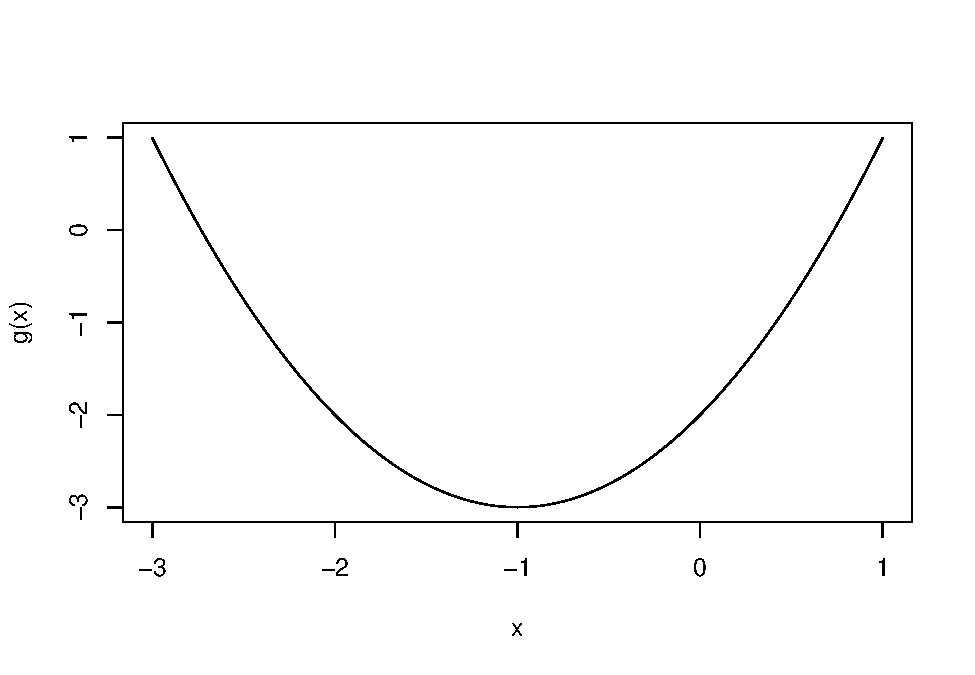
\includegraphics{R-ohjelmoinnin-perusteet_files/figure-latex/unnamed-chunk-184-1.pdf}

Kuvan perusteella minimiarvo saavutetaan pisteessä \(x = -1\). Käytetään nyt \texttt{optimize} funktiota:

\begin{Shaded}
\begin{Highlighting}[]
\FunctionTok{optimize}\NormalTok{(g, }\AttributeTok{interval =} \FunctionTok{c}\NormalTok{(}\SpecialCharTok{{-}}\DecValTok{3}\NormalTok{, }\DecValTok{1}\NormalTok{))}
\end{Highlighting}
\end{Shaded}

\begin{verbatim}
## $minimum
## [1] -1
## 
## $objective
## [1] -3
\end{verbatim}

Funktion palauttmassa listassa alkio \texttt{minimum} ilmoittaa pisteen, jossa minimi saavutetaan. Alkio \texttt{objective} antaa tavoitefunktion (eli funktion \texttt{f}) arvon kyseisessä psiteessä.

\hypertarget{useampi-parametri}{%
\subsection{Useampi parametri}\label{useampi-parametri}}

Mikäli funktiota halutaan minimoida useamman kuin yhden parametrin suhteen, voidaan käyttää funktiota \texttt{optim}.

\begin{Shaded}
\begin{Highlighting}[]
\FunctionTok{optim}\NormalTok{(par, fn, }\AttributeTok{gr =} \ConstantTok{NULL}\NormalTok{, ...,}
      \AttributeTok{method =} \FunctionTok{c}\NormalTok{(}\StringTok{"Nelder{-}Mead"}\NormalTok{, }\StringTok{"BFGS"}\NormalTok{, }\StringTok{"CG"}\NormalTok{, }\StringTok{"L{-}BFGS{-}B"}\NormalTok{, }\StringTok{"SANN"}\NormalTok{,}
                 \StringTok{"Brent"}\NormalTok{),}
      \AttributeTok{lower =} \SpecialCharTok{{-}}\ConstantTok{Inf}\NormalTok{, }\AttributeTok{upper =} \ConstantTok{Inf}\NormalTok{,}
      \AttributeTok{control =} \FunctionTok{list}\NormalTok{(), }\AttributeTok{hessian =} \ConstantTok{FALSE}\NormalTok{)}
\end{Highlighting}
\end{Shaded}

Ensimmäinen argumentti \texttt{par} on vektori, joka antaa alkuarvot jokaiselle parametrille, jonka suhteen minimointia halutaan tehdä. Seuraava argumentti \texttt{fn} on minimoivata funktio, jonka ensimmäisen argumentin tulee vastata argumenttia \texttt{par} (vektori, jossa on yhtä monta alkiota). Vastaavasti kuten \texttt{optimize}-funktiossa, argumentit \texttt{lower} ja \texttt{upper} määrittävä alueen, jolta minimiä etsitään. Huomaa kuitenkin, että koska funktiolla \texttt{fn} on nyt useampi parametri, ovat \texttt{lower} ja \texttt{upper} myös vektoreita jotka ilmoittavat rajat jokaiselle parametrille erikseen. Alkuarvojen \texttt{par} on myös toteutettava mahdolliset rajoitteet. Argumentti \texttt{method} valitsee käytettävän optimointimenetelmän. Metelmistä riittää tietää tässä vaiheessa se, että jos optimointia halutaan tehdä käyttäen rajoitteita (\texttt{lower} ja \texttt{upper}), voidaan menetelmäksi valita ``L-BFGS-B'', muuten voidaan käyttää oletusarvoa. Muista \texttt{optim}-funktion argumenteista ei tämän kurssin puitteissa tarvitse välittää.

Etsitään funktion \(f(x,y) = y^2\exp(-0.5(y^2+x^2))\) lokaali maksimi joukossa \(-1 < x < 3\), \$ -1 \textless{} y \textless{} 3\$. Annetaan alkuarvoiksi \(x = 0.5\) ja \(y = 0.5\). \texttt{optim}-funktio etsii oletusarvoisesti funktion minimiä, joten vaihtamalla funktion merkki etsitäänkin maksimia. Huomaa, että funktiolla \texttt{f} on vain yksi argumentti \texttt{x}, vaikka funktiolla \(f\) on kaksi argumenttia, \(x\) ja \(y\). Tämä johtuu siitä, että \texttt{optim}-funktion tapauksessa parametrien \texttt{par} on esiinnyttävä funktion argumenteissa vektorina. Vektorin \texttt{x} ensimmäinen alkio \texttt{x{[}1{]}} vastaa siis muuttujaa \(x\) ja toinen alkio \texttt{x{[}2{]}} vastaa muuttujaa \(y\). Tämä yleistyy useamman kuin kahden muuttujan funktioille, kun vektorin \texttt{x} pituutta kasvatetaan vastaavasti (esim. kolmas muuttuja \(z\) olisi \texttt{x{[}3{]}} jne.).

\begin{Shaded}
\begin{Highlighting}[]
\NormalTok{f }\OtherTok{\textless{}{-}} \ControlFlowTok{function}\NormalTok{(x) }\SpecialCharTok{{-}}\NormalTok{x[}\DecValTok{2}\NormalTok{]}\SpecialCharTok{\^{}}\DecValTok{2} \SpecialCharTok{*} \FunctionTok{exp}\NormalTok{(}\SpecialCharTok{{-}}\FloatTok{0.5} \SpecialCharTok{*}\NormalTok{ (x[}\DecValTok{2}\NormalTok{]}\SpecialCharTok{\^{}}\DecValTok{2} \SpecialCharTok{+}\NormalTok{ x[}\DecValTok{1}\NormalTok{]}\SpecialCharTok{\^{}}\DecValTok{2}\NormalTok{))}
\FunctionTok{optim}\NormalTok{(}\FunctionTok{c}\NormalTok{(}\FloatTok{0.5}\NormalTok{, }\FloatTok{0.5}\NormalTok{), f, }\AttributeTok{lower =} \FunctionTok{c}\NormalTok{(}\SpecialCharTok{{-}}\DecValTok{1}\NormalTok{, }\SpecialCharTok{{-}}\DecValTok{1}\NormalTok{), }\AttributeTok{upper =} \FunctionTok{c}\NormalTok{(}\DecValTok{3}\NormalTok{, }\DecValTok{3}\NormalTok{), }\AttributeTok{method =} \StringTok{"L{-}BFGS{-}B"}\NormalTok{)}
\end{Highlighting}
\end{Shaded}

\begin{verbatim}
## $par
## [1] -7.582426e-10  1.414214e+00
## 
## $value
## [1] -0.7357589
## 
## $counts
## function gradient 
##        8        8 
## 
## $convergence
## [1] 0
## 
## $message
## [1] "CONVERGENCE: REL_REDUCTION_OF_F <= FACTR*EPSMCH"
\end{verbatim}

Funktion palauttamassa tulosteessa \texttt{par} kertoo maksimipisteen koordinaatit. Ensimmäinen alkio kertoo maksimipisteen \(x\)-koordinaatin, ja toinen sen \(y\)-koordinaatin (huomioi erityisesti 1. alkion merkintätapa \texttt{-7.582426e-10} joka tarkoittaa samaa kuin \(-7.582426 \cdot 10^{-10}\), eli noin \(0.00000000076\), eli \(x\) koordinaatti on siis käytännössä \(0\)). \texttt{value} ilmoittaa löydettyä maksimipistettä vastaavan funktion arvon. Koska funktion merkki vaihdettiin maksimin etsimiseksi, on todellinen maksimiarvo siis löydetyn optimin vastaluku, eli \(\approx 0.7357589\). Muut tulostukset ovat optimoinnin konvergenssiin liittyviä lisätietoja. Vaihtoehtoisesti maksimia voi etsiä suoraankin vaihtamatta funktion merkkiä antamalla \texttt{optim}-funktiolle lisäargumentti \texttt{control\ =\ list(fnscale\ =\ -1)}.

Etsitään vielä kolmen muuttujan funktion \(h(x,y,z) = \exp(-x^2-3x-7y^2+3y+z^3-2z-3)\) lokaali maksimi joukossa \(-2 < x < 2\), \$ -3 \textless{} y \textless{} 3\$, \(-3 < z < 0\).

\begin{Shaded}
\begin{Highlighting}[]
\NormalTok{h }\OtherTok{\textless{}{-}} \ControlFlowTok{function}\NormalTok{(x) }\FunctionTok{exp}\NormalTok{(}\SpecialCharTok{{-}}\NormalTok{x[}\DecValTok{1}\NormalTok{]}\SpecialCharTok{\^{}}\DecValTok{2} \SpecialCharTok{{-}} \DecValTok{3}\SpecialCharTok{*}\NormalTok{x[}\DecValTok{1}\NormalTok{] }\SpecialCharTok{{-}} \DecValTok{7}\SpecialCharTok{*}\NormalTok{x[}\DecValTok{2}\NormalTok{]}\SpecialCharTok{\^{}}\DecValTok{2} \SpecialCharTok{+} \DecValTok{3}\SpecialCharTok{*}\NormalTok{x[}\DecValTok{2}\NormalTok{] }\SpecialCharTok{+}\NormalTok{ x[}\DecValTok{3}\NormalTok{]}\SpecialCharTok{\^{}}\DecValTok{3} \SpecialCharTok{{-}} \DecValTok{2}\SpecialCharTok{*}\NormalTok{x[}\DecValTok{3}\NormalTok{] }\SpecialCharTok{{-}} \DecValTok{3}\NormalTok{)}
\FunctionTok{optim}\NormalTok{(}\FunctionTok{c}\NormalTok{(}\FloatTok{0.5}\NormalTok{, }\FloatTok{0.5}\NormalTok{, }\SpecialCharTok{{-}}\FloatTok{0.5}\NormalTok{), h, }\AttributeTok{lower =} \FunctionTok{c}\NormalTok{(}\SpecialCharTok{{-}}\DecValTok{2}\NormalTok{, }\SpecialCharTok{{-}}\DecValTok{3}\NormalTok{, }\SpecialCharTok{{-}}\DecValTok{3}\NormalTok{), }\AttributeTok{upper =} \FunctionTok{c}\NormalTok{(}\DecValTok{2}\NormalTok{, }\DecValTok{3}\NormalTok{, }\DecValTok{0}\NormalTok{), }
      \AttributeTok{method =} \StringTok{"L{-}BFGS{-}B"}\NormalTok{, }\AttributeTok{control =} \FunctionTok{list}\NormalTok{(}\AttributeTok{fnscale =} \SpecialCharTok{{-}}\DecValTok{1}\NormalTok{))}
\end{Highlighting}
\end{Shaded}

\begin{verbatim}
## $par
## [1] -1.5000009  0.2142866 -0.8164968
## 
## $value
## [1] 1.934968
## 
## $counts
## function gradient 
##       22       22 
## 
## $convergence
## [1] 0
## 
## $message
## [1] "CONVERGENCE: REL_REDUCTION_OF_F <= FACTR*EPSMCH"
\end{verbatim}

Kuten edellä, \texttt{par} ilmoittaa maksimipisteen koordinaatit. Maksimi saavutetaan siis pisteessä \((x,y,z) \approx (-1.5000009, 0.2142866, -0.8164968)\) jolloin funktio \(h\) saa kohdan \texttt{value} ilmoittaman arvon \(\approx 1.934968\). Nyt koska käytettiin argumenttia \texttt{control\ =\ list(fnscale\ =\ -1)}, ei tuloksen merkkiä tarvitse vaihtaa.

Alkuarvot funktioille \texttt{optim} ja \texttt{optimize} tulee valita siten, että rajoitteet ovat voimassa. Alkuarvojen valintaan on vaikea antaa yleispätevää ohjetta, ja usein onkin hyvä kokeilla eri arvoja ja verrata niillä saatuja tuloksia. Yhden ja kahden muuttujan tapauksissa löydettyjen optimipisteiden mielekkyyttä voi tarkastella esimerkiksi piirtämällä funktion kuvaajan annetussa joukossa.

\hypertarget{funktion-juurten-etsintuxe4}{%
\section{Funktion juurten etsintä}\label{funktion-juurten-etsintuxe4}}

Funktion juuria voidaan etsiä funktiolla \texttt{uniroot}.

\begin{Shaded}
\begin{Highlighting}[]
\FunctionTok{uniroot}\NormalTok{(f, interval, ...,}
        \AttributeTok{lower =} \FunctionTok{min}\NormalTok{(interval), }\AttributeTok{upper =} \FunctionTok{max}\NormalTok{(interval),}
        \AttributeTok{f.lower =} \FunctionTok{f}\NormalTok{(lower, ...), }\AttributeTok{f.upper =} \FunctionTok{f}\NormalTok{(upper, ...),}
        \AttributeTok{extendInt =} \FunctionTok{c}\NormalTok{(}\StringTok{"no"}\NormalTok{, }\StringTok{"yes"}\NormalTok{, }\StringTok{"downX"}\NormalTok{, }\StringTok{"upX"}\NormalTok{), }\AttributeTok{check.conv =} \ConstantTok{FALSE}\NormalTok{,}
        \AttributeTok{tol =}\NormalTok{ .Machine}\SpecialCharTok{$}\NormalTok{double.eps}\SpecialCharTok{\^{}}\FloatTok{0.25}\NormalTok{, }\AttributeTok{maxiter =} \DecValTok{1000}\NormalTok{, }\AttributeTok{trace =} \DecValTok{0}\NormalTok{)}
\end{Highlighting}
\end{Shaded}

Funktion \texttt{f} juuria etsitään annetulta väliltä \texttt{interval}, sen ensimmäisen argumentin suhteen (jonka tulee olla skalaari). Halutun välin voi määrittää myös sen päätepisteinä käyttäen argumentteja \texttt{lower} ja \texttt{upper}. Muut \texttt{uniroot}-funktion argumentit eivät ole tämän kurssin kannalta oleellisia.

Etsitään funktion \(w(x)=x^3-2x-5\) juurta väliltä \((-5,5)\).

\begin{Shaded}
\begin{Highlighting}[]
\NormalTok{w }\OtherTok{\textless{}{-}} \ControlFlowTok{function}\NormalTok{(x) \{ x}\SpecialCharTok{\^{}}\DecValTok{3} \SpecialCharTok{{-}} \DecValTok{2}\SpecialCharTok{*}\NormalTok{x }\SpecialCharTok{{-}} \DecValTok{5}\NormalTok{ \}}
\FunctionTok{uniroot}\NormalTok{(w, }\AttributeTok{interval =} \FunctionTok{c}\NormalTok{(}\SpecialCharTok{{-}}\DecValTok{5}\NormalTok{, }\DecValTok{5}\NormalTok{))}
\end{Highlighting}
\end{Shaded}

\begin{verbatim}
## $root
## [1] 2.094528
## 
## $f.root
## [1] -0.0002653143
## 
## $iter
## [1] 9
## 
## $init.it
## [1] NA
## 
## $estim.prec
## [1] 6.103516e-05
\end{verbatim}

Funktion palauttamassa tulosteessa kohta \texttt{root} ilmoittaa löydetyn juuren. Mikäli juurta ei löydy annetulta väliltä, funktio antaa varoituksen. Kohta \texttt{froot} ilmoittaa funktion arvon löydetyssä pisteessä (funktion arvon ja nollan ero riippuu laskennan tarkkuudesta ja käytetystä menetelmästä).

\hypertarget{numeerinen-integrointi}{%
\section{Numeerinen integrointi}\label{numeerinen-integrointi}}

R:n optimointityökaluihin kuuluu myös funktio \texttt{integrate}, jolla voi laskea useimpien funktioiden määrättyjä integraaleja.

\begin{Shaded}
\begin{Highlighting}[]
\FunctionTok{integrate}\NormalTok{(f, lower, upper, ..., }\AttributeTok{subdivisions =}\NormalTok{ 100L,}
          \AttributeTok{rel.tol =}\NormalTok{ .Machine}\SpecialCharTok{$}\NormalTok{double.eps}\SpecialCharTok{\^{}}\FloatTok{0.25}\NormalTok{, }\AttributeTok{abs.tol =}\NormalTok{ rel.tol,}
          \AttributeTok{stop.on.error =} \ConstantTok{TRUE}\NormalTok{, }\AttributeTok{keep.xy =} \ConstantTok{FALSE}\NormalTok{, }\AttributeTok{aux =} \ConstantTok{NULL}\NormalTok{)}
\end{Highlighting}
\end{Shaded}

Ensimmäinen argumentti \texttt{f} on funktio, jota halutaan integroida. Argumentit \texttt{lower} ja \texttt{upper} määräävät integrointivälin, jonka päätepisteet voivat olla myös äärettömiä. Tällöin voidaan asettaa \texttt{lower\ =\ -Inf} tai vastaavasti \texttt{upper\ =\ Inf}..

Integroidaan funktiota \(f(x) = x^2+3x-2\) välin \([-2,3]\) yli.

\begin{Shaded}
\begin{Highlighting}[]
\NormalTok{poly }\OtherTok{\textless{}{-}} \ControlFlowTok{function}\NormalTok{(x) \{ x}\SpecialCharTok{\^{}}\DecValTok{2} \SpecialCharTok{+} \DecValTok{3}\SpecialCharTok{*}\NormalTok{x }\SpecialCharTok{{-}} \DecValTok{2}\NormalTok{ \}}
\FunctionTok{integrate}\NormalTok{(poly, }\SpecialCharTok{{-}}\DecValTok{2}\NormalTok{, }\DecValTok{3}\NormalTok{)}
\end{Highlighting}
\end{Shaded}

\begin{verbatim}
## 9.166667 with absolute error < 2.8e-13
\end{verbatim}

Integraalin arvo on siis noin \(9.17\).

\end{document}
